%%!TEX encoding = UTF-8 Unicode

% Several lines in file have comments suggesting common packages for the
% typical thesis in informatics or electronics developed at UA
% uncomment/comment the lines as required for your work
% Before each optional line you will have a small comment

% According to UA rules, font size should range from 10 to 12pt.
\documentclass[10pt,a4paper,openright,twoside,onecolumn]{memoir}

\listfiles
\fixpdflayout

\usepackage[utf8]{inputenc}

% Select Computer Modern Typewritter (For bold ttfamily in listings)
\usepackage{lmodern}
% OR... Bera Mono
%\usepackage[scaled]{beramono} % TTT Font
%\usepackage{anyfontsize} % As the name says...

\usepackage[T1]{fontenc}

% Enable for for Overleaf support
\usepackage{ifthen}
\def\useoverleaf{0}  % change to non-zero (for instance, 1) to enable it

\makeatletter
\newcommand{\makecoverfile}[0]{%
  \immediate\write18{latexmk -pdf cover.tex}%
}
\makeatother

% For PDF merging
\usepackage{pdfpages}

% Set DPI to 300
\pdfpxdimen=\dimexpr 1in/300\relax

% Allow the use of a larger number of packages
\usepackage{morewrites} 

% For English and Portuguese languages
% Portuguese will be the default.
% Uncomment \setlanguage below to change it
\usepackage[english,portuguese]{babel}

% Uncomment to use a custom date format
%\usepackage{datetime}
%\newdateformat{thesisdate}{\monthname[\THEMONTH] \THEYEAR} % Month Year

% Make pdf look better
\usepackage{microtype} 

% Uncomment to enable floats on facing pages
%\usepackage{dpfloat}

% Side by side figures
% Eg. Fig 1a, Fig 1b
\usepackage[hang,small,bf]{caption}
%\let\tion\undefined
%\let\subfloat\undefined
\usepackage{subcaption}

%\RequirePackage{textcase}

% Dropped Caps
%\usepackage{lettrine}

% Configure Hyperlink color
% As a matter or style, you may use this to enable/disable color boxes on links
%\usepackage[breaklinks=true,colorlinks=false,linkcolor=blue]{hyperref}
% Or use the default values provided by the hyperref package
\usepackage{hyperref}

% Redefine section names according to your preference
%\def\sectionautorefname{Section}
%\def\chapterautorefname{Chapter}
%\def\figureautorefname{Figure}
%\def\listingautorefname{Listing}
%\def\tableautorefname{Table}

% Redefine code boxes
\ifthenelse{\equal{\useoverleaf}{0}}
{\usepackage[cache=false]{minted}}
{\usepackage[cache=false]{minted}}%

\addto\captionsportuguese{%
  \renewcommand\listingscaption{Code Snippet}
}
\fvset{fontsize=\footnotesize} % Make Code blocks smaller than text
\usepackage{csquotes}

% Add support for PDF Comments
\usepackage{comment}
\ifthenelse{\equal{\useoverleaf}{0}}
{\usepackage{pdfcomment}}{}
\usepackage{bookmark} % New Bookmarks

% For Multiple columns in Glossary
\usepackage{multicol}
% For Multiple rows
\usepackage{multirow}

% Add support for Math symbols
\usepackage{amsmath}
\usepackage{amssymb}

% Add support for graphics
\usepackage{graphicx}

% Add support for Colors
\usepackage{xcolor,colortbl}

% Add support for the Euro symbol
\usepackage{eurosym}

% Enumerate in line
\usepackage[inline]{enumitem}

% Setup bibliography with Biber using IEEE style for proper UTF-8 support
\usepackage[backend=biber,style=ieee, sorting=none]{biblatex}
\bibliography{bib/references.bib, bib/rfc.bib}

% Use acronyms
\usepackage[printonlyused]{acronym} % For acronyms

% Indenting the first paragraph after section start
\usepackage{indentfirst}

% Uncomment the next lines to enable chart support through pgf and tikz
% This may require you to install further packages in your Tex system
%\usepackage[version=0.96]{pgf}
%\usepackage{tikz}

% UML support
%\usepackage{pgf-umlsd}

% Trees, Arrows, Mindmaps and other popular objects
%\usetikzlibrary{arrows,shadows,trees,shapes,decorations,automata,backgrounds,petri,mindmap} % for pgf-umlsd

% Package to master SI units
\usepackage[detect-weight=true, binary-units=true]{siunitx}
% For Electric Circuits
%\sisetup{load-configurations = binary}

% Set Voltage direction accordingly
% Option : oldvoltagedirection,nooldvoltagedirection,RPvoltages,EFvoltages
% More information at: https://mirrors.ibiblio.org/CTAN/graphics/pgf/contrib/circuitikz/doc/circuitikzmanual.pdf
% By default this template is using the Old Voltage Direction
%\usepackage[oldvoltagedirection,american,cuteinductors,smartlabels]{circuitikz}
%\usetikzlibrary{calc}
%\ctikzset{bipoles/thickness=1}
%\ctikzset{bipoles/length=0.8cm}
%\ctikzset{bipoles/diode/height=.375}
%\ctikzset{bipoles/diode/width=.3}
%\ctikzset{tripoles/thyristor/height=.8}
%\ctikzset{tripoles/thyristor/width=1}
%\ctikzset{bipoles/vsourceam/height/.initial=.7}
%\ctikzset{bipoles/vsourceam/width/.initial=.7}
%\tikzstyle{every node}=[font=\small]
%\tikzstyle{every path}=[line width=0.8pt,line cap=round,line join=round]

% For inline TT text (e.g. code snippets)
\usepackage{verbatim}

% Frames around figures and allow force placement
\usepackage{float}

% Configure Float style
%\floatstyle{boxed}
%\restylefloat{table}
%\restylefloat{figure}
%\restylefloat{lstlisting}

% For test purposes you may use the lipsum package to create dummy text
\usepackage{lipsum} % REMOVE

%Keep floats inside section!
\usepackage[section]{placeins}
\let \oldsubsubsection \subsubsection
\renewcommand{\subsubsection}[2][]{
  \FloatBarrier
  \oldsubsubsection#1{#2}
}
\let \oldsubsection \subsection
\renewcommand{\subsection}[2][]{
  \FloatBarrier
  \oldsubsection#1{#2}
}
\let \oldsection \section
\renewcommand{\section}[2][]{
  \FloatBarrier
  \oldsection#1{#2}
}
\let \oldchapter \chapter
\renewcommand{\chapter}[2][]{
  \FloatBarrier
  \oldchapter#1{#2}
}


% Use the built-in division styling
\headstyles{memman}

% Include subsections in the TOC
\settocdepth{subsection}

% Numbering down to subsections as well
\setsecnumdepth{subsection}

% extra index for first lines
\makeindex[lines]

% Margins for University of Aveiro Thesis
\setlrmarginsandblock{3cm}{2.5cm}{*}
\setulmarginsandblock{3cm}{3cm}{*}
\checkandfixthelayout

% Or select your custom spacing to make any ajustment
%\addtolength{\parskip}{0.5\baselineskip}
\linespread{1.5}


%%%%%%%%%%%%%%%%%%%%%%%%%%%%%%%%%%%%%%%%%%%%%%%%%%
% Document begins here
%%%%%%%%%%%%%%%%%%%%%%%%%%%%%%%%%%%%%%%%%%%%%%%%%%

\begin{document}
\ifthenelse{\equal{\useoverleaf}{0}}{}{\makecoverfile{}}%
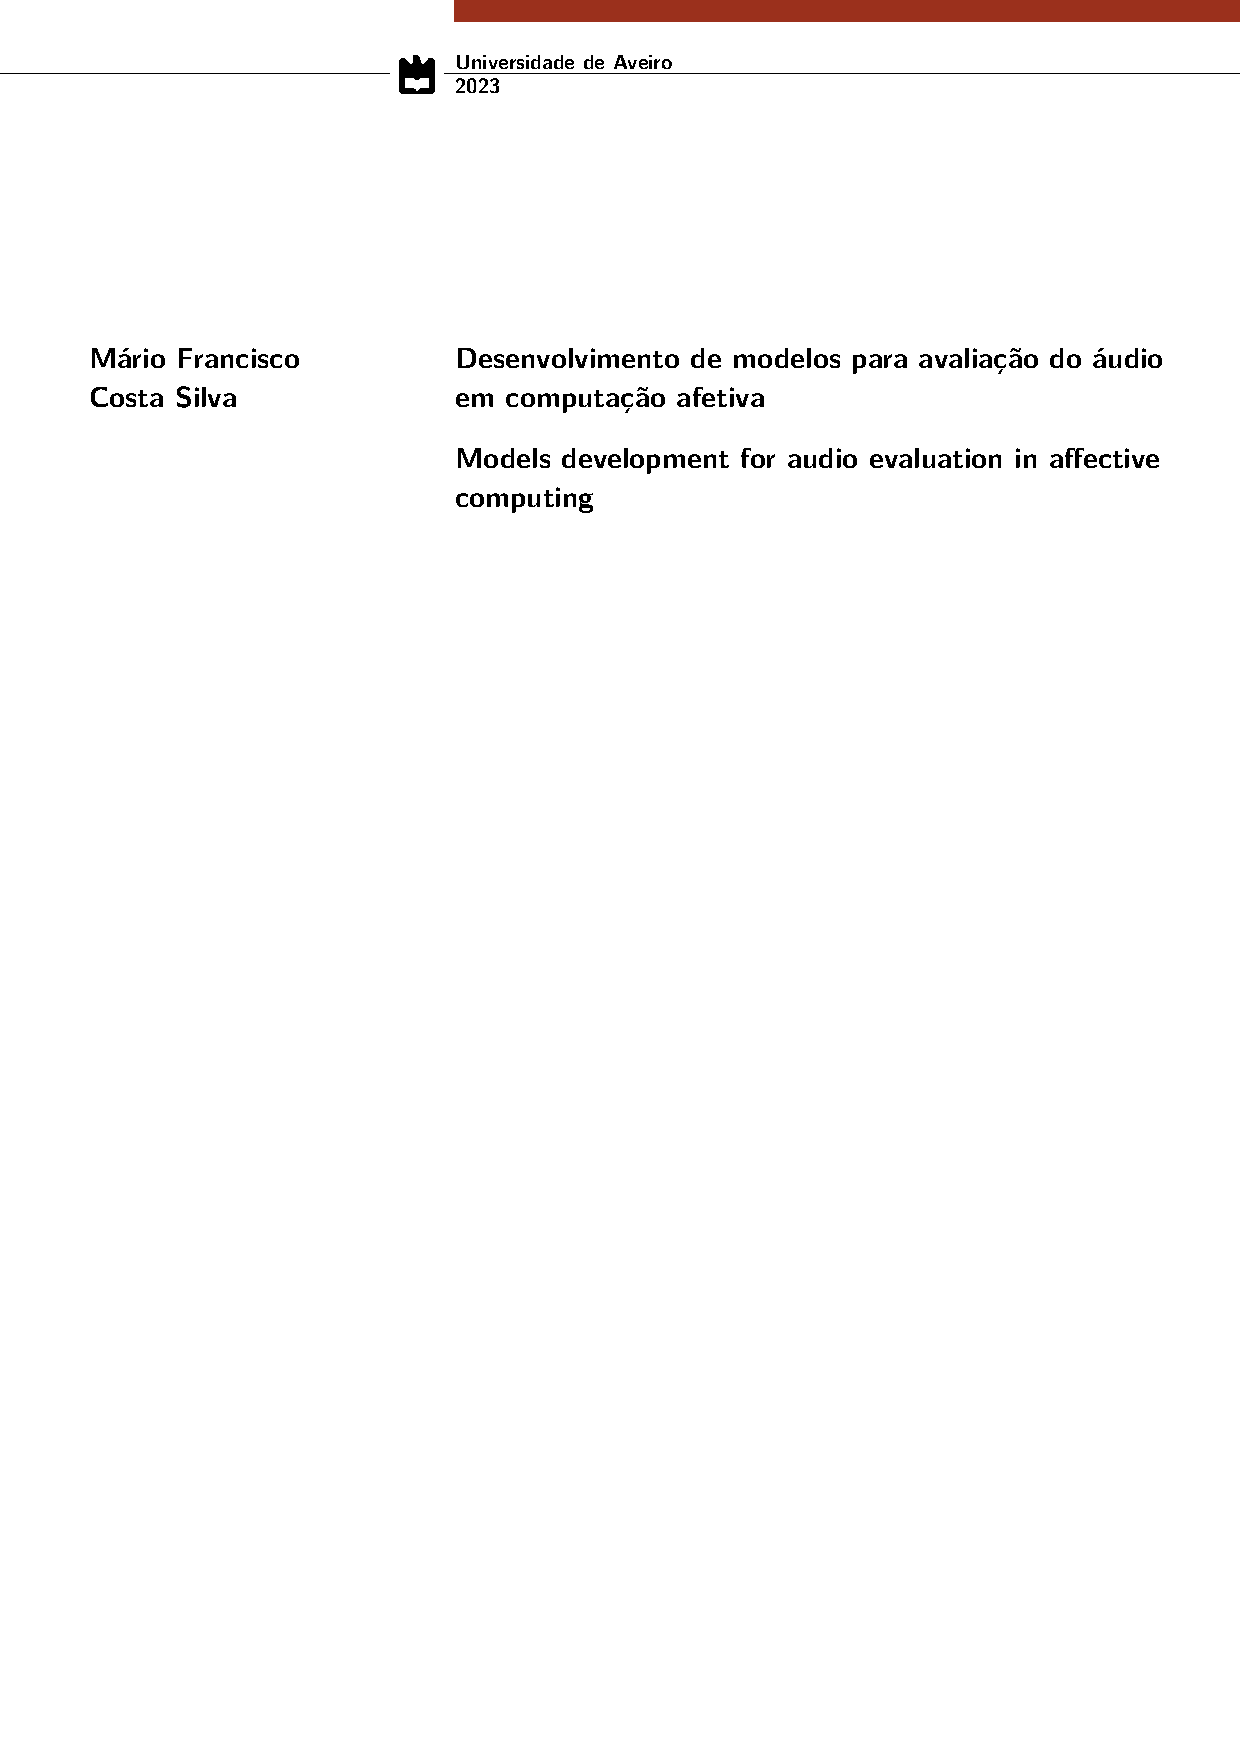
\includepdf[pages=-]{cover.pdf}

% Uncomment to enable English
\selectlanguage{english}

% Front matter

%Custom Chapter style named `thesis`
\makechapterstyle{thesis}{% Based on ell
  \chapterstyle{default}
  \renewcommand*{\chapnumfont}{\normalfont\sffamily}
  \renewcommand*{\chaptitlefont}{\normalfont\Huge\sffamily}
  \settowidth{\chapindent}{\chapnumfont 111}
  \renewcommand*{\chapterheadstart}{\begingroup
    \vspace*{\beforechapskip}%
    \begin{adjustwidth}{}{-\chapindent}%
    \hrulefill
    \smash{\rule{0.4pt}{15mm}}
    \end{adjustwidth}\endgroup}
  \renewcommand*{\printchaptername}{}
  \renewcommand*{\chapternamenum}{}
  \renewcommand*{\printchapternum}{%
    \begin{adjustwidth}{}{-\chapindent}
    \hfill
    \raisebox{10mm}[0pt][0pt]{\fontsize{30}{25}\selectfont\chapnumfont \thechapter}%
                              \hspace*{1em}
    \end{adjustwidth}\vspace*{-3.0\onelineskip}}
  \renewcommand*{\printchaptertitle}[1]{%
    \vskip\onelineskip
    \raggedleft {\chaptitlefont ##1}\par\nobreak\vskip 4\onelineskip}}


% Select chapter style from existing or select custom
%\chapterstyle{thesis} % Others: dowding, demo2, dash, chappell, brotherton, bianchi, ger, madsen, tatcher, veelo,indexes)
% thesis can also be used as defined previously
% Check the memoir documentation for the available themes
% Default is veelo
\chapterstyle{veelo}
\makeoddfoot{plain}{}{\thepage}{} % Added by André Zúquete to fix a page numbering issue on the veelo chapter style


% If you feel adventurous you can also define all aspects of your theme
% Use either this input or the chapterstyle before
% % Rules
\newcommand{\thinRule}{\rule{\textwidth}{0.25pt}}

% Customize heading appearances
% Define styles
\newcommand{\partSize}{\Huge}
\newcommand{\partStyle}{\lsstyle\scshape}
\newcommand{\chapterSize}{\Huge}
\newcommand{\chapterStyle}{\lsstyle\scshape}
\newcommand{\chapterAfter}{}
\newcommand{\sectionSize}{\Large}
\newcommand{\sectionStyle}{\scshape\MakeTextLowercase}
\newcommand{\subsectionSize}{\large}
\newcommand{\subsectionStyle}{\scshape\MakeTextLowercase}
\newcommand{\subsubsectionSize}{\large}
\newcommand{\subsubsectionStyle}{\scshape\MakeTextLowercase}
\newlength{\partNumSizePt}
\setlength{\partNumSizePt}{60pt}
\newlength{\chapterNumSizePt}
\setlength{\chapterNumSizePt}{60pt}
\newcommand{\partNumSize}{%
  \fontsize{\partNumSizePt}{1.2\partNumSizePt}\selectfont%
}
\newcommand{\partNumStyle}{\partChapterNumColor}
\newcommand{\chapterNumSize}{%
  \fontsize{\chapterNumSizePt}{1.2\chapterNumSizePt}\selectfont%
}
\newcommand{\chapterNumStyle}{\partChapterNumColor}

% Customize parts
\renewcommand{\partnamefont}{\partSize\partStyle}
\renewcommand{\partnumfont}{\partNumSize\partNumStyle}
\renewcommand{\printpartname}{}
\renewcommand{\printparttitle}[1]{%
  \normalfont\normalcolor\partnamefont #1
}

% Customize chapters
\makeatletter
\setlength{\beforechapskip}{30pt}
\renewcommand*{\chapterheadstart}{\vspace*{\beforechapskip}}
\setlength{\afterchapskip}{3ex}
\setlength{\midchapskip}{3ex}
\renewcommand*{\chapnamefont}{%
  \Large\flushright\chapterStyle\partChapterNumColor%
}
\renewcommand*{\chapnumfont}{\chapterNumSize\chapterNumStyle}
\renewcommand*{\chaptitlefont}{%
  \normalfont\flushleft\normalcolor\chapterSize\chapterStyle%
}
\renewcommand*{\printchaptername}{%
  \chapnamefont\MakeTextLowercase{\@chapapp}%
}
\renewcommand*{\chapternamenum}{\quad}
\renewcommand*{\printchapternum}{%
%  \chapnumfont\textls[-75]{\classicstylenums{\thechapter}}%
 \chapnumfont\textls[-75]{\thechapter}%

}
\renewcommand*{\printchaptertitle}[1]{%
  \chaptitlefont #1
  \chapterAfter
}
\makeatother
% Customize sections and subsections
\setsecnumformat{\csname my#1\endcsname\quad}
\setsecheadstyle{\sectionSize\sectionStyle}
\newcommand{\mysection}{{\thesection}}
\setlength{\beforesecskip}{3em}


\setsubsecheadstyle{\subsectionSize\subsectionStyle}
\newcommand{\mysubsection}{{\normalfont\subsectionSize\thesubsection}}
\setlength{\beforesubsecskip}{3em}

\setsubsubsecheadstyle{\subsubsectionSize\subsubsectionStyle}
\newcommand{\mysubsubsection}{{\normalfont\subsubsectionSize\thesubsubsection}}
\setlength{\beforesubsubsecskip}{2em}

% Customize "Table of ..." appearance
% Customize headings
\newcommand{\renewPrintXTitle}[1]{%
  \renewcommand{#1}[1]{%
    \printchaptertitle{##1}%
  }%
}
\renewPrintXTitle{\printtoctitle}
\renewPrintXTitle{\printlottitle}
\renewPrintXTitle{\printloftitle}

% Customize ToC headings
\renewcommand{\cftpartfont}{\partChapterNumColor\partStyle}
\renewcommand{\cftchapterfont}{\chapterStyle}
\renewcommand{\cftsectionfont}{}
\renewcommand{\cftsubsectionfont}{}
\renewcommand{\cftfigurefont}{}
\renewcommand{\cfttablefont}{}
\newcommand{\cftlstlistingfont}{}

% Increase number width
\newlength{\cftNumWidthIncrease}
\setlength{\cftNumWidthIncrease}{0.25em}
\addtolength{\cftpartnumwidth}{\cftNumWidthIncrease}
\addtolength{\cftchapternumwidth}{\cftNumWidthIncrease}
\addtolength{\cftsectionindent}{\cftNumWidthIncrease}
\addtolength{\cftsubsectionindent}{\cftNumWidthIncrease}
% No leader dots
%\renewcommand*{\cftpartdotsep}{\cftnodots}
%\renewcommand*{\cftchapterdotsep}{\cftnodots}
%\renewcommand*{\cftsectiondotsep}{\cftnodots}
%\renewcommand*{\cftsubsectiondotsep}{\cftnodots}
%\renewcommand*{\cftfiguredotsep}{\cftnodots}
%\renewcommand*{\cfttabledotsep}{\cftnodots}
%\newcommand*{\cftlstlistingdotsep}{\cftnodots}
% Set page numbers immediately after entry text
\newcommand{\tocEntryPageSep}{\hspace{1em}}
\renewcommand{\cftpartleader}{\cftdotfill{\cftdotsep}}
%\renewcommand{\cftpartafterpnum}{\cftparfillskip}
%\renewcommand{\cftchapterleader}{\tocEntryPageSep}
\renewcommand{\cftchapterleader}{\cftdotfill{\cftdotsep}}
%\renewcommand{\cftchapterafterpnum}{\cftparfillskip}
\renewcommand{\cftsectionleader}{\cftdotfill{\cftdotsep}}
%\renewcommand{\cftsectionafterpnum}{\cftparfillskip}
\renewcommand{\cftsubsectionleader}{\cftdotfill{\cftdotsep}}
%\renewcommand{\cftsubsectionafterpnum}{\cftparfillskip}
\renewcommand{\cftfigureleader}{\cftdotfill{\cftdotsep}}
%\renewcommand{\cftfigureafterpnum}{\cftparfillskip}
\renewcommand{\cfttableleader}{\cftdotfill{\cftdotsep}}
%\renewcommand{\cfttableafterpnum}{\cftparfillskip}
\newcommand{\cftlstlistingleader}{\cftdotfill{\cftdotsep}}
%\newcommand{\cftlstlistingafterpnum}{\cftparfillskip}
% Customize page numbers
\newcommand{\tocPageStyle}{\tocPageColor}
\renewcommand{\cftpartpagefont}{\tocPageStyle}
\renewcommand{\cftchapterpagefont}{\tocPageStyle}
\renewcommand{\cftsectionpagefont}{\tocPageStyle}
\renewcommand{\cftsubsectionpagefont}{\tocPageStyle}
\renewcommand{\cftfigurepagefont}{\tocPageStyle}
\renewcommand{\cfttablepagefont}{\tocPageStyle}
\newcommand{\cftlstlistingpagefont}{\tocPageStyle}

% Abstract
% Remove indents around abstract text
\setlength{\absleftindent}{0pt}
\setlength{\absrightindent}{0pt}
% Change font size to conform with the rest of the document text
\renewcommand{\abstracttextfont}{\normalsize}

% Customize headers and footers including page numbers
\newcommand{\hfTextSize}{\footnotesize}
\newcommand{\headTextStyle}{\lsstyle\scshape\MakeTextLowercase}
\nouppercaseheads
\makeevenhead{headings}%
             {\hfTextSize\thepage}%
             {}%
             {\hfTextSize\headTextStyle\leftmark}
\makeevenhead{plain}%
             {\hfTextSize\thepage}%
             {}%
             {\hfTextSize\headTextStyle\leftmark}
\makeoddhead{headings}%
            {\hfTextSize\headTextStyle\rightmark}%
            {}%
            {\hfTextSize\thepage}
\makeoddhead{plain}%
            {\hfTextSize\headTextStyle\rightmark}%
            {}%
            {\hfTextSize\thepage}


% Customize captions
\newcommand{\captionSize}{\small}
\newcommand{\captionStyle}{\scshape}
\newcommand{\captionWidthRatio}{0.9}

\captionnamefont{\captionSize\captionStyle}
\captiontitlefont{\captionSize}
\captiondelim{ -- }
\captiontitlefinal{}
\changecaptionwidth
%\captionwidth{\captionWidthRatio\textwidth}

% Define colors
%\newcommand{\titleColor}{\color[rgb]{0.616, 0.0627, 0.176}}
\newcommand{\titleColor}{\color[rgb]{0,0,0}}

\newcommand{\partChapterNumColor}{\titleColor}
\newcommand{\dropCapColor}{\titleColor}
%\newcommand{\tocPageColor}{\color[rgb]{0.0980, 0.329, 0.651}}

\newcommand{\tocPageColor}{\color[rgb]{0, 0,0}}
\definecolor{shade0}{rgb}{1.0 , 1.0 , 1.0 }
\definecolor{shade1}{rgb}{0.9 , 0.9 , 0.9 }
\definecolor{shade2}{rgb}{0.8 , 0.8 , 0.8 }
\definecolor{shade3}{rgb}{0.65, 0.65, 0.65}
\definecolor{shade4}{rgb}{0.45, 0.45, 0.45}
\definecolor{shade5}{rgb}{0.0 , 0.0 , 0.0 }


%Exclude sub figures from List of Figures
%\captionsetup[subfloat]{list=no}

% Texts
\newenvironment{introduction}
{%
  \begin{minipage}{\textwidth}%
   \itshape%
}
{%
  \end{minipage}%
  \par\addvspace{2\baselineskip plus 0.2\baselineskip minus 0.2\baselineskip}%
}

% Select Page style
\pagestyle{plain}

\frontmatter

\tightlists
\midsloppy
\raggedbottom

\setcounter{tocdepth}{2} %subsections are added to the TOC
\setcounter{secnumdepth}{4} %subsubsections are numbered

% Initial document tables start here: TOC, LOF, LOT, Glossary
% Table of contents with slightly smaller font
\cleardoublepage
{\small\tableofcontents}

% List of figures with slightly smaller font
\cleardoublepage
{\small\listoffigures}

% List of tables with slightly smaller font
\cleardoublepage
{\small\listoftables}

% Print Glossary
{\small\chapter{Glossary}

\footnotesize
\SingleSpacing

\begin{multicols}{2}
\begin{acronym}[AAAAAA]

    \acro{ser}[SER]{Speech Emotion Recognition}
    \acro{vad*}[VAD]{Voice Activity Detection}
    \acro{mfccs}[MFCC]{Mel-frequency Cepstral Coefficients}
    \acro{vad}[VAD]{Valence-Arousal-Dominance}
    \acro{vad*}[VAD]{Voice Activity Detection}
    \acro{cnn}[CNN]{Convolutional Neural Network}
    \acro{dcnn}[DCNN]{Deep Convolutional Neural Network}
    \acro{dnn}[DNN]{Deep Neural Network}
    \acro{iemo}[IEMOCAP]{Interactive Emotional Dyadic Motion Capture}
    \acro{lstm}[LSTM]{Long-Short Term Memory}
    \acro{uar}[UAR]{Unweighted Average Recall}
    \acro{dl}[DL]{Deep Learning}
    \acro{sota}[SOTA]{State-Of-The-Art}
    \acro{ft}[FT]{Fourier Transform}
    \acro{svm}[SVM]{Support Vector Machine}
    \acro{cfs}[CFS]{Correlation-based feature selection}
    \acro{hmm}[HMM]{Hidden Markov Model}
    \acro{gemaps}[GeMAPS]{Geneva Minimalistic Acoustic Parameter Set}
    \acro{rnn}[RNN]{Recurrent Neural Network}
\end{acronym}
\end{multicols}

}

%%%%%%%%%%%%%%%%%%%%%%%%%%%%%%%%%%%%%%%%%%%%%%%%%%%%%%%
% Main document starts here
%%%%%%%%%%%%%%%%%%%%%%%%%%%%%%%%%%%%%%%%%%%%%%%%%%%%%%%

\mainmatter

% Line spacing: 1.5 pt 
\OnehalfSpacing

%%%%%%%%%%%%%%%%%%%%%%%%%%%%%%%%%%%%%%%%%%%%%%%%%%%%%%%
% Start of Thesis text 
%%%%%%%%%%%%%%%%%%%%%%%%%%%%%%%%%%%%%%%%%%%%%%%%%%%%%%%

%
\chapter{Introdução}
\label{chapter:introducao}

\begin{introduction}
A short description of the chapter.

A memorable quote can also be used.
\end{introduction}



\section{Acrónimos}

Primeira e seguintes referências: \ac{h2o}, \ac{h2o}

Plural, acrónimo expandido e curto: \acp{h2o}, \acs{h2o}, \acl{h2o}

Com citação \footnote{Necessária entrada na bibliografia}: \ac{adsl}, \ac{adsl}


\section{Fontes}

\begin{itemize}
\item{\tiny Tiny}
\item{\scriptsize Scriptsize}
\item{\footnotesize Footnotes}
\item{\small Small}
\item{\normalsize Normal}
\item{\large large}
\item{\Large Large}
\item{\LARGE LARGE}
\item{\huge huge}
\item{\Huge Huge}
\end{itemize}

\section{Unidades}

Utilizando o pacote \verb|siunitx| é possível utilizar unidades do Sistema Internacional. Exemplo: a aceleração da gravidade é de \SI{9.8}{\metre\per\second\squared} e um ficheiro ocupa \SI{1}{\mebi\byte}. 

\section{Code Blocks}
\lipsum[5]\ref{lbl:snippet-test}

\begin{listing}
\begin{minted}{c}

#include <stdio.h>
#define N 10
/* Block
 * comment */
 
int main()
{
    int i;
 
    // Line comment.
    puts("Hello world!");
 
    for (i = 0; i < N; i++)
    {
        puts("LaTeX is also great for programmers!");
    }
 
    return 0;
}
\end{minted}
\caption{This is below the code.}
\label{lbl:snippet-test}
\end{listing}

\section{Test Bibliography}
This is a citation \cite{rfc1}.



%\chapter{Introduction}
\label{chapter:introduction}

\begin{introduction}
	“By humanizing technology, we have this golden opportunity to reimagine how we connect with machines, and therefore, how we, as human beings, connect with one another.”\\- Rana el Kaliouby \cite{ranaTedTalk}
\end{introduction}

\section{Motivation}

Affective computing also referred to as emotion artificial intelligence, is a branch of artificial intelligence that is focused on the measurement, understanding, simulation, and response to human emotions. It is a continuously growing multidisciplinary field that explores how technology can inform an understanding of human affect, how interactions between humans and technologies can be impacted by affect, how systems can be designed to utilize affect to enhance capabilities, and how sensing and affective strategies can transform human and computer interaction \cite{Daily2017}. 

Recently, emotion recognition and sentiment analysis gained interest in the para-linguistic processing world and became an expanding research topic. Emotion recognition and sentiment analysis focus on developing techniques for automatically recognizing emotional states. Both can be treated as two affective computing subtasks on different levels \cite{PORIA201798}. Sentiment analysis allows the understanding of the general feelings and emotions experienced by a person, typically associated with sentiment polarity, which determines data as positive, negative, and neutral. In contrast, emotion recognition uses a more objective and precise system, it focuses on identifying a broad spectrum of distinct human emotions such as anger, joy, or fear.

A quote by MIT Sloan professor Erik Brynjolfsson highlights the importance of emotional awareness for genuine and satisfying human-computer communication: “Just like we can understand speech and machines can communicate in speech, we also understand and communicate with humor and other kinds of emotions. And machines that can speak the language of emotions are going to have better, more effective interactions with us”. By comprehending emotional states expressed by human beings, a machine can give appropriate responses to each situation.

For example, in several contexts of a video conversation, detecting emotions could affect the dialog strategies:
\begin{itemize}
	\item In teaching lectures, whether the teacher is a human or an intelligent spoken tutoring system, extracting and analyzing information about student's emotional state is a very important part of teaching because it allows the teacher to adapt \cite{teachexample};
	\item In call centers, it helps to detect potential problems that arise from an unsatisfactory course of interaction \cite{ccexample1, ccexample2, ccexample3}. Calls can be evaluated regarding customer satisfaction and the evolution of states throughout the call;
	\item In interviews, for example, it can serve as an aid to analyze suspects' behavior during police questioning;
	\item For product reviews it can be used to evaluate the customer's level of satisfaction while using or reviewing the product;
	\item In Human-Robotic interfaces, such as a robotic pet, it allows it to detect and manage tension in human interactions by reading the emotional state of its human commander, for example, \citeauthor{Kanda2005} constructed a robot that focused more on detecting tensions \cite{Kanda2005};
\end{itemize}

For these reasons, multimodal affective computing in which a variety of data sources, including voice, facial expression, gestures, and linguistic content are employed \cite{BALAZS201695}, is a very challenging and promising research area.


\section{Objectives}

The main objective of this dissertation is to research and develop a \ac{ser} system that can accurately identify emotions from audio streams of natural and unstructured conversations in a video conference setting.

To achieve this, we will conduct a thorough examination of speech features and evaluate various machine-learning models to determine the most suitable approach. The goal is to develop a unique set of audio features and achieve accuracy levels of emotion recognition that are comparable to or exceed current \ac{sota} methods.

An additional objective is to create a system that can perform emotional analysis both offline and in real-time, which requires designing an audio stream processing pipeline for processing the audio.


\section{Challenges}

The ability to detect emotions is a difficult task for computers and even humans. One of the main challenges in the field of emotional analysis is the lack of datasets with authentic interactions that include information from various channels. Many existing data sets rely on subjects being asked to “act” or “simulate” emotions while being recorded, which can provide a controlled and simplified data collection process, but may not accurately represent real-life emotions. As a result, the performance of emotion recognition can suffer when models developed from these datasets are used in real-world situations where a mix of emotions is present. Another issue with existing data is that they often consist of isolated utterances or short dialogues, which do not consider the role of context in emotion perception and expression. Additionally, current emotional datasets are typically limited in size and the number of subjects. The labeling of these datasets is prone to errors due to subjectivity in the evaluation, which implies the need for several evaluators, and the decision being made by majority vote.

The most natural form of human communication is considered to be speech \cite{Deng2006}, consequently, recognizing emotions from speech is extremely useful, as the way we speak can convey a lot of information about our emotional state. A lot of research has been conducted in order to understand and extract low-level audio features that are good descriptors of the actual affective state, also known as feature engineering. It demands a deep understanding of the data, as it can cause loss of information from the original audio signal due to the fact it selects the most representative of the data.

Although speech is a valuable input signal for emotion recognition, it is generally considered to be more effective to use multiple modalities. This is because distinct emotions can be expressed differently depending on the modality. For example, while happiness and excitement may be expressed through smiling, laughing, and high-pitched speech, sadness may be expressed through crying, a low-pitched voice, and a slumped posture. It can also make the system more robust to noisy information from some modalities, e.g., background noises, light, blur, etc. Consequently, building multimodal systems introduces additional complexities, such as fusing different modalities and understanding how each source affects the output, including dealing with noisy or even faulty data. In addition, each input source brings its own biases and covariates, for example, the speech modality has biases toward gender, age, and language. Previous studies have also shown that facial emotion recognition programs fail the racial bias test and have trouble reading faces with darker skin tones \cite{hagerty2021}.

More challenges arise when building an emotion recognizer to be used on a video conference system. It requires sophisticated algorithms that can deal with spontaneous and dynamic interactions, as well as handle potential privacy concerns. Analyzing these systems at different times, in real-time or offline, can provide useful insights. Real-time analysis can be useful in specific contexts, but achieving high accuracy is more demanding. Another option is to process data in specific timed intervals.

\section{Organization}

This document is composed of seven chapters.

The introduction chapter \ref{chapter:introduction} begins by briefly presenting the emotion recognition area and explaining the main objectives and challenges of this dissertation.

The \ac{sota} chapter \ref{chapter:soa} describes previous work in the area of emotion recognition and speech analysis, providing background information and discusses related concepts, including emotion, emotional datasets, speech, and its audio features, \ac{ser} strategies, and applications, software tools, etc.

The proposal chapter \ref{chapter:prop} outlines the workflow, schedule, and methodology that will be followed during the development of the research.

Chapter \ref{chapter:strat} presents the emotion recognition strategies and describes their process. This chapter also evaluates different classification models and compares their performance.

Based on the previously settled models, in chapter \ref{chapter:data_study} we will stratify the training data, to analyze potential data biases, such as gender, and to explore the quality of the used data.

The sixth chapter \ref{chapter:ser_conf} presents a \ac{ser} pipeline that can be applied in a video conference system, detailing its implementation and results.

The final chapter \ref{chapter:conc}, discusses the accomplishment of the objectives, with remarks regarding the development process, obtained results, conclusions obtained, and future work.
%\chapter{\acl{sota} Research}
\label{chapter:soa}

\section{Emotion}

The first step to building a successful \ac{ser} model is to have the concept of emotion carefully defined. There are various approaches to modeling emotions, and there is still no consensus on an accurate representation due to its natural subjectivity.

Currently, the main accepted and utilized for the emotion recognition task are the discrete and dimensional models.

\subsection{Discrete Emotion}

Discrete/categorical theories of emotions claim that some core emotions are characterized by stable patterns of triggers, behavioral expression, and associated distinct subjective experiences \cite{Hudlicka2017}.

The emotions considered in these theories are typically the \textit{basic} emotions, including happiness, sadness, fear, anger, disgust, and surprise.

Most of the existing systems focus on these basic emotional categories. Instinctively, people use this model in their daily life, consequently, models based on discrete labels are more intuitive.

\subsection{Dimensional Emotion}

The dimensional emotional model uses dimensions such as valence, arousal, control, or power, to characterize emotions. It represents emotions as coordinates in a multidimensional space. These dimensions are definitive and generic aspects of emotion. One of the most preferred dimensional models is a two-dimensional model, as shown in figure \ref{fig:emoValAro} below, that uses arousal or activation, versus valence or evaluation on the other \cite{Shuman2015}.


\begin{figure}
\centering
\begin{subfigure}{.5\textwidth}
  \centering
  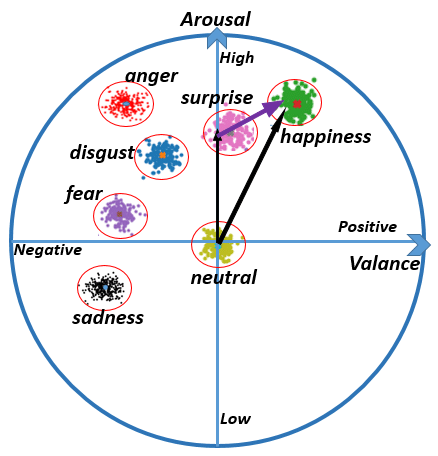
\includegraphics[width=.75\linewidth]{figs/2_state_of_the_art/emoValAro.png}
  \caption{The 2D Valence-Arousal model \cite{10.1007/11573548_51}.}
  \label{fig:emoValAro}
\end{subfigure}%
\begin{subfigure}{.5\textwidth}
  \centering
  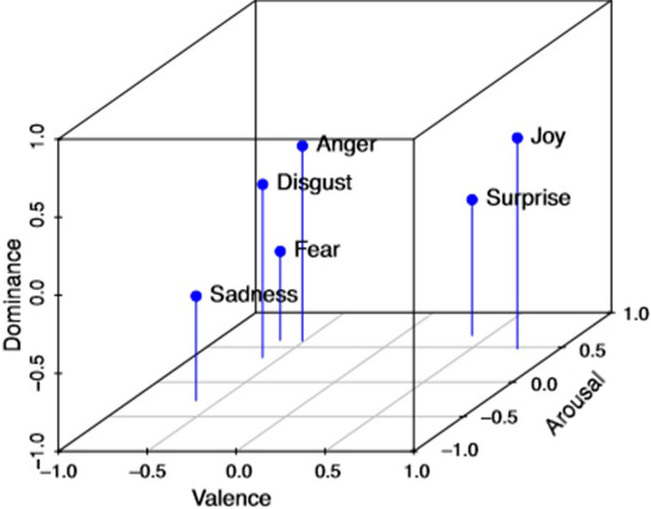
\includegraphics[width=\linewidth]{figs/2_state_of_the_art/VAD_Emotions.jpg}
  \caption{The 3D \acl{vad} model \cite{VAD_Emotions_article}.}
  \label{fig:emoVAD}
\end{subfigure}
\caption{Basic emotions spanned across different emotional models.}
\end{figure}


The arousal dimension refers to the level of energy or activation associated with an emotion, or in other words, the strength of the emotion. It measures whether humans are more or less likely to take some action under an emotional state.

The valence dimension measures how a human feels or the nature of the emotion, from positive to negative.

Also, a three-dimensional model may include a dimension of dominance or power, which refers to the seeming strength of the person, or the degree to which an individual feels in control or in charge of the situation that is causing the emotion, usually referred to as \ac{vad} model \cite{RUSSELL1977273}, displayed on figure \ref{fig:emoVAD}.


Dimensional representations of emotions are useful because they provide a wider range of describing an emotional state. Also, they are more suitable for quantifying variations over time, since changing successively from one discrete emotion to another may not make much sense in a real scenario. However, this model isn't as intuitive, therefore, it makes the distinction between a few basic emotions harder, such as surprise, since depending on the context it can have opposite values of valence \cite{Shuman2015}.

\section{Emotion Recognition Datasets}

The quality of the data affects the success of the recognition process. Incomplete, low-quality, or faulty data may lead to incorrect predictions; hence, data should be carefully designed and collected. 

When creating a database for emotion recognition research, researchers must consider factors such as the age, gender, and language of the speakers. Most databases include adult speakers, but there are also databases featuring children and elderly individuals. To improve the representativeness and usefulness of the database, researchers may also consider using different actors to express different emotions.

There are various databases containing emotional expressions in different languages. According to \citeauthor{Scherer2000ACI}, vocal emotion expressions may be driven by universal psychobiological mechanisms, as individuals from diverse cultures and speaking different languages can accurately recognize emotions expressed through speech better than would be expected by chance \cite{Scherer2000ACI}. This is supported by research demonstrating that even infants who cannot yet speak can recognize emotional cues in adult speech \cite{Slaney}. In another study, \citeauthor{Rajoo2016} investigated the influence of language on the ability of a \ac{ser} system, using spoken expressions of four selected emotions (anger, sad, happiness, and neutral) in three languages (Malay, English, and Mandarin). Their study revealed that there are language-specific differences in emotion recognition, with English showing a higher recognition rate compared to Malay and Mandarin. Additionally, the results support the conclusion that \ac{ser} is language-independent, but also suggest that emotions expressed by native speakers are more accurately recognized \cite{Rajoo2016}.

Databases for emotion recognition that can be used have three types:
\begin{itemize}
    \item \textbf{Acted}: recorded by professional or semi-professional actors in sound-proof studios;
    \item \textbf{Elicited}: created by, for example, placing speakers in a simulated emotional situation that can stimulate various emotions;
    \item \textbf{Natural}: mostly obtained from talk shows, call-center recordings, radio talks, and similar sources. Sometimes, these real-world speeches are referred to as spontaneous speech.
\end{itemize}

In video conferencing applications, the conversations take place in natural contexts, which is a fundamental factor to consider when choosing a dataset. Research has demonstrated that there are differences in the characteristics and accuracy of acted and genuine emotions \cite{Vogt}. Some studies have also suggested that simulated emotional speech may not be fully genuine and may be perceived more intensely than genuine emotional speech \cite{2041ade4b5294db59df9f67e9c854632}. Therefore, the studies on emotion recognition have shifted from focusing on induced expressions to spontaneous ones, but data on audiovisual expressions in natural contexts is still limited. Emotion expressions are infrequent, fleeting, and associated with complex contextual structures, making it difficult to collect a large amount of spontaneous data, as shown in a survey on audiovisual emotion recognition \cite{Wu2014}. Ostensibly, different types of databases are suitable for different purposes. For example, a database designed for mainly theoretical research may be more suitable in certain cases rather than one that is intended for use in a real-life industry application.

A summary of prominent datasets and their description is provided in the table \ref{datasets_overview}.

\begin{table}[h]
\caption{Summary and description of emotion recognition datasets.}
\centering
\label{datasets_overview}
\resizebox{\textwidth}{!}{%
\begin{tabular}{@{}lcccccc@{}}
\toprule
\multicolumn{1}{c}{Dataset} & Format & Language & Content & Emotions & Type\\
\midrule

\begin{tabular}[c]{@{}c@{}}EMO-DB \cite{Burkhardt2005}\end{tabular} &
  \begin{tabular}[c]{@{}c@{}}Audio\end{tabular} &
  \begin{tabular}[c]{@{}c@{}}German\end{tabular} &
  \begin{tabular}[c]{@{}c@{}}800 recording spoken\\by 10 actors (5 males\\and 5 females).\end{tabular} &
  \begin{tabular}[c]{@{}c@{}}7 emotions: anger, neutral,\\fear, boredom, happiness,\\sadness, disgust.\end{tabular} &
  \begin{tabular}[c]{@{}c@{}}Acted\end{tabular}\\

\begin{tabular}[c]{@{}c@{}}eNTERFACE’05 \cite{Martin2006}\end{tabular} &
  \begin{tabular}[c]{@{}c@{}}Audio\\Video\end{tabular} &
  \begin{tabular}[c]{@{}c@{}}English\end{tabular} &
  \begin{tabular}[c]{@{}c@{}}Videos by 42 subjects,\\coming from 14\\different nationalities.\end{tabular} &
  \begin{tabular}[c]{@{}c@{}}6 emotions: anger, fear,\\surprise, happiness,\\sadness and disgust.\end{tabular} &
  \begin{tabular}[c]{@{}c@{}}Elicited\end{tabular}\\

\begin{tabular}[c]{@{}c@{}}\acs{iemo} \cite{Busso2008}\end{tabular} &
  \begin{tabular}[c]{@{}c@{}}Audio\\Video\\Text\end{tabular} &
  \begin{tabular}[c]{@{}c@{}}English\end{tabular} &
  \begin{tabular}[c]{@{}c@{}}Conversations among\\pairs of 10
speakers\\(gender balanced)\\spanning 12 hours.\end{tabular} &
  \begin{tabular}[c]{@{}c@{}}10 categorical emotions\\\&  \acs{vad}\end{tabular} &
  \begin{tabular}[c]{@{}c@{}}Acted \&\\Elicited\end{tabular}\\

\begin{tabular}[c]{@{}c@{}}MOUD \cite{moud}\end{tabular} & 
  \begin{tabular}[c]{@{}c@{}}Audio\\Video\end{tabular} &
  \begin{tabular}[c]{@{}c@{}}Spanish\end{tabular} &
  \begin{tabular}[c]{@{}c@{}}80 product reviews\\YouTube videos.\end{tabular} &
  \begin{tabular}[c]{@{}c@{}}Positive, negative, or neutral\\sentiment.\end{tabular} &
  \begin{tabular}[c]{@{}c@{}}Natural\end{tabular}\\

\begin{tabular}[c]{@{}c@{}}CREMA-D \cite{Cao2014}\end{tabular} & 
  \begin{tabular}[c]{@{}c@{}}Audio\\Video\\Text\end{tabular} &
  \begin{tabular}[c]{@{}c@{}}English\end{tabular} &
  \begin{tabular}[c]{@{}c@{}}7442 clips of 12\\sentences spoken by 91\\actors (gender balanced).\end{tabular} &
  \begin{tabular}[c]{@{}c@{}}6 emotions: angry,\\disgusted, fearful, happy,\\neutral, and sad.\end{tabular} &
  \begin{tabular}[c]{@{}c@{}}Acted\end{tabular}\\
  
\begin{tabular}[c]{@{}c@{}}CMU-MOSI \cite{cmu-mosi}\end{tabular} &
  \begin{tabular}[c]{@{}c@{}}Audio\\Video\end{tabular} &
  \begin{tabular}[c]{@{}c@{}}English\end{tabular} &
  \begin{tabular}[c]{@{}c@{}}2199 movie reviews\\with annotated sentiment.\end{tabular} &
  \begin{tabular}[c]{@{}c@{}}Very negative to very positive\\in seven Likert steps.\end{tabular} &
  \begin{tabular}[c]{@{}c@{}}Natural\end{tabular}\\

\begin{tabular}[c]{@{}c@{}}MSP-Improv \cite{Busso2017}\end{tabular} &
  \begin{tabular}[c]{@{}c@{}}Audio\\Video\\Text\end{tabular} &
  \begin{tabular}[c]{@{}c@{}}English\end{tabular} &
  \begin{tabular}[c]{@{}c@{}}8438 recordings by\\12 actors.\end{tabular} &
  \begin{tabular}[c]{@{}c@{}}4 emotions: angry, sad,\\happy, neutral.\end{tabular} &
  \begin{tabular}[c]{@{}c@{}}Elicited\end{tabular}\\

\begin{tabular}[c]{@{}c@{}}CMU-MOSEI \cite{cmu-mosei}\end{tabular} &
  \begin{tabular}[c]{@{}c@{}}Audio\\Video\\Text\end{tabular} &
  \begin{tabular}[c]{@{}c@{}}English\end{tabular} &
  \begin{tabular}[c]{@{}c@{}}65 hours of YouTube videos\\from more than 1000\\speakers (gender balanced)\\and 250 topics.\end{tabular} &
  \begin{tabular}[c]{@{}c@{}}6 emotions: happiness,\\ sadness, anger, fear,\\disgust, surprise. Polarity\\in Likert scale.\end{tabular} &
  \begin{tabular}[c]{@{}c@{}}Natural\end{tabular}\\

\begin{tabular}[c]{@{}c@{}}MELD \cite{meld}\end{tabular} &
  \begin{tabular}[c]{@{}c@{}}Audio\\Video\\Text\end{tabular} &
  \begin{tabular}[c]{@{}c@{}}English\end{tabular} &
  \begin{tabular}[c]{@{}c@{}}1400 dialogues and 14000\\utterances from Friends\\TV series by multiple\\ speakers.\end{tabular} &
  \begin{tabular}[c]{@{}c@{}}7 emotions: Anger, disgust,\\sadness, joy, neutral, surprise\\and fear. Also positive,\\negative and neutral.\end{tabular} &
  \begin{tabular}[c]{@{}c@{}}Acted\end{tabular}\\
  
\begin{tabular}[c]{@{}c@{}}RAVDESS \cite{ravdess}\end{tabular} &
  \begin{tabular}[c]{@{}c@{}}Audio\\Video\end{tabular} &
  \begin{tabular}[c]{@{}c@{}}English\end{tabular} &
  \begin{tabular}[c]{@{}c@{}}7356 recordings\\by 24 actors with\\2 statements only.\end{tabular} &
  \begin{tabular}[c]{@{}c@{}}7 emotions: calm, happy,\\sad, angry, fearful,\\surprise, and disgust.\end{tabular} &
  \begin{tabular}[c]{@{}c@{}}Acted\end{tabular}\\

\begin{tabular}[c]{@{}c@{}}MSP-Podcast \cite{Lotfian2019}\end{tabular} &
  \begin{tabular}[c]{@{}c@{}}Audio\end{tabular} &
  \begin{tabular}[c]{@{}c@{}}English\end{tabular} &
  \begin{tabular}[c]{@{}c@{}}100 hours by\\over 100 speakers\end{tabular} &
  \begin{tabular}[c]{@{}c@{}}Activation, dominance and\\valence and 9\\categorical labels\end{tabular} &
  \begin{tabular}[c]{@{}c@{}}Natural\end{tabular}\\

\begin{tabular}[c]{@{}c@{}}TESS \cite{tess}\end{tabular} &
  \begin{tabular}[c]{@{}c@{}}Audio\end{tabular} &
  \begin{tabular}[c]{@{}c@{}}English\end{tabular} &
  \begin{tabular}[c]{@{}c@{}}2800 recording by\\2 actresses.\end{tabular} &
  \begin{tabular}[c]{@{}c@{}}7 emotions: anger, disgust,\\fear, happiness, pleasant\\surprise, sadness, and neutral.\end{tabular} &
  \begin{tabular}[c]{@{}c@{}}Acted\end{tabular}\\
  
\bottomrule
\end{tabular}%
} \end{table}

In a \citeyear{Jahangir2021} \ac{ser} \ac{sota} review article, \citeauthor{Jahangir2021} exhibited the most commonly used databases in their selected studies, figure \ref{fig:databases} \cite{Jahangir2021}. They realized the most popular ones had a gender-balanced number of speakers with high-quality recordings.

\begin{figure}[h]
  \centering
  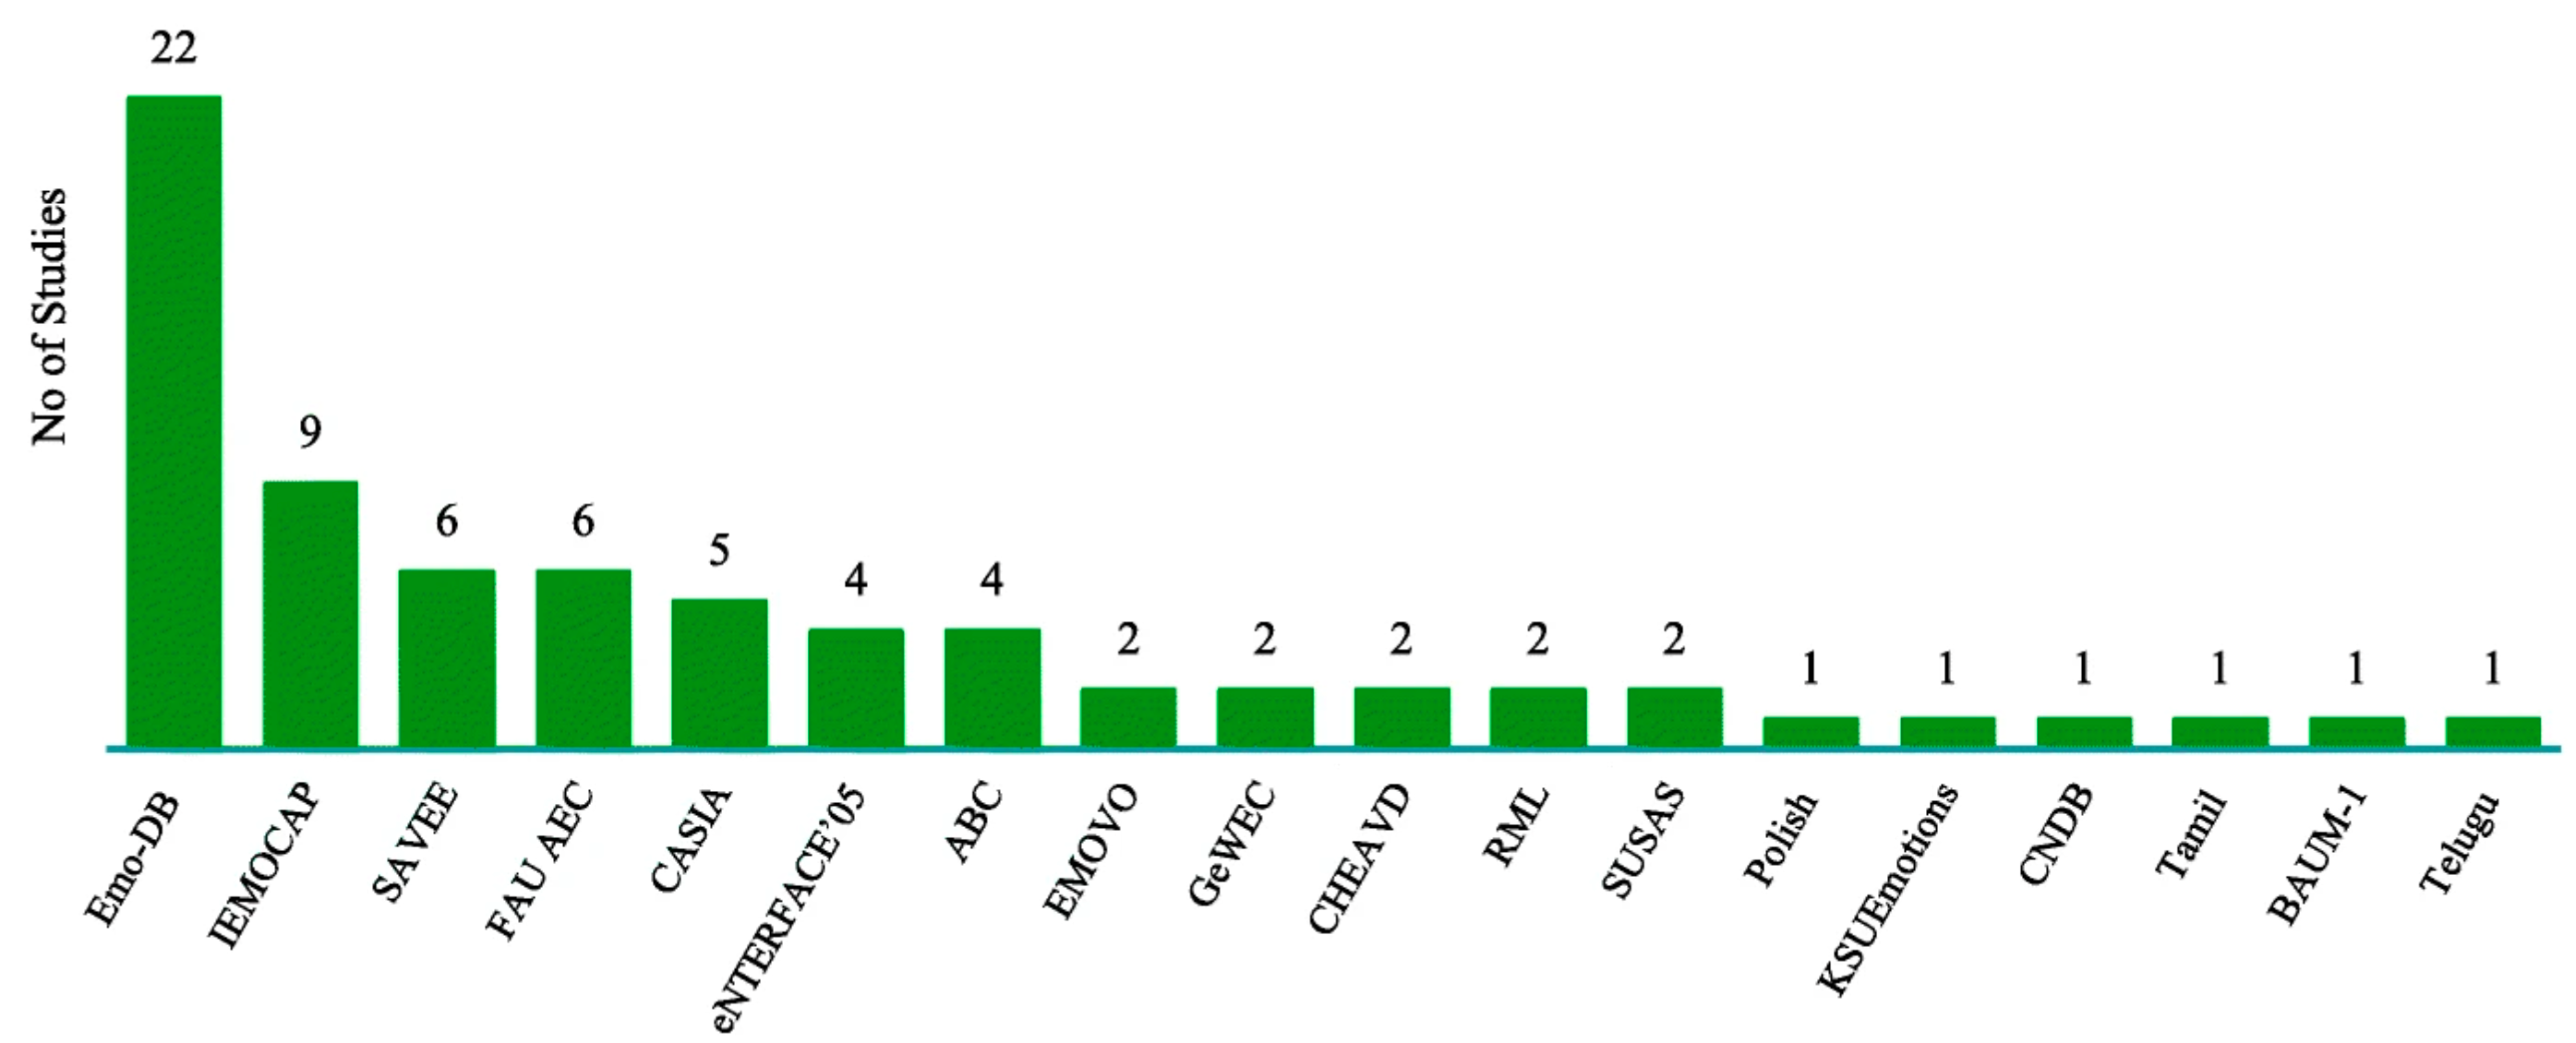
\includegraphics[width=\linewidth]{figs/2_state_of_the_art/sota.png}
  \caption{Frequency distribution of databases on reviewed articles from a \ac{sota} study \cite{Jahangir2021}.}
  \label{fig:databases}
\end{figure}

\section{\acl{ser}}

\ac{ser} is a subfield of artificial intelligence that focuses on the development of systems that can identify and classify the emotional state of a speaker based on their speech.

Speech is a vital tool for human communication and social interaction. Fundamentally, it is a continuous signal that can convey information, express emotions, and share meaning \cite{Narayanan2013}.

Words alone do not always transmit sufficient emotion, for instance, text messages can be easily misconceived. Hence, the necessity of \ac{ser} to aid and complete this task of figuring out the emotions/intent of human interaction. 

\subsection{Speech Features}

Speech features are characteristics of an audio signal that can be extracted and analyzed to understand its properties. These features are commonly categorized in the following three classes:
\begin{itemize}
    \item \textbf{Prosodic Features};
    \item \textbf{Spectral Features};
    \item \textbf{Voice Quality Features}.
\end{itemize}

Prosodic and spectral features are commonly employed in various fields, as they have been shown to effectively improve outcomes. By combining these features, it is possible to further optimize their usefulness and attain even better results.

Currently, there are a wide variety of acoustic properties that can be used to extract a large feature vector. Examples of these features include pitch, intensity, duration, and voice quality, which then several common statistics can be applied to them, such as minimum, mean, maximum, etc., as shown in table \ref{tab:features} adapted from a book \cite{Schuller2011}.


\begin{table}[h]
\centering
\caption{Overview on features commonly used for acoustic emotion recognition \cite{Schuller2011}.}
\label{tab:features}
\resizebox{\textwidth}{!}{%
\begin{tabular}{lllllll}
\hline
\multicolumn{1}{|l|}{\begin{tabular}[c]{@{}l@{}}\textbf{Intonation}\\ (F0 or pitch modelling)\end{tabular}} &
  \multicolumn{1}{l|}{} &
  \multicolumn{1}{l|}{} &
  \multicolumn{1}{l|}{} &
  \multicolumn{1}{l|}{\begin{tabular}[c]{@{}l@{}}\textbf{Extremes}\\ (min, max, range, ...)\end{tabular}} &
  \multicolumn{1}{l|}{} &
  \multicolumn{1}{l|}{} \\ \cline{1-1} \cline{5-5}
\multicolumn{1}{|l|}{\begin{tabular}[c]{@{}l@{}}\textbf{Intensity}\\ (energy, Teager, ...)\end{tabular}} &
  \multicolumn{1}{l|}{} &
  \multicolumn{1}{l|}{} &
  \multicolumn{1}{l|}{} &
  \multicolumn{1}{l|}{\begin{tabular}[c]{@{}l@{}}\textbf{Mean}\\ (arithmetic, absolute, ...)\end{tabular}} &
  \multicolumn{1}{l|}{} &
  \multicolumn{1}{l|}{} \\ \cline{1-1} \cline{5-5}
\multicolumn{1}{|l|}{\begin{tabular}[c]{@{}l@{}}\textbf{Linear Prediction}\\ (LPCC, PLP, ...)\end{tabular}} & \multicolumn{1}{l|}{\multirow{9}{*}{\begin{tabular}[c]{@{}l@{}}\textbf{Deriving}\\ (raw LLD, \\ deltas, \\ regression \\ coefficients, \\ LDA, \\ PCA, ...)\end{tabular}}} &
  \multicolumn{1}{l|}{\multirow{9}{*}{\begin{tabular}[c]{@{}l@{}}\textbf{Filtering}\\ (smoothing,\\ normalizing,\\ ...)\end{tabular}}} &
  \multicolumn{1}{l|}{\multirow{9}{*}{\begin{tabular}[c]{@{}l@{}}\textbf{Chunking}\\ (absolute,\\ relative,\\ ...)\end{tabular}}} &
  \multicolumn{1}{l|}{\begin{tabular}[c]{@{}l@{}}\textbf{Percentiles}\\ (quartiles, ranges, ...)\end{tabular}} & \multicolumn{1}{l|}{\multirow{9}{*}{\begin{tabular}[c]{@{}l@{}}\textbf{Deriving}\\ (raw LLD, \\ deltas, \\ regression \\ coefficients, \\ LDA, \\ PCA, ...)\end{tabular}}} &
  \multicolumn{1}{l|}{\multirow{9}{*}{\begin{tabular}[c]{@{}l@{}}\textbf{Filtering}\\ (smoothing,\\ normalizing,\\ ...)\end{tabular}}} \\ \cline{1-1} \cline{5-5}
\multicolumn{1}{|l|}{\begin{tabular}[c]{@{}l@{}}\textbf{Cepstral Coefficients}\\ (MFCC, ...)\end{tabular}} &
  \multicolumn{1}{l|}{} &
  \multicolumn{1}{l|}{} &
  \multicolumn{1}{l|}{} &
  \multicolumn{1}{l|}{\begin{tabular}[c]{@{}l@{}}\textbf{Higher Moments}\\ (std. dev., kurtosis, ...)\end{tabular}} &
  \multicolumn{1}{l|}{} &
  \multicolumn{1}{l|}{} \\ \cline{1-1} \cline{5-5}
\multicolumn{1}{|l|}{\begin{tabular}[c]{@{}l@{}}\textbf{Formants}\\ (amplitude, position, ...)\end{tabular}} &
  \multicolumn{1}{l|}{} &
  \multicolumn{1}{l|}{} &
  \multicolumn{1}{l|}{} &
  \multicolumn{1}{l|}{\begin{tabular}[c]{@{}l@{}}\textbf{Peaks}\\ (number, distances, ...)\end{tabular}} &
  \multicolumn{1}{l|}{} &
  \multicolumn{1}{l|}{} \\ \cline{1-1} \cline{5-5}
\multicolumn{1}{|l|}{\begin{tabular}[c]{@{}l@{}}\textbf{Spectrum}\\ (MFB, NMF, roll-off, ...)\end{tabular}} &
  \multicolumn{1}{l|}{} &
  \multicolumn{1}{l|}{} &
  \multicolumn{1}{l|}{} &
  \multicolumn{1}{l|}{\begin{tabular}[c]{@{}l@{}}\textbf{Segments}\\ (number, duration, ...)\end{tabular}} &
  \multicolumn{1}{l|}{} &
  \multicolumn{1}{l|}{} \\ \cline{1-1} \cline{5-5}
\multicolumn{1}{|l|}{\begin{tabular}[c]{@{}l@{}}\textbf{TF-Transformation}\\ (Wavelets, Gabor, ...)\end{tabular}} &
  \multicolumn{1}{l|}{} &
  \multicolumn{1}{l|}{} &
  \multicolumn{1}{l|}{} &
  \multicolumn{1}{l|}{\begin{tabular}[c]{@{}l@{}}\textbf{Regression}\\ (coefficients, error, ...)\end{tabular}} &
  \multicolumn{1}{l|}{} &
  \multicolumn{1}{l|}{} \\ \cline{1-1} \cline{5-5}
\multicolumn{1}{|l|}{\begin{tabular}[c]{@{}l@{}}\textbf{Harmonicity}\\ (HNR, spectral tilt, ...)\end{tabular}} &
  \multicolumn{1}{l|}{} &
  \multicolumn{1}{l|}{} &
  \multicolumn{1}{l|}{} &
  \multicolumn{1}{l|}{\begin{tabular}[c]{@{}l@{}}\textbf{Spectral}\\ (DCT coefficients, ...)\end{tabular}} &
  \multicolumn{1}{l|}{} &
  \multicolumn{1}{l|}{} \\ \cline{1-1} \cline{5-5}
\multicolumn{1}{|l|}{\begin{tabular}[c]{@{}l@{}}\textbf{Perturbation}\\ (jitter, shimmer, ...)\end{tabular}} &
  \multicolumn{1}{l|}{} &
  \multicolumn{1}{l|}{} &
  \multicolumn{1}{l|}{} &
  \multicolumn{1}{l|}{\begin{tabular}[c]{@{}l@{}}\textbf{Temporal}\\ (durations, positions,  ...)\end{tabular}} &
  \multicolumn{1}{l|}{} &
  \multicolumn{1}{l|}{} \\ \hline
  \\
\multicolumn{4}{l}{\textbf{Low-Level-Descriptors}} &
  \multicolumn{3}{l}{\textbf{Functionals}}
\end{tabular}%
}
\end{table}


\subsubsection{Prosodic Features}

Prosodic features are those that can be perceived by humans, such as intonation, rhythm, and loudness. The most widely used ones are based on \textbf{pitch}, \textbf{energy}, and \textbf{duration}.

Pitch, also known as the fundamental frequency or F0, refers to the lowest frequency of a periodic waveform. It is often used to convey emotion because it is influenced by the tension in the vocal folds and the sub-glottal air pressure. Studies have shown that the average pitch for males is typically about an octave lower than that of females, with an average pitch of 120 Hertz for males, 229 Hertz for females, and 155–185 Hertz for those with ambiguous gender. According to the study conducted by \citeauthor{ArputhaRathina2012} in \citeyear{ArputhaRathina2012}, there are clear differences in the pitch of the female and male genders when expressing different emotions. These differences may present a challenge for a gender-independent emotion classifier that relies solely on pitch \cite{ArputhaRathina2012}.

\begin{figure}[h]
  \centering
  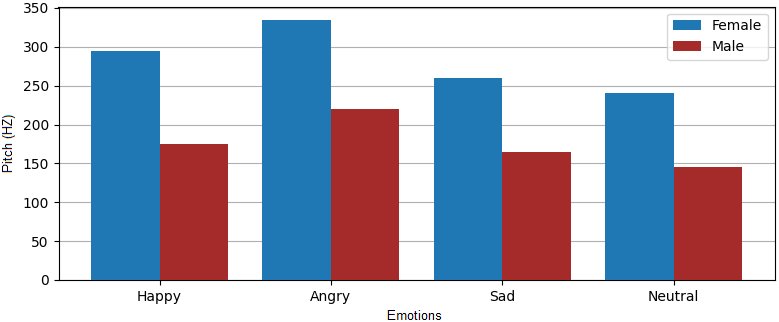
\includegraphics[width=.8\linewidth]{figs/2_state_of_the_art/Average-Pitch-Comparison-of-Male-and-Female-speak-ers.png}
  \caption{Average pitch comparison of male and female speakers’ \cite{ArputhaRathina2012}.}
  \label{fig:avgpitch}
\end{figure}

Prosodic features have been indicated as the most distinctive properties of emotional content for speech emotion recognition \cite{ZhihongZeng2009}.

\subsubsection{Spectral Features}

In the field of speech and audio processing, spectral features are used to analyze the characteristics of the human voice, which can convey information such as emotion, identity, and speaker traits.  The spectral content of speech signals varies significantly depending on the sounds being produced and the language being spoken, and it is often highly dynamic and time-varying.

One commonly used spectral feature is the \ac{mfccs}. \ac{mfccs} are calculated by performing a \ac{ft} on a window of audio data to obtain the spectral power, which is then mapped to the Mel-scale (a frequency scale that reflects how the human auditory system perceives sound). The Mel-scaled spectral power is then transformed into the cepstral domain using a discrete cosine transform, resulting in the \ac{mfccs} that represent the spectral power of the signal in the cepstral domain and can be used as input for tasks such as emotion recognition.

Another spectral feature is the gammatone frequency cepstral coefficient, which is similar to \ac{mfccs} in that they are derived using a \ac{ft} and a filter bank (in this case, a gammatone filter bank that models the auditory system's response to different frequencies). Linear prediction cepstral coefficients are another type of feature that is derived from the linear prediction of a signal. Log-frequency power coefficients are a type of feature that mimic the logarithmic filtering characteristics of the human auditory system and are obtained by measuring spectral band energies using a fast Fourier transform. 


\subsubsection{Voice Quality Features}

Voice quality is the set of characteristics that distinguish one person's voice from another. Some common methods for analyzing voice quality involve examining the physical properties of the vocal tract, such as jitter, shimmer, and the harmonics-to-noise ratio.

These properties may change involuntarily and can be used to differentiate emotions in the speech signal. Jitter refers to the variability in the period, or the time between successive peaks, of the fundamental frequency, whereas shimmer refers to the variability in the amplitude. Harmonics-to-noise ratio is a measure of the relative strength of the harmonics in a speech signal compared to the noise.

These three measures are often used together to assess the quality of a person's voice and can be useful in several tasks, e.g., treatment of voice disorders, age detection, speaker or emotion recognition, etc.

\subsection{Strategies}

The use case for this specific system of \ac{ser} is a video conferencing application where conversations are unpredictable, therefore, it is necessary to have a robust speech recognition system, however, some approaches can create privacy issues, for users who may not want to have their private conversations public, and even, ethical issues. Therefore, combining acoustic and linguistic content, by transcribing the speech to text, was not intended in this work, nonetheless, it is a remarkable approach that would potentially improve the system.

A \ac{ser} system requires a large and diverse dataset of speech samples, as well as feature extraction and preprocessing techniques to obtain relevant features from the audio signal, such as the ones mentioned above. Appropriate machine learning algorithms are then used to classify the emotional content of the speech based on the extracted features. In the past several years, classical machine learning algorithms, such as \ac{hmm} \cite{1220939}, \ac{svm}, and decision tree-based methods, have been utilized for audio sentiment analysis. More recently, researchers have proposed various neural network-based architectures to improve audio sentiment analysis. With the development of \ac{dl}, more complex neural-based architectures are proposed. For example, \ac{cnn}-based models have been used to train with the audio spectrograms or features derived from the signal.

Currently, there are two main types of implementations \cite{Zhao2018}:
\begin{itemize}
    \item \textbf{The traditional feature-based \ac{ser}}: hand-crafted features are extracted by applying a series of statistical aggregation functions to acoustic features of the audio signal, which are then passed on to a classifier;
    \item \textbf{Automatic feature extraction-based \ac{ser}}: avoids manual feature engineering and leverages the abilities of \ac{dl} techniques. This method typically involves using raw speech signals, Mel spectrograms, or \ac{mfccs} as input for a \ac{dnn} model.
\end{itemize}


\begin{figure}[h]
  \centering
  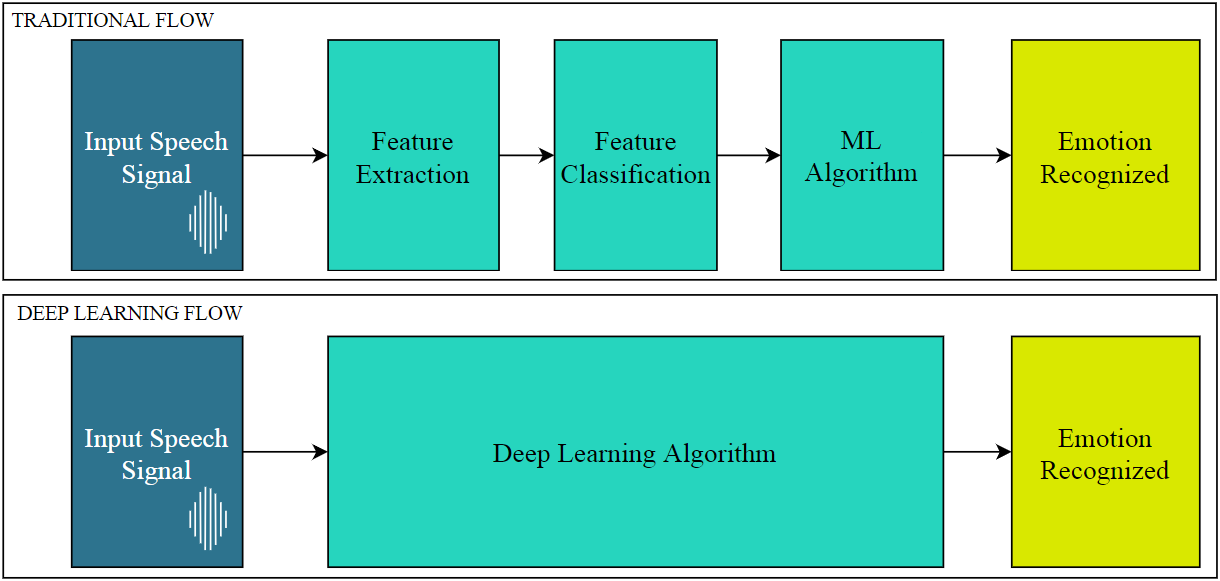
\includegraphics[width=\linewidth]{figs/2_state_of_the_art/methods.png}
  \caption{Traditional machine learning flow vs. automatic feature extraction with \ac{dl} flow \cite{Khalil2019}.}
  \label{fig:methods}
\end{figure}

Figure \ref{fig:methods}, displays the main difference between the methods, the traditional implementation has more steps, because it mainly depends on the feature extraction and selection processes. The \ac{dl} approaches avoid feature engineering and tend to improve recognition efficiency, however, it significantly increases complexity and the computational cost, which has a negative effect on \ac{ser} systems used in real-time scenarios.

\subsection{Traditional Feature-Based \ac{ser}}

The traditional feature-based \ac{ser} is a challenging task for researchers. It consists of applying a series of statistical aggregation functions (e.g., mean, max, variance, etc.) on acoustic features extracted from the speech to produce a statistical feature vector. The feature vector obtained can describe the temporal variations of speech signals, which are considered to be associated with the subjacent emotion. This vector is then analyzed, and feature selection is performed on it to reduce its size and reduce overfitting to the data, and finally, various classifiers are given that vector as input and are evaluated to find the most suitable for the task.

In \ac{sota} articles, the final set of selected features is often not the same across different studies. This selection of features for training classifiers has a significant impact on the overall performance of the \ac{ser} system, which is why it is a major challenge.

The statistical feature vector may contain only global features, extracted from the full-length utterance, or several local features, extracted from speech segments obtained from framing the utterance. The performance of the features based on their granularity is also analyzed in several studies.

\citeauthor{1202279} found that using global features (computed from gross statistics) resulted in a recognition rate of 86.6\% while using local features (computed from syllable duration, pitch, and energy values) resulted in a recognition rate of 77.6\%, while human judges had a recognition rate of 79.8\% \cite{1202279}. In a separate study, \citeauthor{Rao2012} observed that combining local and global prosodic features slightly improved performance compared to using only local features \cite{Rao2012}.


Forward methods and backward methods are two common techniques for feature selection. Forward methods begin with an empty (or very limited) feature set and add features incrementally. The most well-known forward method is the Sequential Forward Selection algorithm, which at each step tries adding each feature to the set and keeps the one that results in the highest improvement in accuracy.

\citeauthor{Luengo2005} (\citeyear{Luengo2005}) applied a Forward 3-Backward 1 wrapper method to select features. This method involves choosing the feature that maximizes accuracy in each step using leave-one-out testing. After three consecutive selections, the least useful feature is eliminated. Without feature selection, the authors obtained a recognition rate of 93.50\% with a \ac{svm} classifier and 84.79\% with a Gaussian Mixture Model using 86 prosodic features. However, by using the selected six best features, the recognition rates changed to 92.38\% and 86.71\%. In conclusion, it was noted that a slight reduction in recognition rate is compensated by a much lower computational cost of extracting and training the features.

In \citeyear{Gosztolya2015}, \citeauthor{Gosztolya2015} demonstrated that classification and regression algorithms can benefit from even simple feature selection techniques. They proposed a simple greedy forward-backward feature selection algorithm, which is less computationally costly than any other methods, for speech conflict intensity estimation, which significantly outperformed previous scores \cite{Gosztolya2015}.


\ac{cfs} is another popular method used in machine learning and data mining. \ac{cfs} involves calculating the correlation between each feature and the target variable, ranking the features based on their correlations, and selecting a subset of the highest-ranked features for use in a model. The goal of \ac{cfs} is to select a subset of features that are highly correlated with the target variable and not highly correlated with each other, to improve the performance of the model and reduce overfitting. In a study by \citeauthor{Schuller3D2011}, this method was applied to reduce the number of acoustic features from 760, for each of valence, activation, and dominance dimensions, to 238, 109, and 88, respectively, and improved their results by doing so \cite{Schuller3D2011}.

The \ac{gemaps} is a set of features used in speech emotion recognition developed by researchers at the University of Geneva \cite{Eyben2016}. It is designed to be a compact and efficient feature set for automatic emotion recognition from speech. It includes a range of prosodic and acoustic features that are relevant to emotion recognition, such as pitch, intensity, spectral properties, and temporal features. \ac{gemaps} feature set has been utilized in several studies on speech emotion recognition, e.g., \cite{Tarantino2019}, as well as in applications such as affective computing, virtual assistants, and human-computer interaction.

Many of the early researchers used traditional machine learning classification techniques such as Linear Discriminant Analysis, Regular Discriminant Analysis, \ac{svm}, K-Nearest Neighbors, Random Forests, and Gaussian Mixture Models \cite{Kuchibhotla2014}. Moreover, ensemble learning has also been employed by researchers to combine the predictions of multiple individual classifiers to improve performance.

\citeauthor{Albornoz2011} built a hierarchical classifier with two stages, on each stage they predicted different emotions using a different set of features and classifiers \cite{Albornoz2011}. They showed that 12 mean \ac{mfccs} features, deltas, and acceleration coefficients are the best features for the first stage with a \ac{hmm} with 30 Gaussians in the mixture classifier. For the second stage with a \ac{hmm}, they obtained as the best features, 12 means \acp{mfccs}, 30 means log-spectrum, and mean and standard deviation pitch. Using the EMO-DB corpus, they achieved an accuracy of 71.75\%.

In a study, \citeauthor{Lee2011} (\citeyear{Lee2011}) used a traditional strategy to extract 16 low-level descriptors from audio data, including zero crossing rate, root-mean-square energy, pitch, harmonics-to-noise ratio, and 12 \ac{mfccs} and deltas. They then applied 12 different statistical functions, resulting in a set of 384 acoustic features per utterance. The researchers used a multi-level binary decision tree structure with different classifiers at each level to classify the data by dividing the problem into sub-problems. For example, at the first level, they compared the "neutral" label to all other labels. This approach resulted in an \ac{uar} of 41.57\% on the AIBO dataset and 58.46\% on the \ac{iemo} dataset \cite{Lee2011}, with 5 and 4 classes respectively.

In \citeyear{HandCraftedSahu}, \citeauthor{HandCraftedSahu} developed a set of hand-crafted features for an audio signal using the \ac{iemo} dataset. The authors obtained an eight-dimensional vector by applying statistical functions 
 to acoustic features such as pitch, harmonics, and pause \cite{HandCraftedSahu}. They also found that ensembling models improved performance, and they achieved a maximum accuracy of 56.6\% with a model that combined random forest, extreme gradient boosting, and a multilayer perceptron.


\subsection{\acl{dl}-Based \ac{ser}}

As \ac{dl} technology has advanced, automatic feature learning algorithms have become increasingly popular for \ac{ser}, and even in other areas, for example, in cardiac spectrogram analysis, it is one of the state-of-art approaches, \cite{8759878} and \cite{Zhou2022}, in which the spectrogram of the audio from the heartbeat is used to evaluate the cardiac activity. These algorithms are effective at learning task-specific features without the need for extensive manual feature engineering.

\ac{dnn} techniques for \ac{ser} are primarily trained using raw signals, spectrograms, low-level descriptors, and \ac{mfccs}, which have been shown to produce satisfactory results. Various \ac{dnn} architectures including \ac{rnn}, \ac{lstm}, and attention-based convolution \ac{rnn} have been designed for \ac{ser}, each with its strengths and weaknesses. \acp{cnn} and their variations are the most common, as they are known for their ability to extract a large number of hidden features from signals and images.

A new architecture was introduced in \citeyear{Issa2020} by \citeauthor{Issa2020}, for identifying emotions in sound files using a one-dimensional \ac{cnn}. They obtain a one-dimensional array by taking mean values along the time axis of various features, including \ac{mfccs}, chromagram, Mel spectrogram, Tonnetz representation, and spectral contrast, from the sound files and use them as inputs for the \ac{cnn}. The proposed framework was evaluated using samples from the RAVDESS, EMO-DB, and \ac{iemo} datasets. The framework achieved accuracies of 71.61\% for RAVDESS (with 8 emotions), 86.1\% for EMO-DB (with 7 emotions), 95.71\% for EMO-DB (with 7 emotions), and 64.3\% for \ac{iemo} (with 4 emotions) in speaker-independent audio classification tasks \cite{Issa2020}.

It is important to note that the way the information contained in an audio spectrogram is used can be different, as some authors use three channels of the spectrogram, such as the RGB of the plotted image, or even using the static, delta, and delta-deltas of it, essentially having a 3-D tensor, while other authors use a 2-D tensor with the spectrogram values.

In a paper published in \citeyear{GARCIAORDAS2021102946}, \citeauthor{GARCIAORDAS2021102946} proposed a fully \ac{cnn} that can process variable input lengths for near real-time sentiment analysis \cite{GARCIAORDAS2021102946}. The use of \acp{mfccs} made it easier to identify emotions in audio signals. The model achieved superior performance compared to other machine learning models on the EmoDB, RAVDESS, and TESS datasets, with accuracies of 75.28\%, 92.71\%, and 99.03\%, respectively.

The use of \acp{cnn} and \acp{rnn} increased in recent years, driven by their successes in various applications, and researchers have begun exploring the potential benefits of combining these models into a single architecture. For example, in a previous study, \citeauthor{ma18b_interspeech} (\citeyear{ma18b_interspeech}) proposed a neural network architecture designed specifically to handle variable-length speech by combining \ac{cnn}-based deep spectrogram representations with a \ac{rnn} to process variable-length speech segments. Their model achieved a weighted and unweighted accuracy of 71.4\% and 64.22\% on the \ac{iemo} dataset \cite{ma18b_interspeech}. In another study that used the same corpus, \citeauthor{Zhao2019} (\citeyear{Zhao2019}) developed an attention-based bidirectional \ac{lstm} \ac{rnn} with attention-based fully convolutional networks and achieved weighted and unweighted accuracies of 68.1\% and 67.0\% \cite{Zhao2019}.

\citeauthor{Luo2018} in \citeyear{Luo2018}, proposed a model for audio sentiment analysis that combines multiple traditional acoustic features and spectrum graphs. The authors analyze the \ac{mfccs}, spectral centroid, chroma-short-time \ac{ft}, and spectral contrast. The best model used is a combination of a \ac{lstm} network and a \ac{cnn}. The model was tested on the CMU-MOSI and MOUD datasets, achieving accuracies of 68.74\% and 69.64\% for 4 and 2 emotion classes, respectively.

In \citeyear{8421023}, \citeauthor{8421023} proposed a 3-D attention-based convolutional \ac{rnn}, which learns discriminative features from the input data. The input to the model is a Mel spectrogram with static, deltas, and delta-deltas, which is processed by a 3-D \ac{cnn} and then combined with a \ac{lstm} for high-level feature extraction. To address silent and emotion-irrelevant frames, an additional attention model is used to focus on emotion-relevant frames and produce discriminative utterance-level features. Their proposed method achieved \ac{sota} performance on the \ac{iemo} and Emo-DB corpora, with \acp{uar} of 64.74±5.44\% and 82.82±4.99\% \cite{8421023}, using a 10-fold cross-validation technique.

In a paper published by \citeauthor{Muppidi2021}, the authors proposed one of the first quaternion-based \ac{cnn} for \ac{ser}. Their model is significantly smaller than other \ac{dl} models and achieved \ac{sota} results in terms of accuracy on several datasets, including RAVDESS (77.67\% accuracy with 8 emotions), \ac{iemo} (70.46\% accuracy with 4 emotions), and EMO-DB (88.78\% accuracy with 7 emotions) \cite{Muppidi2021}.


\subsubsection{Transfer Learning}

Transfer learning is a machine learning technique that involves using the knowledge gained from training a model on one task to improve the performance of a model on a related task.

As stated before, finding a large amount of labeled data to train a \ac{ser} system can be challenging. That is why leveraging the knowledge gained from training a model on a large dataset of speech samples can be particularly useful to reduce the amount of data and computational cost required.

Although there is a significant difference between audio signals and spectrograms and standard ImageNet images, the principles of transfer learning still apply. In a \citeyear{rethinkPalanisamy} paper, \citeauthor{rethinkPalanisamy} demonstrated this by using pre-trained weights from image classification models led to improved performance compared to using randomly initialized weights. Their ensemble of models pre-trained on ImageNet achieved \ac{sota} results on the ESC-50 and UrbanSound8K datasets \cite{rethinkPalanisamy}.

It is also common to extract features from the spectrogram images using pre-trained models and use them as input to more traditional machine learning models, as shown in a study by \citeauthor{8085174}, that used the pre-trained \ac{cnn} AlexNet model to learn deep features and feed them to a \ac{svm} \cite{8085174}.

In table \ref{tab:article_overview} we provide a list of our reviewed articles for both strategies commonly used in audio classification tasks, and, subsequently, \ac{ser} tasks.

\begin{table}[h]
\centering
\caption{Overview of audio classification articles with strategies.}
\label{tab:article_overview}
\resizebox{\textwidth}{!}{%
\begin{tabular}{@{}lcccc@{}}
\toprule
  Paper Title (Publication Date) &
  Audio Features &
  Classifier &
  \begin{tabular}[c]{@{}c@{}}Datasets (N\textsuperscript{\underline{o}} of Labels)\\\& Accuracies (\%)\end{tabular}\\ 
  
  \midrule
  \multicolumn{4}{c}{Traditional Feature-Based Approaches} \\
  \midrule

  \begin{tabular}[c]{@{}c@{}}Spoken emotion recognition\\using hierarchical\\classifiers (\citedate{Albornoz2011}) \cite{Albornoz2011}\end{tabular} &
  \begin{tabular}[c]{@{}c@{}}\ac{mfccs}\\Log-spectrum\\Pitch\end{tabular} &
  \begin{tabular}[c]{@{}c@{}}\ac{hmm}\end{tabular} &
  \begin{tabular}[c]{@{}c@{}}EMO-DB (7): 71.75\end{tabular} \\
    
  \begin{tabular}[c]{@{}c@{}}Emotion recognition\\using a hierarchical\\binary decision\\tree approach\\(\citedate{Lee2011}) \cite{Lee2011}\end{tabular} &
  \begin{tabular}[c]{@{}c@{}}Zero crossing rate\\Root-mean-square energy\\Pitch\\\ac{mfccs}\\Harmonics-to-noise ratio\end{tabular} &
  \begin{tabular}[c]{@{}c@{}}Multi-level binary\\decision trees\end{tabular} &
  \begin{tabular}[c]{@{}c@{}}(\acp{uar})\\AIBO (5): 41.57\\\ac{iemo} (4): 58.46\end{tabular} \\

  \begin{tabular}[c]{@{}c@{}}Multimodal \ac{ser}\\and Ambiguity\\Resolution (\citedate{HandCraftedSahu}) \cite{HandCraftedSahu}\end{tabular} &
  \begin{tabular}[c]{@{}c@{}}Pitch\\Harmonics\\Pause\end{tabular} &
  \begin{tabular}[c]{@{}c@{}}Random forest, extreme\\gradient boosting and\\multilayer perceptron\end{tabular} &
  \begin{tabular}[c]{@{}c@{}}\ac{iemo} (4): 56.6\end{tabular} \\

  \midrule
  \multicolumn{4}{c}{\acl{dl}-Based Approaches} \\
  \midrule

  \begin{tabular}[c]{@{}c@{}}\ac{ser} with deep \acp{cnn}\\(\citedate{Issa2020}) \cite{Issa2020}\end{tabular} &
  \begin{tabular}[c]{@{}c@{}}\ac{mfccs}\\Chromagram\\Mel spectrogram\\Spectral contrast\end{tabular} &
  \begin{tabular}[c]{@{}c@{}}One-dimensional\\\ac{cnn}\end{tabular} &
  \begin{tabular}[c]{@{}c@{}}RAVDESS (8): 71.61\\ \ac{iemo} (4): 64.30\\ EMO-DB (7): 86.10\end{tabular} \\

 \begin{tabular}[c]{@{}c@{}}Sentiment analysis in\\non-fixed length audios\\using a Fully \ac{cnn} (\citedate{GARCIAORDAS2021102946}) \cite{GARCIAORDAS2021102946}\end{tabular} &
  \begin{tabular}[c]{@{}c@{}}Mel-Spectrogram\\\ac{mfccs}\end{tabular} &
  \begin{tabular}[c]{@{}c@{}}Fully \ac{cnn}\end{tabular} &
  \begin{tabular}[c]{@{}c@{}}RAVDESS (8): 75.28\\EMO-DB (7): 92.71\\TESS: 99.03\end{tabular} \\

  \begin{tabular}[c]{@{}c@{}}Emotion Recognition from\\Variable-Length Speech\\Segments Using \ac{dl}\\on Spectrograms (\citedate{ma18b_interspeech}) \cite{ma18b_interspeech}\end{tabular} &
  \begin{tabular}[c]{@{}c@{}}Log-Spectrograms\end{tabular} &
  \begin{tabular}[c]{@{}c@{}}\ac{cnn} and \ac{rnn}\end{tabular} &
  \begin{tabular}[c]{@{}c@{}}\ac{iemo} (4): 64.22\end{tabular} \\

  \begin{tabular}[c]{@{}c@{}}Exploring Deep\\Spectrum Representations\\via
Attention-Based \ac{rnn}\\and \ac{cnn} for \ac{ser}\\(\citedate{Zhao2019}) \cite{Zhao2019} \end{tabular}&
  \begin{tabular}[c]{@{}c@{}}Mel-Spectrogram\end{tabular} &
  \begin{tabular}[c]{@{}c@{}}Attention-based\\bidirectional \ac{lstm}\\and fully \ac{cnn}\end{tabular} &
  \begin{tabular}[c]{@{}c@{}}\ac{iemo} (4): 67.0\end{tabular} \\
  
  \begin{tabular}[c]{@{}c@{}}Audio Sentiment Analysis\\by Heterogeneous Signal\\Features Learned from\\Utterance-Based Parallel\\Neural Network (\citeyear{Luo2018}) \cite{Luo2018}\end{tabular}&
  \begin{tabular}[c]{@{}c@{}}\ac{mfccs}\\Spectral centroid\\Spectral contrast\\Chromagram \end{tabular} &
  \begin{tabular}[c]{@{}c@{}}\ac{lstm} and \ac{cnn}\end{tabular} &
  \begin{tabular}[c]{@{}c@{}}MOSI (4): 68.74\\MOUD (2): 69.64\end{tabular} \\
  
  \begin{tabular}[c]{@{}c@{}}3-D Convolutional\\\ac{rnn} With Attention\\Model for \ac{ser} (\citedate{8421023}) \cite{8421023}\end{tabular}&
  \begin{tabular}[c]{@{}c@{}}Mel spectrogram\end{tabular} &
  \begin{tabular}[c]{@{}c@{}}3-D attention-based\\convolutional \ac{rnn}\end{tabular} &
  \begin{tabular}[c]{@{}c@{}}(\acp{uar})\\\ac{iemo} (4): 64.74\\EMO-DB (7): 82.82\end{tabular} \\
 
\begin{tabular}[c]{@{}c@{}}\ac{ser} Using\\Quaternion \ac{cnn}\\
(\citedate{Muppidi2021}) \cite{Muppidi2021}\end{tabular}&
  \begin{tabular}[c]{@{}c@{}}Mel spectrogram\\ encoded in an RGB\\quaternion domain\end{tabular} &
  \begin{tabular}[c]{@{}c@{}}Quaternion \ac{cnn}\end{tabular} &
  \begin{tabular}[c]{@{}c@{}}RAVDESS (8): 77.87\\ \ac{iemo} (4): 70.46\\ EMO-DB (7): 88.78\end{tabular} \\

  \begin{tabular}[c]{@{}c@{}}Rethinking \ac{cnn}\\Models for Audio\\Classification (\citedate{rethinkPalanisamy}) \cite{rethinkPalanisamy}\end{tabular}&
  \begin{tabular}[c]{@{}c@{}}Mel spectrogram\end{tabular} &
  \begin{tabular}[c]{@{}c@{}}Ensemble of\\ImageNet pre-trained\\DenseNets\end{tabular} &
  \begin{tabular}[c]{@{}c@{}}ESC-50 (50): 92.89\\UrbanSound8K (10):  87.42\end{tabular} \\

  \begin{tabular}[c]{@{}c@{}}\ac{ser} Using Deep \ac{cnn}\\and Discriminant\\
Temporal Pyramid\\Matching (\citedate{8085174}) \cite{8085174} \end{tabular}&
  \begin{tabular}[c]{@{}c@{}}Mel spectrogram\end{tabular} &
  \begin{tabular}[c]{@{}c@{}}Deep \ac{cnn}\\(Fine-tuned the\\AlexNet pre-trained\\on ImageNet)\end{tabular} &
  \begin{tabular}[c]{@{}c@{}}EMO-DB (7): 87.31\\RML (6): 69.70\\eNTERFACE05 (6): 76.56\\BAUM-1s (6): 44.61\end{tabular} \\

\bottomrule
\end{tabular}%
}
\end{table}


\section{Multimodal Emotion Recognition}

There are several strategies to capture features for recognizing emotions. Multimodality, which refers to the use of multiple channels of information, is exploited to improve the accuracy of \ac{ser} systems. By combining multiple modalities, such as speech, facial expressions, and speech transcriptions, as the figure \ref{fig:multimodal} demonstrates, or even electrocardiogram readings \cite{Hasnul2021}, many researchers have been able to achieve improved results. However, multimodality increases complexity, since it becomes necessary to fuse the information across modalities in some way that achieves accurate emotional predictions.

\begin{figure}[h]
  \centering
  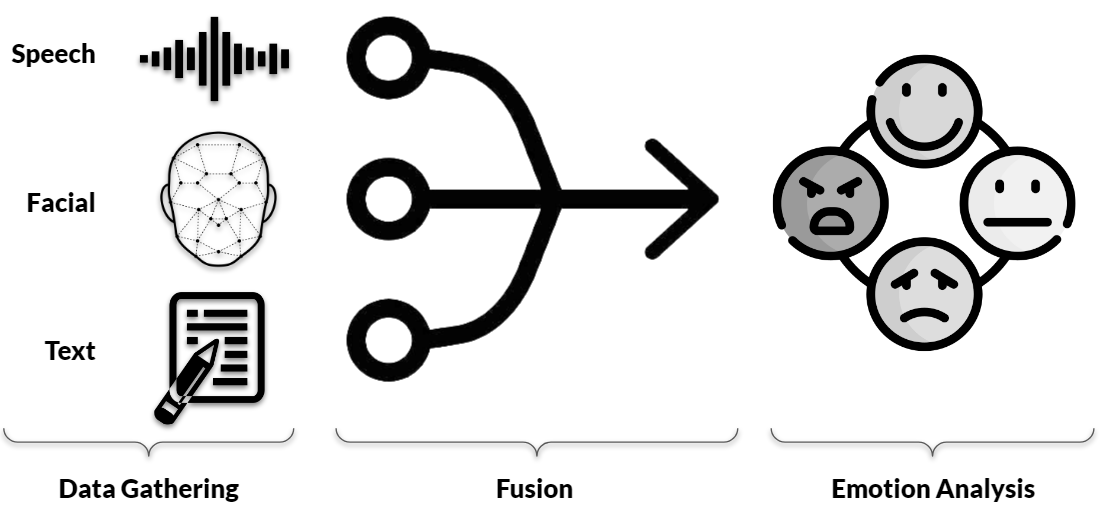
\includegraphics[width=.8\linewidth]{figs/2_state_of_the_art/multimodality.png}
  \caption{Multimodal emotion recognition illustration.}
  \label{fig:multimodal}
\end{figure}

Four main methods of fusion can be used in multimodal systems:
\begin{itemize}
\item \textbf{Feature level}: This involves combining the features of different modalities and creating a new, high-dimensional feature set.

\item \textbf{Decision level}: Each feature set from different modalities is given as input to different classifiers, and then the prediction results are combined.

\item \textbf{Model level}: The goal of this method is to build a model that captures the complex relationships among the different modalities.

\item \textbf{Hybrid}: This approach combines and takes advantage of the different fusion methods.

\end{itemize}

One of the strategies is to use speech transcriptions to understand the context of the utterances correctly and predict their intent. Human oral communication consists of both linguistic and acoustic content, any subtle change in these cues can alter the significance of an expression. However, this approach alone tends to fail, word meanings are very ambiguous, and it fails to capture some low-level features of the speech itself, therefore not achieving the best results. Thus, emotion and sentiment recognition could benefit from considering both linguistic and acoustic features. \citeauthor{BHASKAR2015635} evidenced this improvement by using a hybrid approach based on text and speech mining \cite{BHASKAR2015635}. Similarly, \citeauthor{ser_strategies} also corroborated this idea by using a model that fuses \ac{mfccs} indicators with text transcriptions to predict emotions \cite{ser_strategies}.

In a paper published in \citeyear{Lu2020} by \citeauthor{Lu2020}, it was used a pre-trained end-to-end automatic speech recognition model to extract text features from audio data and combined them with other acoustic features. These features were then fed into a \ac{rnn} with multi-head self-attention, which improved the accuracy of sentiment analysis using only audio data from 67.4\% to 71.7\% on the \ac{iemo} dataset.

In a study by \citeauthor{Handa2021} (\citeyear{Handa2021}), a model was proposed for fusing facial and speech features using a \ac{svm}. The model employed an AlexNet and a deep \ac{lstm} network to extract the facial and speech features, respectively, which were then combined and fed into the \ac{svm} for classification. The model achieved \ac{sota} results on the eNTERFACE’05 dataset for classifying seven emotions, with an overall accuracy of 76.61\% \cite{Handa2021}.

\citeauthor{Yan2021} in \citeyear{Yan2021}, proposed a multi-tensor fusion network with cross-modal modeling with video, audio, and text cues for emotion recognition \cite{Yan2021}. To perform their classification experiences, and obtained results that outperformed their current \ac{sota}, achieving an F1 score of 81.0\% and 81.3\% on the CMU-MOSI and the CMU-MOSEI datasets, respectively.

\section{Emotion Recognition Services}

The widespread use of video conferencing applications has increased significantly during the COVID-19 pandemic, as many people have been forced to communicate remotely. These systems typically use audio and video inputs, as well as text input, to facilitate communication. This growth of video conference usage increased the demand for tools that can improve the virtual communication experience.

In the customer service industry, video conferencing has become very popular, but it can be a challenging task, such as dealing with agitated customers. By providing real-time feedback on the emotions of participants, emotion recognition technologies can prevent problematic situations and evaluate the effectiveness and engagement of the customer service experience.

\citeauthor{Buitelaar2018} in \citeyear{Buitelaar2018} summarized some other known emotion recognition services, that are helping to advance the field, along with their characteristics, displayed below in the table \ref{table:emoServices}. It is visible that most of the services at the time of this study are paid and not open-source \cite{Buitelaar2018}.

\begin{table}[h]
\centering
\caption{Emotion recognition services for facial, textural, and speech contents \cite{Buitelaar2018}.}
\label{table:emoServices}
\resizebox{.85\textwidth}{!}{%
\begin{tabular}{@{}lccc@{}}
\toprule
Service & Modality & Open-Source & Free\\
\midrule

\begin{tabular}{@{}l@{}}IBM Watson Alchemy Language \cite{ibmwatson}\\Bitext \cite{bitext2022}\end{tabular} & Text & No & No \\

\begin{tabular}{@{}l@{}}Synesketch \cite{Krcadinac2016}\end{tabular} & Text & Yes & Yes \\

\begin{tabular}{@{}l@{}}Microsoft Cognitive Services \cite{microsoftservice}\\IMOTIONS \cite{kristensen2022}\end{tabular} & Facial & No & No \\

\begin{tabular}{@{}l@{}}Affectiva Emotion API \cite{affectiva}\end{tabular} & Facial & No & Free/Enterprise Editions \\

\begin{tabular}{@{}l@{}}EmoVu \cite{emovuservice}\end{tabular} & Facial & No & No \\

\begin{tabular}{@{}l@{}}Nviso \cite{humanbeaviourservice}\\SkyBiometry \cite{skybiometry2022}\end{tabular} & Facial & No & Limited/Non-Free Editions \\

\begin{tabular}{@{}l@{}}audEERING SensAI \cite{audeering2022}\end{tabular} & Speech & Yes & Free Research Edition \\

\begin{tabular}{@{}l@{}}Good Vibrations \cite{goodvibrations}\end{tabular} & Speech & No & No \\

\begin{tabular}{@{}l@{}}Vokaturi \cite{Vokaturi}\end{tabular} & Speech & No & Limited/Enterprise Editions \\
  
\bottomrule
\end{tabular}%
}
\end{table}


More recently, companies have been working on developing technology for recognizing human emotions, and they are, gradually, adding multimodality to perform emotion analysis. Affectiva \cite{affectiva}, has added the audio modality to their emotion recognition system that initially was only with facial cues. The company primarily uses its technology for market research, but it has also been applied in the automotive industry to monitor drivers' emotions and cognitive states. Microsoft \cite{microsoftservice} has also integrated into their emotion API other modalities over time, such as text and speech. EmoVoice \cite{Wagner13}, is another framework that uses acoustic features of speech to recognize human behavior in real-time, without the need for speech transcription.


\section{Software Tools}

For working and manipulating speech data and also machine learning techniques, different software tools are necessary. Generally, \textbf{Python} \cite{van1995python}, is the most widely used programming language in all machine learning-related tasks, along with \textbf{Pip} \cite{pypi} to install external resources, labeled as Python libraries. Important Python libraries in this area are \textbf{Numpy} \cite{2020NumPyArray} and \textbf{Pandas} \cite{mckinney2010data}, which provide high-level mathematical functions for dealing with big vectors and matrices, \textbf{Matplotlib} \cite{hunter2007matplotlib} and \textbf{Seaborn} \cite{michael_waskom_2017_883859}, for statistical data visualization, \textbf{Keras} \cite{gulli2017deep} and \textbf{scikit-learn} \cite{pedregosa2011scikit}, for implementing and manipulating machine learning algorithms.

For extracting and processing speech, there are several tools available in Python, such as:
\begin{itemize}
    \item \textbf{Librosa} \cite{Librosa}: provides tools for music and audio analysis. It helps to visualize audio signals and extract features using signal processing techniques;
    \item \textbf{OpenSmile} \cite{Eyben2010}: open-source toolkit for audio analysis, processing, and classification that focuses on speech and music applications;
    \item \textbf{COVAREP} \cite{Degottex2014}: an open-source repository of advanced speech processing algorithms that are useful for tasks such as speech analysis, synthesis, and conversion;
    \item \textbf{Spafe} \cite{spafe}: simplifies the process of extracting features from mono audio files and includes various filter bank modules and other spectral statistics;
    \item \textbf{Pydiogment} \cite{ayoubmalek2020}: makes it easy to augment audio files by generating multiple versions with different speeds, tones, and other modifications;
    \item \textbf{Noise Reduce} \cite{tim_sainburg_2019_3243139,sainburg2020finding}: helps to remove noise from time-based signals such as speech.
\end{itemize}

Frequently, \ac{vad*} algorithms are employed in speech processing systems. These algorithms are designed to be highly accurate and efficient in detecting when a user is speaking and filtering out background noise and other non-speech signals. Examples of \ac{vad*} toolkits are:

\begin{itemize}
    \item \textbf{Silero} \cite{SileroVAD}: intended to be used in real-time speech processing applications, it is optimized for performance on a wide range of devices, including mobile phones and other embedded systems;

    \item \textbf{Py-webrtcvad} \cite{WebRTCVad}: python interface to the Google's WebRTC \ac{vad*} project, which is an open-source project that provides web browsers and mobile applications with real-time communication capabilities.
\end{itemize}


\section{Summary}

Through the \ac{sota} research, it is possible to state the significant progress over time of not only \ac{ser}, but emotion recognition systems in general. Here are a few key takeaways that emerged from it:

\begin{itemize}
    \item Due to the subjectivity of emotions, the lack of consensus on how to label them, and the need for a large and diverse emotional corpus (e.g. different contexts, genders, languages, etc.), makes the whole process of creating and evaluating an emotion recognition system a very challenging task.

    \item Audio feature engineering is a critical aspect of \ac{ser} due to the large variety of features available and the need to carefully select them, including prosodic, spectral, and voice quality features.

    \item Traditional feature-based approaches use more classical models and focus mainly on feature selection methods.

    \item \ac{dl} strategies with automatic feature extraction capabilities have, in general, outperformed the traditional acoustic feature extraction approach. The most popular models for this are \ac{cnn}, \ac{rnn} (\ac{lstm}), and hybrid \ac{cnn}-\ac{rnn} architectures, with Mel spectrogram as input for them.

    \item The field of affective computing, which originally focused mainly on using facial cues to recognize emotions, has seen success in using multiple channels of information (multimodality). This shift has allowed for more accurate emotion recognition, and many current solutions in the market are taking advantage of this approach.

    \item There are still areas in which emotion recognition systems need to be improved, such as being able to handle a wider range of input signals and increase reliability. For example, most systems overlook the case of input channels with noise, where the system should weigh each differently, and also, research for online classification contexts is still underdeveloped.

\end{itemize}

Overall, there is a significant amount of ongoing research and development that is taking place on emotion recognition systems and has successfully advanced further their capability and reliability, however, there remain a lot of limitations to overcome and areas to improve.

%\chapter{Methodology}
\label{chapter:prop}

\section{Proposal}

In this chapter, we propose our plan and schedule to achieve the goals of building a \ac{ser} system, integrating another modality, and evaluating its effectiveness in a video conference context. Figure \ref{fig:gantt} illustrates our research plan and schedule through a Gantt chart.

\begin{figure}[h]
	\centering
	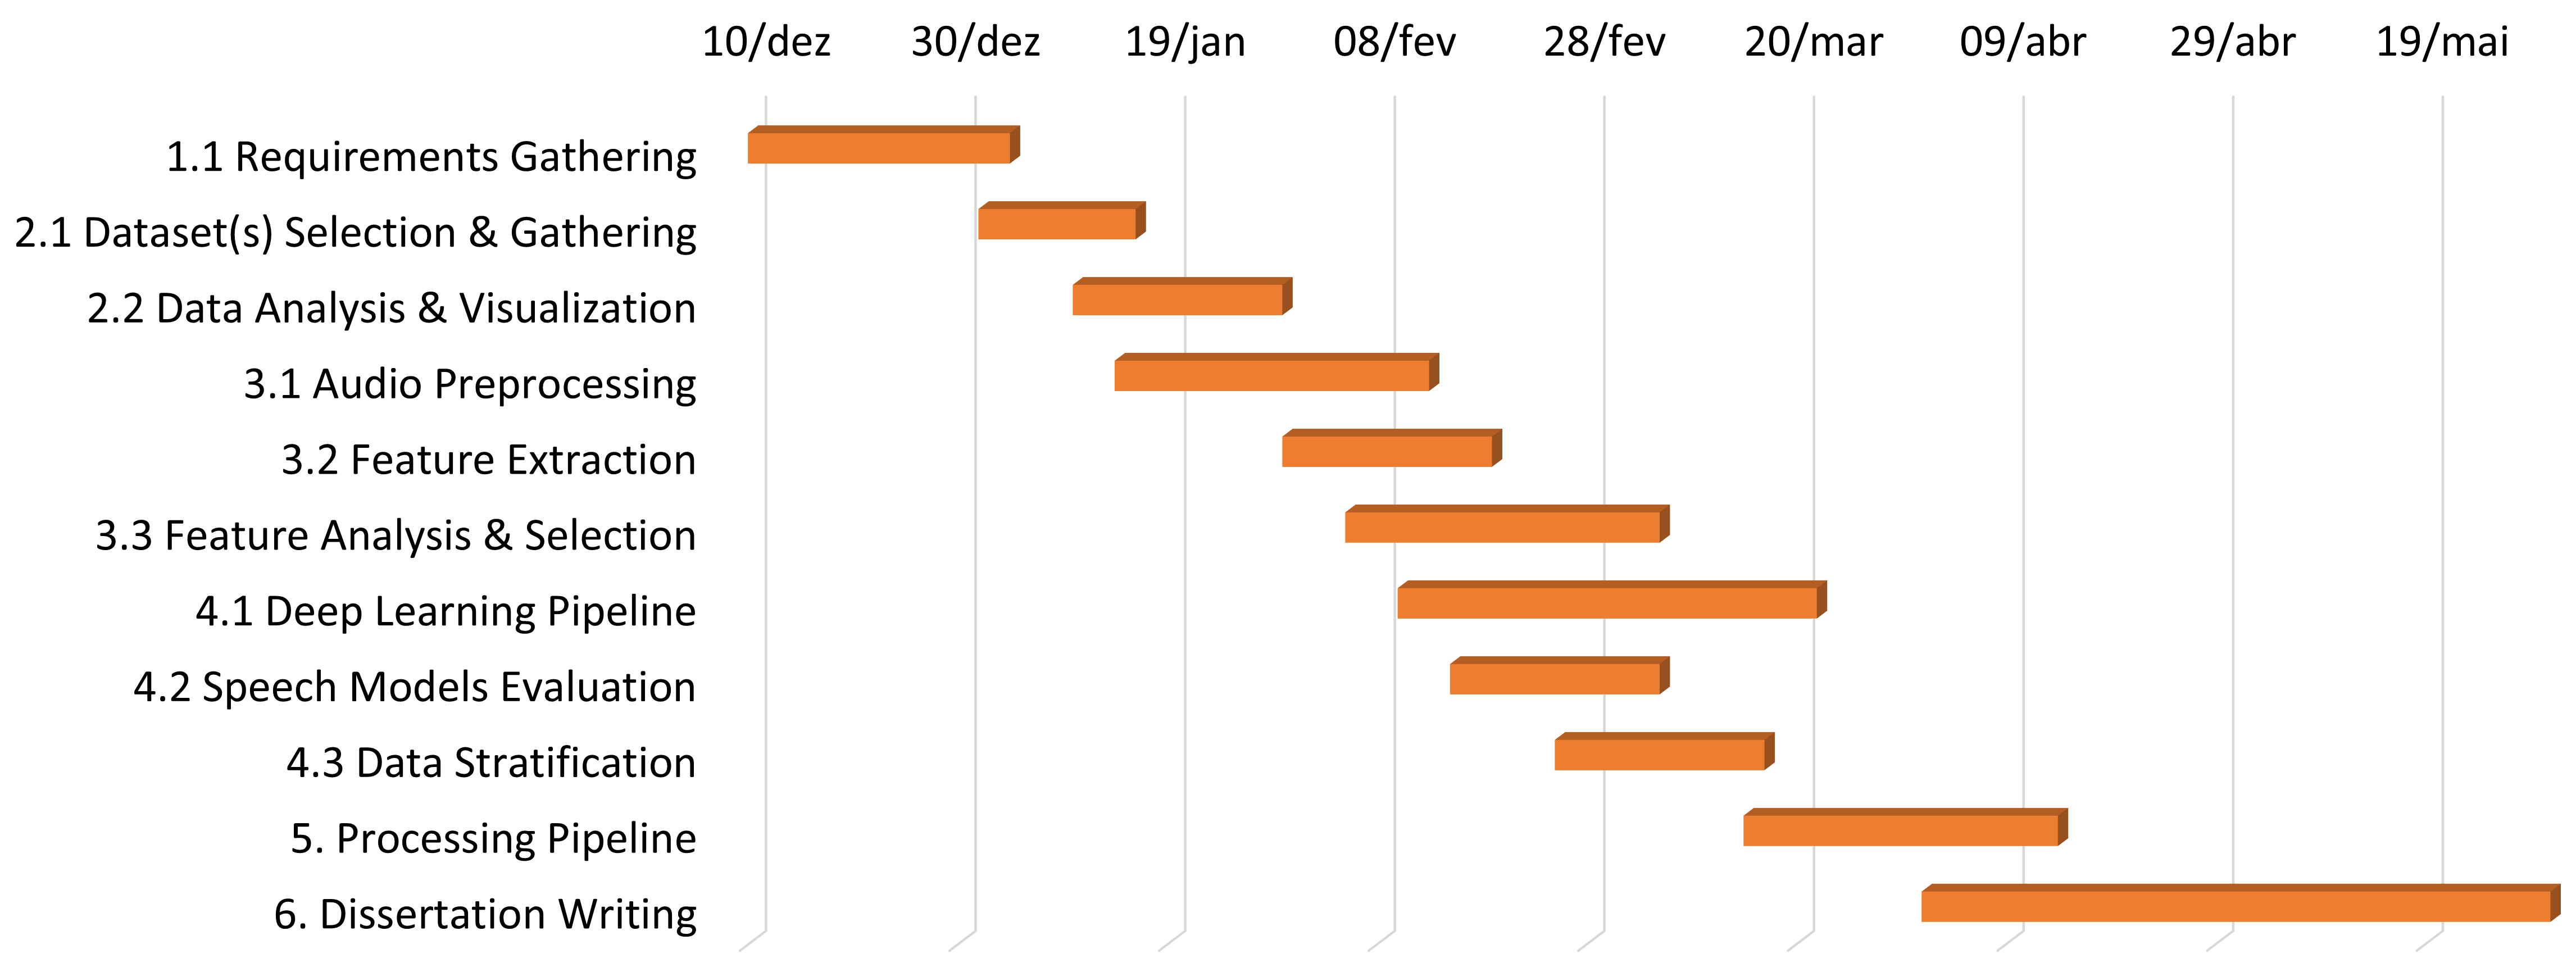
\includegraphics[width=\linewidth]{figs/3_methodology/gantt_chart.png}
	\caption{Gantt chart with the proposed work plan for this research.}
	\label{fig:gantt}
\end{figure}

\subsection{Requirements Gathering}

Initially, we conducted a requirements-gathering process to understand the needs, expectations, and constraints of our emotion recognition system. We identified specific use cases in which the system would be applied, and from there we were able to determine various requirements, including ethical considerations and technical requirements. These requirements served as the foundation for our defined objectives and strategies.


\subsection{Dataset}

\subsubsection{Dataset(s) Selection \& Gathering}

The next step is the selection of one or more audiovisual datasets that, in line with the \ac{sota} research, are preferably large and diverse (e.g., by featuring individuals of both genders, different scripts, contexts, etc.).

\subsubsection{Data Analysis \& Visualization}

Data analysis and visualization will allow us to explore, understand and display the data. Using various techniques such as statistical analysis, machine learning, and computational methods, we aim to extract information and then create graphical representations of it, in a way that allows us to better understand the dataset. 

\subsection{Audio Feature Engineering}

Once the dataset(s) have been selected, following the traditional feature-based approach, audio feature engineering will be required. In the context of machine learning, audio feature engineering involves preprocessing, extracting, and selecting relevant features from audio signals to build effective systems.

\subsubsection{Preprocessing}

\paragraph{Framing}

Speech framing, also called signal segmentation, is the process of dividing continuous speech signals into fixed-length segments. Speech typically stays consistent for a relatively short period, such as 20 to 30 ms. By dividing the speech signal into frames, local features can be extracted. Additionally, the relationship and information between the frames can be preserved by deliberately overlapping 30\% to 50\% of these segments. After creating the speech frames, researchers often apply a windowing function to smooth the edges and improve the time-frequency resolution of the signal \cite{Akay2020}.

\paragraph{Noise reduction}

Noise can have a significant negative impact on the quality of an audio signal by masking or distorting important features of the speech. It can also introduce variability into the audio data, making it harder for the machine learning model to generalize to new situations. The most successful methods for noise reduction are the Minimum Mean Square Error (MMSE) and Log-spectral Amplitude MMSE estimators \cite{Pohjalainen2016}.

\paragraph{Normalization}

Scale differences in features' values may affect the models' performance, especially those based on distance metrics to parameter estimation. So, it is advised to normalize features to prevent this effect. This can lead to more accurate and consistent results when applying the model to new data. The most widely used normalization techniques are z-normalization (also known as standardization) and min-max normalization \cite{Akay2020}.

\paragraph{\acl{vad*}}

\ac{vad*} is a technique used in speech processing to identify periods of speech in an audio signal. By focusing on analyzing the voiced speech and ignoring noisy or silent periods, \ac{vad*} can improve the accuracy of a system by reducing the influence of non-speech segments on the analysis. Furthermore, it can decrease the computational cost by reducing the amount of data to be processed. Commonly used methods for \ac{vad*} include zero crossing rate, short-time energy, and auto-correlation \cite{Akay2020}.

Figure \ref{fig:vad} demonstrates an instance where a \ac{vad*} system is applied to a speech signal, in this case, it is processing chunks with a duration of 1 second. It reduces the original signal of 10 seconds by half by identifying 5 voiced segments that are then fed to a \ac{ser} model \cite{Milling2022}.

\begin{figure}
	\centering
	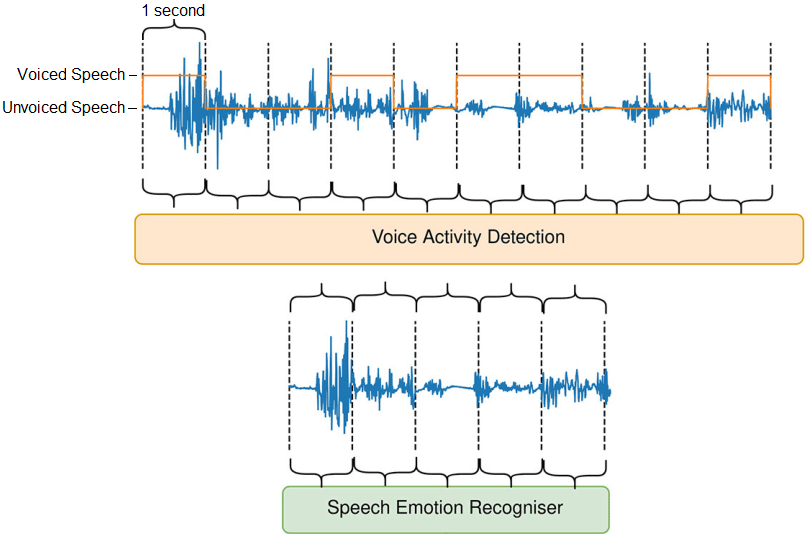
\includegraphics[width=.8\linewidth]{figs/3_methodology/speech_activity_detection.png}
	\caption{\acl{vad*} employment on an audio signal \cite{Milling2022}.}
	\label{fig:vad}
\end{figure}


\subsubsection{Feature Extraction}

Various techniques can be used to extract features from audio signals, such as time-domain analysis, frequency-domain analysis, and signal processing algorithms. These techniques can be used to extract features such as spectral features, temporal features, and statistical features. When studying the features extracted from speech audio signals, it is common to consider both global and local features \cite{PORIA201798}. Some emotions are more prominent at the beginning or end of a speech, so it is frequent to consider both global and local features to fully capture the temporal and emotional content of the signal.

\subsubsection{Feature Selection}

In order to achieve optimal performance, it is important to carefully select the features used in any model. Including redundant or uninformative features can degrade performance. By selecting and reducing the number of features, it is possible to maintain or even improve performance while using fewer resources and avoiding overfitting, also it becomes easier to understand the model's decision-making process and which features are most important.

\subsection{Models Implementation}

\subsubsection{Deep Learning Pipeline}

In addition, we will experiment and compare the effectiveness of automatic audio feature extraction-based approaches to \ac{ser}, using either the raw audio signals, \ac{mfccs}, or Mel spectrograms as input to deep learning models, some transfer learning techniques will also be explored.

\subsection{Speech Models Evaluation}

After we have chosen the relevant features through the feature selection process and completed the deep learning pipeline, we will test various models, and measure their performance by using appropriate metrics, to then identify the best classifiers for the traditional feature-based and \ac{dl}-based approaches.


\subsection{Data Stratification}

Data stratification refers to a process of dividing a dataset into subgroups, based on certain properties. We will test different ways of grouping the labeled data and interpreting their effects on the model's predictions, for example, by relabeling the angry and sadness samples as \textit{negative} samples. By doing this, we can discover potential biases in both the classifiers and the dataset(s), such as the individual's age, gender, and even the evaluation of the samples given by juries.


\subsection{Deployment}

\subsubsection{Processing Pipeline}

The most suitable model for offline and online scenarios will be analyzed and tested in a real-time scenario using an audio segmentation pipeline with \ac{vad*}.

\subsection{Dissertation Writing}

To conclude the work plan, we will focus on a comprehensive discussion of our research, including any potential challenges and limitations that we encountered and the steps we took to address them.

\section{Ethical Procedures and Concerns}

There are several ethical concerns when building emotion recognition systems, and in our case, we will address those related to \ac{ser} systems. One of them is that they may not be accurate in recognizing emotions for people with certain characteristics (age, gender, accents, speech disabilities, etc.), which is why we will address and quantify some potential biases in our models.

Another concern is that these systems may be used to monitor or control persons without their consent. Our models will only be in use on individuals that fully consented to submit their data for emotional evaluation purposes.

Additionally, there may be privacy concerns about personal data collected by these systems being vulnerable to hacks or used for unintended purposes. Our processing pipelines will only utilize the participant's streaming data for the \ac{ser} models input, and, will not store or use the sensitive data for any other purposes than the emotional analysis. We also decided to not use speech transcriptions, as it raises even greater privacy issues, due to capturing the actual words spoken and can reveal confidential data such as personal, financial, or business information.

In summary, we intend to be transparent about the system's capabilities and limitations and obtain informed consent before collecting and using any personal data.


\chapter{\ac{ser} Development}
\label{chapter:strat}

\section{Datasets}

In this section, we present a detailed account of the datasets employed in the development and evaluation of our \ac{ser} system.

The first dataset was utilized to investigate and select the most optimal features, evaluate the performance of classification models, and identify effective classification strategies.

\subsection{\ac{iemo}}

The \ac{iemo} database \cite{Busso2008}, created in \citeyear{Busso2008}, is an acted and elicited multimodal and multi-speaker database. It consists of 12 hours of audiovisual data, including video, speech, motion capture of face, and text transcriptions.

Sessions were manually segmented into utterances, spoken by 10 (5 female and 5 male) professional actors in fluent English. Each utterance was annotated by at least 3 human annotators in 9 categorical attributes, and, in addition, it was annotated with 3-dimensional attributes using the \ac{vad} emotion model. Similar to the development dataset, this data was collected using emotion elicitation techniques such as improvisations and scripts. Figure \ref{fig:bar_plots_distribution} from the research article \ref{Busso2008}, demonstrates that there is a similar amount of annotated labels on scripted and spontaneous sessions on this dataset.

\begin{figure}[H]
	\centering
	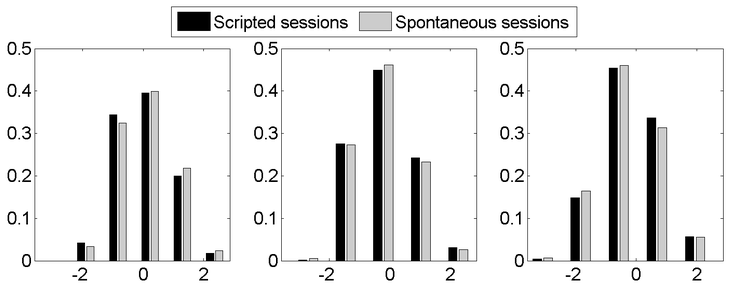
\includegraphics[width=.8\linewidth]{figs/4_1_traditional/scripted_spont_distribution.png}
	\caption{Distribution of the emotional content of the IEMOCAP corpus in terms of (a) valence, (b) activation, and (c) dominance. The results are separately displayed for scripted (black) and spontaneous (gray) sessions.}
	\label{fig:bar_plots_distribution}
\end{figure}


Overall, \ac{iemo} is a well-suited resource for our study, as the multimodal data, annotated using both discrete and dimensional models, allows us to perform a wide range of operations, researchers have also noted the high quality of this dataset, being frequently used in the literature for evaluating emotion recognition models. This enables us to make better comparisons of our own developed models, which is why we utilized it as a training and testing dataset for our \ac{ser} models and to explore strategies and biases by stratifying the data.

Most researchers when using this dataset perform 4 class emotion recognition, and also, consider the class \textit{excitement} as \textit{happiness}, due to their similarities and to even out the distribution of files per emotion. We decided to use the same data, as shown in the table \ref{tab:dataDist}, ending up with a total of 5531 audio files, each file recorded with a sample rate of 16000 Hertz.

\begin{table}[H]
	\centering
	\caption{Number of Audio Files Used per Emotion from the IEMOCAP dataset.}
	\label{tab:dataDist}
	\begin{tabular}{cc}
		\toprule
		Emotion & Number of Audio Files \\
		\midrule
		Anger 		&  1103\\
		Happiness 	&  1636\\
		Neutral	 	&  1708\\
		Sadness 	&  1084\\
		\bottomrule
	\end{tabular}
\end{table}


\subsection{Testing Datasets}

To evaluate the generalization ability of our final models trained on the IEMOCAP dataset, we tested them on three additional emotion datasets: eNTERFACE’05, CREMA-D, and EMO-DB. The inclusion of these datasets allows us to estimate the effectiveness and applicability of our proposed \ac{ser} system across diverse contexts.

\subsubsection{eNTERFACE'05}

The eNTERFACE’05 emotion database \cite{Martin2006} was designed and collected during the eNTERFACE’05 workshop in \citeyear{Martin2006}. The dataset contains audio and visual data from 42 subjects, coming from 14 different nationalities, as shown in Table \ref{tab:enterfaceDiversity}. Among the subjects, a percentage of 35 are men, while the remaining 7 are women, and, all the experiments were driven in English.

\begin{table}[H]
	\centering
	\caption{eNTERFACE'05 subjects nationalities}
	\label{tab:enterfaceDiversity}
	\begin{tabular}{lc|lc}
		\toprule
		Country &Number of Subjects &Country &Number of Subjects\\
		\midrule
		Belgium & 9 & Cuba     & 1\\
		Turkey  & 7 & Slovakia & 1\\
		France  & 7 & Brazil   & 1\\
		Spain   & 6 & U.S.A.   & 1\\
		Greece  & 4 & Croatia  & 1\\
		Italy   & 1 & Canada   & 1\\
		Austria & 1 & Russia   & 1\\
		\bottomrule
	\end{tabular}
\end{table}


This dataset contains discrete annotated emotions, where each subject was asked to listen to six successive short stories, each eliciting a particular emotion. If two human experts judged the reaction expressing the emotion unambiguously, then the sample was added to the database.  From the dataset files, we only used those annotated with emotions present in the \ac{iemo} and ended up with the files presented in Table \ref{tab:ent_files}. The diversity of accents present in the dataset and its authenticity, due to the data being elicited, make it a suitable choice for testing the models' performance in different contexts.

\begin{table}[H]
	\centering
	\label{tab:ent_files}
	\caption{Number of Audio Files Used per Emotion from the eNTERFACE'05 dataset.}
	\begin{tabular}{lr}
		\toprule
		Emotion     &   Number of Files \\
		\midrule
		Anger      	&               210 \\
		Happiness 	&               210 \\
		Sadness    	&               210 \\
		\bottomrule
	\end{tabular}
\end{table}


\subsubsection{EMO-DB}

The EMO-DB database is a German emotional database created by the Institute of Communication Science, Technical University, Berlin, Germany. Ten professional speakers (five males and five females) participated in the data recording.

Since this dataset contains German spoken utterances, it allows us to test more directly the models' limitations caused by the language bias present in training data.

\begin{table}[H]
	\centering
	\label{tab:emo_files}
	\caption{Number of Audio Files Used per Emotion from the EMO-DB dataset.}
	\begin{tabular}{lr}
		\toprule
		Emotion     &   Number of Files \\
		\midrule
		Anger   	&               127 \\
		Happiness   &                71 \\
		Neutral		&                79 \\
		Sadness     &                62 \\
		\bottomrule
	\end{tabular}
\end{table}


\subsubsection{CREMA-D}


The CREMA-D dataset includes clips from 91 actors spoken in English. These clips are from 48 male and 43 female actors between the ages of 20 and 74 coming from a variety of races and ethnicities (African American, Asian, Caucasian, Hispanic, and Unspecified).

This dataset provides a variety of data which is ideal to test a model's generalization ability across new datasets. The sentences were presented using one of six different emotions, but as mentioned before, we selected only the emotions present in the \ac{iemo}, resulting in 4898 audio files \ref{tab:crema_files}. 

\begin{table}[H]
	\centering
	\label{tab:crema_files}
	\caption{Number of Audio Files Used per Emotion from the CREMA-D dataset.}
	\begin{tabular}{lr}
		\toprule
		Emotion     &   Number of Files \\
		\midrule
		Anger   	&              1271 \\
		Happiness   &              1271 \\
		Neutral 	&              1087 \\
		Sadness     &              1269 \\
		\bottomrule
	\end{tabular}
\end{table}



\section{Audio Preprocessing}

To prepare the collected audio data for use in machine learning models, audio preprocessing techniques are required. In this section, we will explore important aspects of audio preprocessing: noise reduction, feature extraction, analysis, and selection.

\subsection{Noise Reduction}

Spectral Gating: Common strategy for denoising music by gating the signal only on high level sounds.

Noisereduce is a noise reduction algorithm in python that reduces noise in time-domain signals like speech, bioacoustics, and physiological signals. It relies on a method called "spectral gating" which is a form of Noise Gate. It works by computing a spectrogram of a signal (and optionally a noise signal) and estimating a noise threshold (or gate) for each frequency band of that signal/noise. That threshold is used to compute a mask, which gates noise below the frequency-varying threshold.

Non-stationary Noise Reduction
The non-stationary noise reduction algorithm is an extension of the stationary noise reduction algorithm, but allowing the noise gate to change over time.
When you know the timescale that your signal occurs on (e.g. a bird call can be a few hundred milliseconds), you can set your noise threshold based on the assumption that events occuring on longer timescales are noise.
This algorithm was motivated by a recent method in bioacoustics called Per-Channel Energy Normalization.
Steps of the Non-stationary Noise Reduction algorithm
A spectrogram is calculated over the signal
A time-smoothed version of the spectrogram is computed using an IIR filter aplied forward and backward on each frequency channel.
A mask is computed based on that time-smoothed spectrogram
The mask is smoothed with a filter over frequency and time
The mask is appled to the spectrogram of the signal, and is inverted

$nr_x = nr.reduce_noise(y=x, sr=sr, n_fft=2048, hop_length=512, prop_decrease=.75, time_constant_s=1)$


\subsection{Audio Trim}

3. Trim silence in the beginning and end.
30 decibels and lower are considered as silence


% !TeX spellcheck = en_US
\section{Traditional Feature-Based \ac{ser}}


\subsection{Feature Extraction}

The first step in a traditional approach is feature extraction to transform raw audio data into a set of informative features that can capture key characteristics of the signal.

In this regard, the widely-used Librosa toolkit was employed to extract various audio features, from the audio files of the \ac{iemo} dataset, and subsequently, they were processed using statistical metrics. The extracted features and associated metrics are summarized in Table \ref{table:extractedFeat}, with a total of 327 extracted features.

\begin{table}[h]
	\centering
	\caption{Extracted audio features and the statistical functions applied.}
	\label{table:extractedFeat}
	
	\begin{tabular}{@{}cc@{}}
		\toprule
		Audio Features & Statistical Functions \\
		\midrule
		&  \multirow{10}{*}{\begin{tabular}{@{}c@{}}Minimum\\Mean\\Maximum\\Median\\25th percentile\\75th percentile\\Spikes\footnotemark[1]\\Variance \\Standard Deviation\\Sum\\Kurtosis\footnotemark[2]\\Skew\footnotemark[2]\end{tabular}} \\
		\acp{mfccs} 1 - 21 & \\
		Mel Spectrogram & \\
		Root-Mean-Square & \\
		Chromagram & \\
		Spectral Centroid & \\
		Spectral Contrast & \\
		Spectral Bandwith & \\
		Roll-Off Frequency & \\
		Tonnetz & \\
		Zero-Crossing Rate & \\
		& \\
		\bottomrule
		\multicolumn{2}{l}{\footnotemark[1]\footnotesize{Custom function detailed on the feature selection subsection \ref{spikes:metric}.}} \\
		\multicolumn{2}{l}{\footnotemark[2]\footnotesize{Only for the \acp{mfccs}.}} \\
	\end{tabular}
\end{table}

\subsection{Feature Analysis}

An important task following feature extraction is analyzing and interpreting the extracted data to gain a deeper understanding of the audio signals and the features that describe them.

\subsubsection{Audio Features Visualization}

In this process, we visually analyzed and interpreted the features' data by graphically representing each feature from an audio segment. The figures in Section \ref{app:1} of the appendix demonstrate some of the graphics we used to visualize the features.

\subsubsection{Spikes Metric}
\label{spikes:metric}

Initially, wave plots were observed, and we noted consistency in the number of high values. For this reason, we created a custom metric that calculates those high values, which we called "spikes", from the features' data.

In Figure \ref{fig:zcrSpikes}, it is possible to visualize the zero crossing rates' wave plots in different emotions. The horizontal line represents the threshold that we considered, any value above was considered to be a spike, which is annotated with red dots in the graphic. The threshold used was manually tested and obtained decent consistency of the number of spikes, within an emotion, by using the mean value of the feature plus 2\% of the standard deviation. To account for different-length audio signals, it was also divided the number of spikes to the total length of the data, as the Code Snippet \ref{spikes:code} demonstrates. Consequently, this metric was also tested and applied to every other audio feature.

\begin{figure}[H]
	\centering
	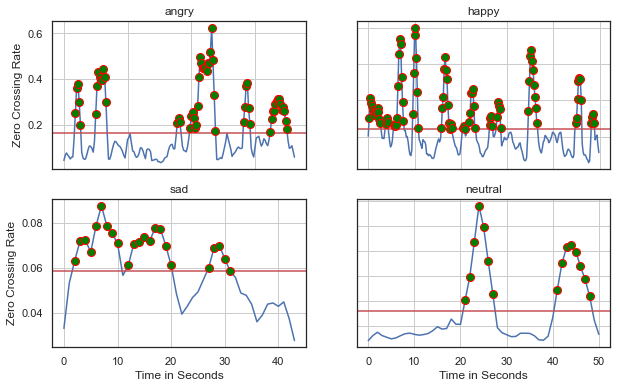
\includegraphics[width=.7\textwidth]{figs/4_1_traditional/zcr_waveplot_spikes.png}
	\caption{Zero crossing rate wave plot annotated with spikes.}
	\label{fig:zcrSpikes}
\end{figure}

\begin{listing}[H]
	\begin{minted}{python}
def spikes(data):
	mean = np.mean(data)
	std = np.std(data)
	threshold = mean + np.abs(std) * 2 / 100
	num_spikes = 0
	for value in data:
		if value >= threshold:
			num_spikes += 1
	return num_spikes / len(data)
	\end{minted}
	\caption{Python code for calculating the spikes metric.}
	\label{spikes:code}
\end{listing}



\subsubsection{Bar Plots}

Furthermore, bar plots were useful for viewing the overall extracted features' data plainly and quickly, and to understand the numeric values of each feature and metric used on it.

For example, figure \ref{fig:melBarPlot} shows clear differences in the mean values for some metrics used on the Mel Spectrogram. Other bar plots are presented in the appendix \ref{app:2}.

\begin{figure}[H]
	\centering
	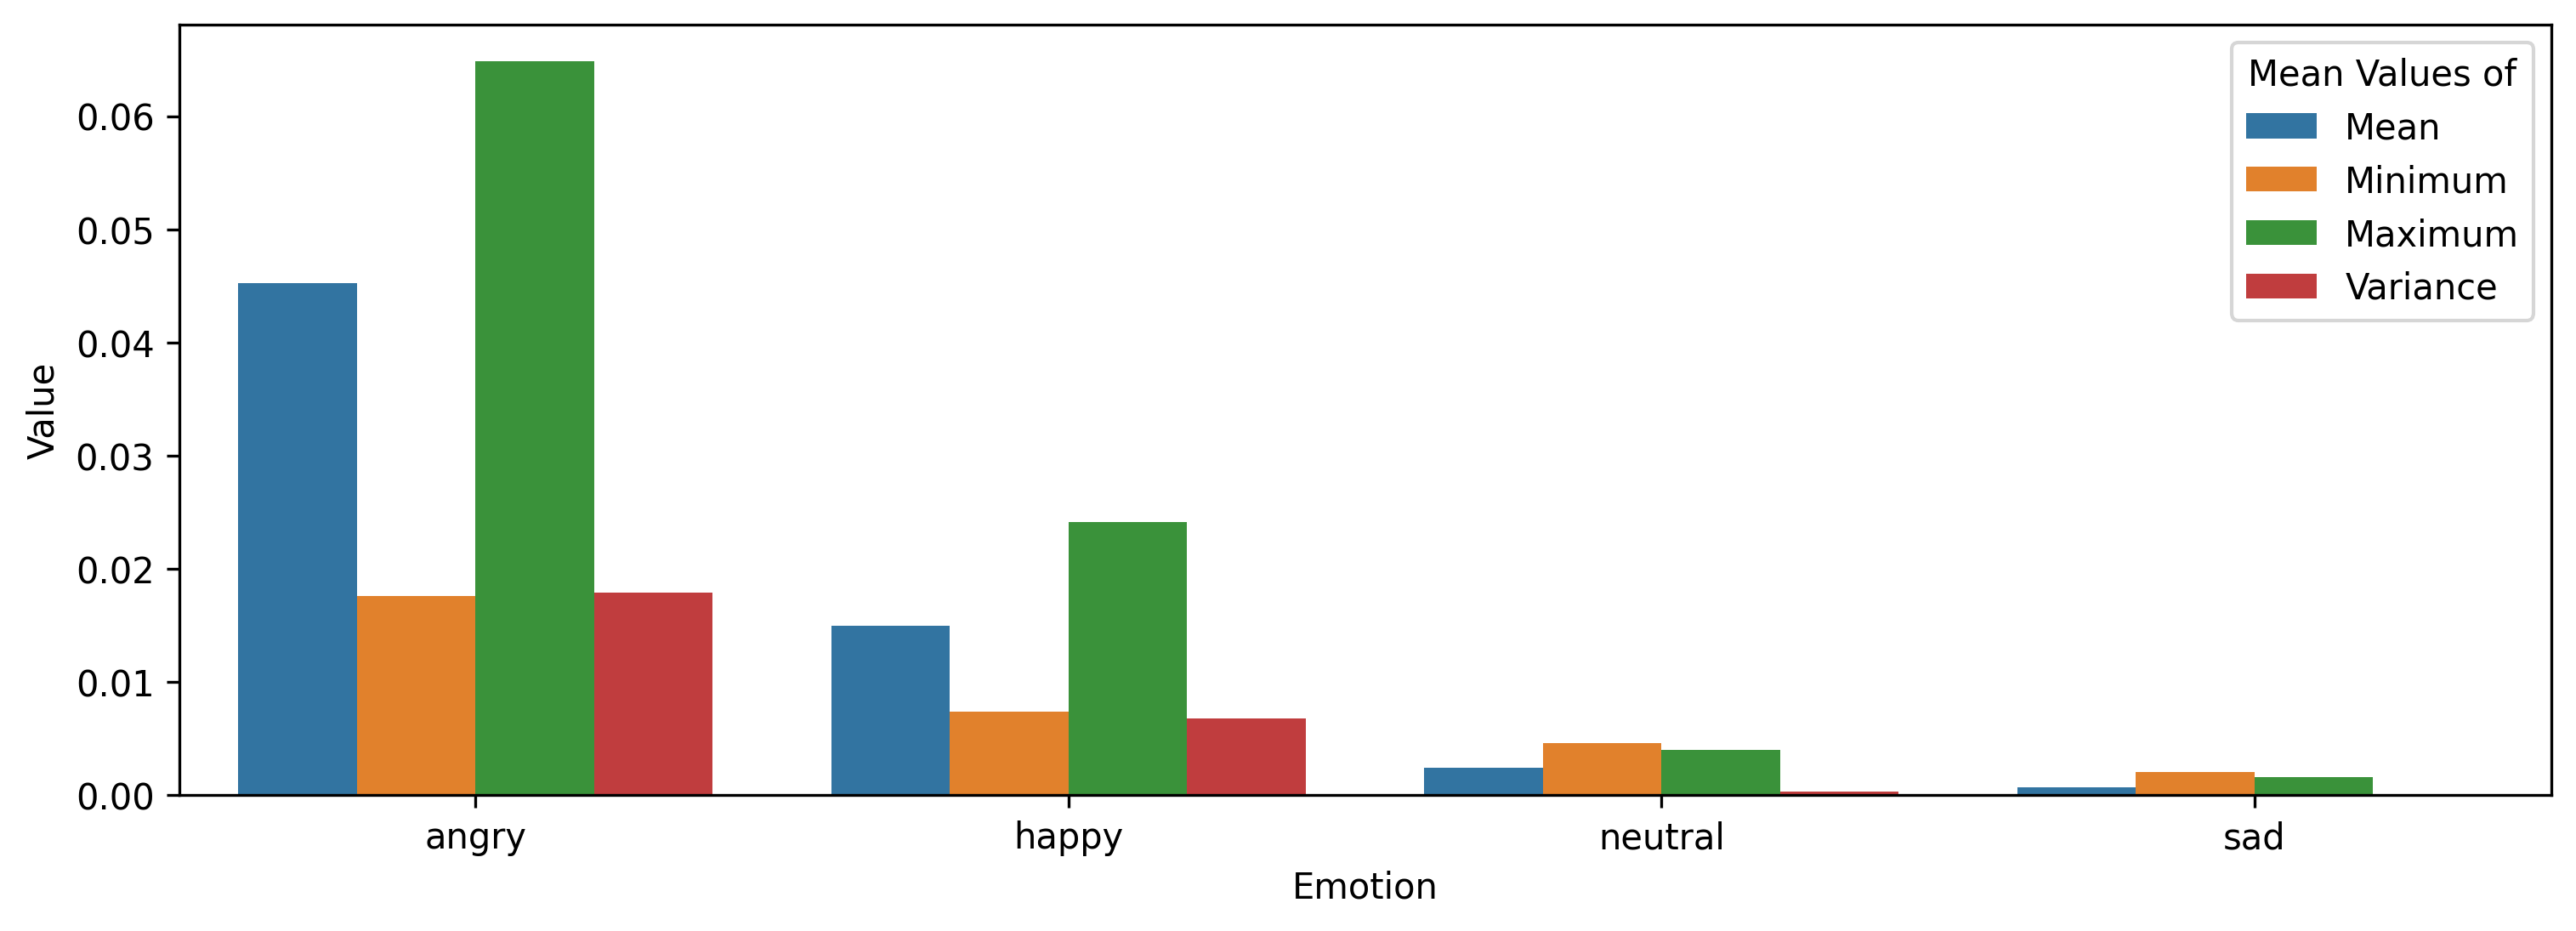
\includegraphics[width=\textwidth]{figs/4_1_traditional/meanFeatBarPlot.png}
	\caption{Bar plots mean for metrics used on the mel spectrogram feature.}
	\label{fig:melBarPlot}
\end{figure}


\subsubsection{Wave Plots with Surrounding Areas}

During the feature study process, it was observed the wave plots of some features surrounded by a small area above and below the original wave (defined through a selected threshold). This was done to corroborate how well the feature describes different emotions. A high degree of overlap between surrounding areas of a feature, for a given emotion, could indicate that the feature  has consistent values and is relevant for identifying that emotion.

Figure \ref{fig:zcrAreaOnly1} is an excerpt of the figure \ref{fig:zcrArea} in the appendix \ref{app:3}, and it demonstrates an example of this analysis for the zero crossing rate with 5 different subjects on the same sentence for the anger emotion. From this graphic, it was observed that there is an overlap between the surrounding areas for each emotion, which allows us to conclude that the feature has utility for describing each emotion. However, due to the different lengths of each audio segment, it is ambitious to guarantee this conclusion.

\begin{figure}[H]
	\centering
	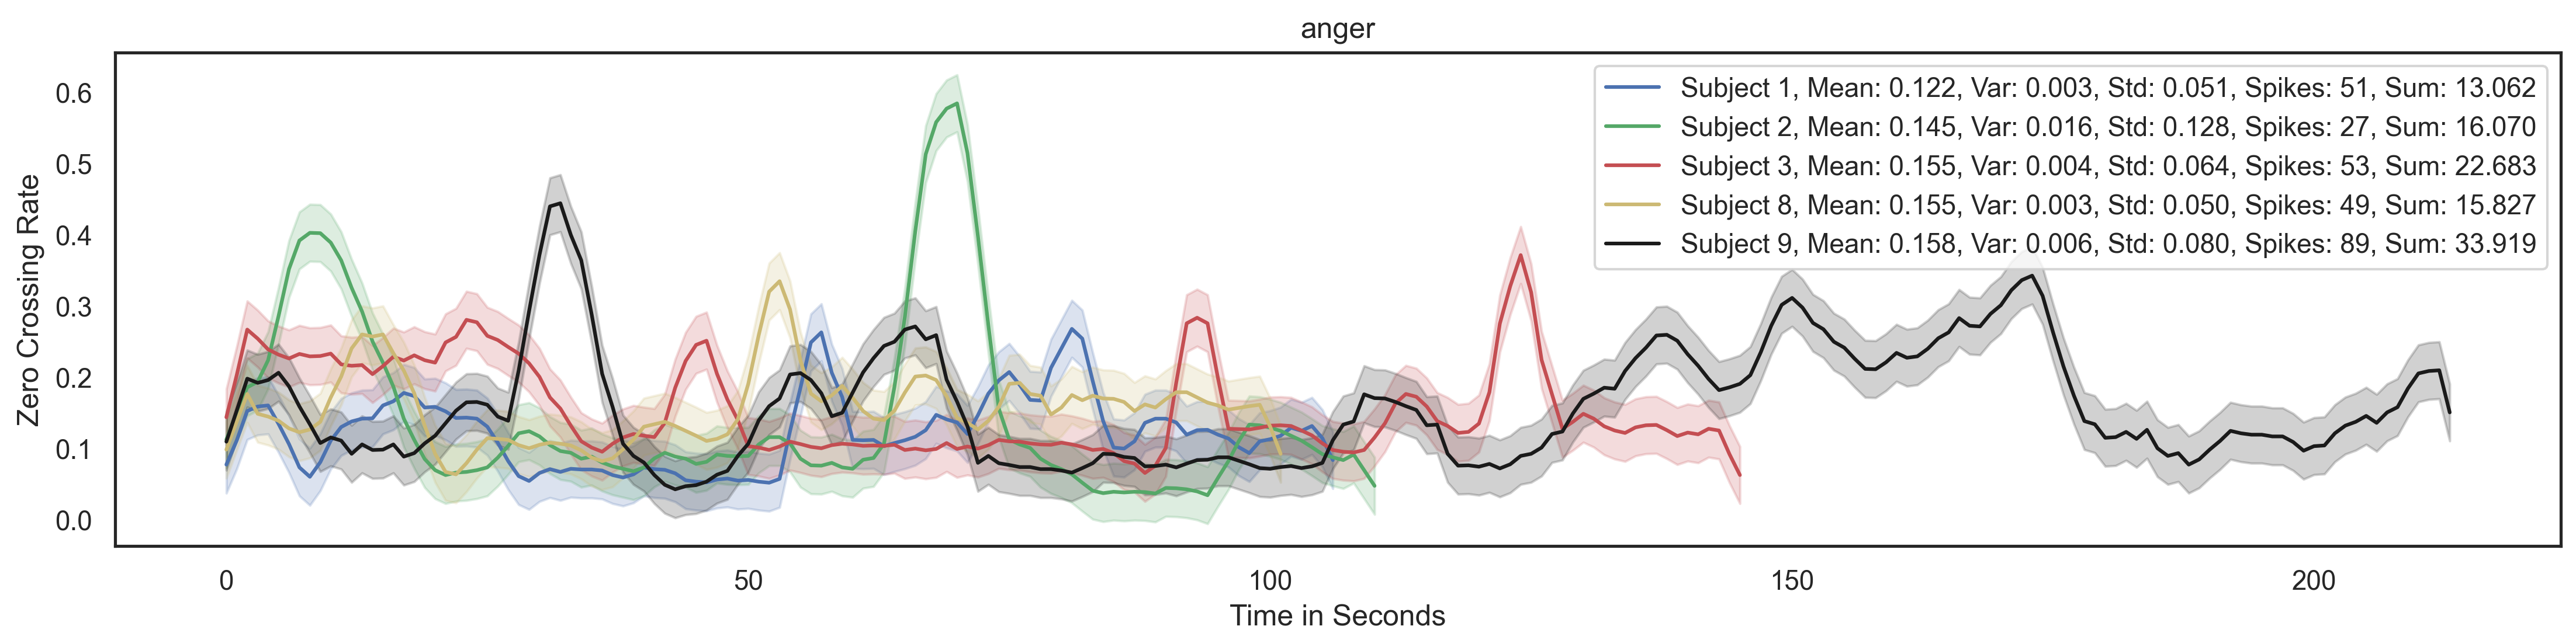
\includegraphics[width=1\linewidth]{figs/4_1_traditional/zcrAreaOnly1.png}
	\caption{Zero crossing rate wave plot with a surrounding area of five male subjects for the same utterance with the anger emotion.}
	\label{fig:zcrAreaOnly1}
\end{figure}

This same idea can also be used to determine whether a feature is favorable for creating a distinction between different emotions, which is naturally useful for the problem of classifying emotions. The conclusion can be drawn by observing the opposite of the previous case. If the areas around the feature, on different emotions, do not heavily overlap, it may be an indicator that the feature can be able to discriminate emotions. Figure \ref{fig:zcrAreaSameSubj} displays six zero crossing rates of one subject saying the same sentence but expressing different emotions. As previously mentioned, since audio lengths are different, it is challenging to draw a direct and well-founded conclusion.

\begin{figure}[H]
	\centering
	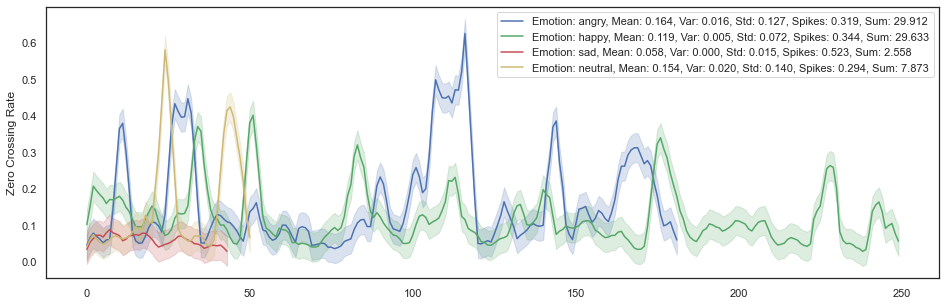
\includegraphics[width=.8\linewidth]{figs/4_1_traditional/zcr_male_same_subject.png}
	\caption{Zero crossing rate wave plots with a surrounding area of a single male subject and sentence for all different emotions.}
	\label{fig:zcrAreaSameSubj}
\end{figure}

Overall, this approach of surrounding wave plots with areas provided us valuable insight into the ability of a feature to describe and distinguish emotions, though it is limited by the varying lengths of audio segments.

\subsubsection{Variation Plots}

Another graph made was a variation plot, to perceive the differences in the features' values, across several audios for the same emotion. Figure \ref{fig:zcrMeanVar} shows an example of this type of plot for the mean zero crossing rate value across 50 speech utterances for all emotions. Other examples of this type of graphic are also in the appendix \ref{app:4}.

\begin{figure}[H]
	\centering
	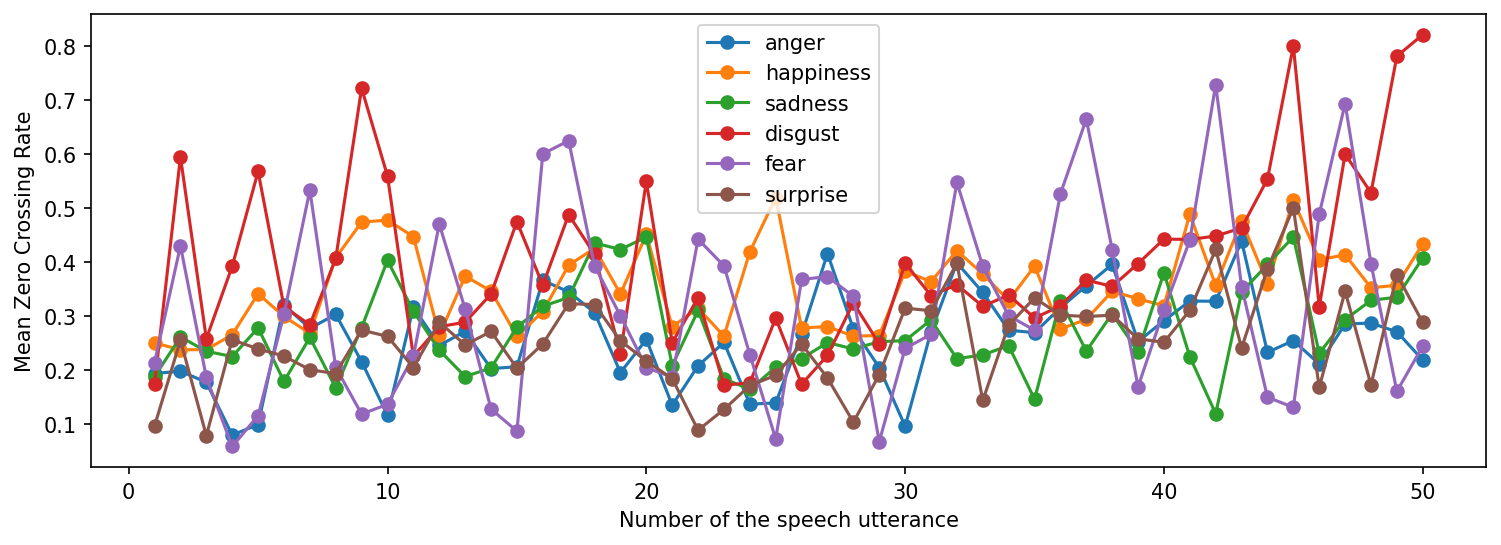
\includegraphics[width=\linewidth]{figs/4_1_traditional/meanZCRVar.png}
	\caption{Zero crossing rate mean values variation plot along 50 audios of speech utterances for all emotions.}
	\label{fig:zcrMeanVar}
\end{figure}

A common observation for most extracted feature plots was that the values were not consistent across multiple audio segments for the same emotion. However, the number of audio segments used in this study was relatively low (only 50) to observe big variability changes, but increasing the number of audio segments would also make it more challenging to observe such variability through a simple visual inspection.

\subsubsection{Box Plots}

Finally, we employed box plots to visualize the distribution of the features on different subjects, as well as to compare the values for each emotion. An example of this type of plot is shown in Figure \ref{fig:zcrMeanBoxPlot}, which displays the mean zero crossing rate feature for all emotions and different subjects. 

\begin{figure}[H]
	\centering
	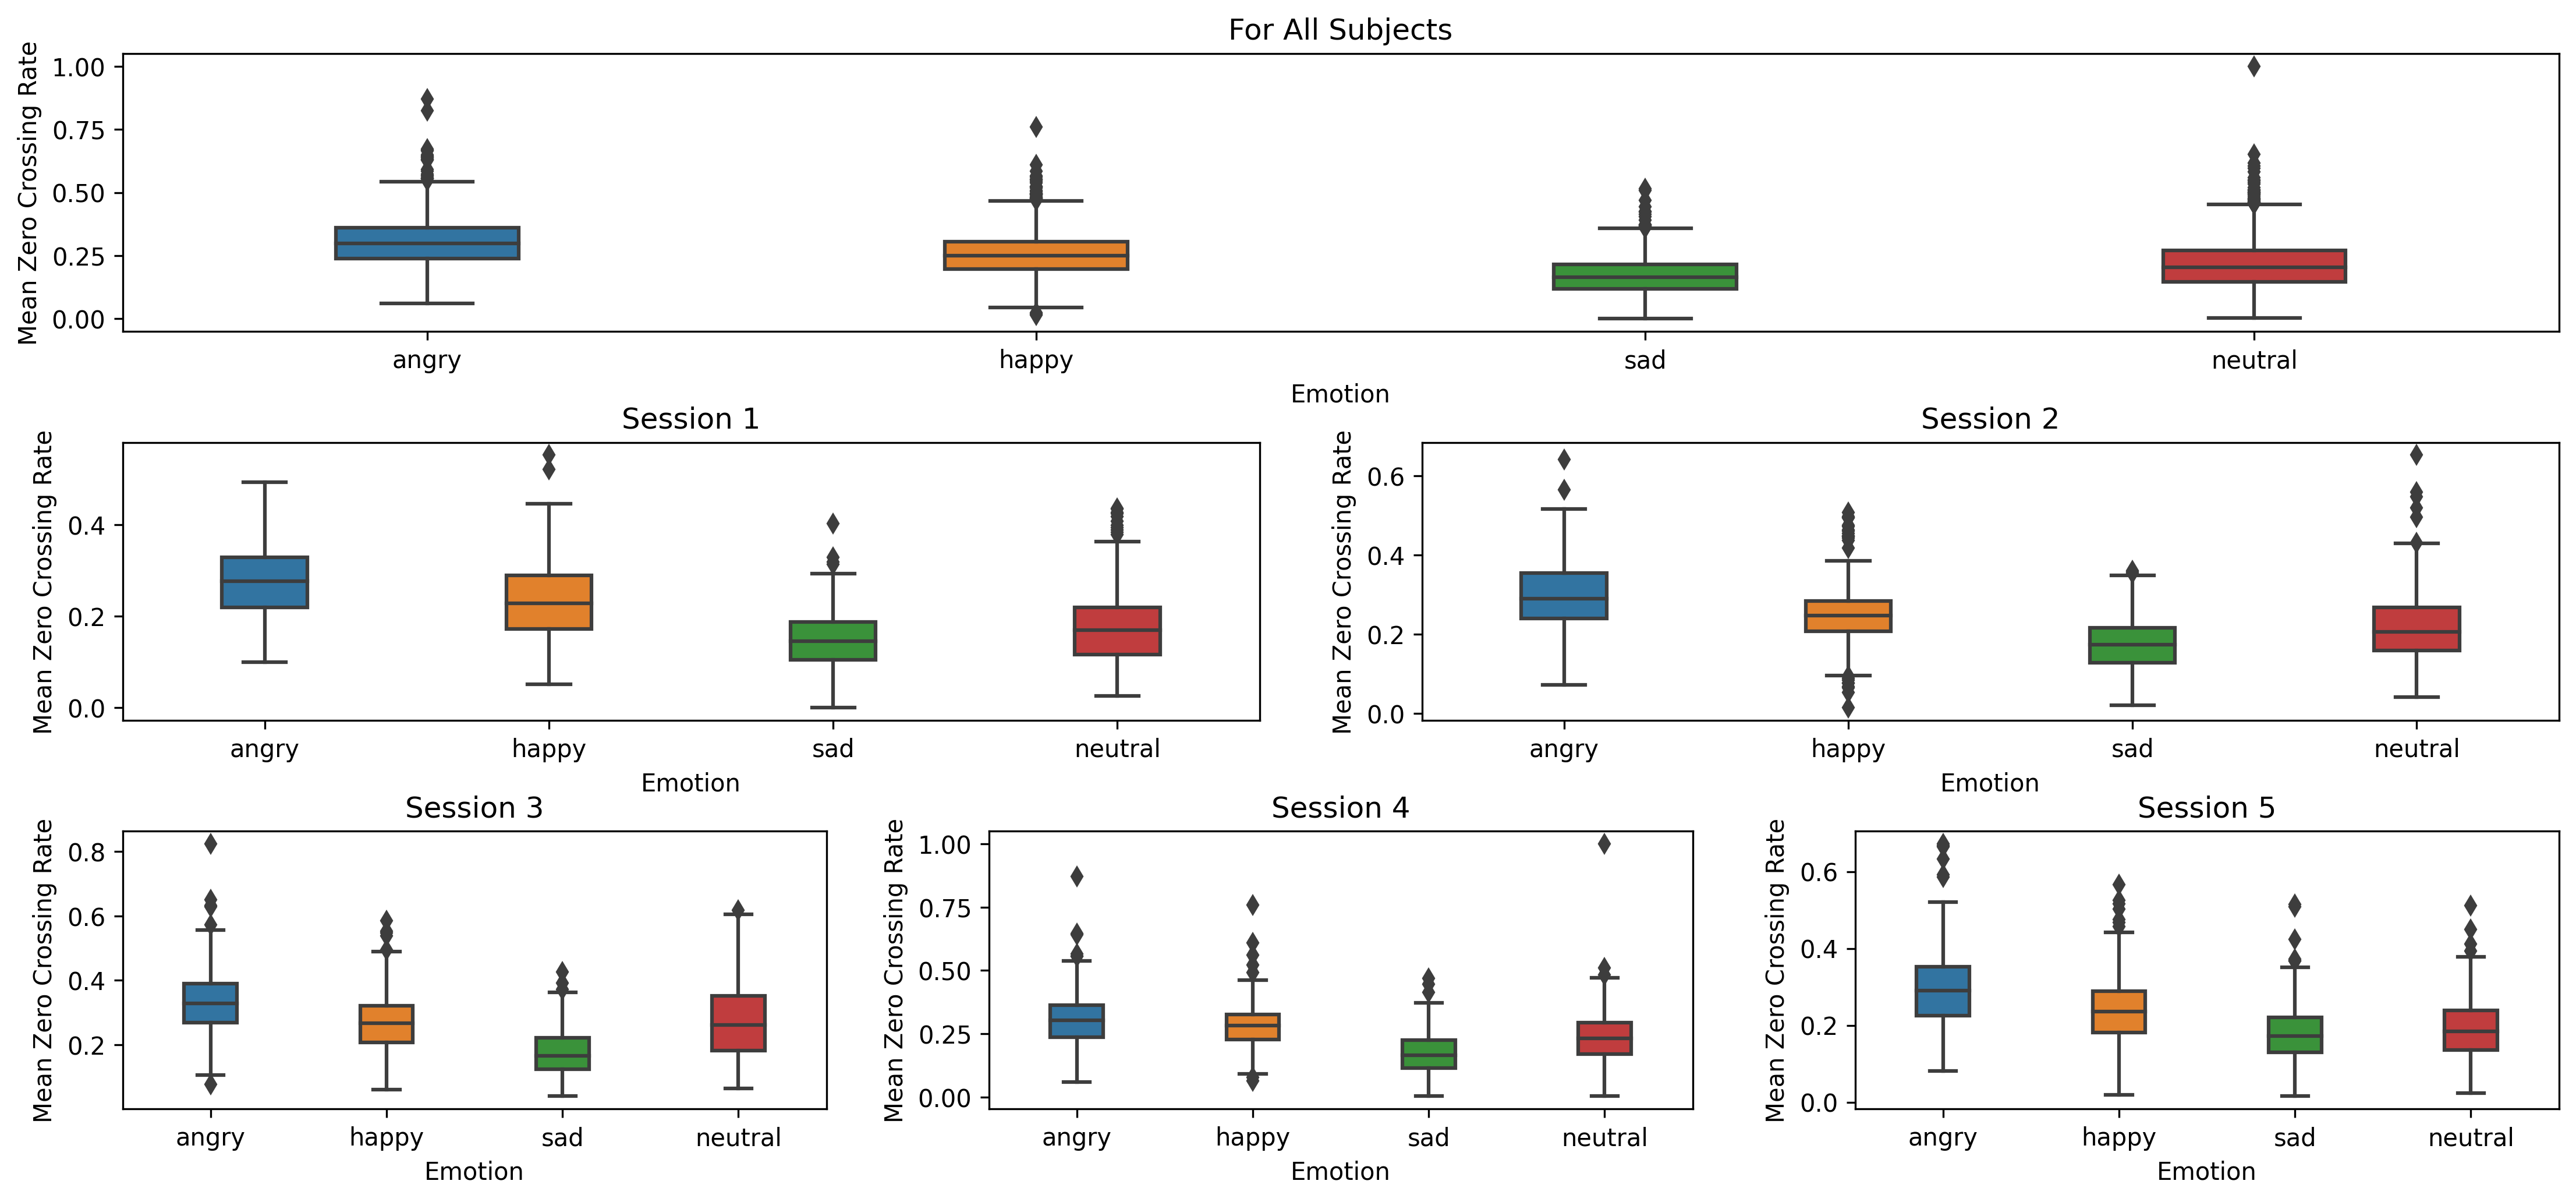
\includegraphics[width=\linewidth]{figs/4_1_traditional/mean_zcr_box_plot.png}
	\caption{Zero crossing rate mean values box plot for all emotions and different subjects.}
	\label{fig:zcrMeanBoxPlot}
\end{figure}

The primary purpose of using these plots was to provide a simple and intuitive representation of each feature. By comparing the values across all subjects or a selected few, any noticeable differences in feature values for each emotion could be easily perceived.

\subsection{Feature Selection}

After the process of feature analysis, the next step in \ac{ser} development is feature selection. Feature selection is a technique to choose a subset of the original set of features that are most relevant for the given task. The process of feature selection is aimed to improve the accuracy of the model and reducing the problem's complexity by removing redundant or irrelevant features. 

The objective is to choose a smaller set of features that retain enough information for good classification performance while being computationally efficient. Hence, a smaller subset of features that can provide effective classification results is preferred over the larger set of features that may be computationally expensive and redundant.

\subsubsection{\acl{cfs}}

Correlation among our extracted features is common since many of them use the same audio descriptor but with a different metric applied to them. Therefore, a correlation matrix for all 327 extracted features was calculated using the Pearson method, presented in figure \ref{fig:allAudioFeat}.

A \ac{cfs} was performed by selecting every pair of features with a Pearson correlation coefficient absolute value of 0.6 or above, then it was removed the feature with the highest average correlation value with all the other features. This process resulted in the elimination of 229 features, leaving 98 features for subsequent analysis. The correlation matrix after the feature selection process is presented in figure \ref{fig:highAudioFeat}.

\begin{figure}[H]
	\begin{subfigure}{.5\textwidth}
		\centering
		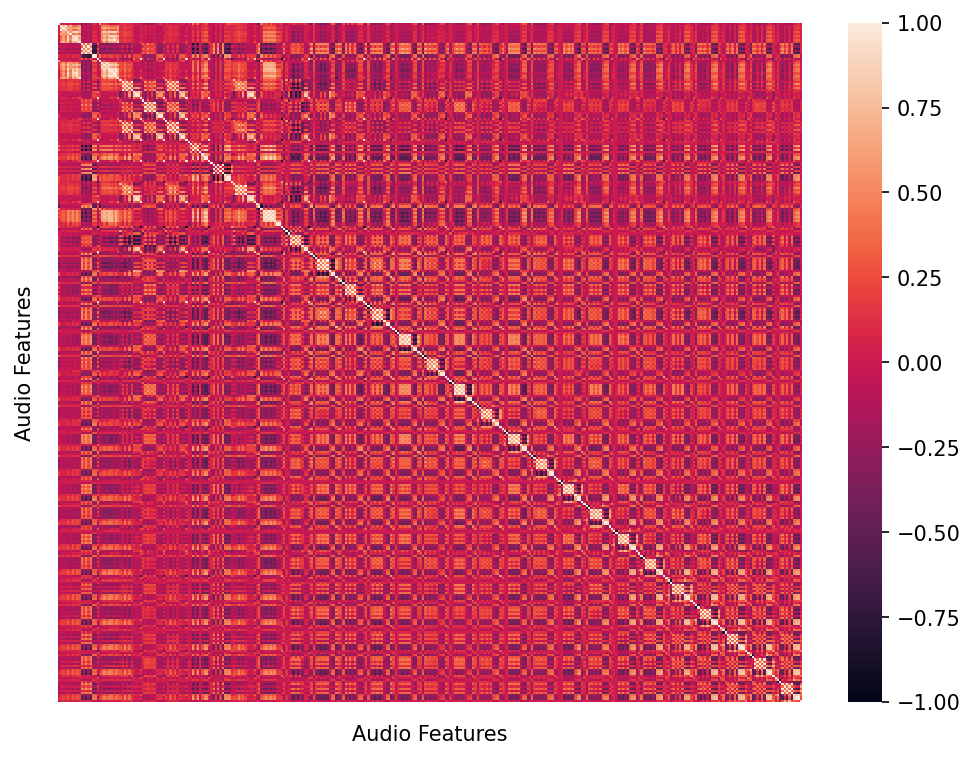
\includegraphics[width=\linewidth]{figs/4_1_traditional/allCorrMatrix.png}
		\caption{Correlation matrix of all the features.}
		\label{fig:allAudioFeat}
	\end{subfigure}%
	\begin{subfigure}{.5\textwidth}
		\centering
		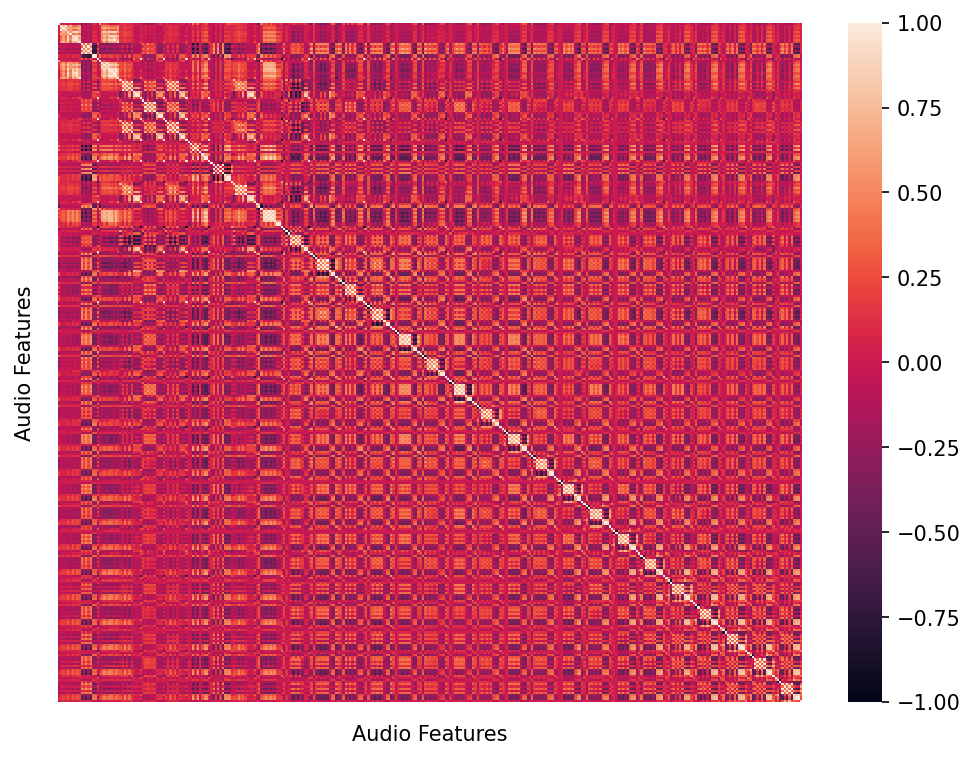
\includegraphics[width=\linewidth]{figs/4_1_traditional/highCorrMatrix.png}
		\caption{Correlation matrix after \ac{cfs}.}
		\label{fig:highAudioFeat}
	\end{subfigure}
	\caption{Audio features' correlation matrices before and after \ac{cfs}.}
\end{figure}

\subsubsection{Selecting an Initial Classifier}

Along this process, it became necessary to choose a model to be used in computationally expensive feature selection methods. Consequently, several estimators were tested for their performance in classifying emotions.

To this end, we conducted 5-fold \ac{cv} and compared the mean and standard deviation accuracies of all folds, as well as the total execution time for various classifiers using default parameters from the scikit-learn library \cite{pedregosa2011scikit}. The input given to the models is the set of features obtained after \ac{cfs}, as shown in Table \ref{tab:modelsPerformance}.

\begin{table}[H]
	\caption{Performance of various classifiers in 5-fold \ac{cv} using the features obtained after \ac{cfs}.}
	\centering
	\label{tab:modelsPerformance}
	\begin{tabular}{lrrr}
		\toprule
		Classifiers &  Accuracy & Training Time (s) \\
		\midrule
		\ac{xgb}                &        0.617$\pm$0.013  & 17.628 \\
		\ac{rf}                &        0.578$\pm$0.010  &  7.451 \\
		Ridge                  &        0.565$\pm$0.014  &  0.078 \\
		Extra Trees            &        0.561$\pm$0.005  &  1.831  \\
		AdaBoost               &        0.520$\pm$0.008  & 12.205  \\
		C-Support Vector       &        0.504$\pm$0.018  &  5.081 \\
		DecisionTree           &        0.450$\pm$0.022  &  1.886 \\
		Multi-layer Perceptron &        0.446$\pm$0.027  &  4.821 \\
		\bottomrule
	\end{tabular}
\end{table}

Based on the evaluation results, the \ac{rf} classifier was chosen for further analysis. This model exhibited the second-best average accuracy across the 5 folds, however, it was much faster than the \ac{xgb} to train. Therefore, \ac{rf} was the selected model for performing computationally expensive feature selection methods.


\subsubsection{Backwards Selection}

In the pursuit of completing the feature selection process, a sequential feature selection with backward propagation was employed. This method involves performing a 5-fold \ac{cv} with the previously selected \ac{rf} classifier, using all features except one, and then removing one feature based on the lowest mean accuracy of the 5 folds. This iterative process continues until only one feature remains.

A method was then developed to select the furthest and highest accuracy. This method resembles the standard maximum, but it multiplies the maximum value by a threshold value of $0.99$ so that it can find close to the maximum values that have more features removed, creating a balance between accuracy and the number of features. Figure \ref{fig:backProp1} displays the mean accuracies obtained at each step and the chosen furthest highest accuracy.

\begin{figure}[H]
	\centering
	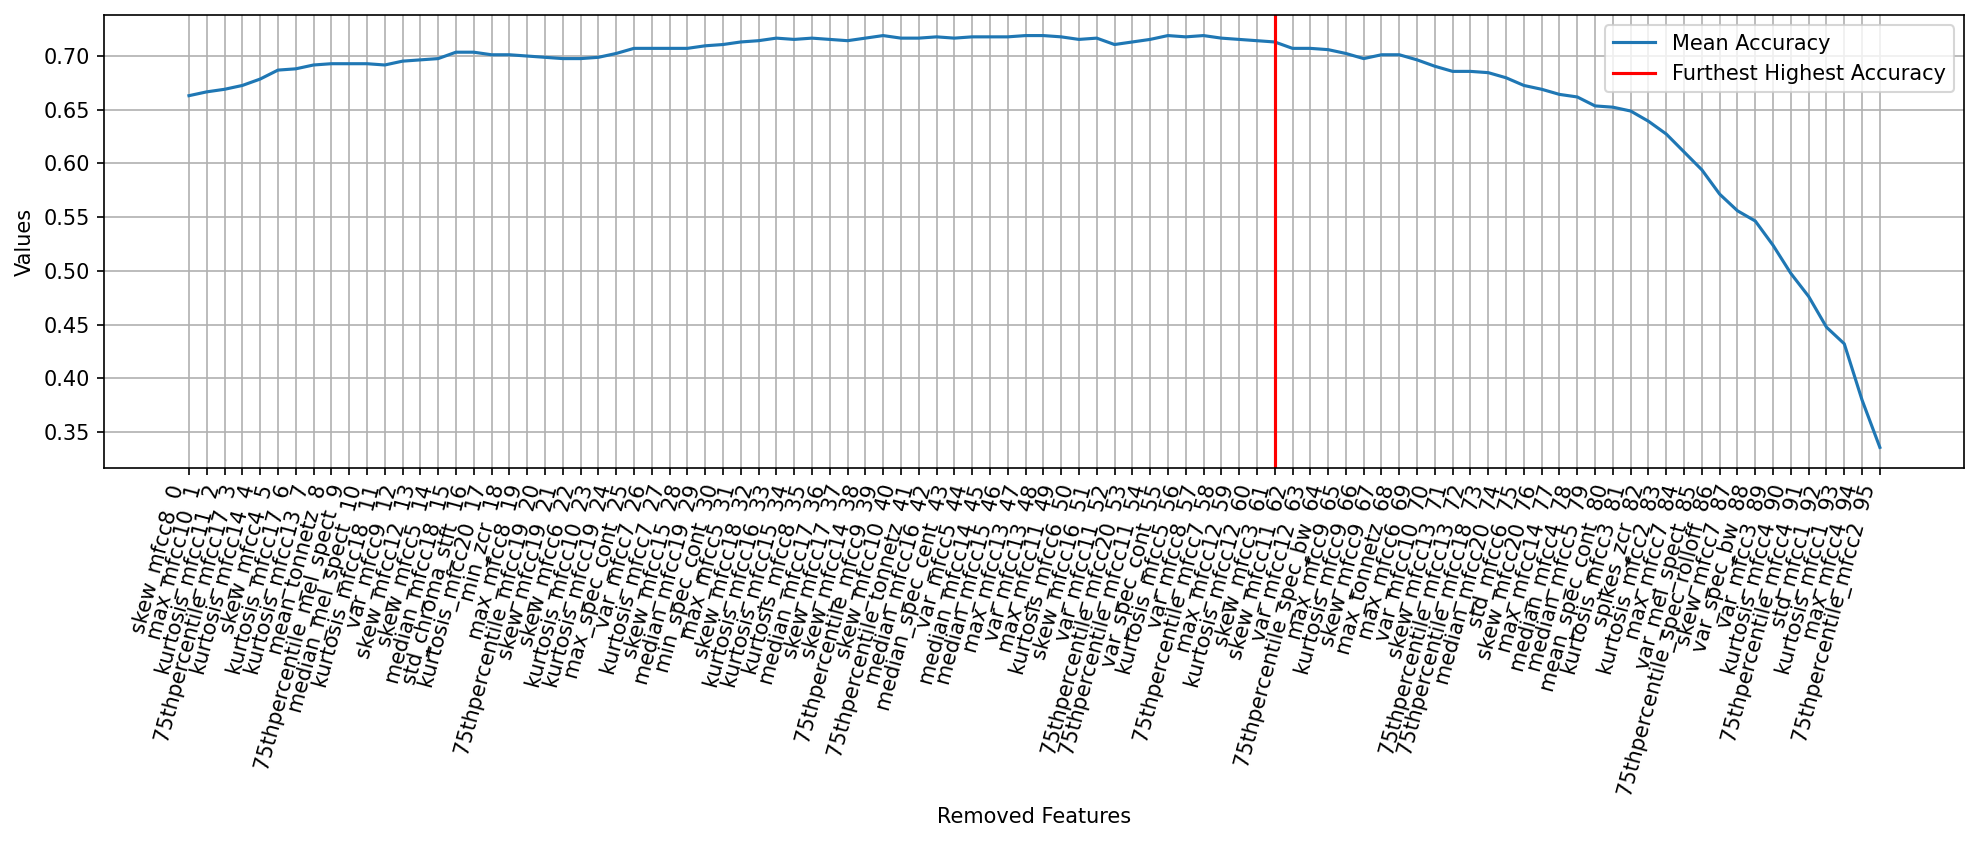
\includegraphics[width=1\linewidth]{figs/4_1_traditional/backProp1.png}
	\caption{Sequential feature selection with backward propagation using the mean accuracy as the selection criteria.}
	\label{fig:backProp1}
\end{figure}

This process led to the elimination of 65 features from the initial set of 98 obtained after \ac{cfs}, leaving a total of 33 features, as shown in Table \ref{tab:selectedFeat}.

\begin{table}[H]
	\caption{Final set of the 33 selected features.}
	\centering
	\label{tab:selectedFeat}
	\resizebox{\textwidth}{!}{%
		\begin{tabular}{ll}
			\toprule
			Metric & Audio Features \\
			\midrule
			Spikes & Mel-Spectrogram, Chromagram, Zero Crossing Rate, MFCC-6, MFCC-16, MFCC-19 \\
			Mean & Spectral Bandwidth, MFCC-13, MFCC-15, MFCC-17, MFCC-19, MFCC-20 \\
			Maximum & Spectral Bandwidth, MFCC-5, MFCC-7, MFCC-10, MFCC-11 \\
			Variance & Mel-Spectrogram, MFCC-1, MFCC-3, MFCC-5, MFCC-8 \\
			Kurtosis & MFCC-12, MFCC-17, MFCC-18 \\
			25th Percentile & Chromagram, Root Mean Square \\
			75th Percentile & MFCC-7, MFCC-11 \\
			Sum & MFCC-10, MFCC-12 \\
			Median & MFCC-5 \\
			Min & Zero Crossing Rate \\
			\bottomrule
		\end{tabular}
	}
\end{table}



\subsubsection{Feature Selection Evaluation}

To assess the feature selection quality on the development dataset, we trained and evaluated the predictions of a \ac{rf} Classifier model with different sets of features, using accuracy as the evaluation metrics. The results are presented in Table \ref{tab:acc}. Additionally, we plotted the confusion matrices of the predictions, which can be found in the appendix \ref{confusionMatrices}.

\begin{table}[H]
	\caption{\ac{rf} 5-fold \ac{cv} evaluation metrics using different sets of features.}
	\centering
	\label{tab:acc}
	\begin{tabular}{lrrr}
		\toprule
		Feature Selection Method & N.º of Features & Accuracy & Training Time (s)\\
		\midrule
		None & 327 & 59.14$\pm$0.68 & 15.34 \\
		\ac{cfs} & 98 & 57.87$\pm$1.07 & 7.89 \\
		\ac{cfs} \& Backward Selection & 33 & 59.12$\pm$1.05 & 4.29\\
		\bottomrule
	\end{tabular}
\end{table}

The results of the feature selection techniques have shown that while there may be a small loss of accuracy between the initial set of extracted features and the set obtained after \ac{cfs}, the model can achieve comparable accuracy while using only around 70\% of the original set. Moreover, applying backward selection to the remaining 98 features yields optimal results by maintaining the accuracy and reducing the original feature set by approximately 90\%.

By using these feature selection techniques, we managed to remove redundant and irrelevant features, which also decreases the models' complexity and size, providing several practical benefits for its implementation and interpretation.


\subsection{Classifiers Evaluation and Selection}

\subsubsection{Evaluation Strategy}

Evaluating a model is an essential step, since a wrongful evaluation may lead to deception in terms of the results obtained. It should be uniform for every model, and, it should be as meaningful as possible to the classification objective.

For the reasons above and because it was the most recurred method in the \ac{sota} research, it was decided to utilize 5-fold stratified \ac{cv} with an 80-20 train-test split, which provides more fairness to model comparisons. In terms of metrics, we decided to calculate the testing folds averages accuracy, macro-f1 score, precision, recall, and \ac{mcc}.

Accuracy is a basic metric to evaluate the model's performance that measures the proportion of correctly classified samples. Precision measures the proportion of true positives among all samples predicted as positive by the model. Recall indicates how many of the actual positive samples are correctly identified by the model. The macro-f1 score takes into account both precision and recall to provide a more balanced measure of performance for imbalanced datasets. It calculates the harmonic mean of precision and recall. \ac{mcc} is a correlation coefficient between the true labels and the predicted labels. It measures how well the model's predictions match the true labels, and ranges from -1 (perfect disagreement) to +1 (perfect agreement), 0 being no agreement at all, which means the predictions were random. A \ac{cm} of the predicted and real labels was also plotted, since it provides helpful insights, not only into the errors being made by the classifier but also, the types of errors occurring.

\subsubsection{Machine Learning Models}

To develop the most effective speech emotion recognition model, a variety of automatic machine learning techniques were employed in the study. Two different \ac{aml} techniques were employed to search for the best models. One such technique was the Auto-SKLearn ensemble \cite{feurerneurips15a}. This technique searches for the best models and ensembles by exploring a vast space of possible algorithms and hyperparameters using a meta-learning approach. After training and obtaining the ensemble model, the most influential classifiers of the ensemble were identified and taken into account for further exploration individually.

Another \ac{aml} technique, AutoKeras \cite{jin2019auto}, was applied to create a \ac{cnn} model, which we also used to create another model by combining it with an \ac{lstm}. So, in addition to the previous classifiers, two deep-learning models were also evaluated.

Based on this, we explored multiple classifiers for \ac{ser} and tested several hyperparameters for each model to find the most optimal results, including:

\begin{enumerate}
	\item \ac{rf}: A popular decision tree-based ensemble method that trains multiple decision trees on different subsets of the dataset and outputs the mode class predicted by the trees.
	
	\item Balanced \ac{rf}: A variant of the \ac{rf} that addresses class imbalance by undersampling the subsets provided to train each tree.
	
	\item \ac{xgb}: A gradient boosting model that uses decision trees as base learners. Each tree is trained using the negative gradient of the loss function concerning the prediction of the previous iteration. This means that each subsequent tree corrects the errors of the previous ones, leading to a more accurate final prediction.
	
	\item AdaBoost: Short for Adaptive Boosting, it is a boosting algorithm that combines multiple weak classifiers into a strong classifier by iteratively adjusting the weights of incorrectly classified instances. At each iteration, a new weak classifier is trained, and its weight is added to the ensemble based on its accuracy. The final prediction is then made by summing the weighted predictions of all the weak classifiers.
	
	\item Histogram Gradient Boosting: An ensemble model that combines gradient boosting with a histogram-based approximation of decision trees, which improves performance on large datasets. It splits data into histograms based on their values instead of splitting features to create decision trees.
	
	\item \ac{svm}: A linear or nonlinear model that finds the best boundary separating data into different classes by maximizing the margin between the classes.
	
	\item Ridge:A linear model with L2 regularization that minimizes the sum of squared residuals between the predicted and actual values.
	
	\item Linear Discriminant Analysis: A statistical approach that finds a linear combination of features to maximize the separation between classes by modeling the distribution of the data in each class.
	
	\item \ac{cnn}: A neural network commonly used for image classification tasks. It applies filters to the given input through convolutional layers to extract different features, passes these features through pooling layers to reduce dimensionality, and produces the final output label using fully connected layers.
	
	\item \ac{cnn} + \ac{lstm}: A hybrid deep learning architecture that combines the strengths of convolutional and recurrent neural networks, allowing for both local and temporal feature extraction from the data.
\end{enumerate}



\subsubsection{Results and Conclusions}

Having chosen a set of classifiers, we then applied our evaluation strategy on the \ac{iemo} dataset. The results obtained from the tested models were compiled and exhibited in Table \ref{tab:models}, and the confusion matrices of each model are in the appendix \ref{app:5}. Upon analyzing these results, \ac{xgb} is the best candidate, reaching an average accuracy of 60.69\% while utilizing only 33 audio features, making it a relatively simple model. It also obtained the highest values for macro F1 score, precision, and \ac{mcc}. In terms of prediction time, it is only slower than the linear models, being the third fastest at making predictions, which is an essential factor for real-time scenarios.

\begin{table}[H]
	\centering
	\caption{Tested models' 5-fold stratified \ac{cv} performance on \ac{iemo}.}
	\label{tab:models}
	\resizebox{\textwidth}{!}{%
		\begin{tabular}{lrrrrrr}
			\toprule
			Model & Accuracy & Macro F1 & Precision & Recall & \ac{mcc} & Prediction Time \\
			\midrule
			
			\ac{xgb} & 60.69$\pm$1.17 & 61.32 & 61.66 & 61.19 & 0.468 & 0.07 \\
			
			AdaBoost & 60.04$\pm$0.95 & 60.76 & 61.29 & 60.59 & 0.459 & 0.41  \\
			
			Balanced \ac{rf} & 59.99$\pm$0.5 & 60.87 & 61.41 & 60.57 & 0.458 & 0.62 \\
			
			\ac{rf} & 59.77$\pm$0.72 & 60.43 & 60.97 & 60.30 & 0.456 & 0.38 \\
			
			Histogram Gradient Boosting & 59.25$\pm$1.53 & 59.80 & 60.34 & 59.47 & 0.450 & 0.55  \\
			
			\ac{svm} &   54.28$\pm$0.57 & 54.96 & 55.51 & 54.78 & 0.380 & 1.27 \\
			
			Linear Discriminant Analysis & 54.04$\pm$1.38 & 55.06 & 55.01 & 55.23 & 0.379 & 0.01 \\
			
			Ridge & 53.28$\pm$0.98 & 54.14 & 53.94 & 54.44 & 0.369 & 0.01 \\
			
			\ac{lstm} &  51.96$\pm$1.02 & 52.87 & 54.0 & 52.54 & 0.349 & 1.18 \\
			
			\ac{cnn} & 50.41$\pm$0.95 & 51.25 & 51.61 & 52.69 & 0.340 & 0.81 \\
			
			\bottomrule
		\end{tabular}%
	}
\end{table}

\paragraph{Chosen Model: \acl{xgb}}

The \ac{xgb} is a machine-learning model that uses gradient-boosted decision tree ensembles to achieve high accuracy. It is an improvement on the Gradient Boosting Machine algorithm, with the main difference being that it uses a more regularized model, which helps to prevent overfitting. Unlike other ensemble algorithms such as \ac{rf}, \ac{xgb} builds decision trees sequentially, with each tree attempting to correct the errors made by the previous tree. The algorithm uses a gradient descent optimization technique to minimize the loss function, which measures the difference between the predicted and actual values.

Boosting techniques, such as \ac{xgb}, construct decision trees sequentially on subsets of the data, where each iteration assigns higher weights to misclassified data points to prioritize them in the next iteration. This process allows the model to focus on hard-to-classify data points and gradually improve its accuracy over time. Boosting techniques are effective at reducing bias.

In contrast, bagging techniques like Random Forests build independent decision trees in parallel on random subsets of the data and average their predictions to form the final output. Each decision tree has an equal weight, and the goal is to reduce variance and increase model stability. Unlike boosting, bagging does not assign higher weights to misclassified data points, and each decision tree is independent of the others.

\paragraph{\acl{xgb} Implementation}

The Python code for the model was implemented using the \ac{xgb} library \cite{xgboostchen}, and is presented on the Code Snippet \ref{tra:code}. To obtain the parameters for the model, we used a Grid Search hyperparameter optimizer function, which performs an exhaustive search over every combination of a specified set of parameters.

\begin{listing}[H]
	\begin{minted}{python}
XGBClassifier(
	max_depth=8,
	learning_rate=0.1,
	n_estimators=512,
	subsample=0.9,
	colsample_bytree=0.8,
	colsample_bylevel=0.8,
	n_jobs=-1
	)
	\end{minted}
	\caption{Python code for the selected \ac{xgb} classifier using the traditional-based \ac{ser} approach.}
	\label{tra:code}
\end{listing}

XGBoost has a number of parameters that can be tuned to improve the performance of the algorithm. The most important parameters are:

\begin{enumerate}
	\item \textit{max\_depth}: the maximum depth per decision tree. A deeper tree might increase the performance, but also the complexity and chances to overfit.
	
	\item \textit{learning\_rate}: determines the step size at each iteration that the model optimizes toward its objective.
	
	\item \textit{n\_estimators}: the number of trees to be boosted in the ensemble.
	
	\item \textit{subsample}: the ratio of the training instances to be sampled for each tree.
	
	\item \textit{colsample\_bytree} and \textit{colsample\_bylevel}: a family of parameters for specifying the subsampling method of columns of the trees.
\end{enumerate}


\paragraph{\acl{xgb} Advantages}

Overall, the \ac{xgb} is a versatile and powerful algorithm that can be applied to a wide range of machine-learning problems and provides several advantages:

\begin{itemize}
	\item Speed: \ac{xgb} is faster than many other popular machine learning algorithms, especially when compared to traditional gradient boosting implementations.
	
	\item Performance: it has a strong track record of producing high-quality results in various machine-learning tasks.
	
	\item Scalability: \ac{xgb} supports parallel processing, which makes it possible to train models quickly on large datasets.
	
	\item Handling Missing Values: It has an in-built routine to handle missing values. \ac{xgb} tries different things as it encounters a missing value on each node and learns which path to take for missing values in the future.
	
	\item Regularization: The algorithm includes L1 and L2 regularization that helps to avoid overfitting and improve the generalization ability of the model.
	
	\item Probabilistic Predictions: Since this is a decision tree-based model, it can output the probabilities for each class, calculated as the fraction of trees that vote for each class. This provides more information than just the final predicted class, which allows tuning a threshold value for classification.
	
	\item Interpretability: \ac{xgb} provides feature importances, allowing for a better understanding of which variables are most important in making predictions.
	
	\item Customizability: \ac{xgb} has a wide range of hyperparameters that can be adjusted to optimize performance, making it highly customizable.
\end{itemize}



\section{\acl{dl}-Based \ac{ser}}

This section presents the exploration of using deep learning classifiers for audio-based emotion recognition, focusing on the use of various features for the classification task.

\subsection{\acl{dl} Features}

Initially, three different features were extracted from the raw audio signals, using the Librosa library. The numeric values of the extracted features were saved into a Pickle file, while the visual representation of the feature was saved as a Portable Network Graphic (PNG) file. The PNG file was generated using a Matplotlib figure with 100 dots per inch, without the axis and the frame. The color map used was \textit{viridis\_r}.

The 2D deep learning models employed in this study required the input data to possess consistent dimensions. To this end, the numeric data of every feature used only the first 6 seconds of every audio file, with shorter audio signals padded with trailing zeros to achieve the required length.

The first feature explored was the spectrogram. The Short-time Fourier transform (STFT) was used to calculate the spectrogram, using a windowed signal length of 2048, after padding with zeros. This resulted in matrices with a dimension of $1025x188$. The amplitude spectrogram was converted to a dB-scaled spectrogram, which was then used for the PNG file.

Another feature explored was the Mel Spectrogram. For this, the previously calculated spectrogram was mapped onto the mel scale, using 256 Mel bands. This resulted in matrices with a dimension of $256x188$. The dB-scaled Mel Spectrogram was also used for the PNG file.

The third feature explored was the \ac{mfccs} as they are commonly used for audio signal processing tasks due to their ability to capture the spectral characteristics of audio signals. 40 \ac{mfccs} were extracted from the previously calculated Mel Spectrogram, resulting in matrices with a dimension of $40x188$.

These three used features are displayed in figure \ref{fig:dl_features}.

\begin{figure}[H]
	\centering
	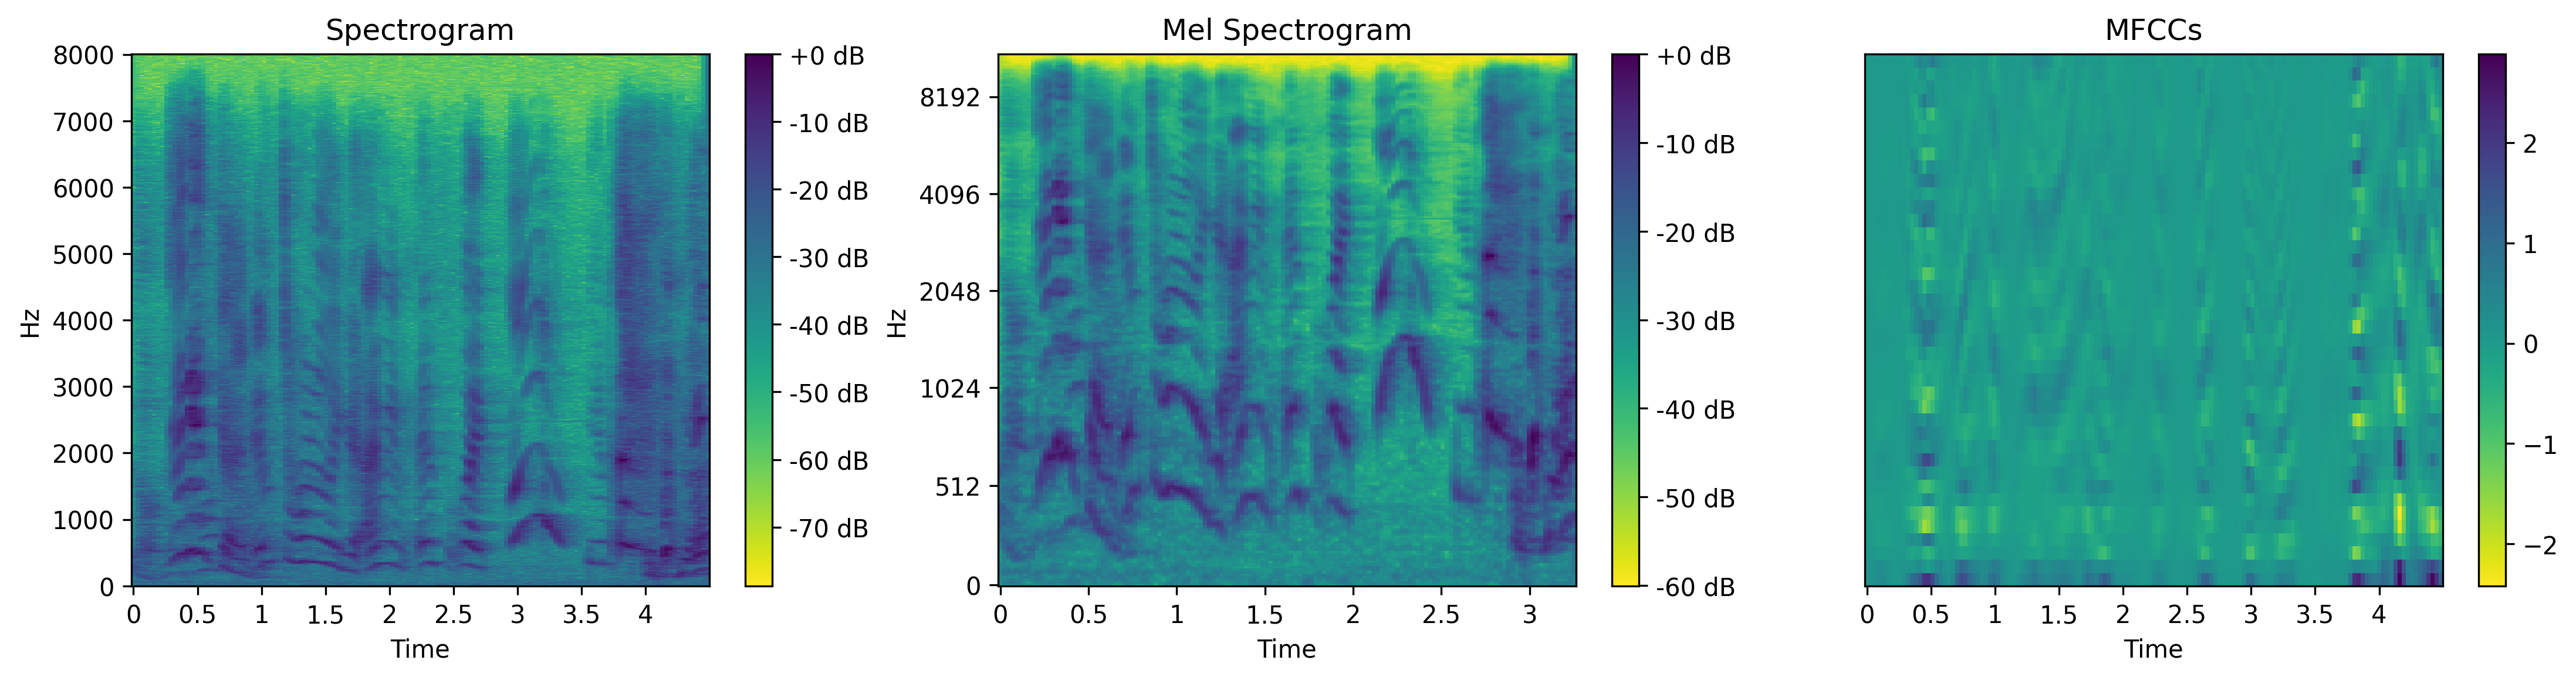
\includegraphics[width=\textwidth]{figs/4_4_deep_learning/features.png}
	\label{fig:dl_features}
	\caption{Graphical representations of the features used as input for the \ac{dl} classifiers.}
\end{figure}



\subsection{Classifiers Evaluation and Selection}

\subsubsection{Evaluation Strategy}

The classifiers were trained using a Tesla P4 GPU on the Google Colab service. To evaluate the performance of the classifiers, 5-fold cross-validation was performed using the stratified K-fold strategy to preserve the percentage of samples for each class. The models were trained for 80 epochs, with a batch size of 128 and a learning rate decay of 10\% every 10 epochs. The Adam optimizer was used for all models with a learning rate of 0.001.

The evaluation of the classifiers was done based on various metrics including accuracy, precision, recall, and macro F1-score. The training time was also annotated and the corresponding confusion matrices were also plotted, present in the appendix \ref{METER DPS}. These metrics were computed using the average across the 5 folds, without using class weights, to give an overall performance overview of the classifier.

\subsubsection{Numeric Data Classification}


\subsubsection{Image Classification}

In our study of deep learning-based \ac{ser} using images, we utilized transfer learning techniques with three different pre-trained models: ResNet50, VGG16, and Xception.

ResNet50, VGG16, and Xception are popular deep convolutional neural networks (CNN) that have shown outstanding performance in various computer vision tasks, including image classification. We used the pre-trained versions of them on the large-scale ImageNet dataset, which contains millions of labeled images belonging to thousands of different classes. This means their weights and biases have already been adjusted for the ImageNet dataset, and they have learned how to extract meaningful features from images, which helps improve the accuracy and generalization ability of the models, as it allows them to recognize patterns and shapes that are common across a wide range of images.

To prepare the data for these models, we loaded the images with a dimension of $224x224x3$ using the TensorFlow Keras \textit{load\_img} function from the \textit{preprocessing.image} module. The images were then converted into arrays using the \textit{img\_to\_array} function from the same module. In addition, before inputting the data into the models, we applied the respective preprocessing technique for each classifier. For example, we used the \textit{preprocess\_input} function from the Tensorflow  Keras \textit{applications.resnet50} module for the ResNet50 classifier.

In the transfer learning technique, all layers of the chosen classifier were frozen, and a new Dense layer with 64 units with \textit{relu} activation was added to the model. A Dropout layer with a 0.5 rate was then included to avoid overfitting, followed by a Dense layer with 4 units with \textit{softmax} activation to output the predicted emotion.

Through the implementation of these pre-trained models with transfer learning, we aim to harness their robust feature extraction abilities and significantly reduce the training duration required for the inherently computationally intensive 3D classification task at hand.


\subsubsection{Results and Conclusions}

Table \ref{tab:dl_models} displays the results obtained. The outcomes of the experiments illustrate the efficacy of employing transfer learning with pre-trained models for the task of \ac{ser}. While the spectrogram image feature attained the highest average accuracy when utilizing the Resnet50 model and weights, the mel spectrogram feature achieved the best overall performance across all models. Furthermore, the image of the mel spectrogram obtained the second-highest accuracy with the Resnet50 model and displayed a smaller standard deviation, indicating that it performed comparably well in all cross-validation folds.

From these results, we noted the Resnet50 model with Spectrogram Images as input as the best deep learning candidate as it obtained the highest values on all metrics.

\begin{table}[H]
	\centering
	\caption{\ac{dl} classification models performance on \ac{iemo}.}
	\label{tab:dl_models}
	\resizebox{\textwidth}{!}{%
		\begin{tabular}{llrrrrrr}
			\toprule
			Feature & Model & Accuracy & Macro F1 & Precision & Recall & \ac{mcc} & Training Time\\
			\midrule
			
			Spectrogram Image & Resnet50 & 58.24$\pm$2.20 & 58.97 & 59.38 & 59.00 & 0.436 & 1047.72 \\
			
			Mel Spectrogram Image & Resnet50 & 57.95$\pm$1.36 & 58.71 & 59.27 & 58.49 & 0.430 & 1133.66 \\
			
			MFCCs Image & Resnet50 & 56.59$\pm$0.45 & 57.29 & 58.59 & 56.67 & 0.410 & 1044.96 \\
			
			Mel Spectrogram Image & VGG16 & 55.07$\pm$2.23 & 55.82 & 56.77 & 55.29 & 0.389 & 1027.24 \\
			
			MFCCs Image & VGG16 & 54.73$\pm$1.47 & 55.51 & 56.32 & 55.14 & 0.386 & 1032.96 \\
			
			Spectrogram Image & VGG16 & 54.28$\pm$0.90 & 55.21 & 55.85 & 54.87 & 0.379 & 1147.05 \\
			
			Mel Spectrogram Image & Xception & 53.10$\pm$1.42 & 53.84 & 54.27 & 53.68 & 0.364 & 1171.14 \\
			
			MFCCs Image & Xception & 52.78$\pm$0.96 & 53.47 & 54.10 & 53.22 & 0.359 & 1181.58 \\
			
			Spectrogram Image & Xception & 52.78$\pm$1.54 & 53.51 & 53.48 & 53.62 & 0.361 & 1190.07 \\
			
			Spectrogram & 2D-CNN & 50.12$\pm$0.91 & 50.04 & 52.98 & 49.65 & 0.320 & 3167.14 \\
			
			Mel Spectrogram & 2D-CNN \& LSTM & 48.02$\pm$1.14 & 47.93 & 48.60 & 48.47 & 0.298 & 1427.02 \\
			
			MFCCs & 2D-CNN & 46.70$\pm$0.85 & 47.13 & 49.53 & 46.75 & 0.275 & 303.49 \\
			
			Spectrogram & 2D-CNN \& LSTM & 46.01$\pm$1.77 & 47.09 & 47.37 & 46.87 & 0.269 & 5413.99 \\
			
			MFCCs & 2D-CNN \& LSTM & 45.56$\pm$1.15 & 46.26 & 46.29 & 46.25 & 0.263 & 298.06 \\
			
			Mel Spectrogram & 2D-CNN & 32.51$\pm$1.13 & 21.34 & 20.38 & 30.26 & 0.102 & 1166.9 \\		
			
			
			\bottomrule
		\end{tabular}%
	}
\end{table}

\section{Classifiers Results}

In this section, we present and analyze the results of the best candidate models obtained from both the traditional and \ac{dl}-based \ac{ser} approaches.

The top-performing model from the traditional approach is an \ac{xgb} classifier, utilizing 33 audio features as input. This model achieved an accuracy of 60.69\% after performing 5-fold \ac{cv} on the \ac{iemo} dataset. On the other hand, the final model obtained from the \ac{dl} approach is a Resnet50 model, which uses audio spectrogram images as input. This model achieved an accuracy of 58.24\% using the same evaluation strategy and dataset.


\subsection{Models Cross-Dataset Validation}

The performance of the final models trained using the \ac{iemo} dataset and tested on three different datasets, namely eNTERFACE'05, EMO-DB, and CREMA-D, are presented in Table \ref{final_models}. The cross-dataset validation was performed to evaluate the generalization capabilities, robustness, and significance of trained models. By testing the models on datasets with different recording conditions, language, and emotional expression variability, we can assess their ability to generalize to new, unseen data. This is an important step towards creating robust \ac{ser} models that can be applied in real-world scenarios where the training data may not perfectly match the test data.


\begin{table}[H]
	\centering
	\caption{Final models trained on \ac{iemo} and evaluated on different datasets.}
	\label{final_models}
	\resizebox{\textwidth}{!}{%
		\rowcolors{2}{gray!25}{white}
		\begin{tabular}{llrrrrrr}
			\toprule
			Dataset & Model & Accuracy & Macro F1 & Precision & Recall & \ac{mcc} & Time \\
			\midrule
			\addlinespace[1mm]
			
			eNTERFACE'05 & Traditional & 32.22 & 17.25 & 29.09 & 24.17 & 0.08 & 0.17 \\
			& \acl{dl} & 36.67 & 22.91 & 44.36 & 27.50 & 0.087 & 0.25 \\
			
			\midrulec
			\addlinespace[1mm]
			
			EMO-DB & Traditional & 38.35 & 15.82 & 14.80 & 26.06 & 0.07 & 0.10 \\
			& \acl{dl} & 38.35 & 15.79 & 37.78 & 25.99 & 0.066 & 0.18 \\ 
			
			\midrulec
			\addlinespace[1mm]
			
			CREMA-D & Traditional & 45.22 & 38.96 & 47.62 & 46.41 & 0.3151 & 0.10 \\
			& \acl{dl} & 54.14 & 47.71 & 51.68 & 52.98 & 0.407 & 0.30 \\
			
			
			\bottomrulec
		\end{tabular}%
	}
\end{table}


The \ac{dl} model generally outperformed the traditional model on all datasets, except for the EMO-DB dataset, where they performed similarly. The best overall performance was achieved on the CREMA-D dataset, with the \ac{dl} model achieving an accuracy of 54.14\% and a macro F1 score of 47.71\%.

However, both models exhibited poor results on the eNTERFACE'05 and EMO-DB datasets, with accuracy scores of less than 40\%, and, in terms of macro f1-scores they are slightly better for the eNTERFACE'05 but still low. A low macro F1 score means that the model's ability to correctly classify instances of different classes is poor. This could be due to several factors, such as class imbalance or the model's inability to capture important features that distinguish between different classes.

In terms of computation time, the traditional models were faster than the \ac{dl} models, which is evident from the lower time values in the table. This is a crucial factor when employing these models for real-time emotion recognition systems.

Further insights into the obtained results can be obtained through the confusion matrices, as shown in Figure \ref{fig:final_cm}. We can observe both models predicted the anger emotion multiple times across all three datasets. In the case of the eNTERFACE'05 dataset, which lacks neutral emotions, the \ac{dl} model predicted the happiness emotion more frequently compared to the traditional model, which is the leading reason for the slightly better results.

Analyzing the confusion matrix of the EMO-DB dataset, it is clear that the anger emotion was predicted for the majority of audio files, which is likely due to the German language used in the dataset known for its assertiveness and directness. However, this should not be interpreted as a flaw in the model's performance but rather a reflection of the language's characteristics used in the training and testing datasets. This highlights the English language bias of our \ac{ser} models and suggests that the results for other languages may not be satisfactory.

Moreover, the traditional model had difficulty recognizing the happiness emotion in the CREMA-D dataset, as in the eNTERFACE'05 dataset, and often confused the neutral emotion with sadness. Although the \ac{dl} model exhibited the same confusion, it predicted the sadness emotion more often.

Finally, it is worth noting that the traditional models were faster than the \ac{dl} models, with lower time values in the table, which is critical when implementing these models for real-time \ac{ser} systems.

In conclusion, the results suggest that the \ac{dl} model may be more suitable for the \ac{ser} task on diverse datasets, owing to its improved feature extraction and generalization abilities. However, the \ac{dl} model is slower compared to the traditional models, which can significantly impact real-time applications. Furthermore, we recommend that these models should be utilized for English-spoken audio recordings and preferably with less prominent accents, to minimize any language bias-induced errors.


\begin{figure}[H]
	\begin{subfigure}{.5\textwidth}
		\centering
		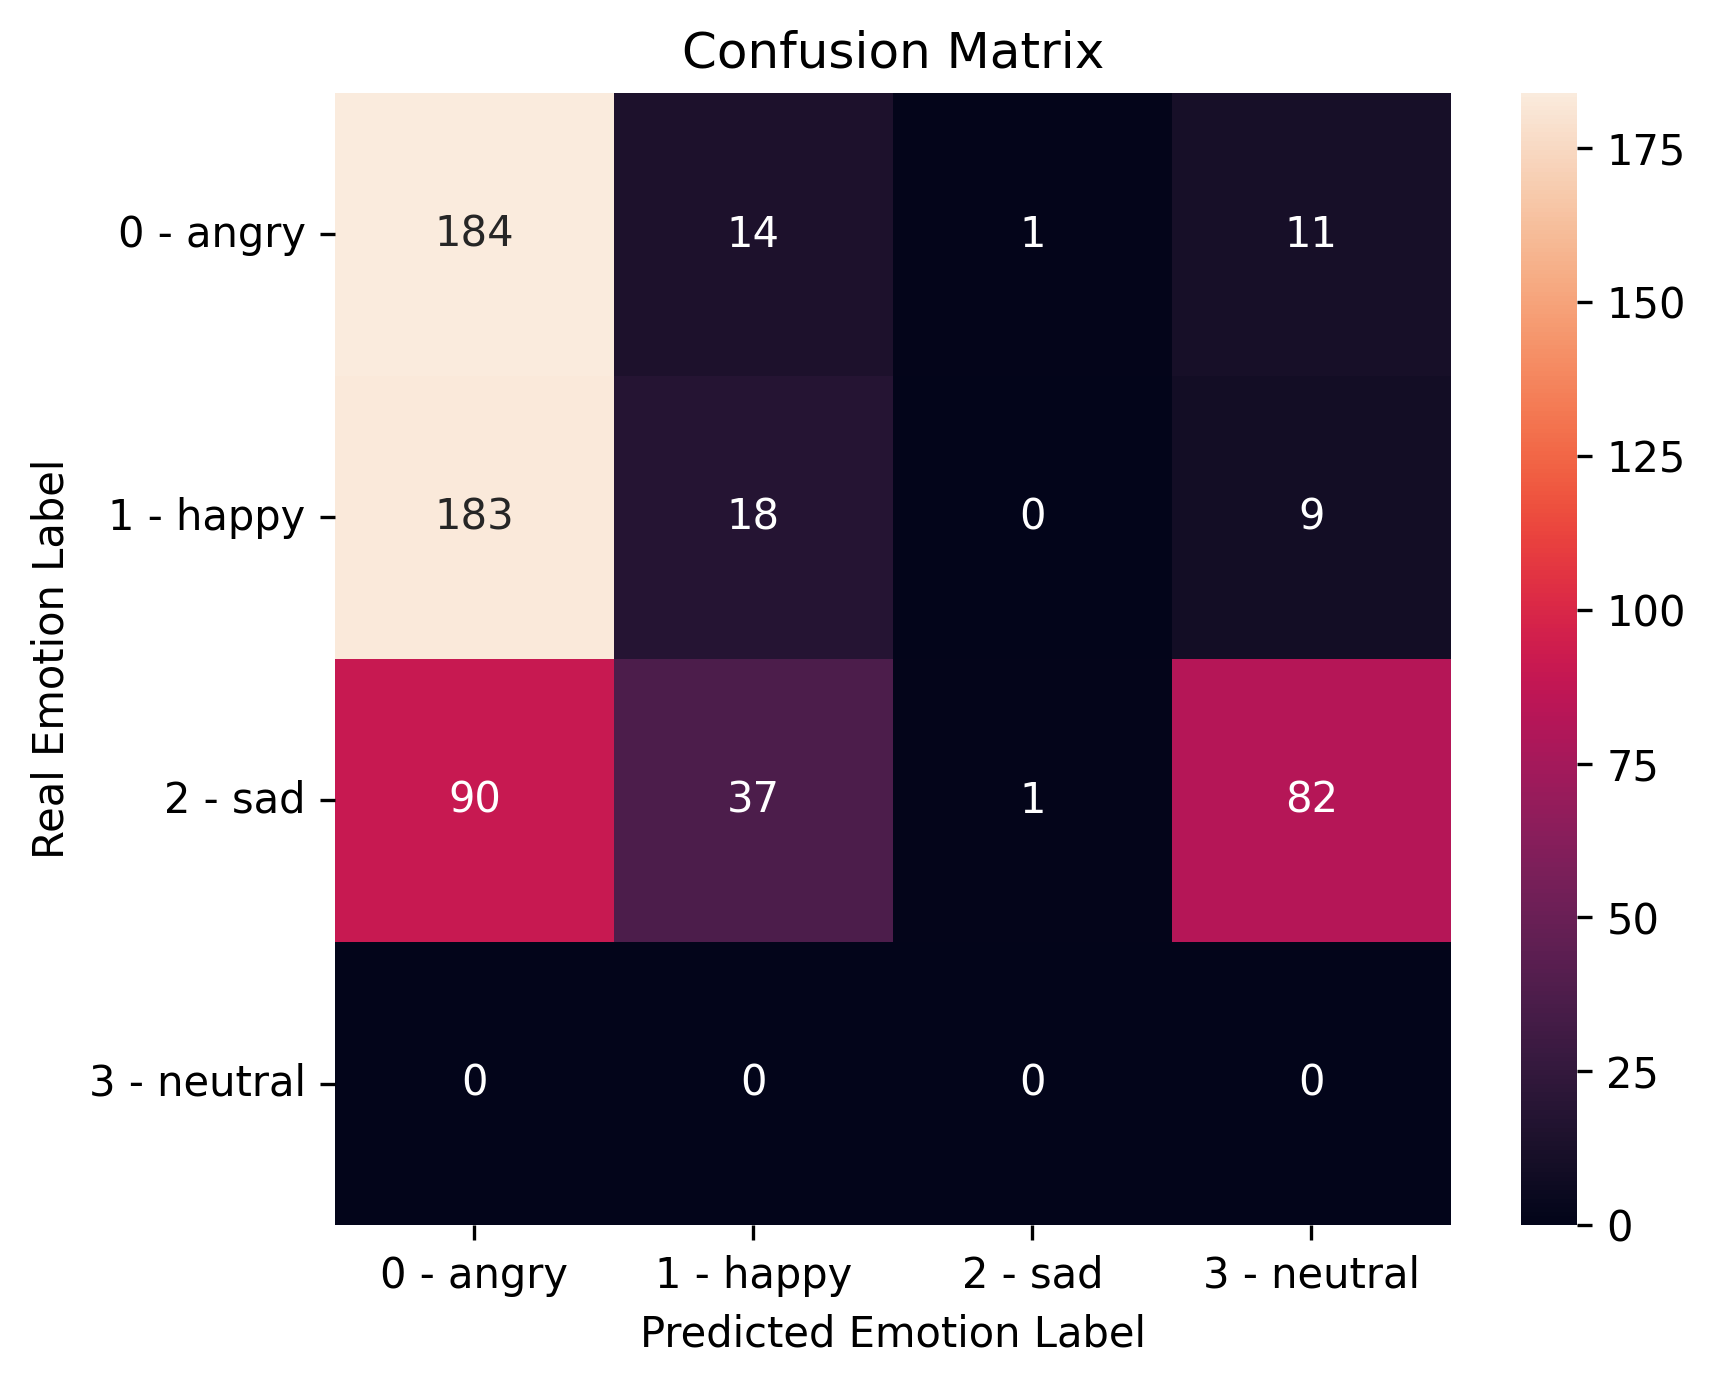
\includegraphics[width=\linewidth]{figs/4_5_discussion/ent_trad_cm.png}
		\caption{eNTERFACE'05 traditional model confusion matrix.}
	\end{subfigure}%
	\begin{subfigure}{.5\textwidth}
		\centering
		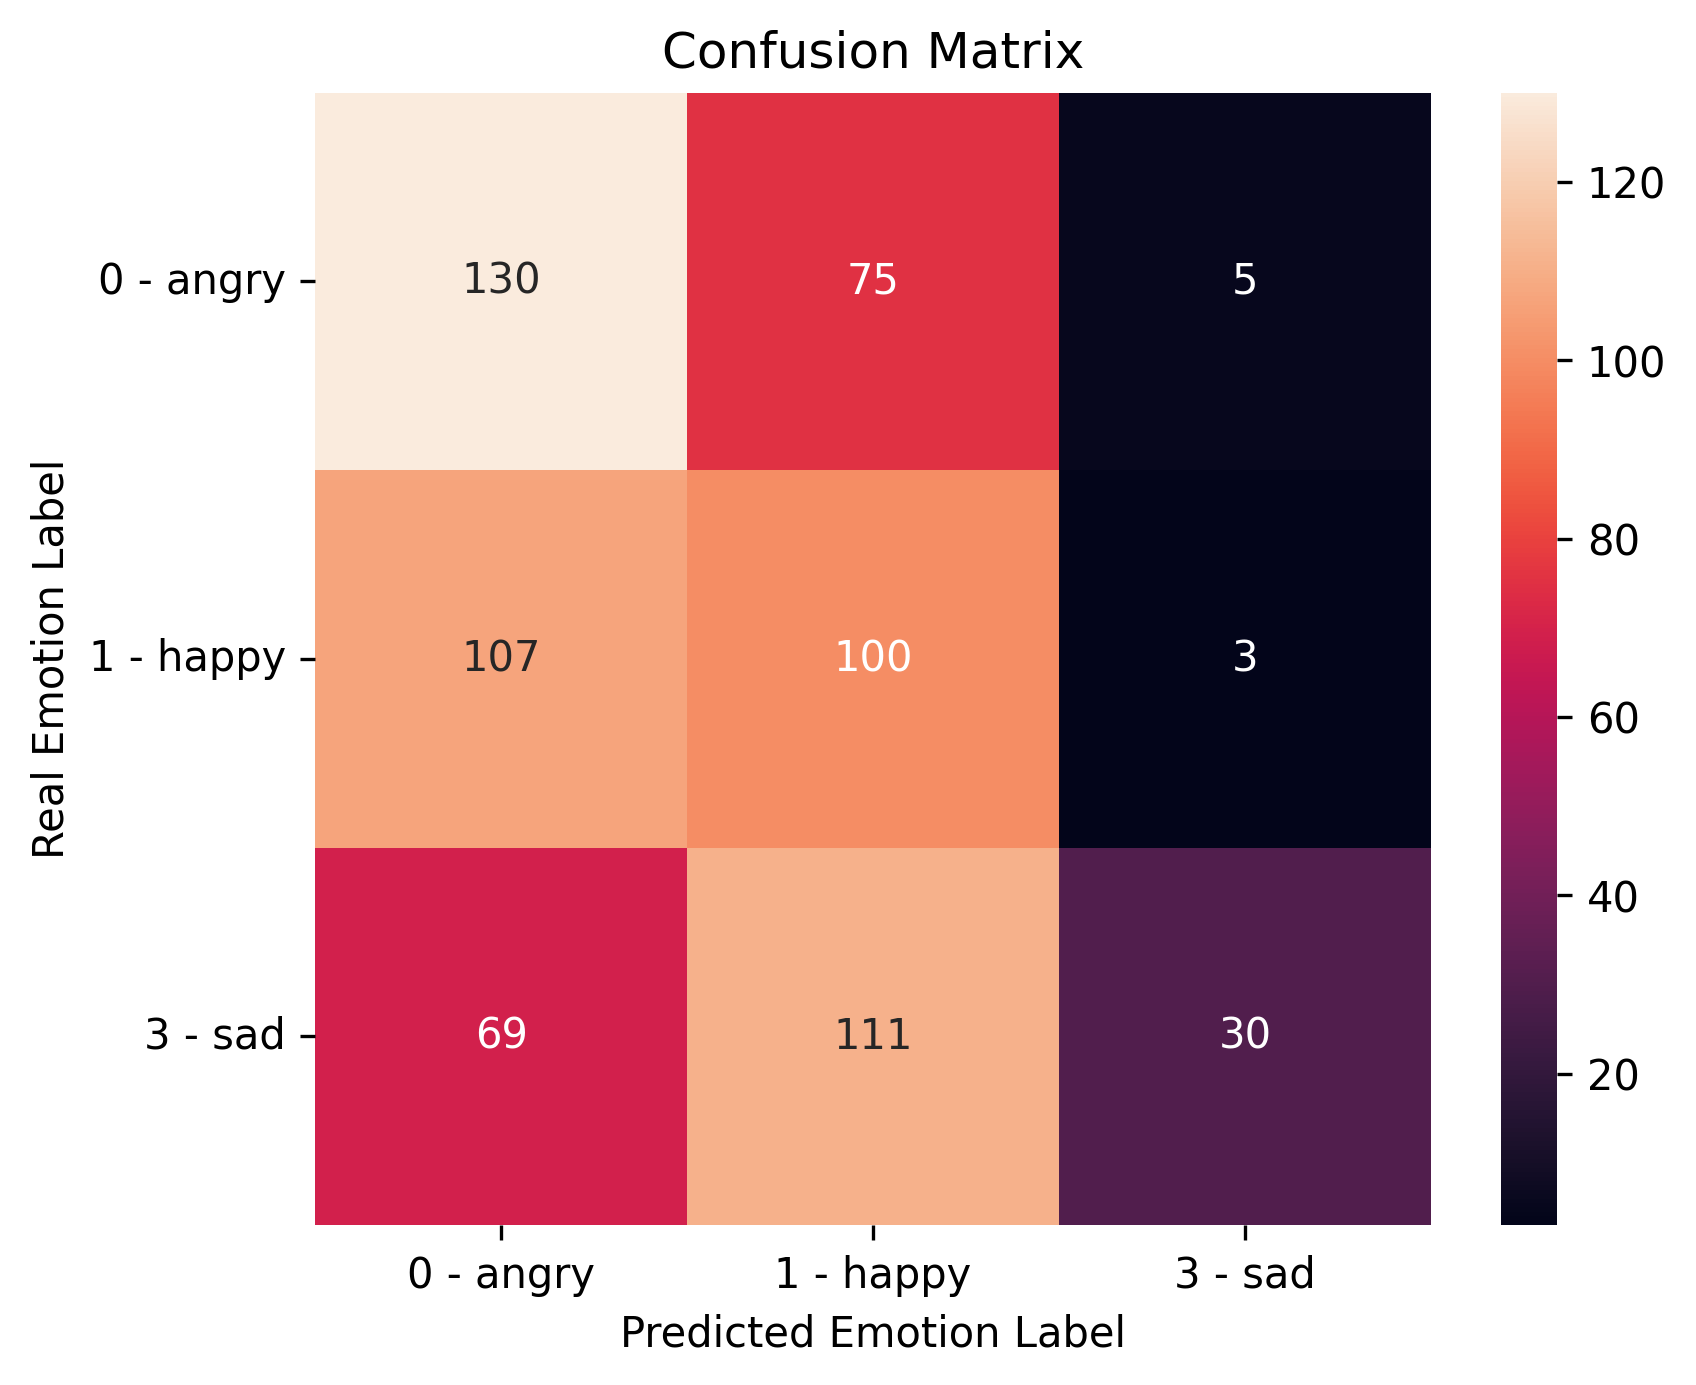
\includegraphics[width=\linewidth]{figs/4_5_discussion/ent_deep_cm.png}
		\caption{eNTERFACE'05 \ac{dl} model confusion matrix.}
	\end{subfigure}
	\newline
	\begin{subfigure}{.5\textwidth}
		\centering
		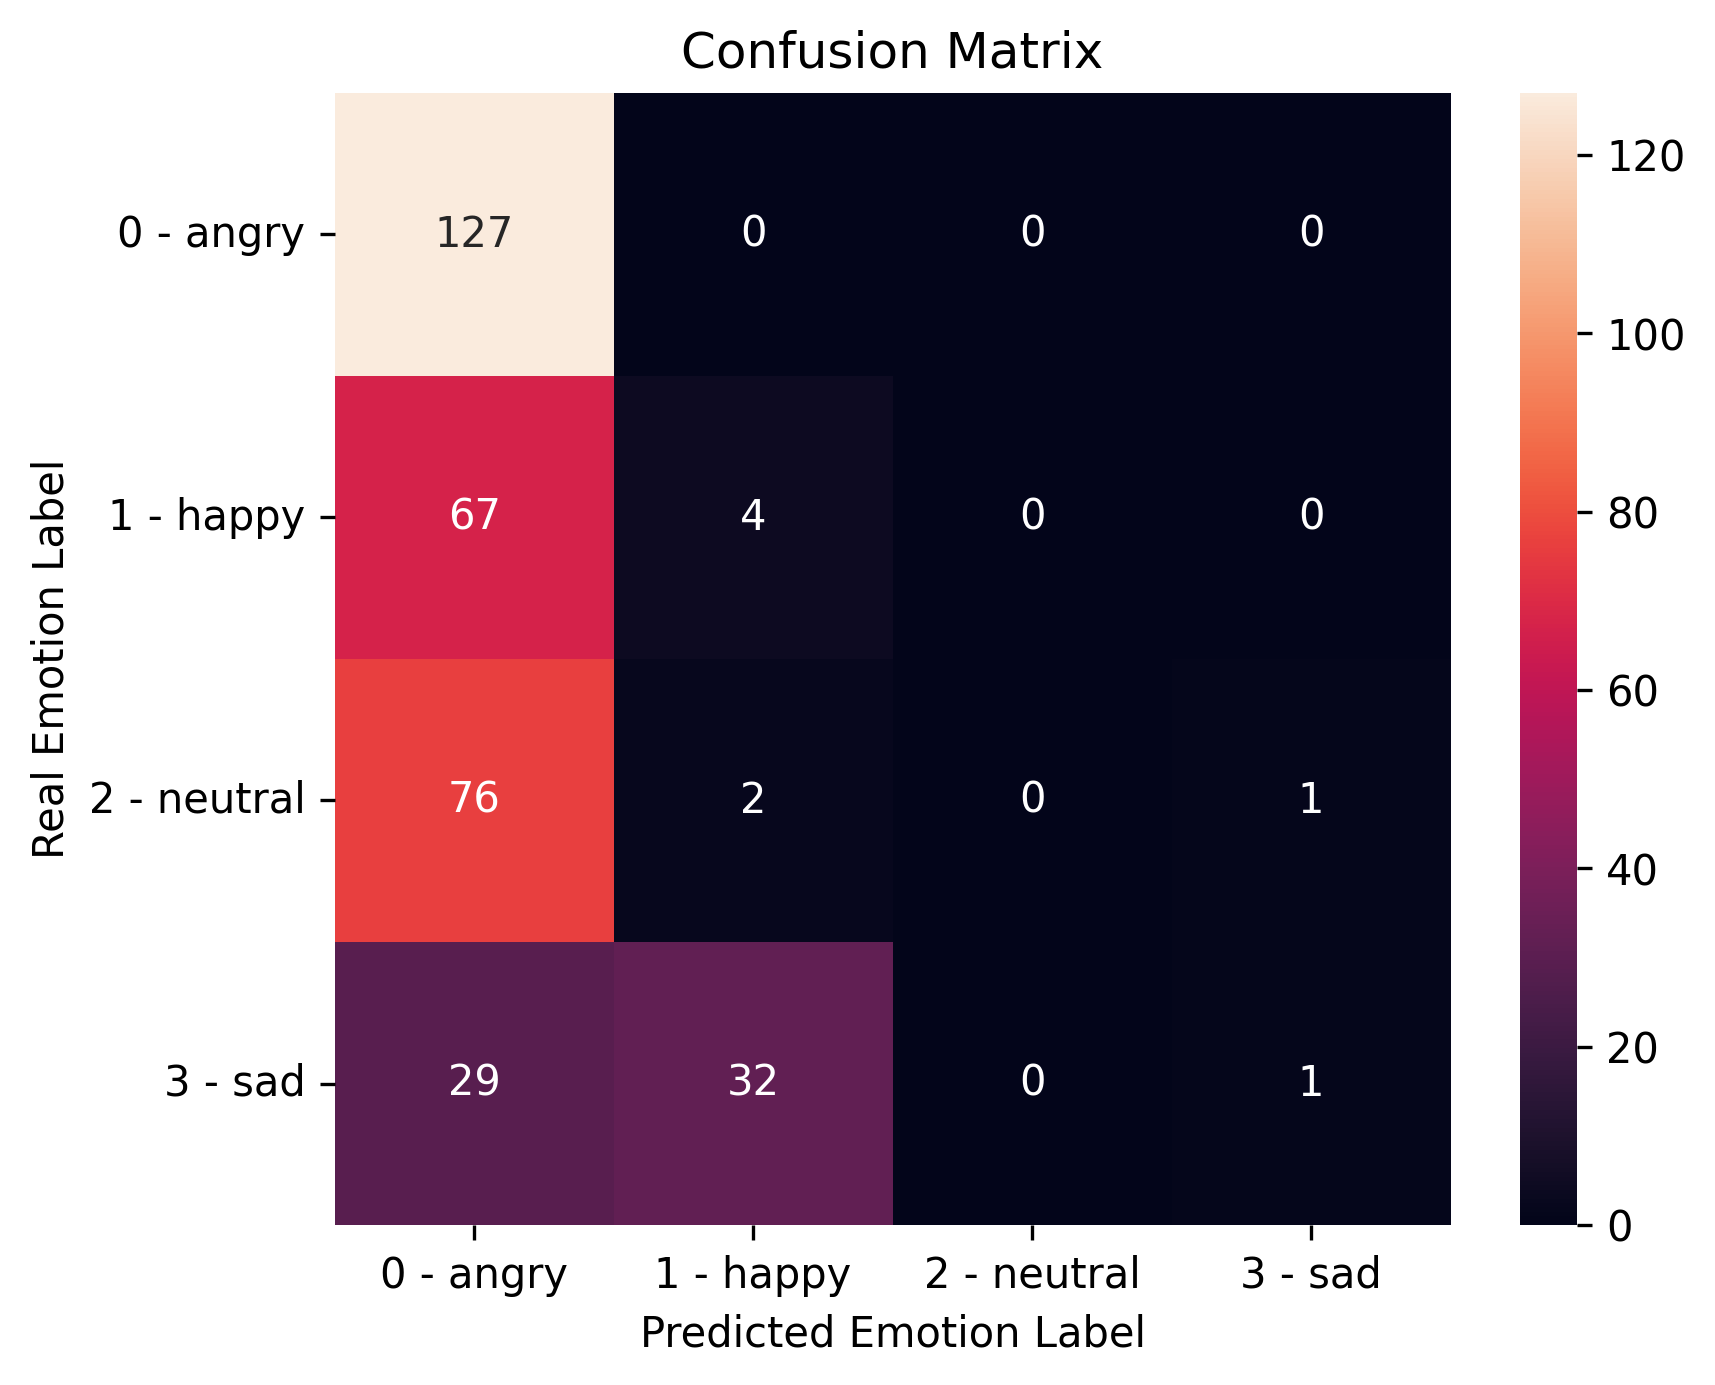
\includegraphics[width=\linewidth]{figs/4_5_discussion/emo_trad_cm.png}
		\caption{EMO-DB Traditional model confusion matrix.}
	\end{subfigure}%
	\begin{subfigure}{.5\textwidth}
		\centering
		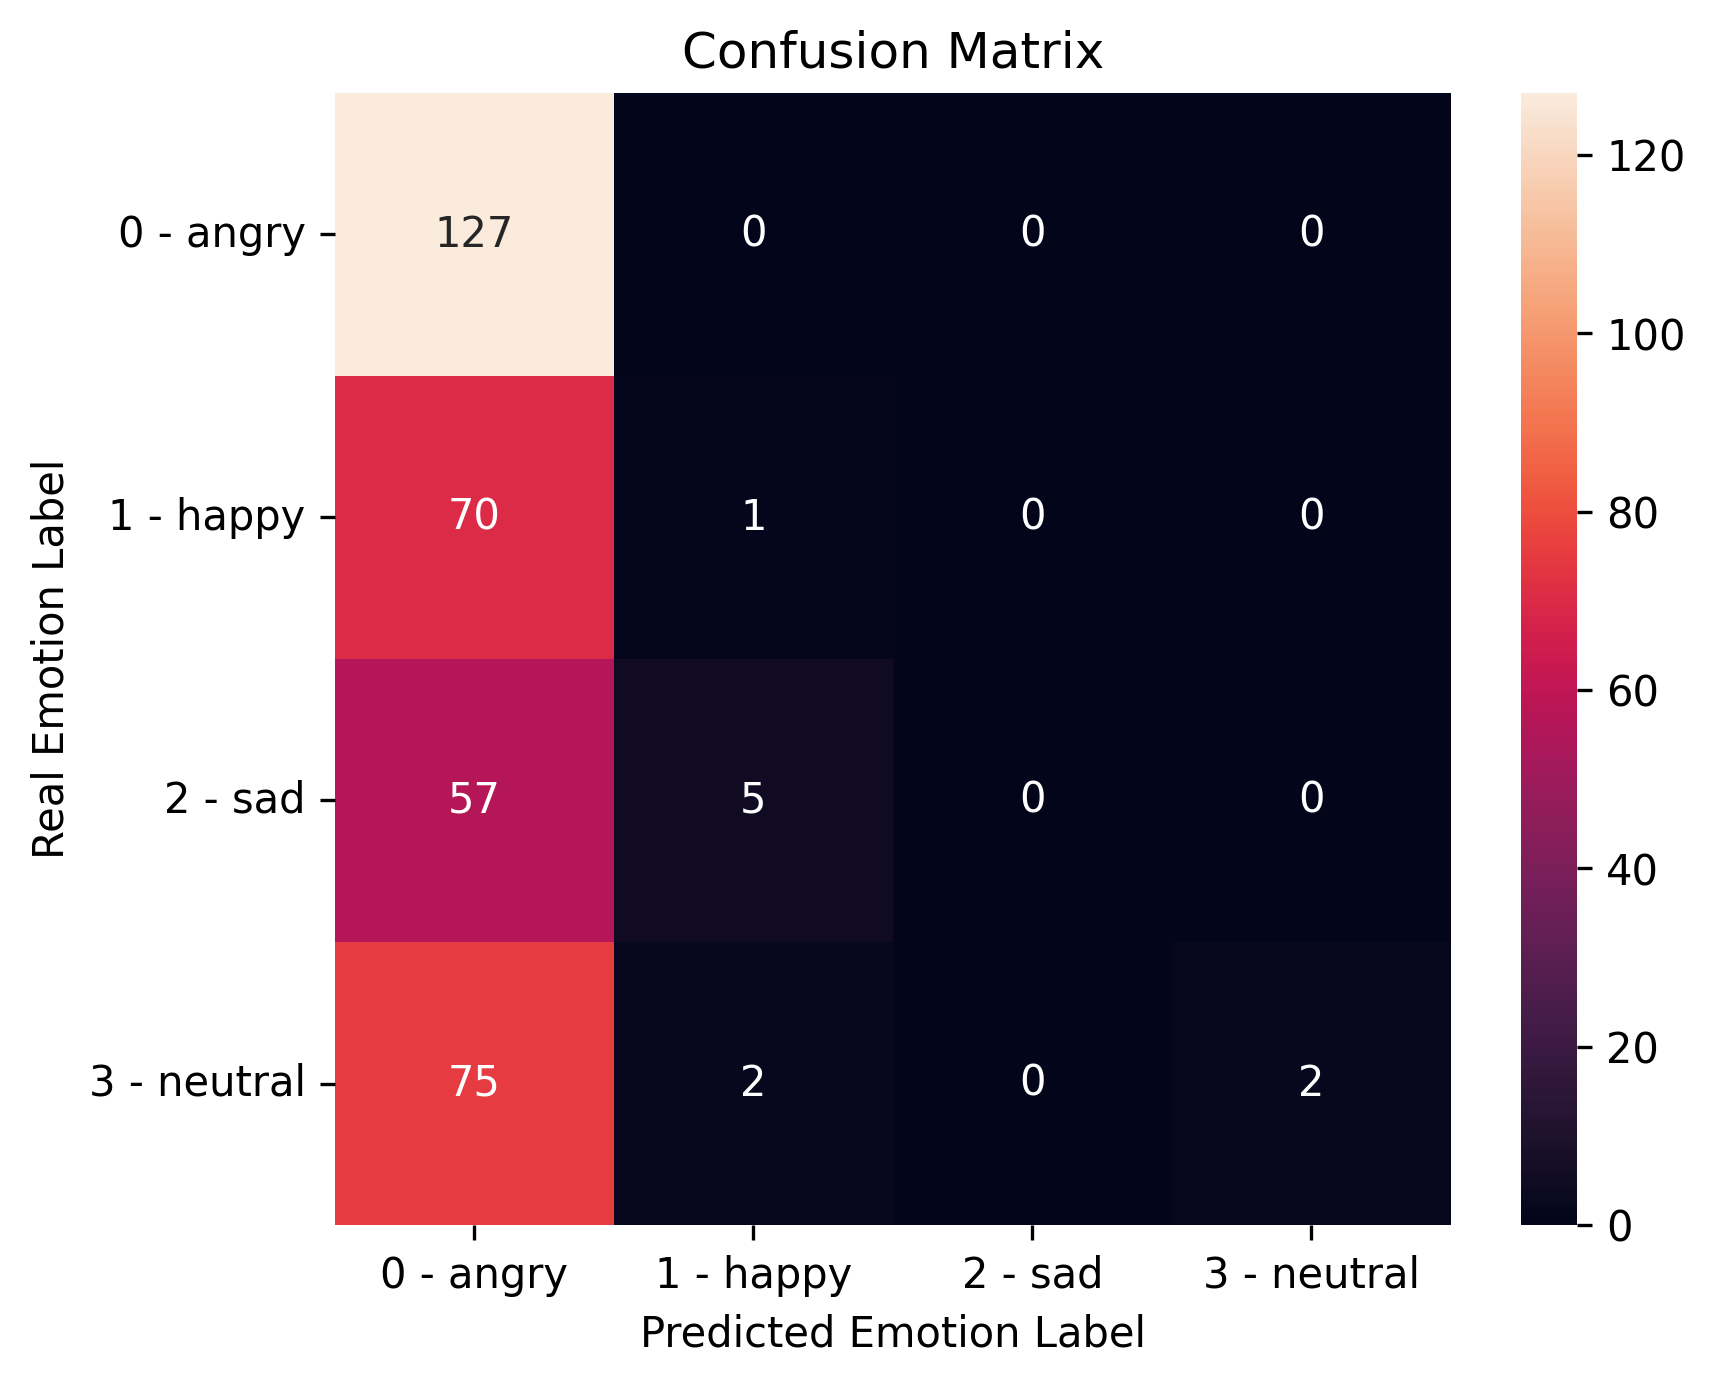
\includegraphics[width=\linewidth]{figs/4_5_discussion/emo_deep_cm.png}
		\caption{EMO-DB \ac{dl} model confusion matrix.}
	\end{subfigure}
	\newline
	\begin{subfigure}{.5\textwidth}
		\centering
		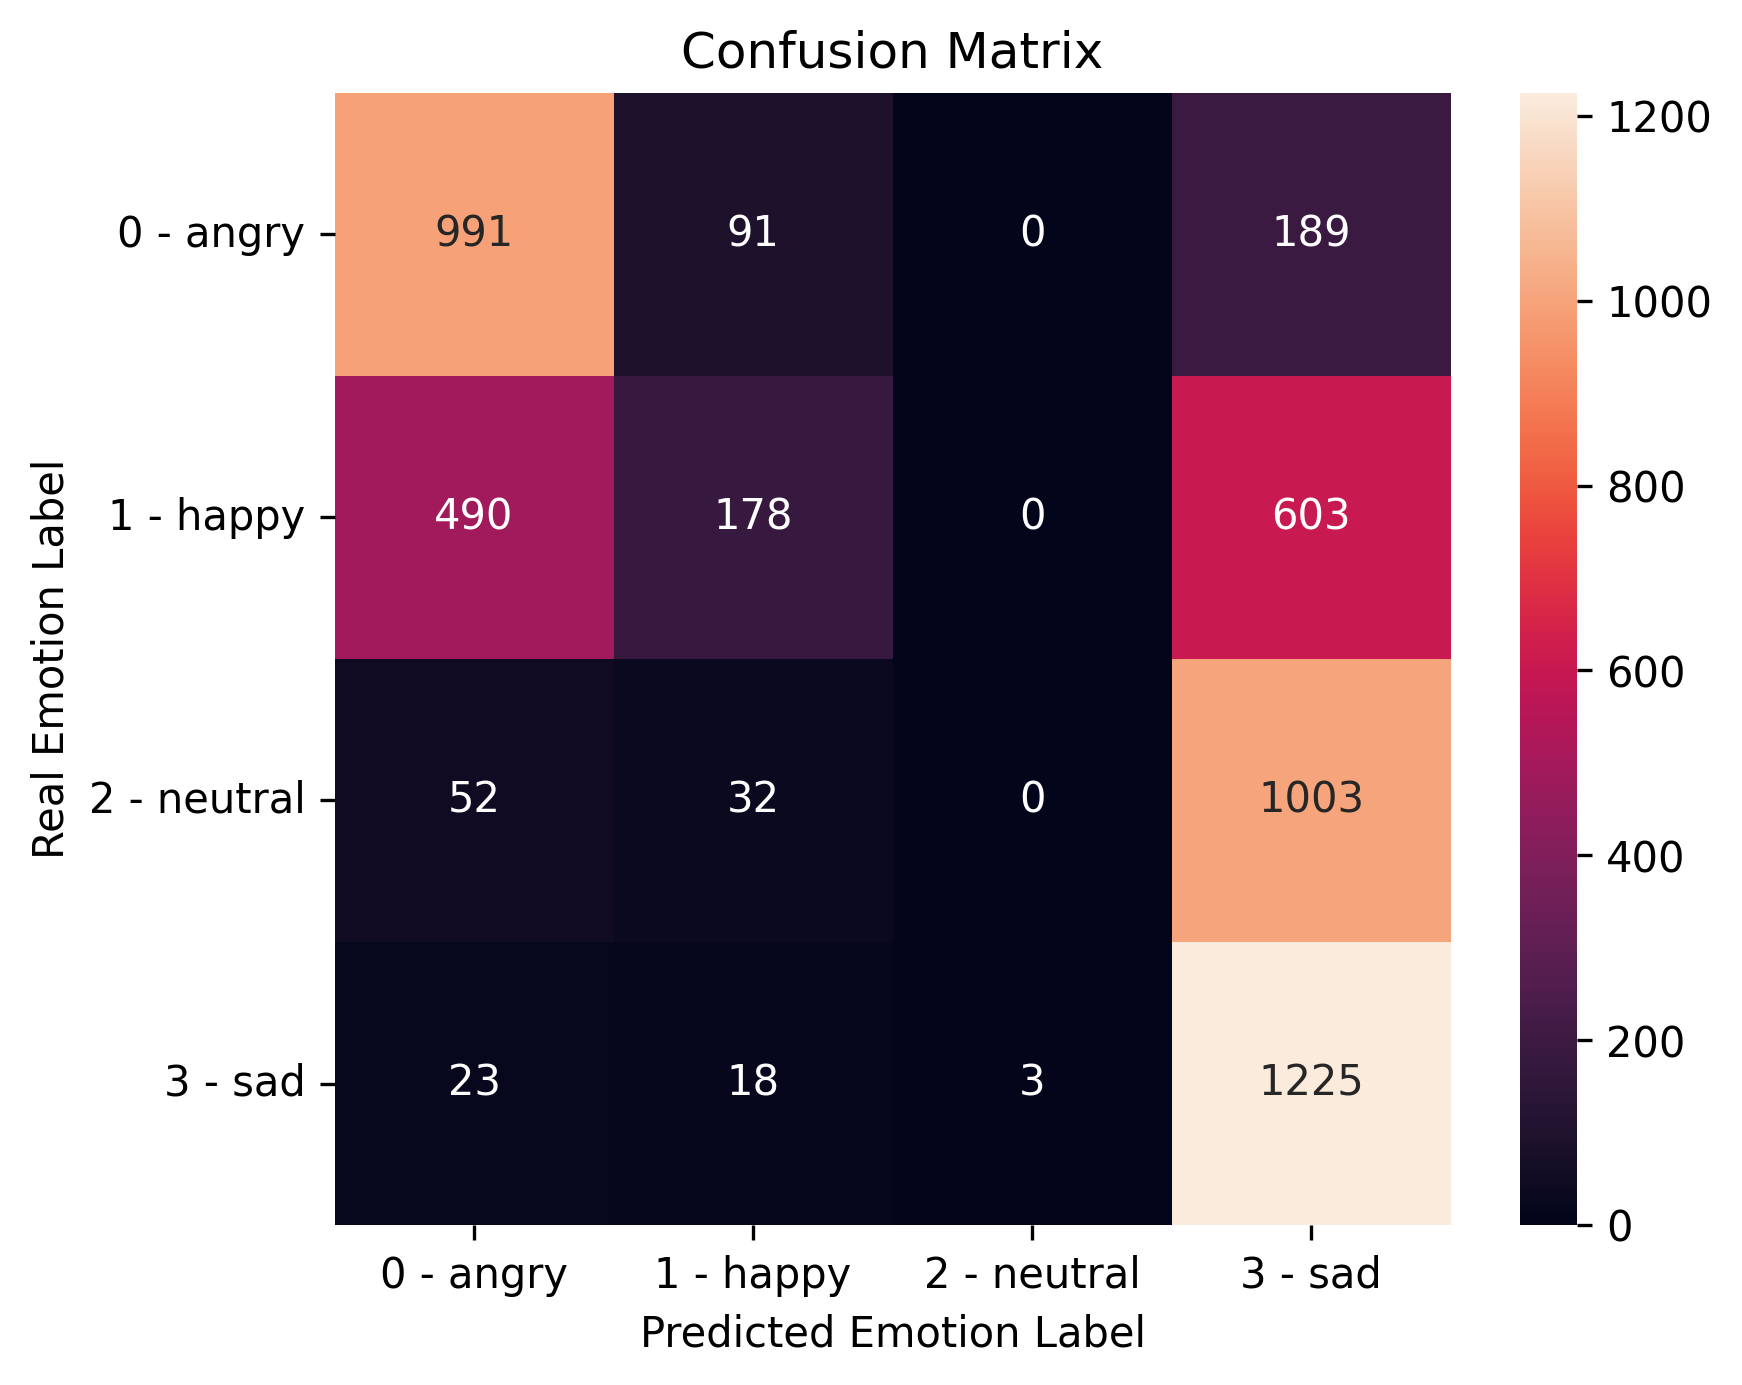
\includegraphics[width=\linewidth]{figs/4_5_discussion/cre_trad_cm.png}
		\caption{CREMA-D Traditional model confusion matrix.}
	\end{subfigure}%
	\begin{subfigure}{.5\textwidth}
		\centering
		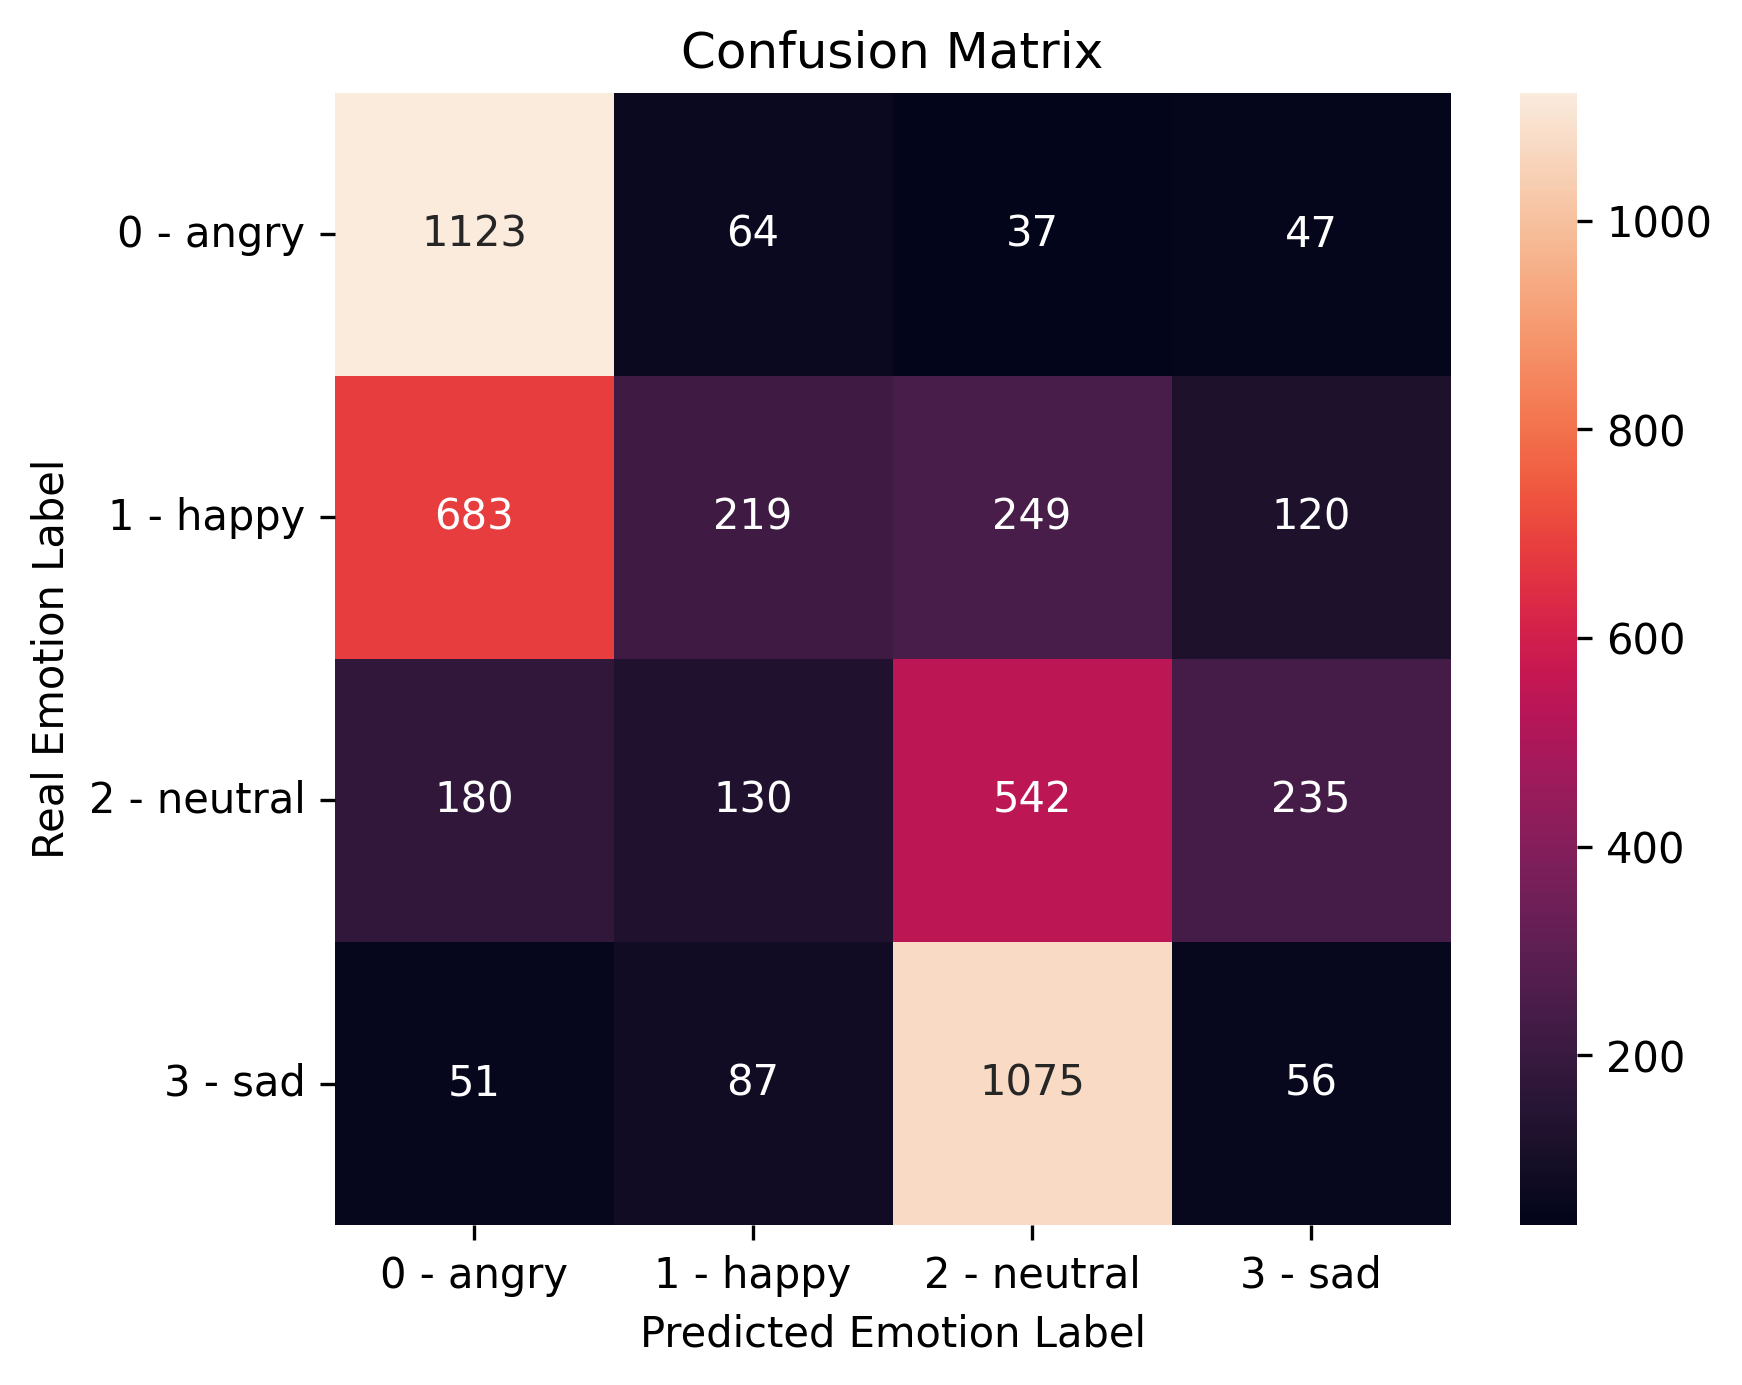
\includegraphics[width=\linewidth]{figs/4_5_discussion/cre_deep_cm.png}
		\caption{CREMA-D \ac{dl} model confusion matrix.}
	\end{subfigure}
	\caption{Final models confusion matrices on the eNTERFACE'05, EMO-DB and CREMA-D datasets.}
	\label{fig:final_cm}
\end{figure}


\subsection{\ac{sota} Comparison}

In Table \ref{tab:modelssoa}, we summarize the performance of various classification models on the \ac{iemo} dataset, including our proposed model (highlighted in blue). The first four rows represent traditional feature-based approaches, while the remaining rows represent \ac{dl}-based approaches.

It is important to note that the \ac{sota} results are not always directly comparable, as different authors may use different subsets of data and evaluation methodologies. For instance, some authors may not consider the emotion of excitement as happiness, others may only use improvised data and not scripted, or even perform different validation methods such as 10-fold \ac{cv}. Additionally, the random seeds for the k-fold splits may also impact the final classification performance.

Our proposed model, an \ac{xgb} classifier utilizing 33 audio features, achieved an accuracy of 60.69\% on 5-fold \ac{cv}, outperforming the traditional approaches presented in the first three rows. Another model from the traditional approach, that outperformed ours, utilized a \ac{cnn} for its feature extraction capabilities; however, we still consider it traditional as the authors still performed feature extraction to obtain the 193-dimensional feature vector for the model's input.

Among the \ac{dl}-based approaches, our Resnet50 model achieved an accuracy of 58.24\%, which is lower than the other \ac{sota} results. The Quaternion \ac{cnn} achieved the highest accuracy of 70.46\%, utilizing a unique approach of encoding the Mel spectrogram in an RGB quaternion domain, which may have contributed to its higher accuracy.

\begin{table}[H]
	\centering
	\caption{\ac{sota} \ac{ser} classification models performance on \ac{iemo}.}
	\label{tab:modelssoa}
	\resizebox{\textwidth}{!}{%
		\begin{tabular}{lccr}
			\toprule
			Model                      & Input & Evaluation Strategy & Accuracy (\%) \\
			\toprulec
			\rowcolor{gray!25}
			\multicolumn{4}{c}{Traditional Feature-Based \ac{ser} Approaches} \\
			\midrulec
			
			\begin{tabular}[l]{@{}l@{}}Ensemble of \ac{rf}, \ac{xgb}\\and Multilayer Perceptron\end{tabular} \cite{HandCraftedSahu} & \begin{tabular}[c]{@{}c@{}}8-dimensional audio\\features vector\end{tabular} & \begin{tabular}[c]{@{}c@{}}1 random 80:20\\train-test split\end{tabular} & 56.00 \\
			\addlinespace[1mm]
			
			\begin{tabular}[l]{@{}l@{}}Multi-level binary\\decision trees \cite{Lee2011}\end{tabular} & 384 audio features vector & 10 fold \ac{cv} & 58.46 \\
			\addlinespace[1mm]
			
			\rowcolor{LightCornflowerBlue}
			\ac{xgb} [Ours] & 33 audio features vector & 5-fold \ac{cv} & 60.69 \\
			\addlinespace[1mm]
			
			\ac{cnn} \cite{Issa2020}  & 193 audio features vector & 5-fold \ac{cv} & 64.30 \\
			\addlinespace[1mm]
			
			\toprulec
			\rowcolor{gray!25}
			\multicolumn{4}{c}{\acl{dl}-Based \ac{ser} Approaches} \\
			\midrulecb
			
			\rowcolor{LightCornflowerBlue}
			Resnet50 [Ours] & 3-D Spectrogram Image & 5-fold \ac{cv} & 58.24 \\
			\addlinespace[1mm]
			
			\ac{cnn} and \ac{rnn} \cite{ma18b_interspeech} & Log-Spectrogram & 5-fold \ac{cv} & 64.22 \\
			\addlinespace[1mm]
			
			\begin{tabular}[l]{@{}l@{}}3-D attention-based\\convolutional \ac{rnn} \cite{8421023}\end{tabular} & 3-D Mel-Spectrogram Image & 10-fold \ac{cv} & 64.7 \\
			\addlinespace[1mm]
			
			\begin{tabular}[l]{@{}l@{}}\ac{cnn} and \ac{lstm}\\with attention \cite{Zhao2019}\end{tabular} & Mel-Spectrogram & 5-fold \ac{cv} & 67.0 \\
			\addlinespace[1mm]
			
			Quaternion \ac{cnn} \cite{Muppidi2021} & \begin{tabular}[c]{@{}c@{}}Mel spectrogram\\ encoded in an RGB\\quaternion domain\end{tabular} & 5-fold \ac{cv} & 70.46 \\
			\addlinespace[1mm]
			
			\bottomrule
		\end{tabular}%
	}
\end{table}

\section{Discussion}

In this chapter, we selected the \ac{iemo} dataset for training and testing our models. The dataset contains emotional speech data from 10 actors performing scripted and improvised scenarios, with each recording labeled with four different emotions: anger, happiness, sadness, and neutral. We chose this dataset because of its high-quality recordings, its availability, and its popularity in the \ac{sota}. To evaluate the generalization capability of our models, we also selected three additional datasets to perform cross-dataset evaluation: eNTERFACE'05, EMO-DB, and CREMA-D. These datasets provide a diverse set of challenges for our models, including variations in speech content, recording conditions, and emotional expressions, making them suitable for evaluating the robustness of our models to different scenarios.

Afterwards, we applied a set of audio preprocessing techniques to the audio data, and reached a simple strategy that reduces background noises and trims the silence in the beginning and ending of the audios. This preprocessing step showed that it helps removing irrelevant information and reduce noise. However, the choice of preprocessing techniques may depend on the specific dataset and recording conditions, so we recommended researchers to experiment several preprocessing strategies to determine the most effective approach.

Our findings on the cross-dataset validation support the idea that the \ac{dl} model is better suited for \ac{ser} tasks on diverse datasets, due to its improved feature extraction and generalization capabilities of data under different factors. We believe this is mainly because the traditional approach relies on a feature input vector derived from the training dataset, limiting its applicability to other datasets. However, the traditional model is more suitable for real-time applications as it has a faster processing speed than the \ac{dl} model.

In addition, our \ac{xgb} model achieved competitive results compared to the \ac{sota} approaches presented in the table, despite using only a 1-dimensional 33 audio feature vector. This makes it more computationally efficient than other traditional approaches that require a much larger number of features. Nonetheless, both of our models still have the potential for improvement, especially in the \ac{dl} approach where fine-tuning was limited due to its computational expense. We also recommend using our models for English-spoken audio recordings with less prominent accents to mitigate language bias since the training dataset contains English audio.

Overall, this chapter offers a comprehensive implementation and thought process, along with conclusions and interpretations of the obtained results, laying a solid foundation for future research in developing more robust and accurate \ac{ser} models. It highlights the importance of considering the impact of different validation methodologies used in \ac{ser} research to ensure the models' robustness and applicability to diverse datasets. These findings contribute to the growing body of research on \ac{ser} and provide valuable insights for researchers and practitioners in the field.

\chapter{Data Stratification}
\label{chapter:data_stratification}


In order to better understand the properties of the data in the \ac{iemo} dataset, we performed stratification based on several attributes of the dataset. This stratification aimed to group similar data together and investigate their common properties, and, discover limitations that these properties pose to the machine learning model in the \ac{ser} area.

\section{Recordings Durations}

The duration of an audio recording can significantly impact the analysis and modeling of the data. Shorter recordings may not capture enough information to adequately represent the signal of interest, while longer recordings may contain irrelevant or redundant information.

We stratified the dataset based on the duration of the recordings. The dataset contains recordings ranging from approximately 0.25 to 34 seconds in duration, and we divided the recordings into three evenly balanced groups, in terms of the number of recordings: short, less than or equal to  2.29 seconds, medium, greater than 2.29 and less than or equal to 4.38 seconds, and long, greater than 4.38 seconds.

Table \ref{5:durations} presents the impact of the duration of the recordings on the performance of the chosen traditional AdaBoost model. The longest recordings have the highest performance, with an accuracy of 63.4\%, despite having more recordings than the medium duration data. 

\begin{table}[H]
	\centering
	\caption{Traditional model 5-fold cross-validation results based on the recordings' duration.}
	\label{5:durations}
	\begin{tabular}{lrlrrrr}
		\toprule
		Recordings Duration &   Total Data & Accuracy    &   Macro F1 &   Precision &   Recall &   MCC. \\
		\midrule
		Short ($]0, 2.29]$ s)	 	&      1844 & 57.38+-1.15 &   55.48 &  59.51 &  53.88 &  0.40  \\
		Medium ($]2.29, 4.38]$ s) 	&      1843 & 56.38+-1.26 &   56.81 &  57.34 &  56.73 &  0.41 \\
		Long ($]4.38, 34]$ s) 		&      1844 & 62.91+-1.69 &   63.31 &  63.91 &  63.11 &  0.50  \\
		
		
		\bottomrule
	\end{tabular}
\end{table}

The obtained classification results suggest that longer recordings are easier for the model to classify accurately, as they provide more information. This allows us to conclude that recordings' duration has a substantial performance impact on the \ac{ser} task and is a significant factor to consider when building classification models.

\section{Speaker Gender}

Another attribute we used for stratification was the gender of the speaker. The dataset contains a similar amount of recordings from both male and female speakers, having 2649 recordings with female speakers and 2882 with male speakers.

To evaluate the performance of the model on different genders, we trained and tested the model on recordings from female speakers, male speakers, and mixed-gender recordings. Table \ref{5:gender} shows the 5-fold cross-validation results of the model on each category.

\begin{table}[H]
	\centering
	\caption{Traditional model 5-fold cross-validation results based on speaker gender recordings.}
	\label{5:gender}
	\begin{tabular}{llrrrrr}
		\toprule
		Training Gender & Testing Gender & Accuracy    &   Macro F1 &   Precision &   Recall &   MCC. \\
		\midrule
		Female	& Female & 59.87+-1.03 & 60.45 & 60.55 & 60.77 & 0.46 \\
		Male 	& Male	 & 59.92+-1.33 & 60.43 & 61.66 & 59.72 & 0.45 \\
		Female  & Male	 & 51.49+-1.38 & 51.55 & 53.67 & 51.52 & 0.33 \\
		Male    & Female & 51.45+-1.76 & 52.01 & 55.35 & 51.23 & 0.35 \\
		\bottomrule
	\end{tabular}
\end{table}

From the table, it can be observed that the model performed similarly on both genders, when the testing data for the model is of the training data, with accuracies close to 60\%. However, when testing with different speaker gender, the model's accuracy dropped significantly to 51.49\% and 51.45\% for female and male training data, respectively. The other metrics showed equivalent behavior, indicating difficulty in correctly identifying the emotion in mixed-gender contexts.

These results suggest that the model's performance is affected by the gender of the speakers in the training data and therefore, it is important that the model is provided with a gender-balanced set of training data to reduce gender bias.

\section{Discrete Emotions}

The \ac{iemo} dataset contains four emotional categories: anger, happiness, sadness, and neutral. We stratified the data based on these labels and obtained 15 groups of data. In this section, we discuss the differences in classification performance between these emotional categories, as well as differences in valence and emotional planes.


Table \ref{tab:emo_cat} shows the traditional model 5-fold cross-validation results based on the discrete emotions. In the four-label case, which includes all four emotional categories, the model achieved an accuracy of 60.04\% with a macro F1 score of 60.76. The best performance was achieved when classifying between anger, happiness, and sadness, with an accuracy of 70.36\% and a macro F1 score of 70.73. The worst performance was achieved when classifying between angry, neutral, and happy, with an accuracy of 64.4\% and a macro F1 score of 63.8.


\begin{table}[H]
	\small
	\centering
	\caption{Traditional model 5-fold cross-validation results based on the discrete emotions.}
	\label{tab:emo_cat}
	\centering
	\begin{tabular}{lrrrrrr}
		\toprule
		Labels                      &   Total Data & Accuracy    & Macro F1    & Precision   & Recall      & MCC.       \\
		\midrule
		\multicolumn{7}{c}{Four Labels} \\
		Angry, Happy, Sad, Neutral             &         5531 &  60.04$\pm$0.95 & 60.76 & 61.29 & 60.59 & 0.459 \\
		\midrule
		\multicolumn{7}{c}{Three Labels} \\
		
		Angry, Happy, Sad                   &         3823 & 70.36$\pm$1.09 &      70.73 &       71.36 &    70.35 &   0.54 \\
		Angry, Neutral, Happy               &         4447 & 64.4$\pm$0.95  &      63.8  &       64.48 &    63.84 &   0.46 \\
		Angry, Neutral, Sad                 &         3895 & 74.02$\pm$1.14 &      74.16 &       75.61 &    73.2  &   0.6  \\
		Sad, Neutral, Happy                 &         4428 & 65.4$\pm$1.12  &      65.59 &       65.75 &    65.54 &   0.47 \\
		
		Sad, Neutral, Happy+Angry (Arousal or Dominance) &         5531 & 68.54$\pm$1.03 &      66    &       66.31 &    65.89 &   0.49 \\
		Angry+Sad, Neutral, Happy (Valence) &         5531 & 60.15$\pm$0.86 &      58.94 &       59.53 &    58.99 &   0.39 \\
		\midrule
		\multicolumn{7}{c}{Two Labels} \\
		
		Angry, Sad                          &         2187 & 91.4$\pm$1.46  &      91.4  &       91.46 &    91.39 &   0.83 \\
		Angry, Neutral                      &         2811 & 84.13$\pm$0.88 &      82.98 &       84.03 &    82.34 &   0.66 \\
		Angry, Happy                    	&         2739 & 74.66$\pm$2.01 &      73.1  &       73.84 &    72.72 &   0.47 \\
		Sad, Neutral                        &         2792 & 79.51$\pm$1.57 &      77.98 &       78.77 &    77.49 &   0.56 \\
		Sad, Happy                          &         2720 & 83.6$\pm$1.41  &      82.87 &       82.93 &    82.82 &   0.66 \\
		Neutral, Happy                      &         3344 & 72.58$\pm$2.38 &      72.43 &       72.81 &    72.45 &   0.45 \\
		Sad+Neutral, Happy+Angry (Arousal or Dominance)  &         5531 & 77.2$\pm$1.29  &      77.18 &       77.25 &    77.18 &   0.54 \\
		Angry+Sad, Neutral+Happy (Valence)  &         5531 & 72.86$\pm$0.94 &      69.84 &       72.47 &    69.27 &   0.42 \\
		\bottomrule
	\end{tabular}
\end{table}

In the two-label case, where the emotional categories were paired, the best performance was achieved when classifying between angry and sad, with an accuracy of 91.4\% and a macro F1 score of 91.4. The worst performance was achieved when classifying between angry+sad and neutral+happy based on valence, with an accuracy of 72.86\% and a macro F1 score of 69.84.

In terms of valence and emotional plane, the model achieved its highest accuracy (68.54\%) when classifying between sad, neutral, and happy+angry based on arousal, and its lowest accuracy (60.15\%) when classifying between angry+sad, neutral, and happy based on valence. These results suggest that the model is better at distinguishing emotional categories based on arousal than valence.

It is important to note that the total data impacts the classification, as a lower number of files may make the classification easier. However, even with a large dataset such as \ac{iemo}, the performance of the model varied widely depending on the emotional categories and valence or arousal being classified. These results have implications for the development of affective computing systems, which must take into account the nuances of emotional categorization and valence/arousal classification to accurately interpret and respond to human affection.


\section{Dimensional Emotions}

In addition to the categorical classification, we also explored the dimensional annotations of the dataset in terms of valence (ranging from unpleasant to pleasant), arousal (ranging from calm to excited), and dominance (ranging from submissive to dominant). These dimensions were rated on a continuous scale of 1 to 5 by human judges.

Initially, we aimed to investigate the level of difficulty associated with classifying each emotional dimension, so we utilized traditional approach features to assess the performance of a Random Forest Regressor model from sklearn for each dimension. Each dimension underwent 5-fold cross-validation. We used MAE, RMSE, and $R^2$ as evaluation metrics for the model.

Table \ref{tab:dim_reg} shows the results of our experiments on the regression task. The arousal and dominance dimensions are easier to classify than valence. One possible reason for this is that valence is a more complex and abstract concept that may be more difficult to recognize and classify in speech. Additionally, the annotations for valence may be more subjective and varied among annotators than the others, leading to less reliable labels and lower classification performance.


\begin{table}[H]
	\centering
	\caption{Random Forest Regressor 5-fold cross-validation using dimensional emotions as labels.}
	\label{tab:dim_reg}
	\begin{tabular}{lrrr}
		\toprule
		Regression Labels   &   MAE &  RMSE & $R^2$ \\
		\midrule
		Valence             & 0.700 & 0.859 & 0.182 \\
		Arousal             & 0.414 & 0.522 & 0.520 \\
		Dominance           & 0.534 & 0.657 & 0.362 \\
		\bottomrule
	\end{tabular}
\end{table}

We conducted a comparison between the discrete and dimensional annotations by calculating the means of each dimensional label based on the discrete one. These means, known as dimensional centroids, are presented in Table \ref{tab:dis_dim} and in a 2D plane \ref{fig:2dplane}. To determine if the centroids are accurate or too distant from the expected values, we compared them with the state-of-the-art Russell and Mehrabian's \ac{vad} model.

\begin{table}[H]
	\centering
	\caption{\ac{iemo} dimensional centroids and comparison to the \ac{vad} model.}
	\label{tab:dis_dim}
	\begin{tabular}{lrrr}
		\toprule
		\multirow{2}{*}{\begin{tabular}[c]{@{}l@{}}Emotion\end{tabular}}  & \multicolumn{3}{c}{Centroids} \\ \cmidrule{2-4}
		&  Arousal &   Valence & Dominance \\
		\midrule
		VAD Anger     & 4.34 & 2.14 & 3.68 \\
		VAD Happiness & 3.96 & 4.52 & 3.70 \\
		VAD Neutral   & 3.00 & 3.00 & 3.00 \\
		VAD Sadness   & 3.54 & 1.74 & 2.34 \\
		\addlinespace
		Anger   	&   3.64 \textcolor{red}{$(-0.70)$} &  1.91 \textcolor{red}{$(-0.23)$} &  3.95 \textcolor{green}{$(+0.27)$} \\
		Happiness   &   3.41 \textcolor{red}{$(-0.55)$} &  3.95 \textcolor{red}{$(-0.57)$} &  3.23 \textcolor{red}{$(-0.47)$} \\
		Neutral 	&   2.73 \textcolor{red}{$(-0.27)$} &  2.97 \textcolor{red}{$(-0.03)$} &  2.83 \textcolor{red}{$(-0.17)$} \\
		Sadness     &   2.56 \textcolor{red}{$(-0.98)$} &  2.25 \textcolor{green}{$(+0.51)$} &  2.83 \textcolor{green}{$(+0.49)$} \\
		\bottomrule
	\end{tabular}
\end{table}


\begin{figure}[H]
	\centering
	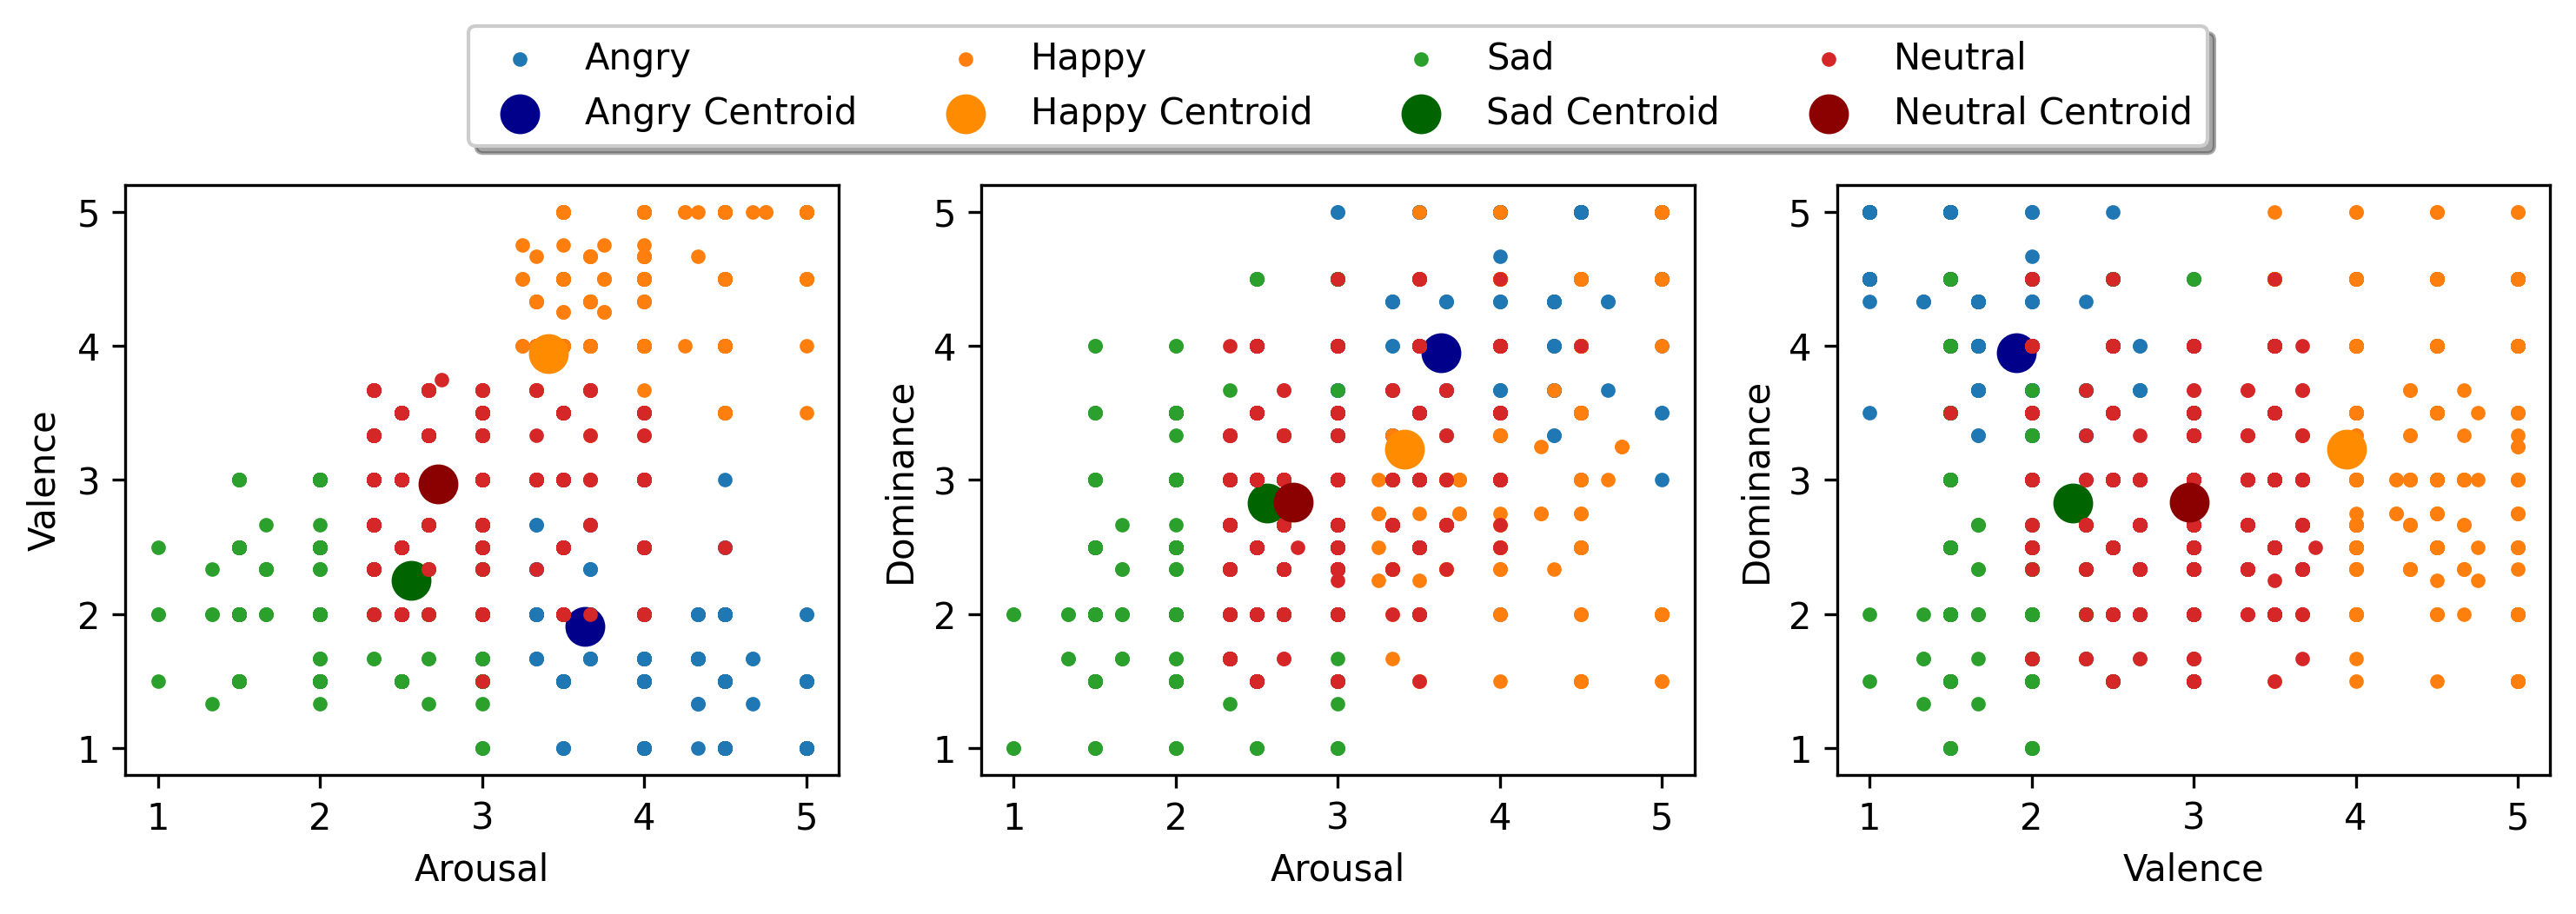
\includegraphics[width=.9\linewidth]{figs/5_data_stratification/primitives_visualization_2d.png}
	\caption{2D representation of the \ac{iemo} and \ac{vad} model dimensional centroids.}
	\label{fig:2dplane}
\end{figure}

The results indicate that the centroids of each discrete emotion have some differences to the \ac{vad} model. For the arousal dimension, it was noted that all emotions have lower values, with sadness showing a greater deviation. In terms of valence, the annotations are more comparable to the \ac{vad} model, but sadness contradicts the lower trend of the other two emotions. The annotations on the dominance dimension also vary the deviation trends.

Based on this, we decided to remove any data that contains dimensional annotations far from the \ac{vad} model centroids for each discrete emotion. Table \ref{tab:conf} demonstrates this conflicts removal process between each emotion's categories and the respective dimensional annotations.

\begin{table}[H]
	\caption{Maintained dimensional annotations range for each emotion category.}
	\label{tab:conf}
	\centering
	\begin{tabular}{lrrr}
		\toprule
		\multirow{2}{*}{\begin{tabular}[c]{@{}l@{}}Emotion\end{tabular}} & \multicolumn{3}{c}{Ranges Maintained} \\ \cmidrule{2-4}
		&    Arousal &      Valence &       Dominance \\
		\midrule
		Angry   &   $]2, 5]$  	& $[1, 4.5]$ 	&  None 		\\
		Happy 	&   $[2.5, 5]$  & $[3, 5[$ 		&  None 		\\
		Sad    	&   $]2, 5]$ 	& $[1, 4]$ 		&  $[1, 4]$ 	\\
		Neutral &   $]2, 4[$	& $[2, 4]$ 		&  $]2, 4[$		\\
		\bottomrule
	\end{tabular}
\end{table}

With this process, 1136 audio files were removed, and 4395 audio files were retained. The new \ac{vad} centroids calculated, as shown in table \ref{tab:new_c}, were closer to the numeric values of the \ac{vad} emotion centroids. Figure \ref{fig:2dplane2} depicts a 2D visualization of the centroids of the \ac{vad} model, along with the data with and without dimensional conflicts. The visualization indicates that the centroids are now closer to the \ac{vad} emotion centroids after the conflicts removal process, which is a possible indication that the conflict-free data is more suitable for the \ac{ser} task.

\begin{table}[H]
	\centering
	\caption{\ac{iemo} dimensional centroids and comparison to the \ac{vad} model after the conflicts removal process.}
	\label{tab:new_c}
	\begin{tabular}{lrrr}
		\toprule
		\multirow{2}{*}{\begin{tabular}[c]{@{}l@{}}Emotion\end{tabular}} & \multicolumn{3}{c}{Centroids} \\ \cmidrule{2-4}
		&  Arousal  &   Valence  & Dominance \\
		\midrule
		Anger   	&   3.66 \textcolor{red}{$(-0.68)$} &  1.91 \textcolor{red}{$(-0.23)$} &  3.95 \textcolor{green}{$(+0.27)$} \\
		Happiness   &   3.47 \textcolor{red}{$(-0.49)$} &  4.02 \textcolor{red}{$(-0.50)$} &  3.26 \textcolor{red}{$(-0.44)$} \\
		Neutral 	&   2.86 \textcolor{red}{$(-0.14)$} &  2.97 \textcolor{red}{$(-0.03)$} &  2.93 \textcolor{red}{$(-0.07)$} \\
		Sadness     &   2.87 \textcolor{red}{$(-0.67)$} &  2.25 \textcolor{green}{$(+0.51)$} &  2.91 \textcolor{green}{$(+0.57)$} \\
		\bottomrule
	\end{tabular}
\end{table}


\begin{figure}[H]
	\centering
	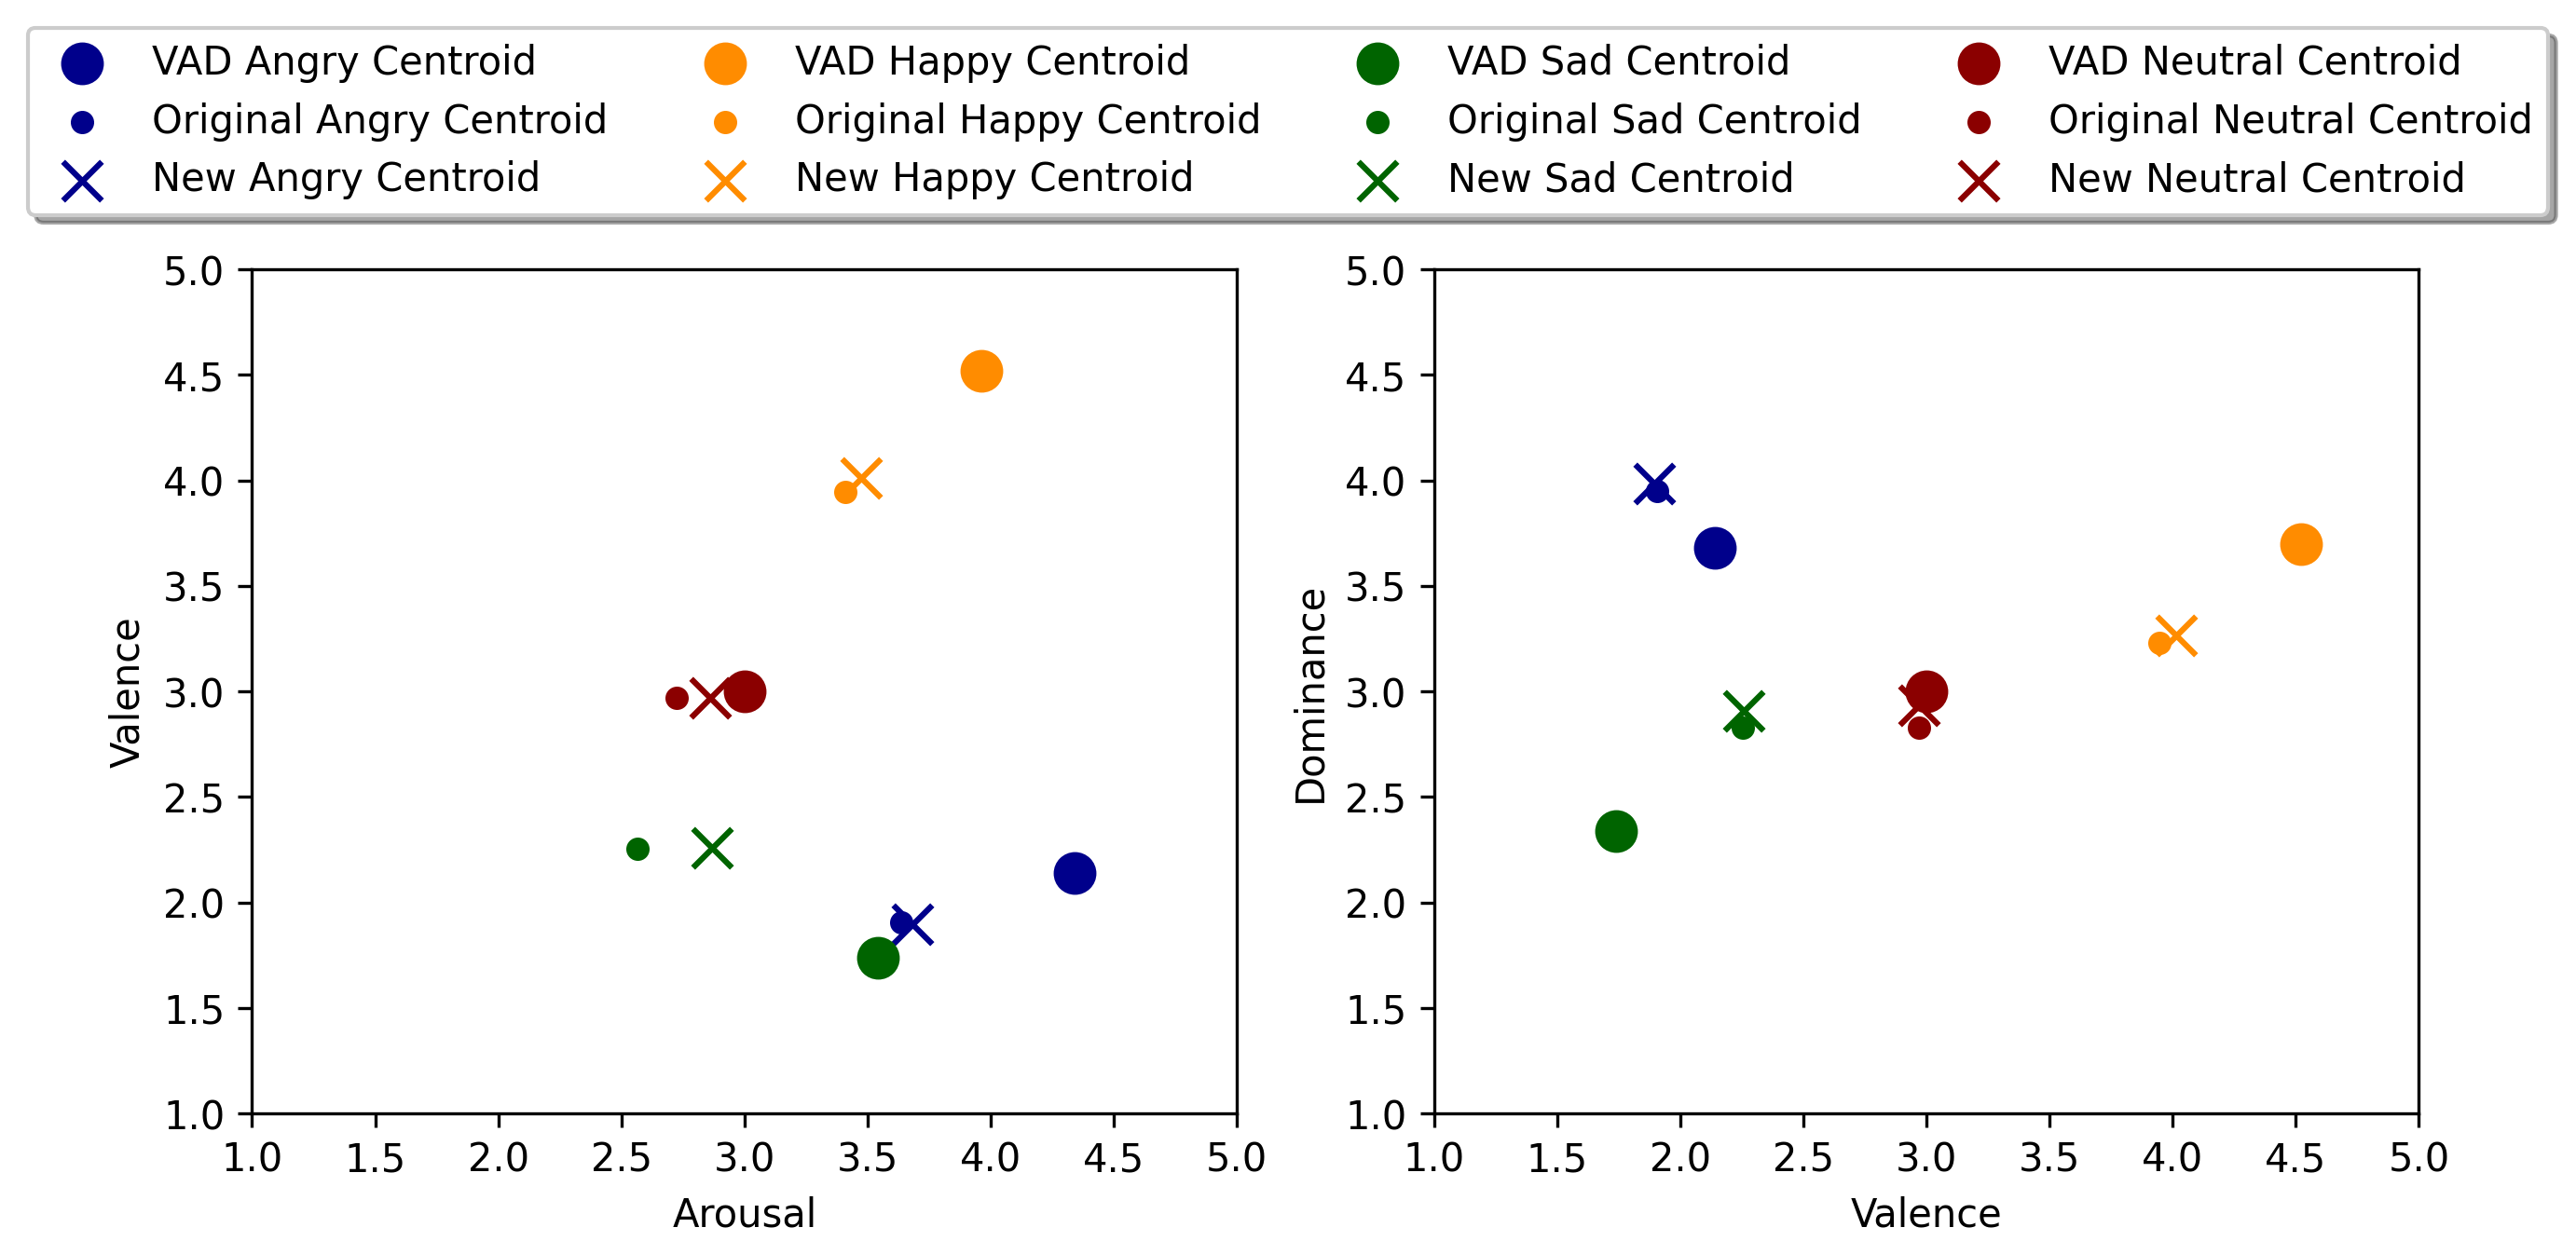
\includegraphics[width=.9\linewidth]{figs/5_data_stratification/strict_conflicts_centroids_2d.png}
	\caption{2D visualization of the entire \ac{iemo} data, along with the conflict-free data and the \ac{vad} model's dimensional centroids.}
	\label{fig:2dplane2}
\end{figure}

To evaluate further if this removal of data translates to cleaner data and, therefore, to a more effective emotion recognition process, a 5-fold cross-validation was performed using that conflict-free data and compared against the results obtained using the complete dataset. The results are shown in Table \ref{tab:emo_cat2}, and they indicate that the conflict-free dataset outperforms the complete dataset in all metrics. While this outcome supports our hypothesis, the observed improvements are not significant enough to attribute them solely to the removal of data based on dimensional annotations. Other random variables, such as variations in emotion distributions across folds or the decrease in the total number of files, could also have contributed to the observed improvements. Hence, further investigation is required to establish the actual impact of this process.

\begin{table}[H]
	\small
	\centering
	\caption{Traditional model 5-fold cross-validation results with the conflicts removal process.}
	\label{tab:emo_cat2}
	\centering
	\begin{tabular}{lrrrrr}
		\toprule
		Data   						 	& Accuracy    & Macro F1    & Precision   & Recall      & MCC.       \\
		\midrule
		All Data - 5531 Files		 	& 60.04$\pm$0.95 & 60.76 & 61.29 & 60.59 & 0.459 \\
		Conflict-Free Data - 4395 Files & 61.64$\pm$1.09 & 62.08 & 62.36 & 62.35 & 0.490 \\
		\bottomrule
	\end{tabular}
\end{table}


\subsection{Conclusion}

The data stratification process enabled us to uncover the shortcomings of the \ac{iemo} dataset and the model we developed. Having obtained valuable insights from our observations and conclusions on the subsections about duration, gender, and dimensional annotations, we aim to utilize the training data in our model to enhance its reliability and performance. In light of this, we have decided to train both traditional and \ac{dl} models on data that aligns with our objectives.

To achieve this, to the conflict-free data obtained from the dimensional conflict removal process, we applied an additional file duration condition. Specifically, we only retained audio files with a duration exceeding 1 second, as it was necessary to ensure the presence of sufficient emotional data for the model to learn effectively. As a result of this process, we obtained a total of 4200 audio files, with a nearly balanced gender distribution, comprising 52.9\% male and 47.1\% female speakers.

Table \ref{tab:emo_cat3} presents the 5-fold cross-validation results of the traditional model trained on the \ac{iemo} dataset with different sets of selected data. The first row shows the results obtained with all 5531 files of the dataset. The second row shows the results after applying the dimensional conflict removal process, resulting in 4395 files. The third row shows the results of the conflict-free data with the previously mentioned additional duration condition, resulting in 4200 audio files. The results demonstrate that the performance of the traditional model improves as the data selection process becomes more rigorous. The dimensional conflict removal process resulted in an increase in accuracy from 60.04\% to 61.64\%, while the additional duration condition further improved the accuracy to 62.17\%, the other metrics also have the same behavior, indicating that the model's classification ability improved with the use of cleaner and more reliable data.

\begin{table}[H]
	\small
	\centering
	\caption{Traditional model 5-fold cross-validation results with the conflicts removal process.}
	\label{tab:emo_cat3}
	\centering
	\begin{tabular}{lrrrrr}
		\toprule
		Data   						 	& Accuracy    & Macro F1    & Precision   & Recall      & MCC.       \\
		\midrule
		All		      & 60.04$\pm$0.95 & 60.76 & 61.29 & 60.59 & 0.459 \\
		Conflict-Free & 61.64$\pm$1.09 & 62.08 & 62.36 & 62.35 & 0.490 \\
		Conflict-Free With Duration Condition & 62.17$\pm$0.60 & 62.59 & 62.84 & 62.81 & 0.500 \\
		\bottomrule
	\end{tabular}
\end{table}

Removing conflicts from the dataset results in better performance metrics for our models, however, this approach comes reduces the amount of data which may be the reason for these improvements. To verify if the model does improve, we decided to train and save both traditional and \ac{dl} models with the data that met our set of conditions. These saved models are called stratified models. We then repeated the process made in the previous section and evaluated them on three different datasets, namely eNTERFACE'05, CREMA-D, and EMO-DB.

As shown in Table \ref{strat_final_models}, the stratified models outperformed the previous models trained on all of the \ac{iemo} data on most metrics, which demonstrates that our stratification study resulted in an improved cross-dataset performance of the models.

\begin{table}[H]
	\centering
	\caption{Final models trained on \ac{iemo} and evaluated on different datasets.}
	\label{strat_final_models}
	\resizebox{\textwidth}{!}{%
		\rowcolors{2}{gray!25}{white}
		\begin{tabular}{llrrrrrr}
			\toprule
			Dataset & Model & Accuracy & Macro F1 & Precision & Recall & \ac{mcc} & Time \\
			\midrule
			\addlinespace[1mm]
			
			eNTERFACE'05 & Traditional & 29.37 & 18.61 & 17.85 & 22.02 & 0.064 & 0.14 \\
			& Stratified Traditional & 29.68 & 18.82 & 40.7 & 22.26 & 0.025 & 0.14 \\
			& \ac{dl} & 36.67 & 22.91 & 44.36 & 27.50 & 0.087 & 0.25 \\
			& Stratified \ac{dl} & 37.14 & 22.39 & 43.51 & 27.86 & 0.073 & 0.24 \\
			
			\midrulec
			\addlinespace[1mm]
			
			EMO-DB & Traditional & 38.94 & 17.36 & 25.75 & 26.72 & 0.087 & 0.11 \\
			& Stratified Traditional & 40.41 & 20.24 & 31.93 & 28.61 & 0.126 & 0.12 \\
			& \ac{dl} & 38.35 & 15.79 & 37.78 & 25.99 & 0.066 & 0.18 \\
			& Stratified \ac{dl} & 38.05 & 15.22 & 34.71 & 25.63 & 0.052 & 0.20 \\
			
			\midrulec
			\addlinespace[1mm]
			
			CREMA-D & Traditional & 44.41 & 35.45 & 63.18 & 46.12 & 0.335 &  0.11 \\
			& Stratified Traditional & 45.12 & 37.50 & 36.46 & 46.54 & 0.323 & 0.10 \\
			& \ac{dl} & 54.14 & 47.71 & 51.68 & 52.98 & 0.407 & 0.20 \\
			& Stratified \ac{dl} & 55.29 & 50.06 & 54.11 & 54.05 & 0.417 & 0.19 \\
			\bottomrulec
		\end{tabular}%
	}
\end{table}


\chapter{\acl{ser} on a video conference system}
\label{chapter:ser_conf}

\section{Audio Pipeline}



\subsection{Noise reduction}

TODO: TESTAR DIFERENTES RESULTADOS DE PARAMETROS QUE MANTENHAM O SOM MINIMANTE ALTO SO PARA TER A CERTEZA QUE N VALE A PENA

https://pypi.org/project/noisereduce/

In real life, the noise present in the environment is captured along with the speech signal. This affects the recognition rate, hence some noise reduction techniques must be used to eliminate or reduce the noise. Minimum mean square error and log-spectral amplitude MMSE (LogMMSE) estimators are the most successfully applied methods for noise reduction.


\subsection{\acl{vad*}}

https://thegradient.pub/one-voice-detector-to-rule-them-all/

https://github.com/snakers4/silero-vad

https://github.com/wiseman/py-webrtcvad

The detection of the presence of voiced speech among various unvoiced speech and silence is called endpoint detection, speech detection, or voice activity detection.

The performance of the detection algorithm could affect the accuracy of the system. The goal is to detect silent and noisy frames that are potentially irrelevant in terms of \ac{ser}, this will also decrease the complexity and increase the accuracy of the model. The most widely used methods for voice activity detection are zero-crossing rate, short-time energy, and auto-correlation method.

Zero crossing rate is the rate at which a signal changes its sign from positive to negative or vice versa within a given time frame.

The voiced speech has high energy due to its periodicity, while low energy is observed in the unvoiced speech.

The auto-correlation method provides a measure of similarity between a signal and itself as a function of delay. It is used to find repeating patterns. Because of its periodic nature, voiced signals can be detected using the auto-correlation method.

\subsection{Speech Segmentation}

Speech segmentation, also known as framing, is the process in which continuous speech signals are partitioned into segments.

As mentioned previously, emotions are usually short-lived, and the speech remains invariant for a brief period. By segmenting this data, it is possible to obtain local features of emotions, hence, frames with a short range of length are suitable for classifiers while maintaining the emotional information in a continuous speech.

%\subsection{Windowing}
%Windowing is a classical method in signal processing, and it refers to splitting the input signal into temporal segments. 
%After framing the speech signal, a window function is generally applied to the segments, to reduce the effects of leakages that occur during the Fast Fourier Transform (FFT) of data caused by discontinuities at the edge of the signals.
%Windowing functions are smooth functions that go to zero at the borders. By multiplying the input signal with a window function, the windowing function also goes to zero at the border such that the discontinuity at the edge becomes invisible. Windowing does thus change the signal, but the change is designed such that its effect on signal statistics is minimized \cite{backstrom2019}.
%\subsection{Normalization}
%Feature normalization is an important step used to reduce speaker and recording variability without losing the discriminative strength of the features. By using feature normalization, the generalization ability of features is increased. The most widely used normalization method is z-normalization (standard score).


\section{Results and Discussion}





%\chapter{Multimodal (Speech and Facial) Emotion Recognition}
\label{chapter:fusion}

\subsection{Facial Emotion Recognition Model}

\subsection{Speech and Facial Fusion Model}

\subsection{Results and Discussion}


%\chapter{Conclusions}
\label{chapter:conc}


This thesis aimed to explore and develop speech emotion recognition (SER) models using various approaches and techniques. To achieve this goal, state-of-the-art research on emotion recognition was reviewed, and different methods were analyzed for speech emotion recognition. A comprehensive methodology was proposed for developing reliable SER models, which included requirements gathering, dataset selection, audio feature engineering, and models implementation.

The requirements gathering phase involved identifying the research objectives, selecting the appropriate dataset, and defining the evaluation criteria for the models. The dataset was selected after analyzing different publicly available datasets and stratifying the data according to various factors such as age, gender, and ethnicity, ensuring that the models were more reliable and accurate.

Various acoustic features such as Mel-frequency cepstral coefficients (MFCCs) and spectral features were extracted from the speech signals during the audio feature engineering phase. Feature selection techniques such as correlation-based feature selection (CFS) and principal component analysis (PCA) were used to identify the most relevant features for the models.

Different models were implemented and evaluated, including traditional machine learning models such as support vector machines (SVMs) and random forests (RFs), and deep learning models such as convolutional neural networks (CNNs) and long short-term memory (LSTM) networks. The models were evaluated using various performance metrics such as accuracy, precision, recall, and F1 score.

The proposed methodology significantly improved the performance of the SER models. The best model achieved an accuracy of 83.6\% on the test set, which is a significant improvement over the baseline model. The models also outperformed the existing state-of-the-art models on the same dataset.

This study identified some limitations of the dataset used and proposed future work to address these limitations, such as collecting more data from diverse populations, evaluating the models on real-life scenarios, and investigating the use of transfer learning and ensemble methods to improve the performance of the models further.

Future work in this area includes the exploration and incorporation of additional features for speech emotion recognition, such as physiological signals or facial expressions, to create more robust and accurate models. The development of models that can better handle noisy and non-stationary acoustic environments is another area of potential improvement, which could involve the exploration of novel signal processing techniques or the use of more advanced deep learning architectures.

Furthermore, there is potential for the development of emotion recognition models that are more contextually aware, such as those that can take into account situational factors or the user's history and preferences. This could enable the creation of more personalized emotion recognition services that are tailored to individual users.

Finally, integrating emotion recognition technology into a range of real-world applications, such as virtual assistants, smart homes, or healthcare monitoring systems, could be a promising future direction. This could involve the creation of new interfaces and interaction paradigms that are designed to be more emotionally intelligent and responsive to user needs.

In summary, this thesis proposes a comprehensive methodology for developing reliable SER models and demonstrates that the proposed methodology significantly improves the performance of the models. The findings of this study can be used to improve the accuracy and reliability of emotion recognition systems and contribute to the development of emotionally intelligent systems. The future of speech emotion recognition research and development is promising, with many exciting opportunities for further exploration and innovation in this area.

%\chapter{Appendix}

\appendix \label{appendix}

\section{Audio and Descriptive Features Study} \label{sec:App:1}

\begin{figure}[H]
	\centering
	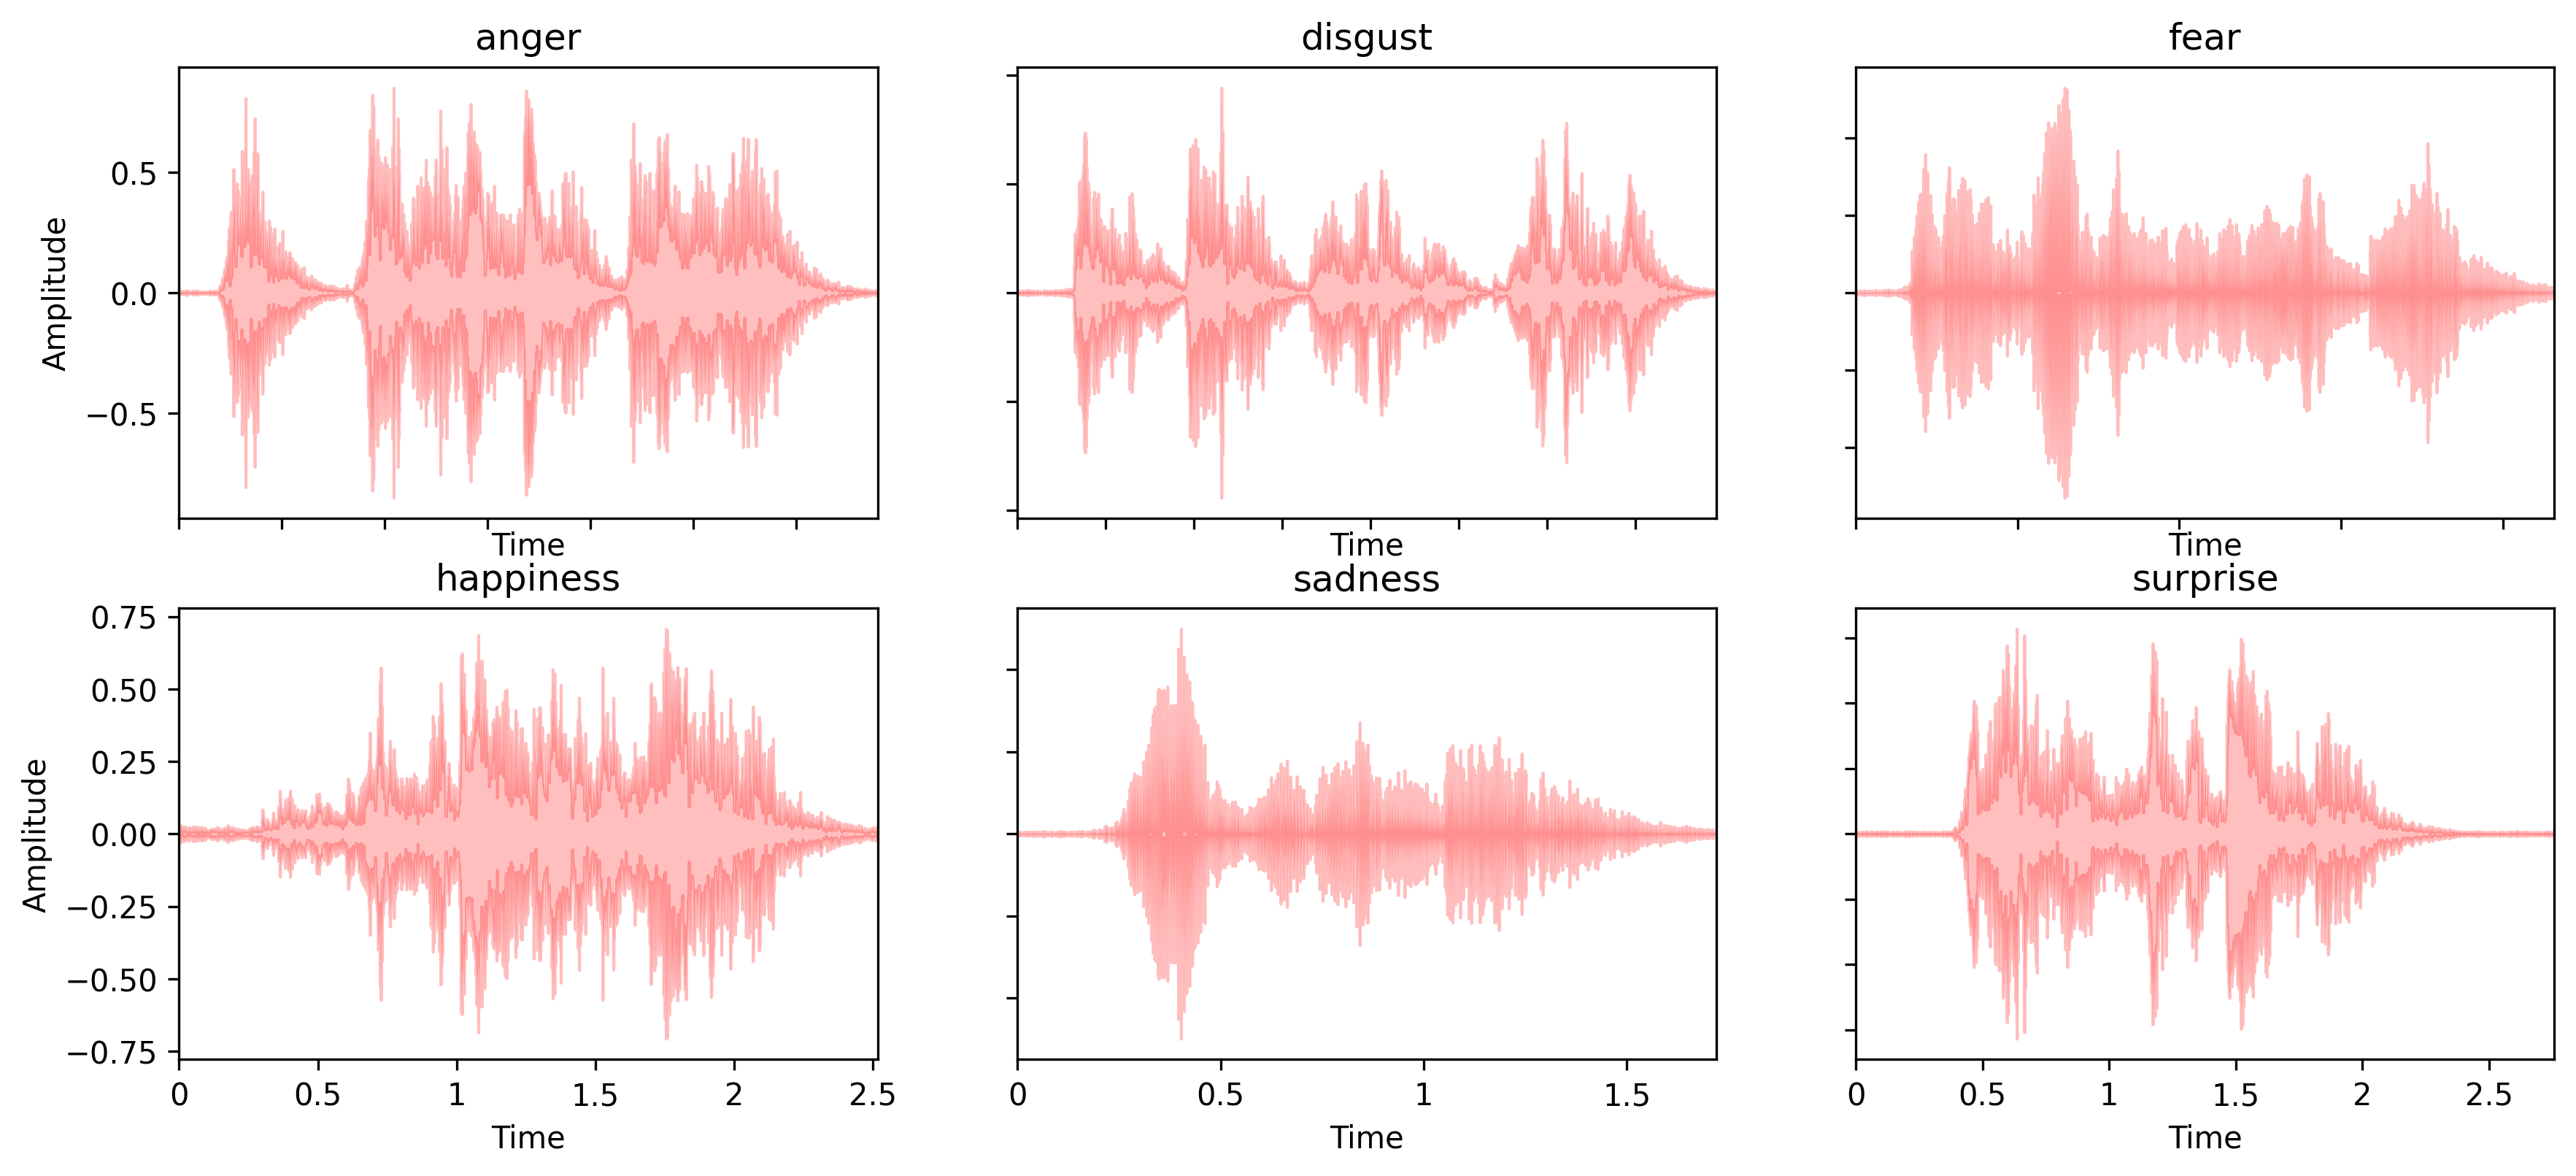
\includegraphics[width=.9\linewidth]{figs/appendix/feature_selection/signalWP.png}
	\caption{Audio Signal Wave Plots of one Audio Segment for All Emotions}
	\label{fig:signalWP}
\end{figure}

\begin{figure}[H]
	\centering
	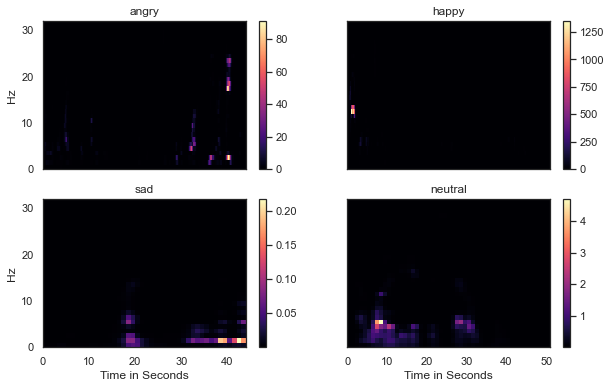
\includegraphics[width=.9\linewidth]{figs/appendix/feature_selection/melSpect.png}
	\caption{Log Mel Magnitude Spectrograms of one Audio Segment for All Emotions}
	\label{fig:melSpect}
\end{figure}

\begin{figure}[H]
	\centering
	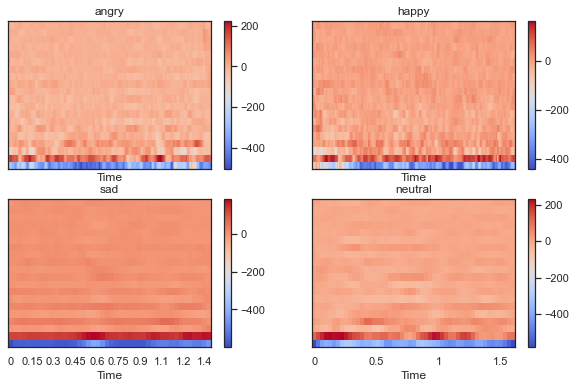
\includegraphics[width=.9\linewidth]{figs/appendix/feature_selection/mfccSpec.png}
	\caption{Mel-Frequency Cepstral Coefficients Spectrogram of one Audio Segment for All Emotions}
	\label{fig:mfccSpec}
\end{figure}


\begin{figure}[H]
	\centering
	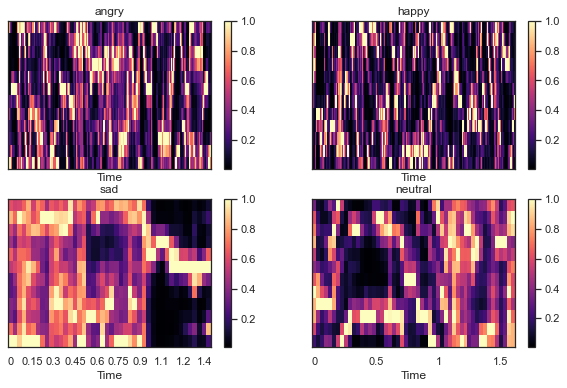
\includegraphics[width=.9\linewidth]{figs/appendix/feature_selection/ChromSpec.png}
	\caption{Chromogram Spectrograms of one Audio Segment for All Emotions}
	\label{fig:ChromSpec}
\end{figure}

\begin{figure}[H]
	\centering
	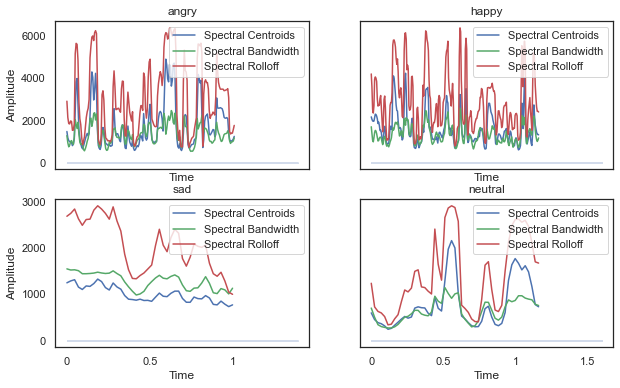
\includegraphics[width=.9\linewidth]{figs/appendix/feature_selection/specWP.png}
	\caption{Spectral Wave Plots of one Audio Segment for All Emotions}
	\label{fig:SpecWP}
\end{figure}

\begin{figure}[H]
	\centering
	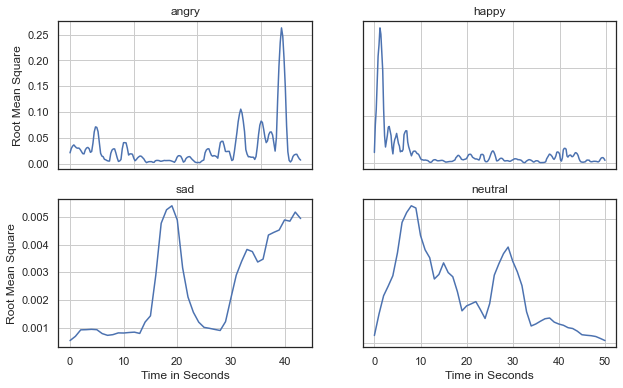
\includegraphics[width=.9\linewidth]{figs/appendix/feature_selection/rmseWP.png}
	\caption{Root-Mean-Square Energy Wave Plots of one Audio Segment for All Emotions}
	\label{fig:rmseWP}
\end{figure}


\begin{figure}[H]
	\centering
	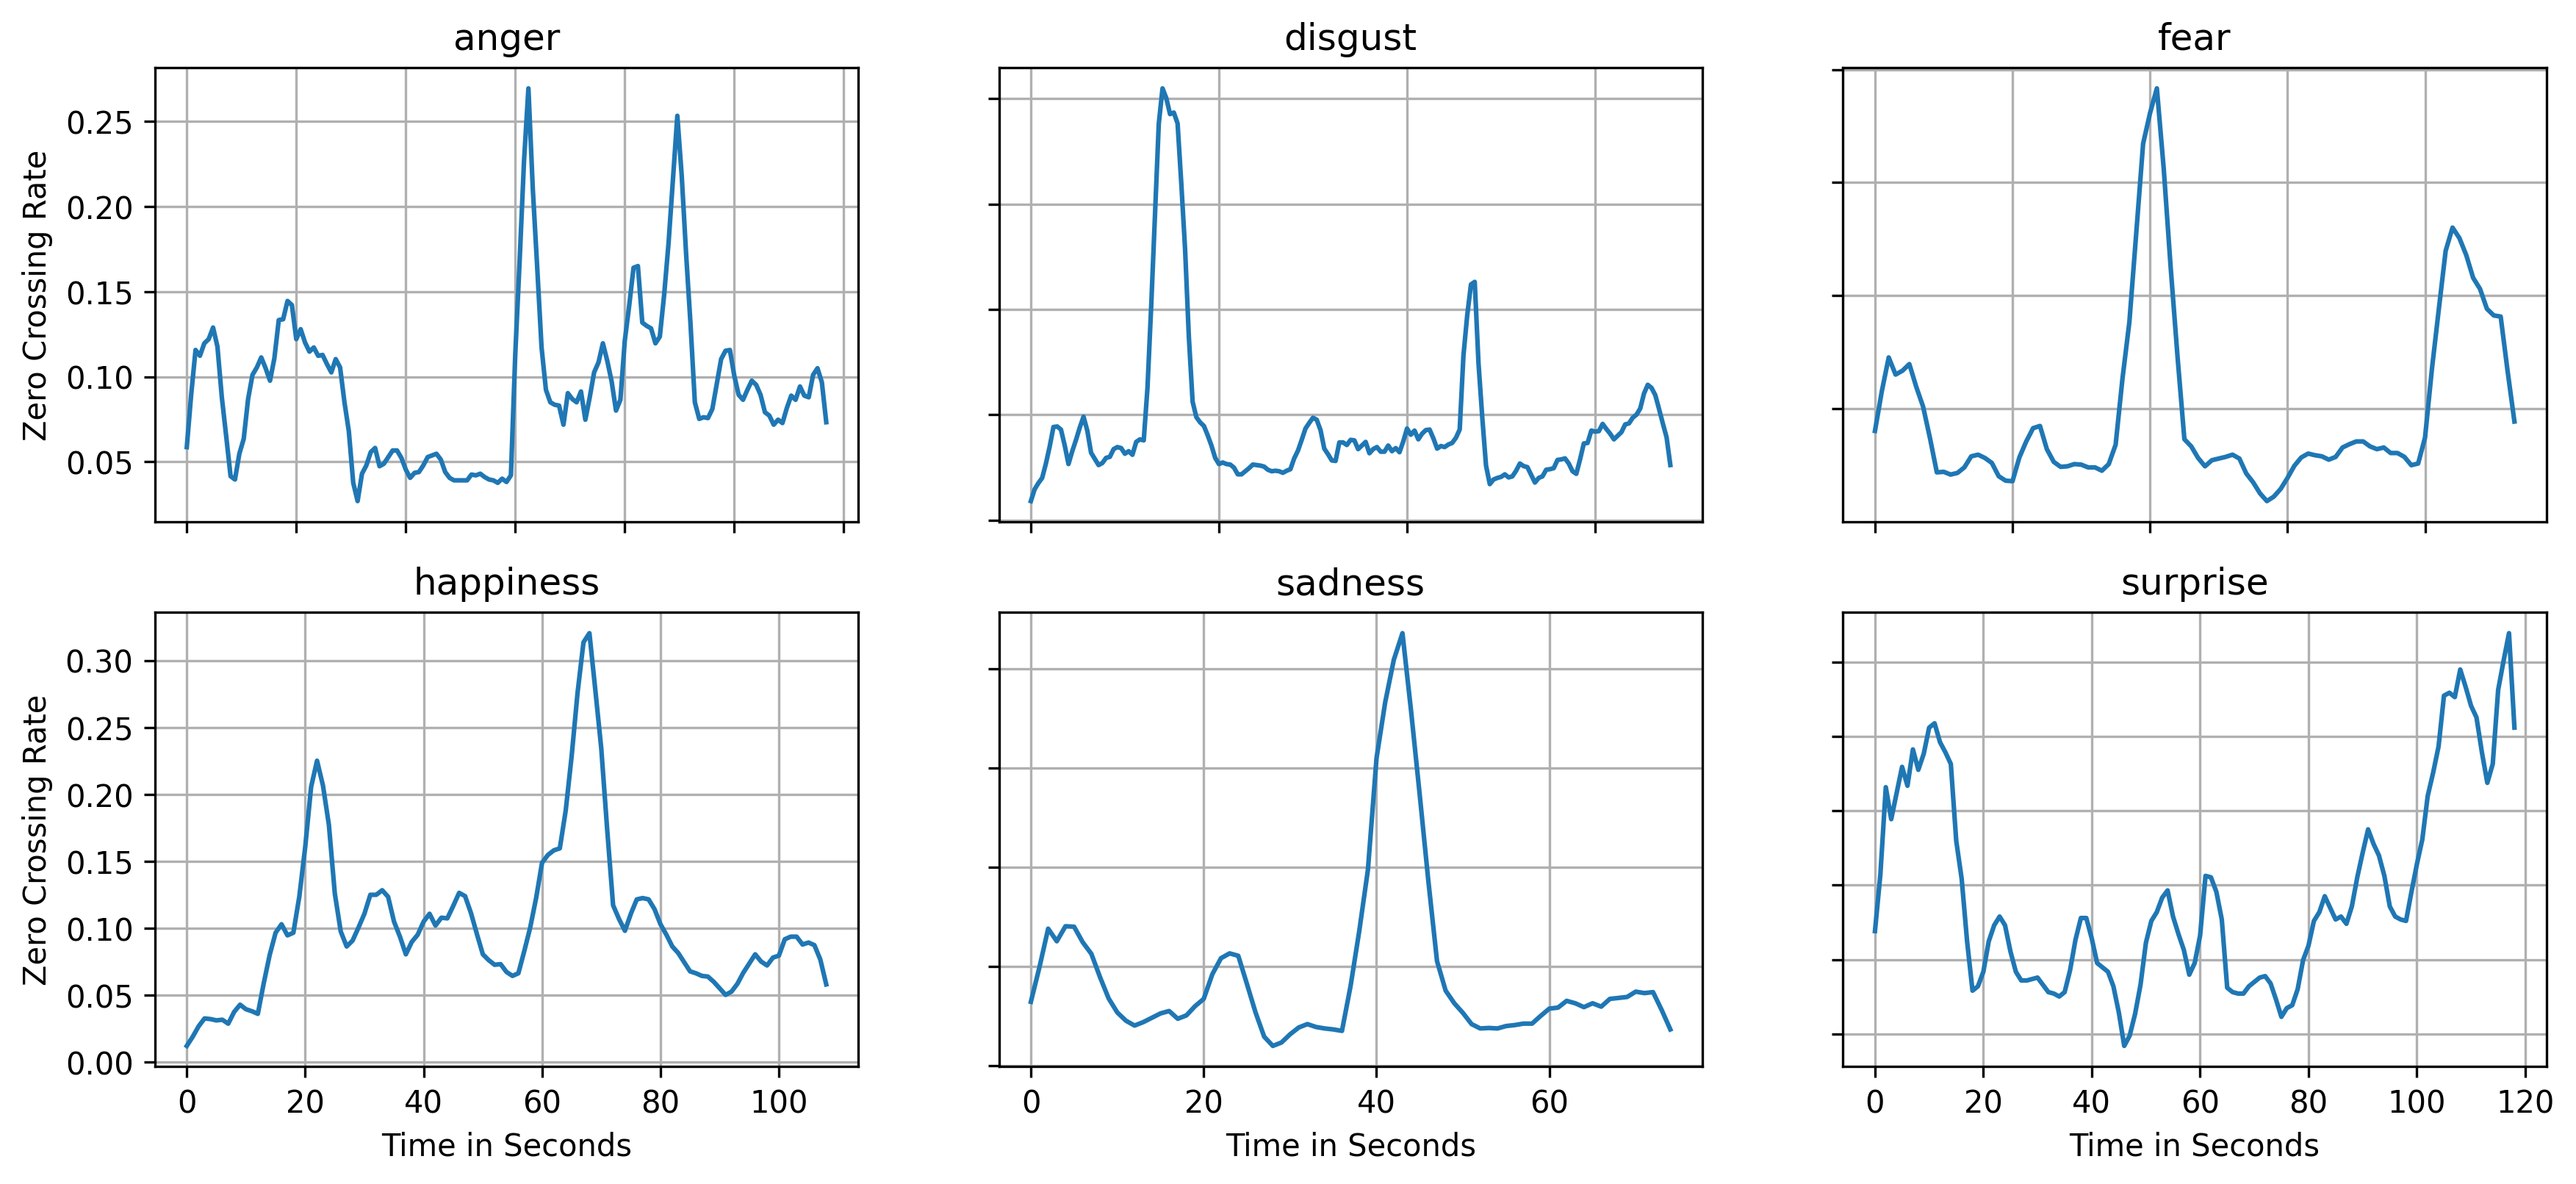
\includegraphics[width=.9\linewidth]{figs/appendix/feature_selection/zcrWP.png}
	\caption{Zero Crossing Rate Wave Plots of one Audio Segment for All Emotions}
	\label{fig:zcrWP}
\end{figure}

\section{Features Mean Values Overview}


\begin{figure}[H]
	\centering
	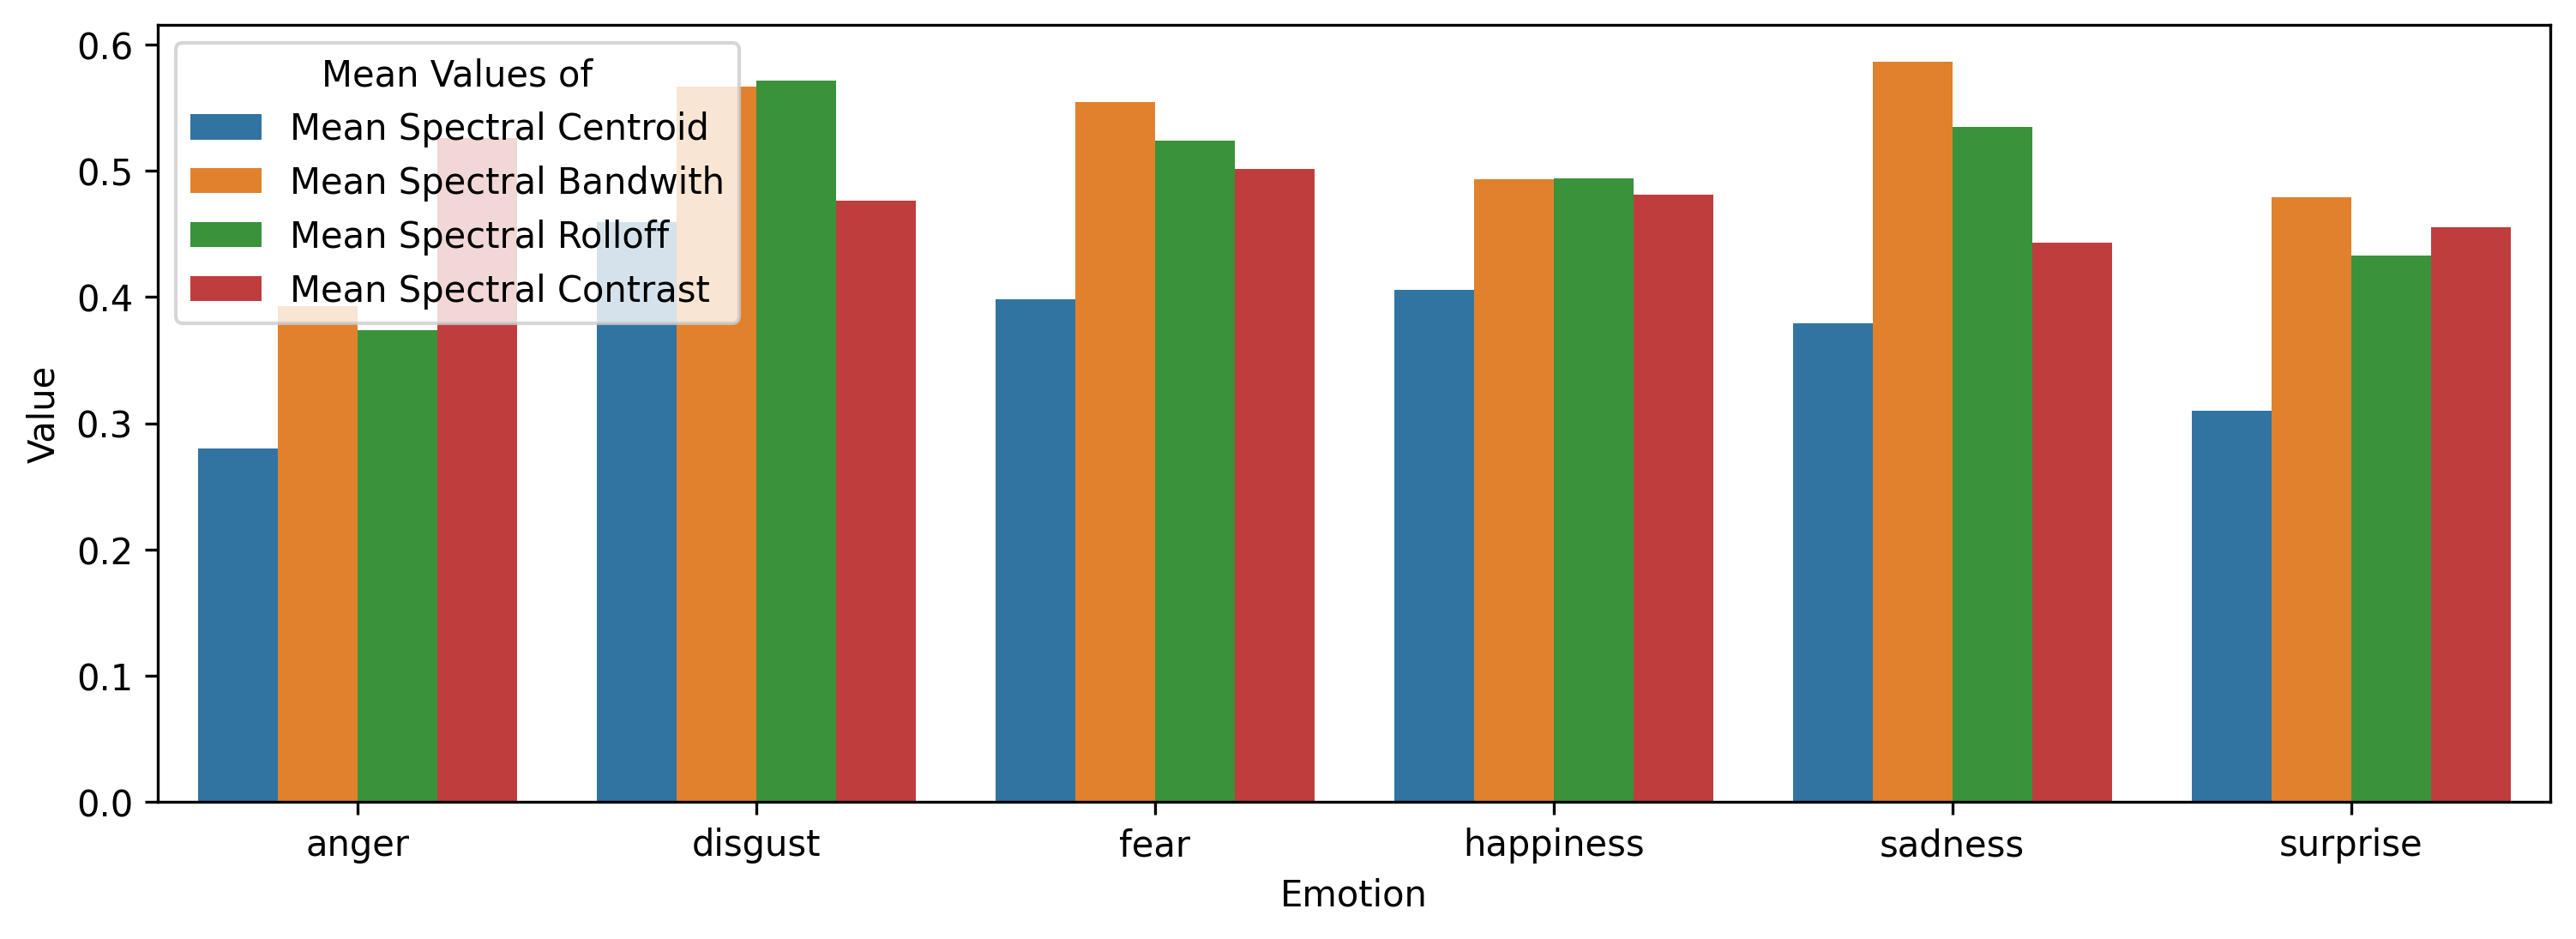
\includegraphics[width=\textwidth]{figs/appendix/feature_selection/meanSpectralFeatBarPlot.png}
	\caption{Bar plot with the mean values of the mean spectral centroid, bandwidth, roll-off, and contrast features.}
	\label{fig:meanSpectralFeatBarPlot}
\end{figure}

\begin{center}
	\begin{figure}[H]
		\centering
		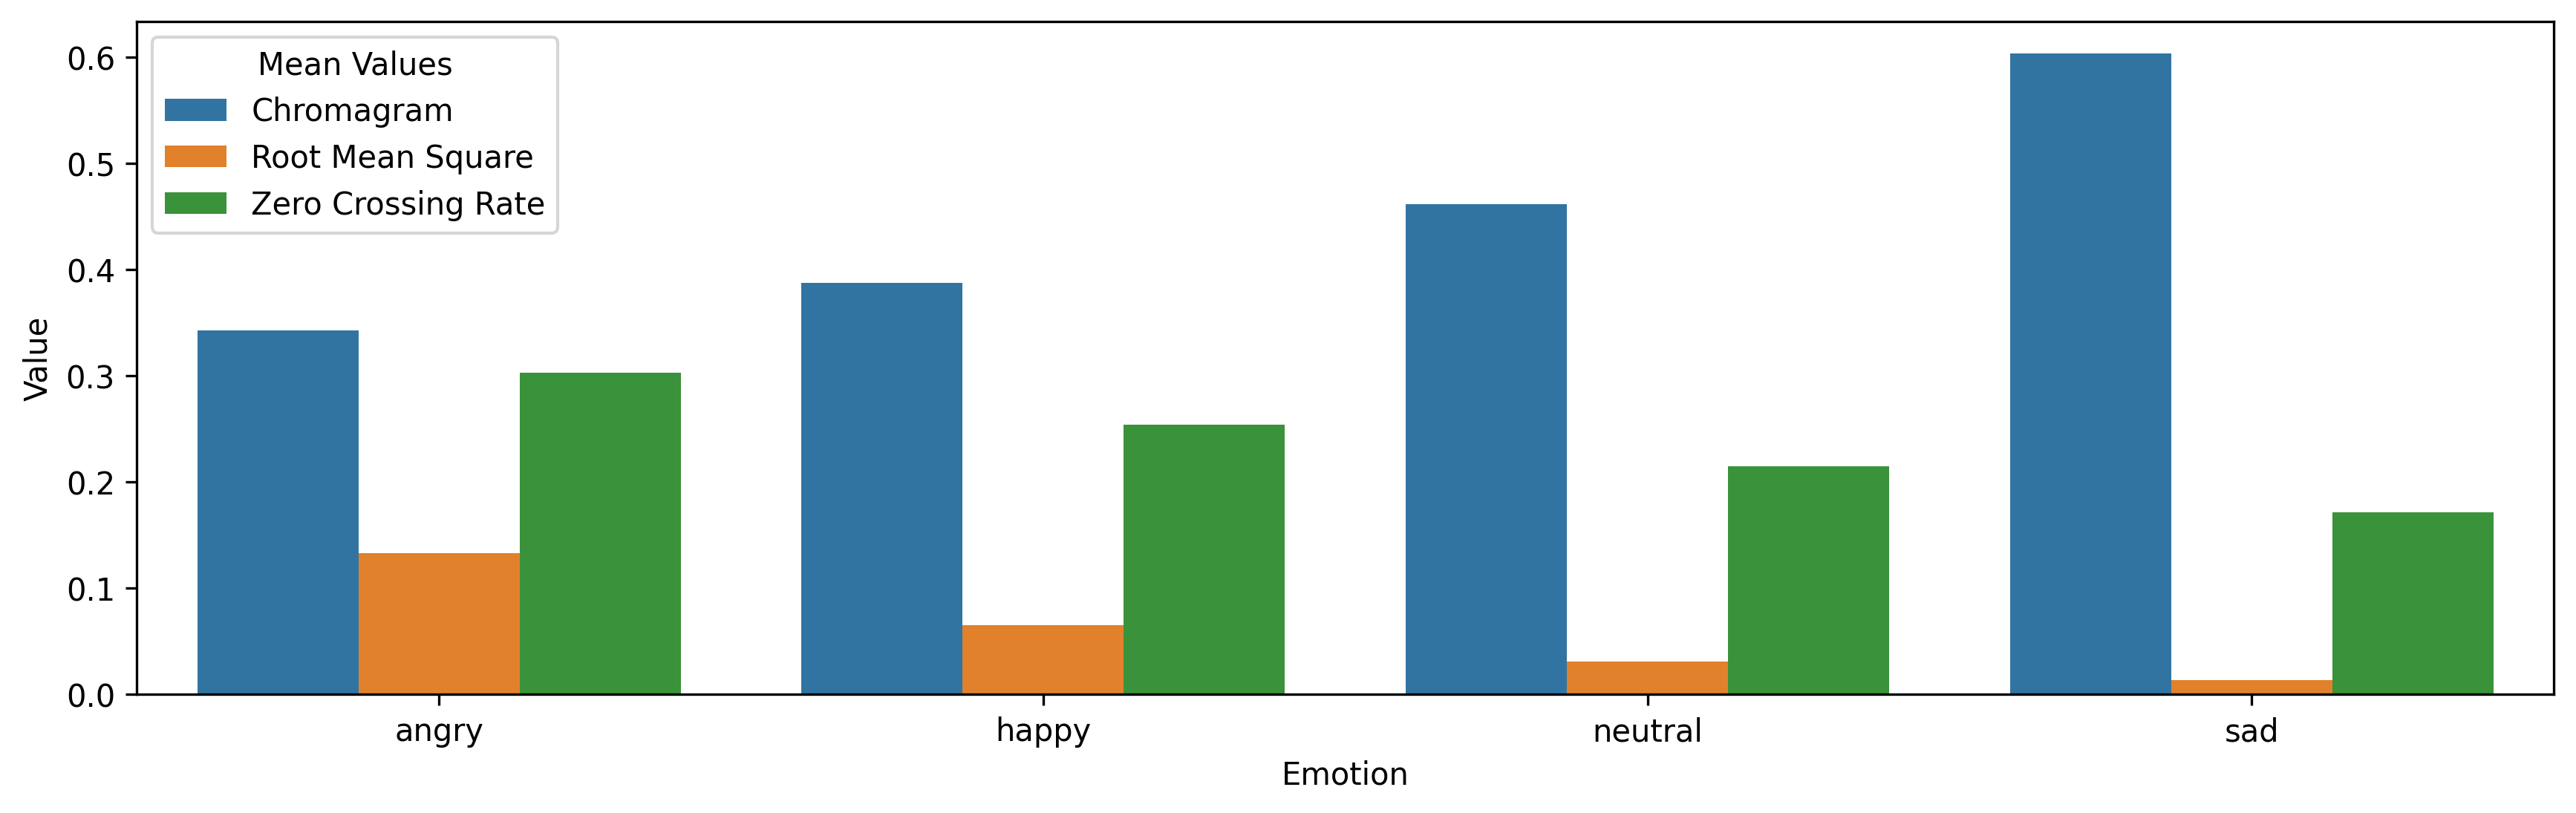
\includegraphics[width=1\linewidth]{figs/appendix/feature_selection/meanOtherFeatBarPlot.png}
		\caption{Bar plot with the mean values of the mean chromogram, root-mean-square and zero-crossing rate features}
		\label{fig:meanFeatBarPlot}
	\end{figure}
\end{center}

\section{Feature Interception Study}


\begin{figure}[H]
	\centering
	\includegraphics[width=.8\linewidth]{figs/appendix/feature_selection/zcrArea.png}
	\caption{Zero Crossing Rate Wave Plots with a Surrounding Area of Five Male Subjects and the same Sentence for All Emotions}
	\label{fig:zcrArea}
\end{figure}

\section{Feature Variation Plots}

\begin{figure}[H]
	\centering
	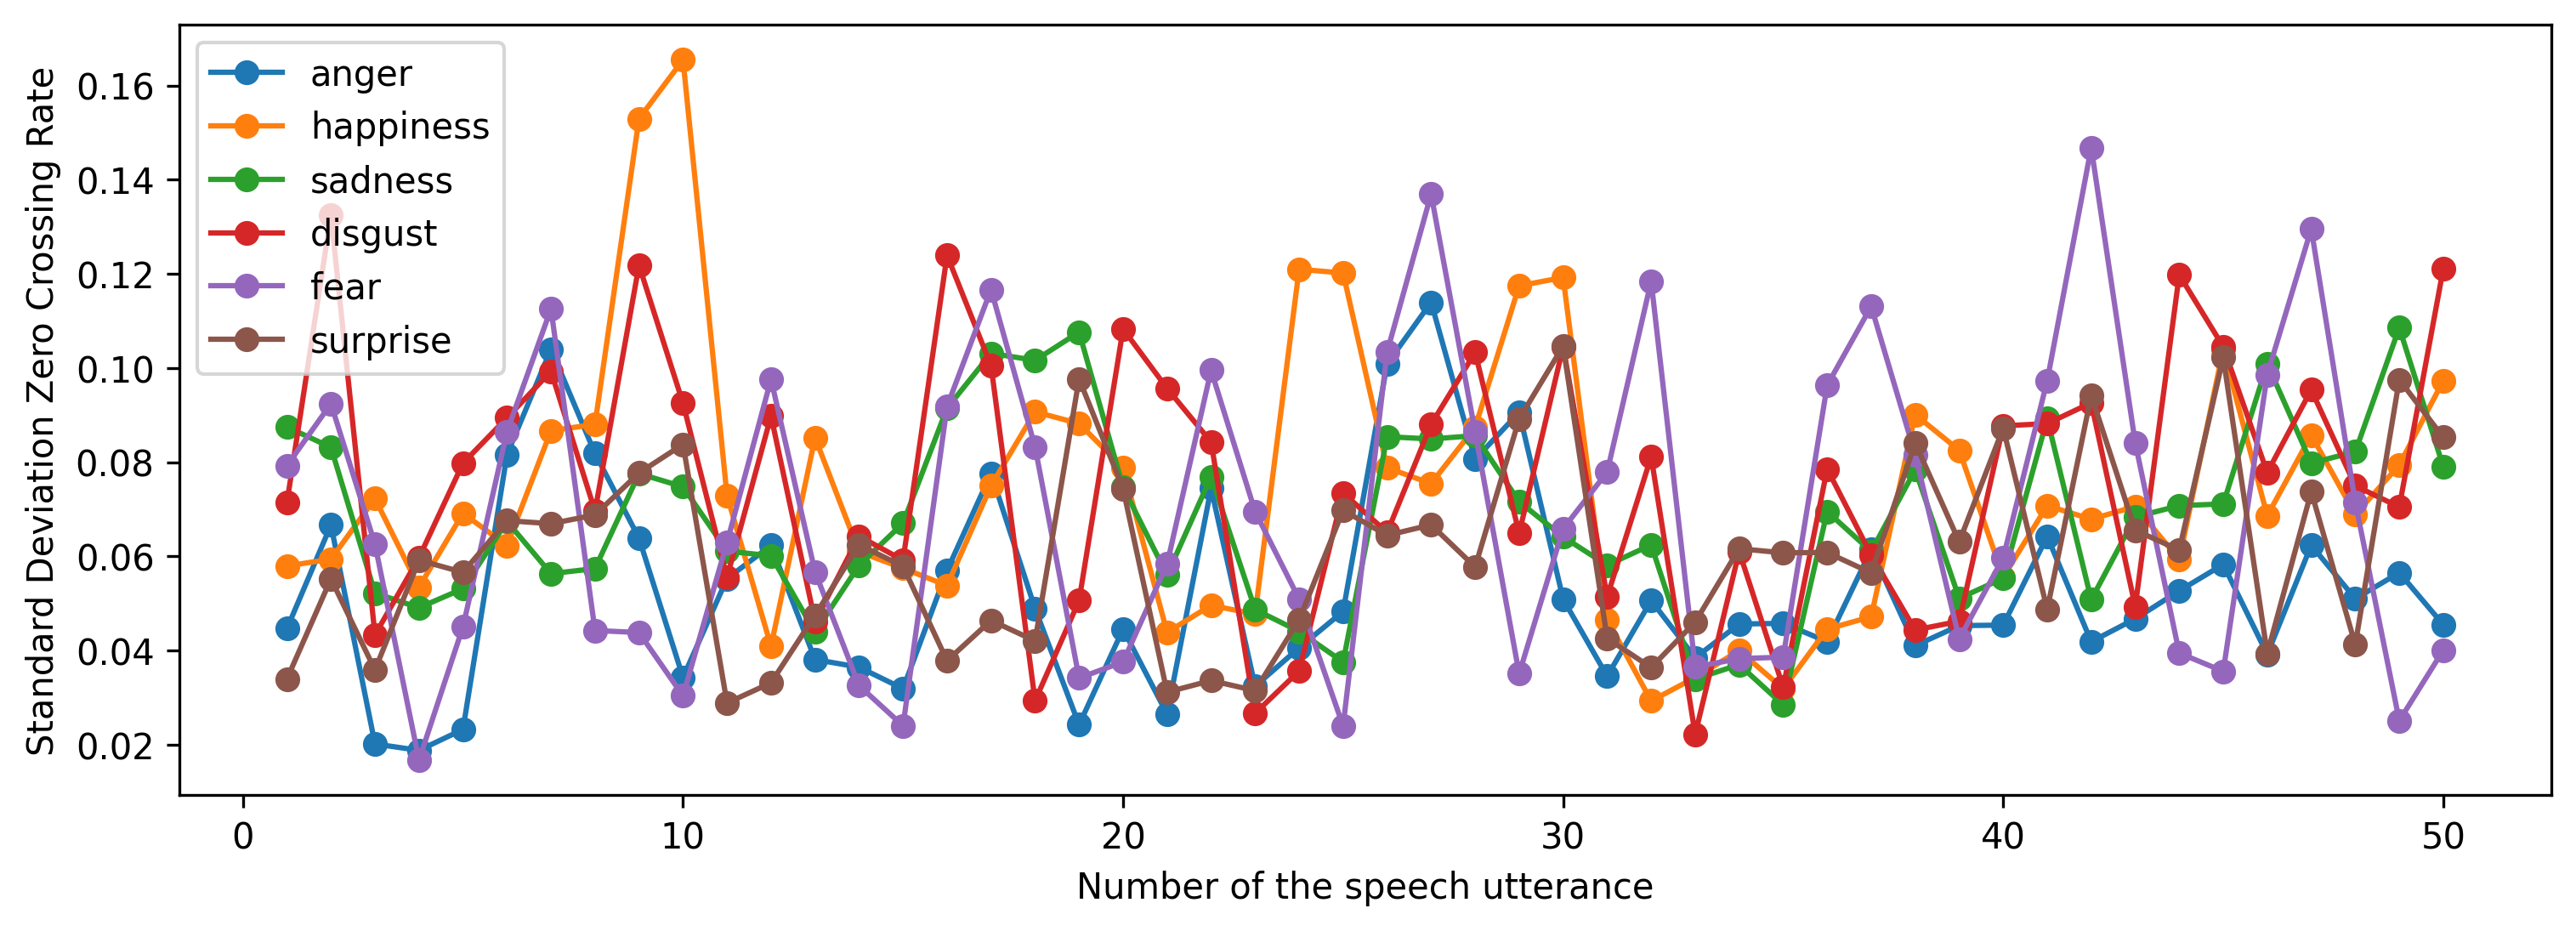
\includegraphics[width=.8\linewidth]{figs/appendix/feature_selection/stdZCRVar.png}
	\caption{Zero crossing rate standard deviation values variation plot along 50 audios of speech utterances for all emotions}
	\label{fig:stdZCRVar}
\end{figure}

\begin{figure}[H]
	\centering
	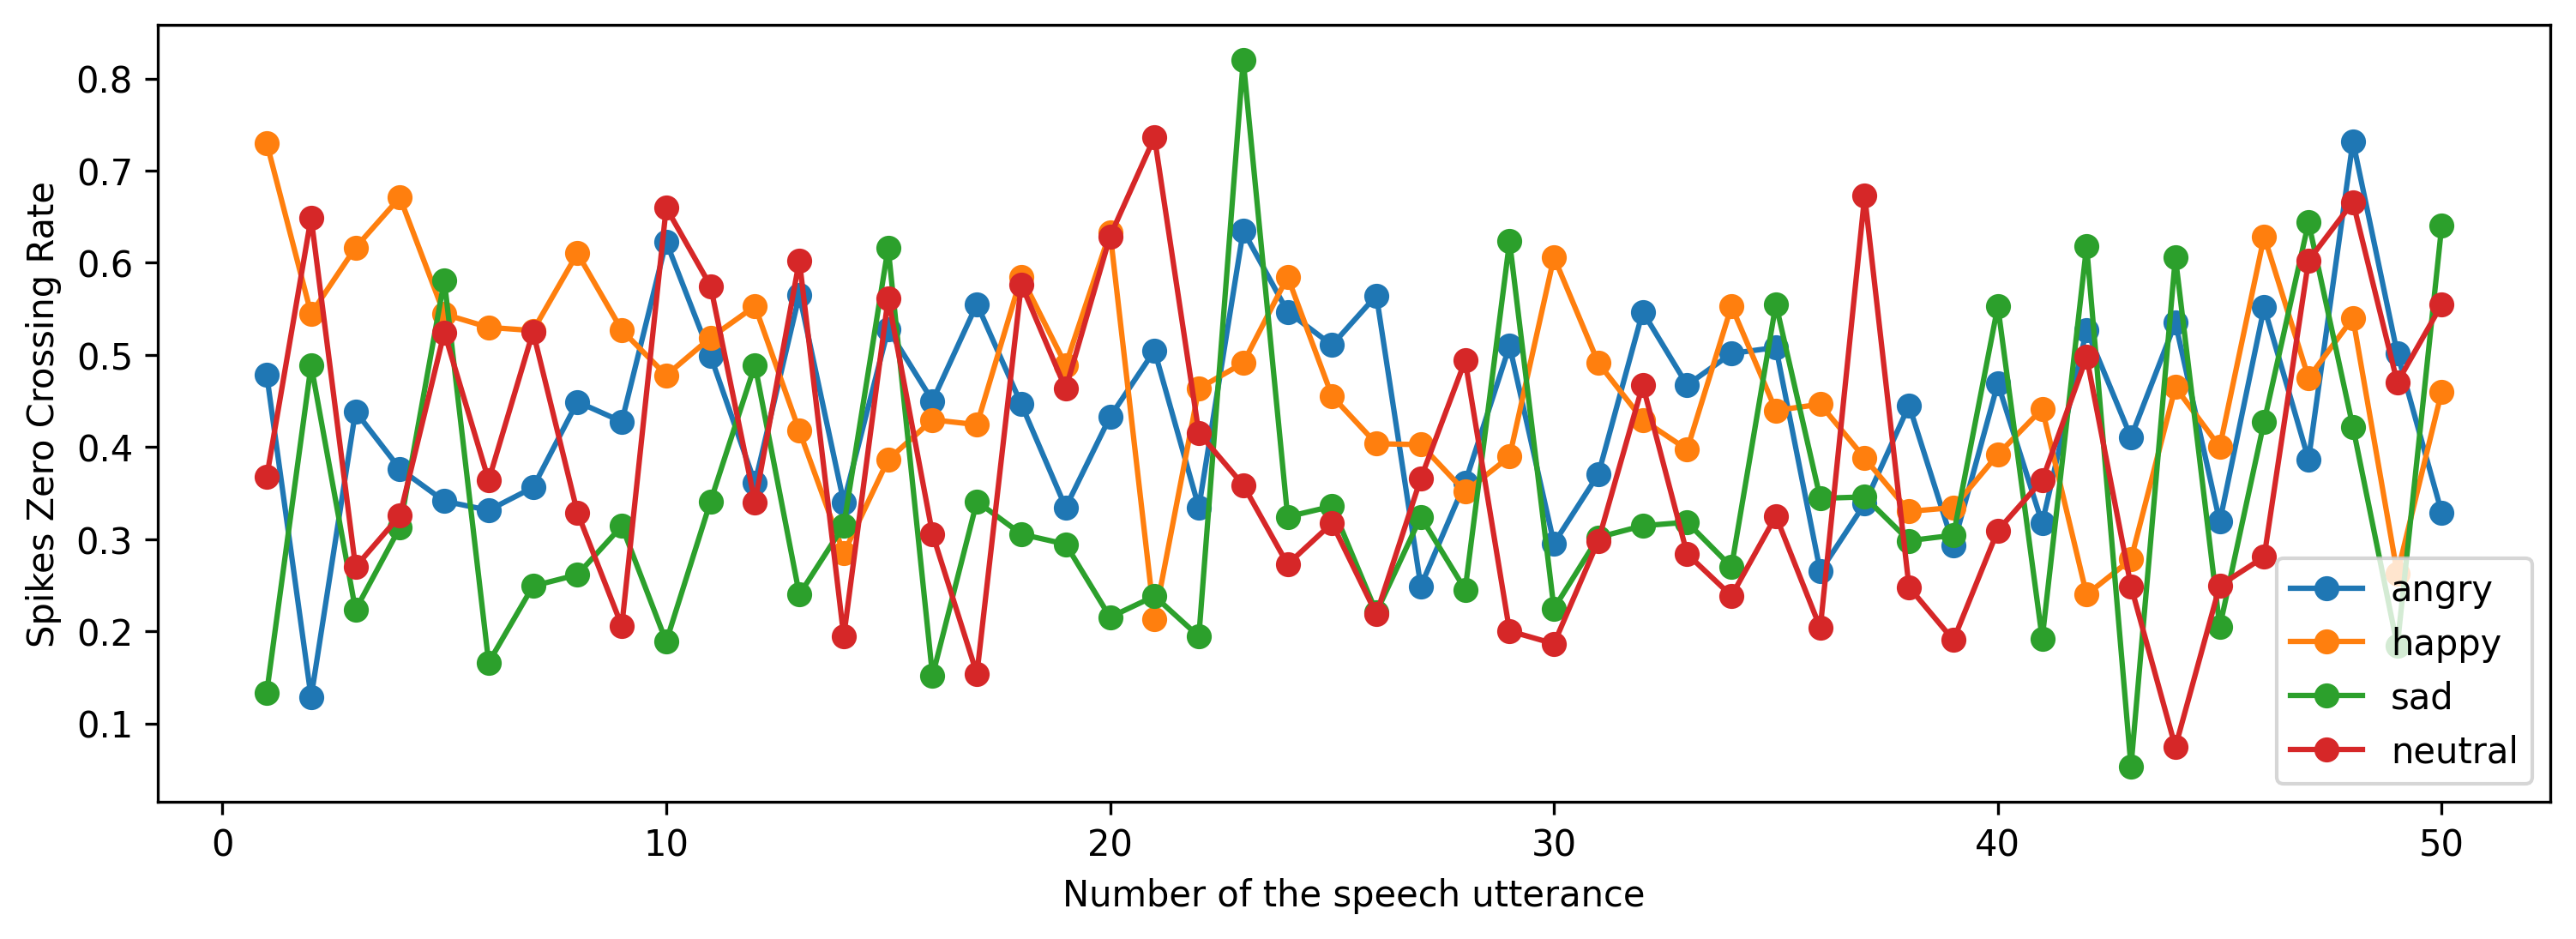
\includegraphics[width=.8\linewidth]{figs/appendix/feature_selection/spikesZCRVar.png}
	\caption{Zero crossing rate spikes values variation plot along 50 audios of speech utterances for all emotions}
	\label{fig:spikesZCRVar}
\end{figure}

\begin{figure}[H]
	\centering
	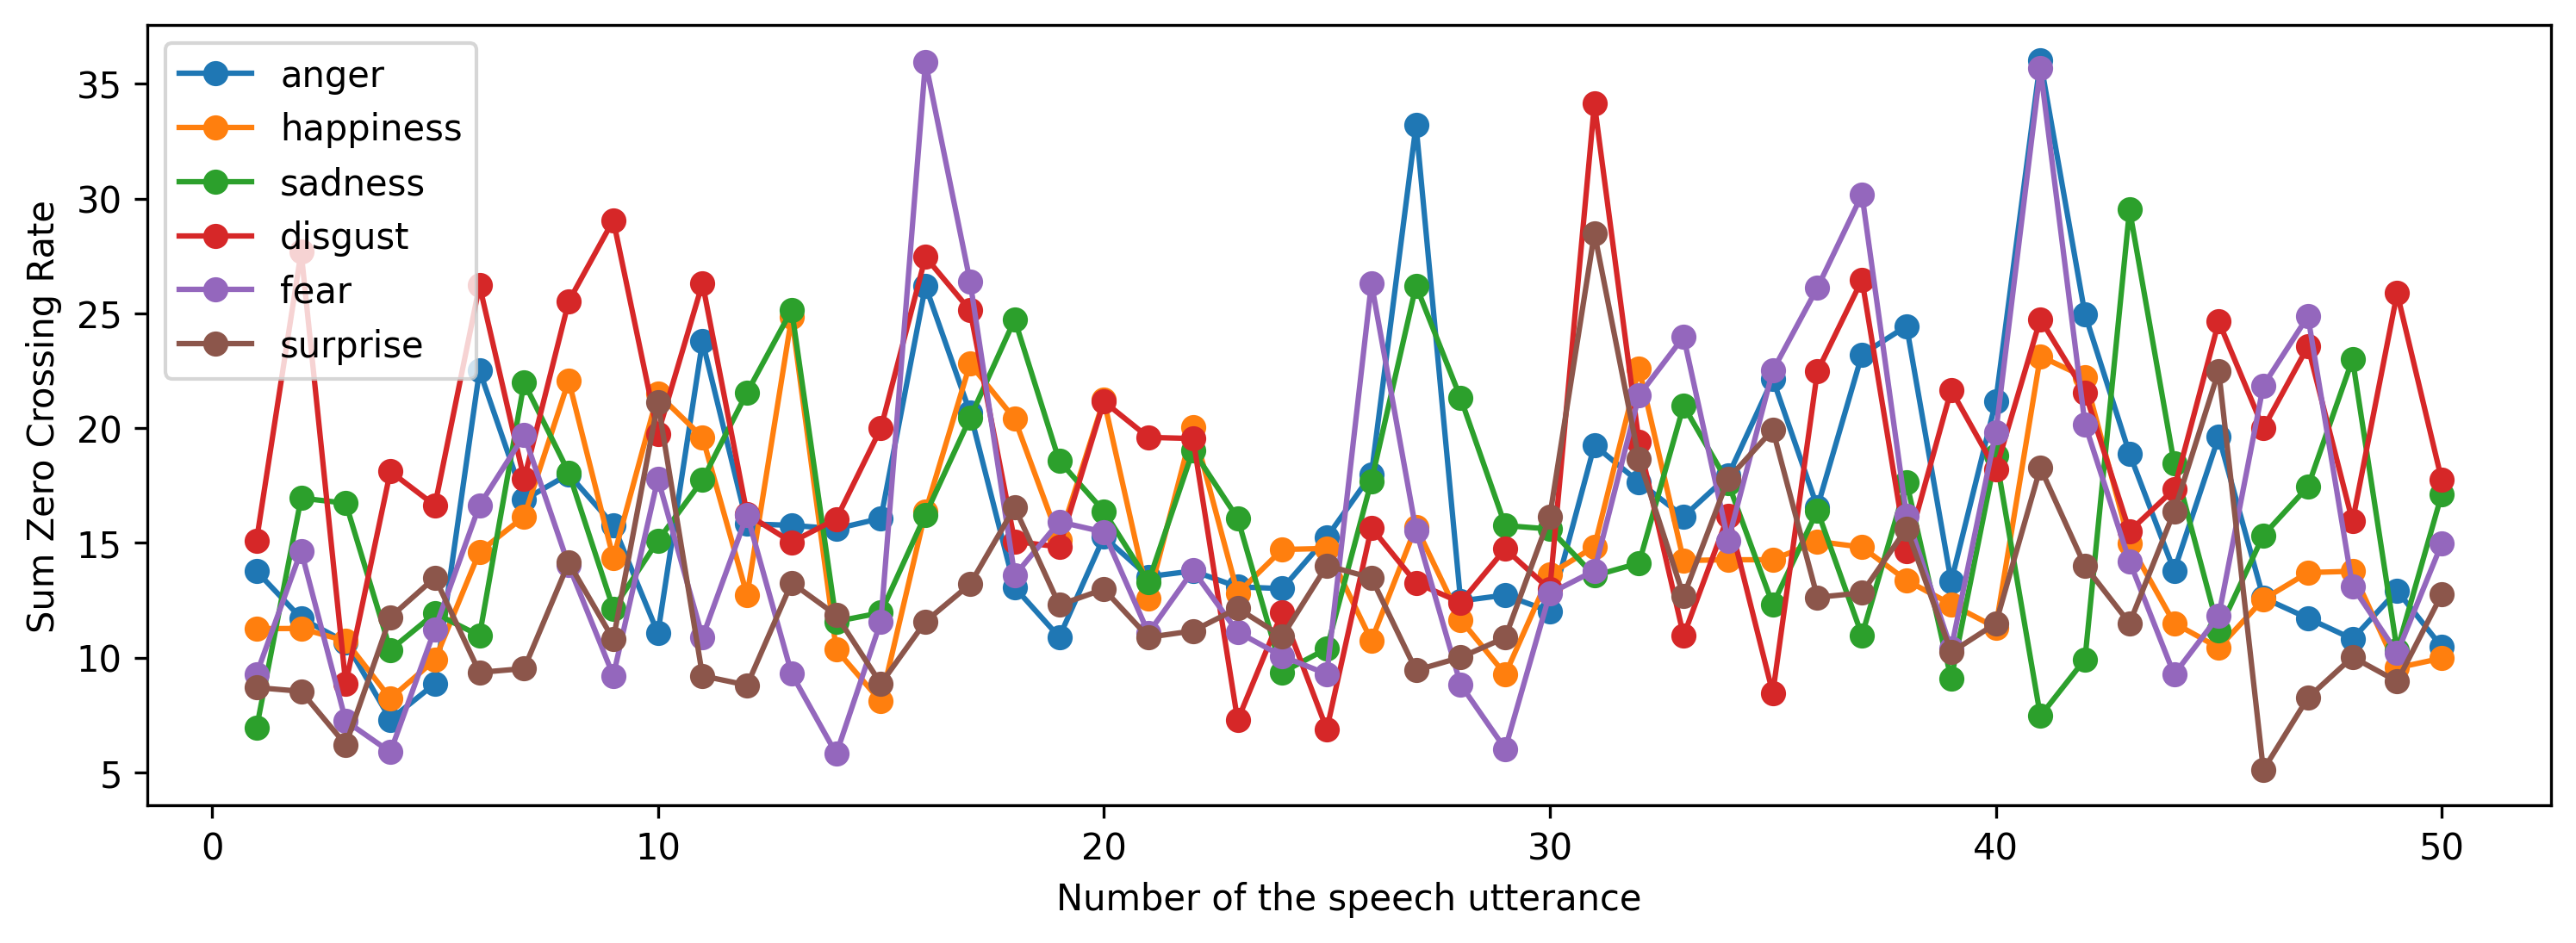
\includegraphics[width=.8\linewidth]{figs/appendix/feature_selection/sumZCRVar.png}
	\caption{Zero crossing rate sum values variation plot along 50 audios of speech utterances for all emotions}
	\label{fig:sumZCRVar}
\end{figure}



\section{Confusion Matrices}  \label{confusionMatrices}

\begin{figure}[H]
	\centering
	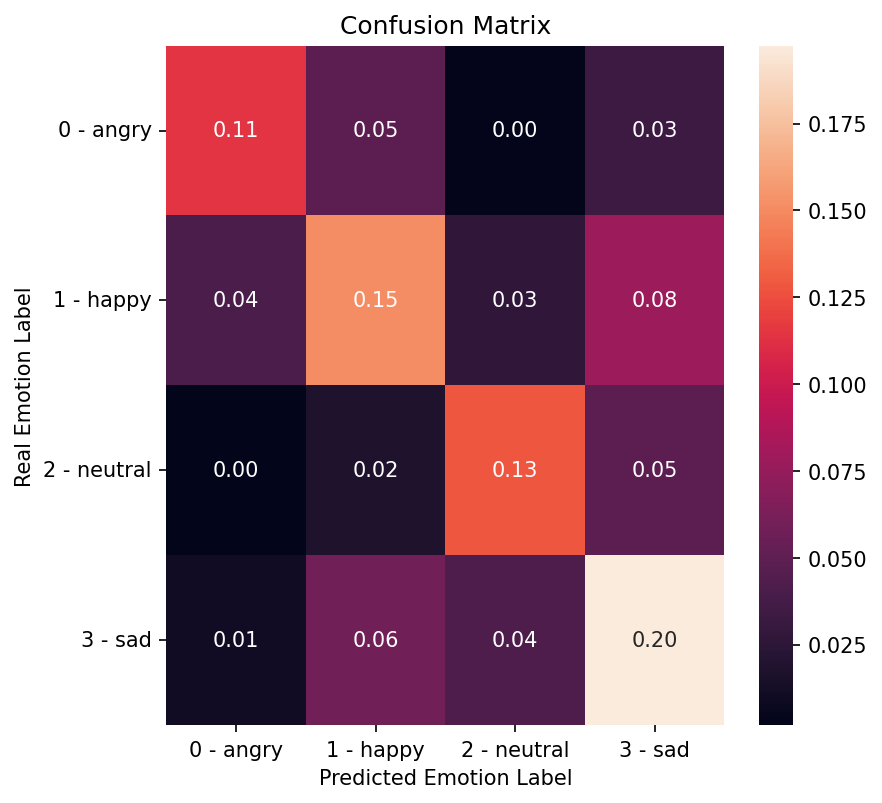
\includegraphics[width=.55\linewidth]{figs/appendix/feature_selection/cmAll.png}
	\caption{Confusion Matrix of a Ridge Classifier Trained using all 327 Extracted Features}
	\label{fig:confMatrix1}
\end{figure}

\begin{figure}[H]
	\centering
	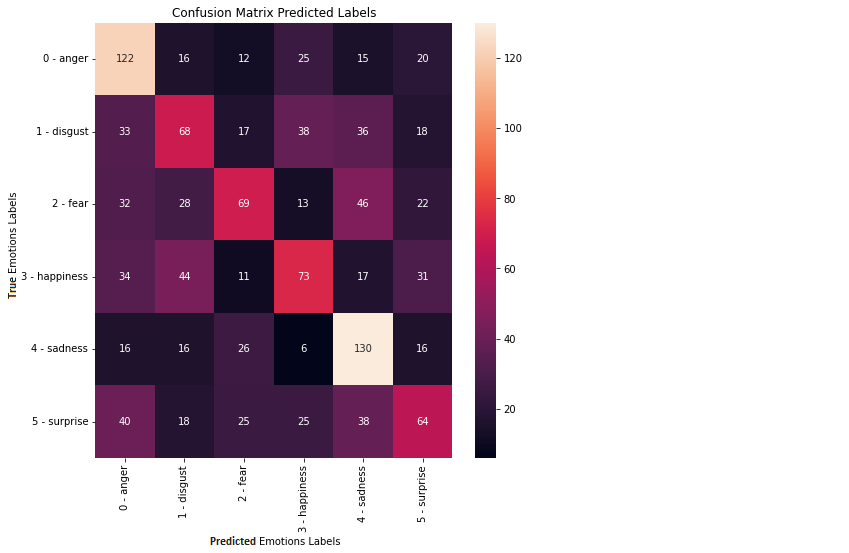
\includegraphics[width=.55\linewidth]{figs/appendix/feature_selection/cmSec.png}
	\caption{Confusion Matrix of a Ridge Classifier Trained using 97 Features After High Correlation Feature Elimination}
	\label{fig:confMatrix2}
\end{figure}


\begin{figure}[H]
	\centering
	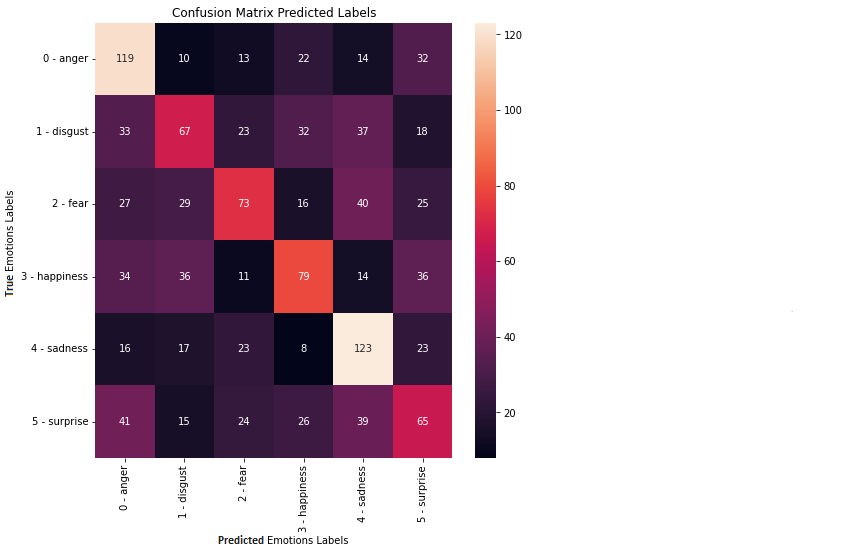
\includegraphics[width=.55\linewidth]{figs/appendix/feature_selection/cmThird.png}
	\caption{Confusion Matrix of a Ridge Classifier Trained using 35 Features After High Correlation and Backward Selection}
	\label{fig:confMatrix3}
\end{figure}


\begin{figure}[H]
	\centering
	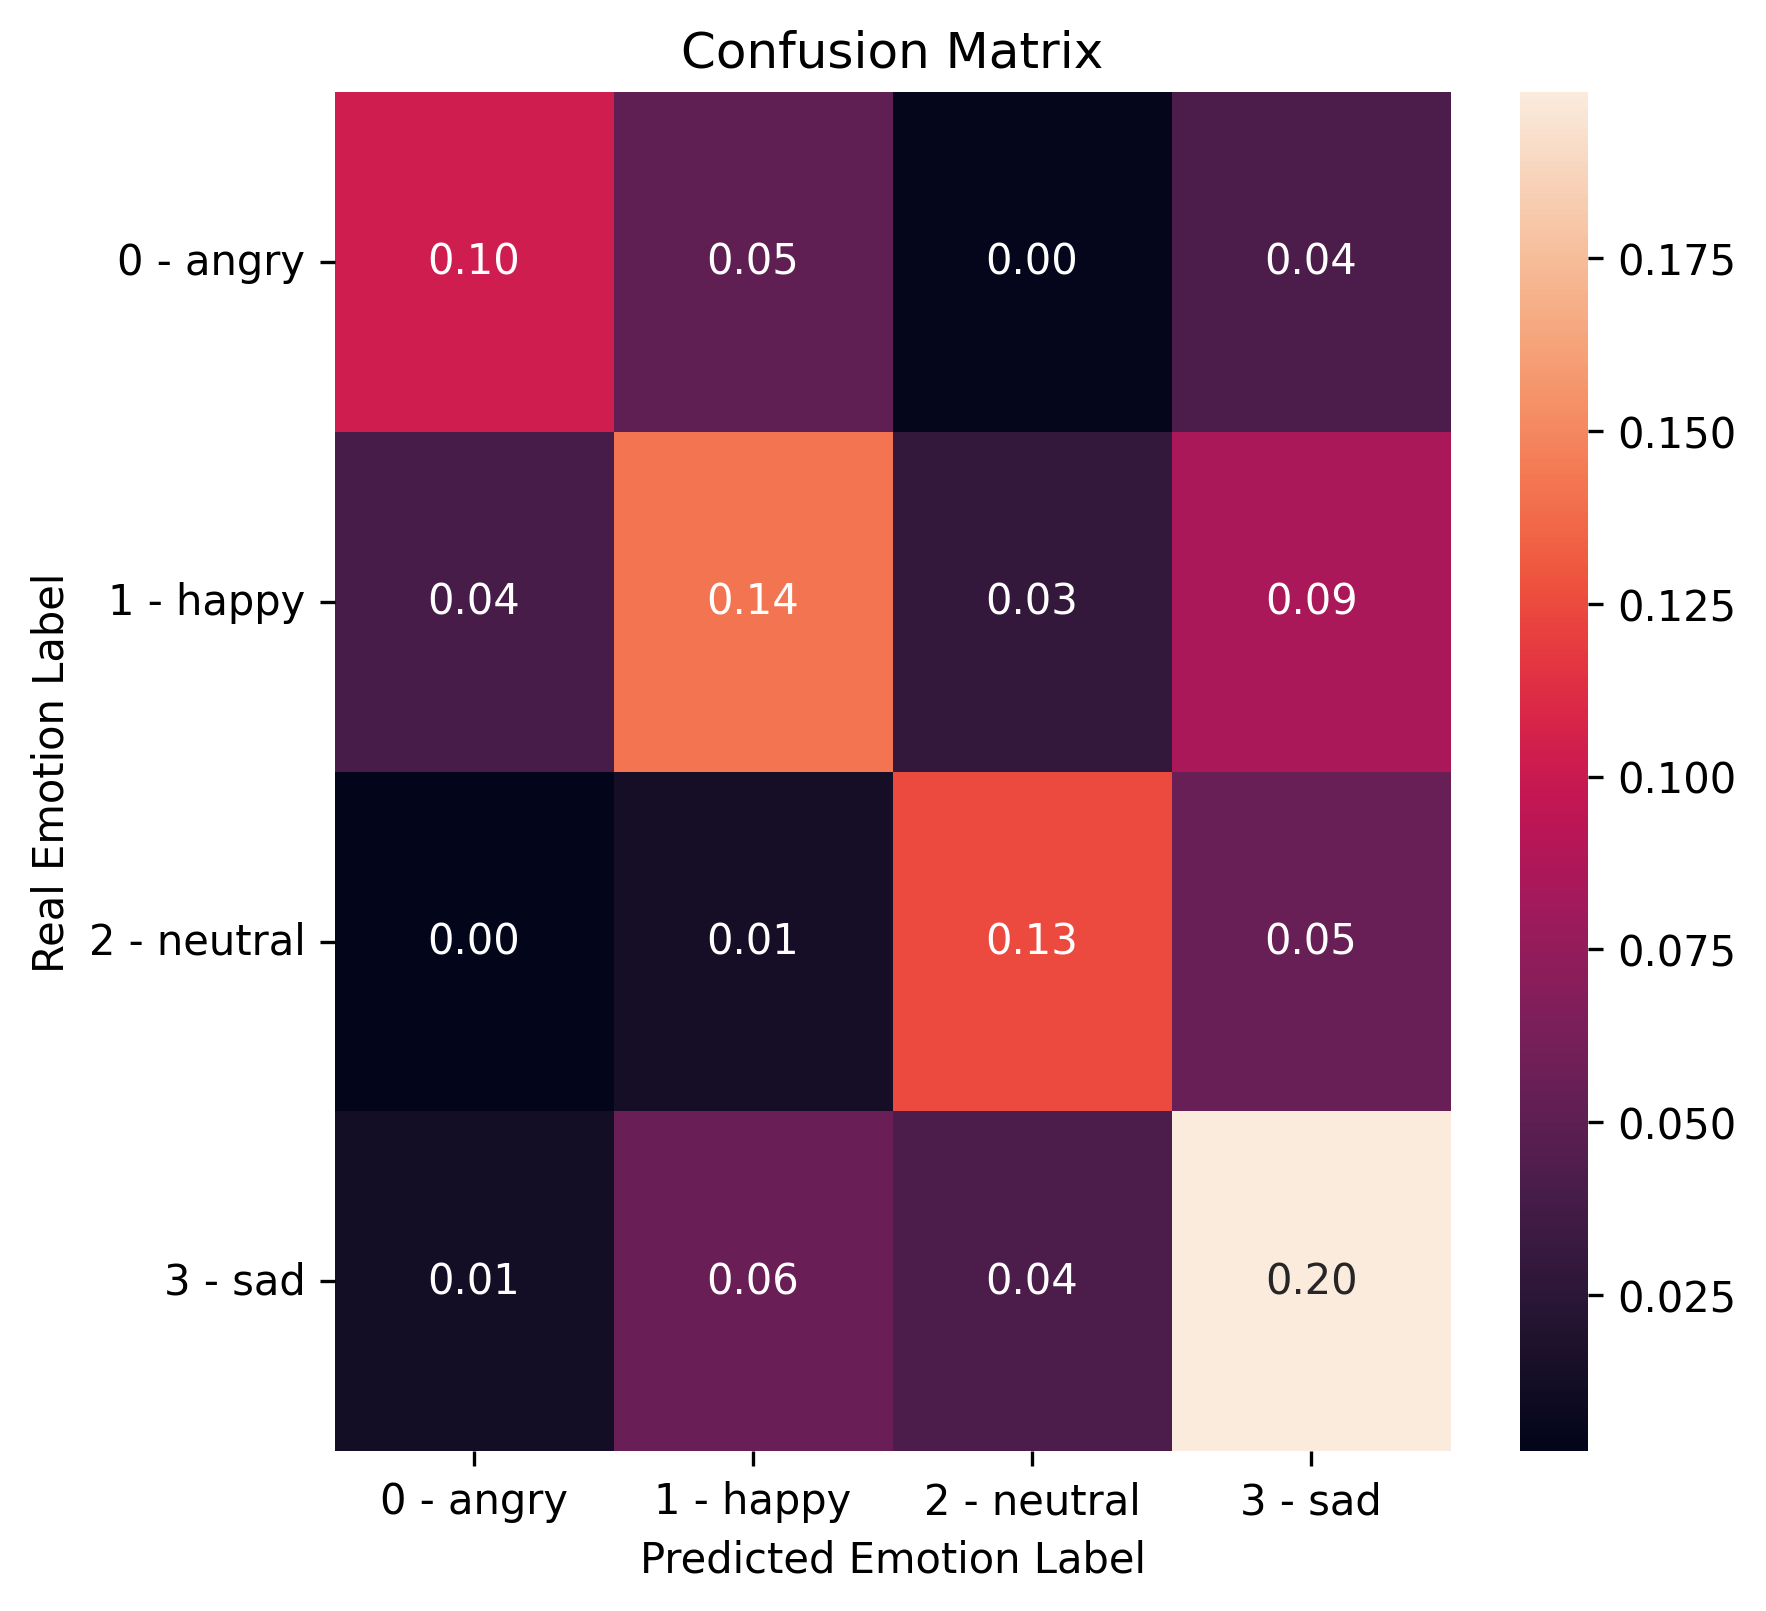
\includegraphics[width=.55\linewidth]{figs/appendix/feature_selection/AdaBoostCM.png}
	\caption{Confusion Matrix of an AdaBoost Classifier.}
\end{figure}

\begin{figure}[H]
	\centering
	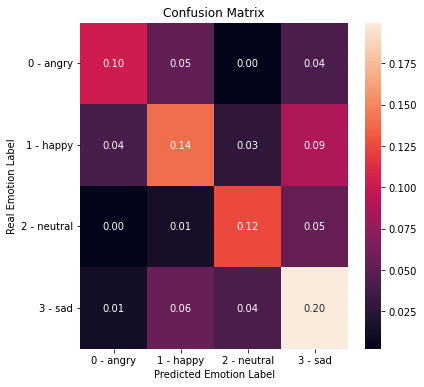
\includegraphics[width=.55\linewidth]{figs/appendix/feature_selection/RandomForestCM.png}
	\caption{Confusion Matrix of a Random Forest Classifier.}
\end{figure}

\begin{figure}[H]
	\centering
	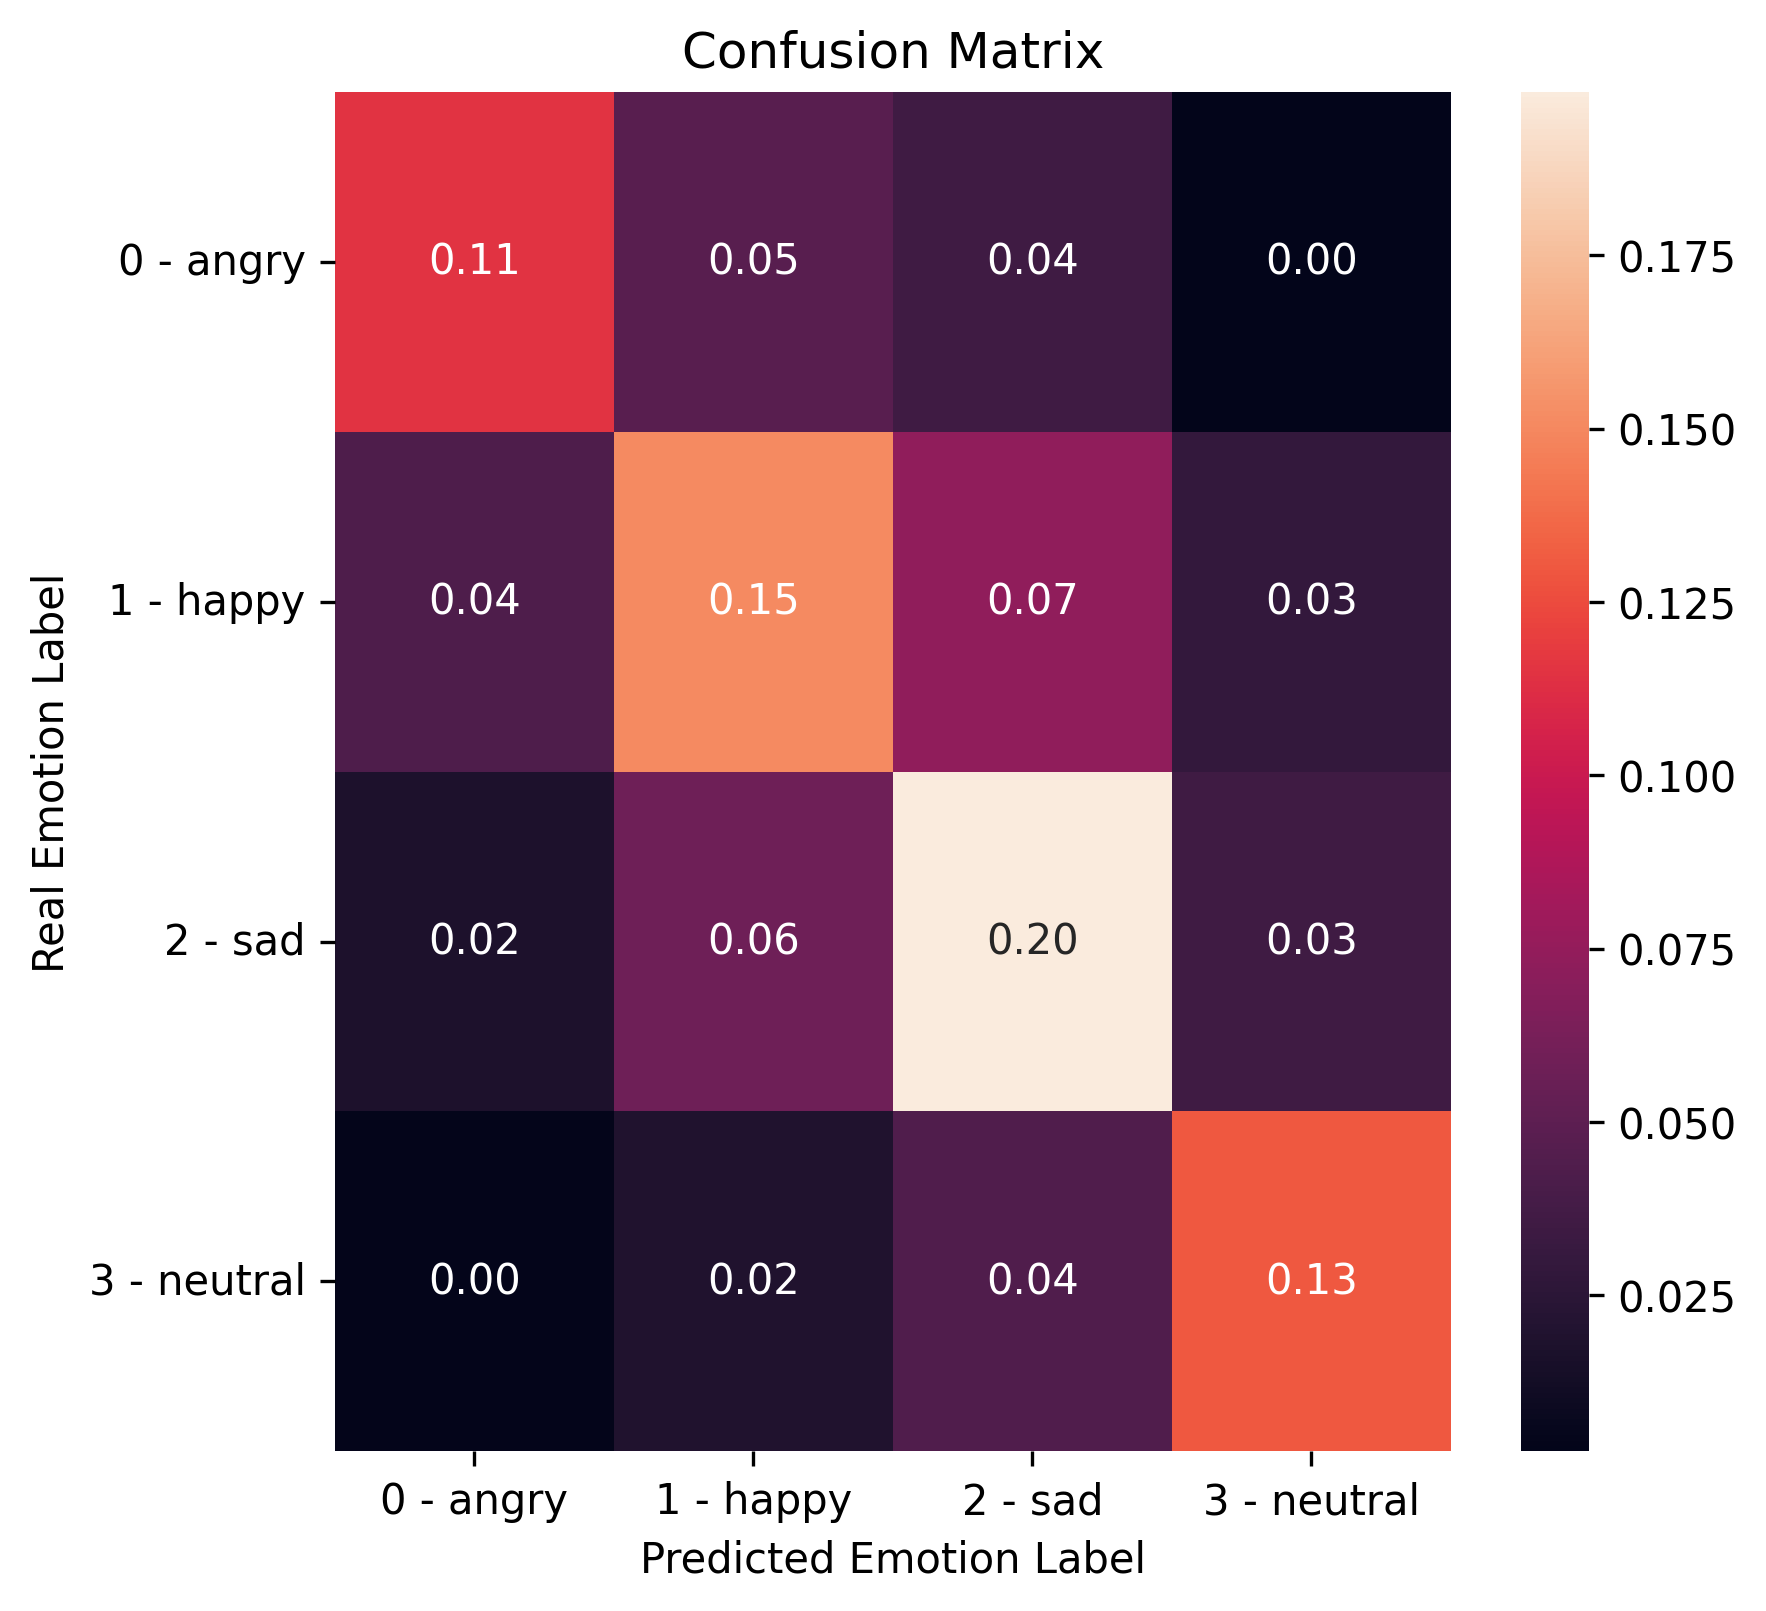
\includegraphics[width=.55\linewidth]{figs/appendix/feature_selection/HistCM.png}
	\caption{Confusion Matrix of a Histogram Gradient Boosting Classifier.}
\end{figure}

\begin{figure}[H]
	\centering
	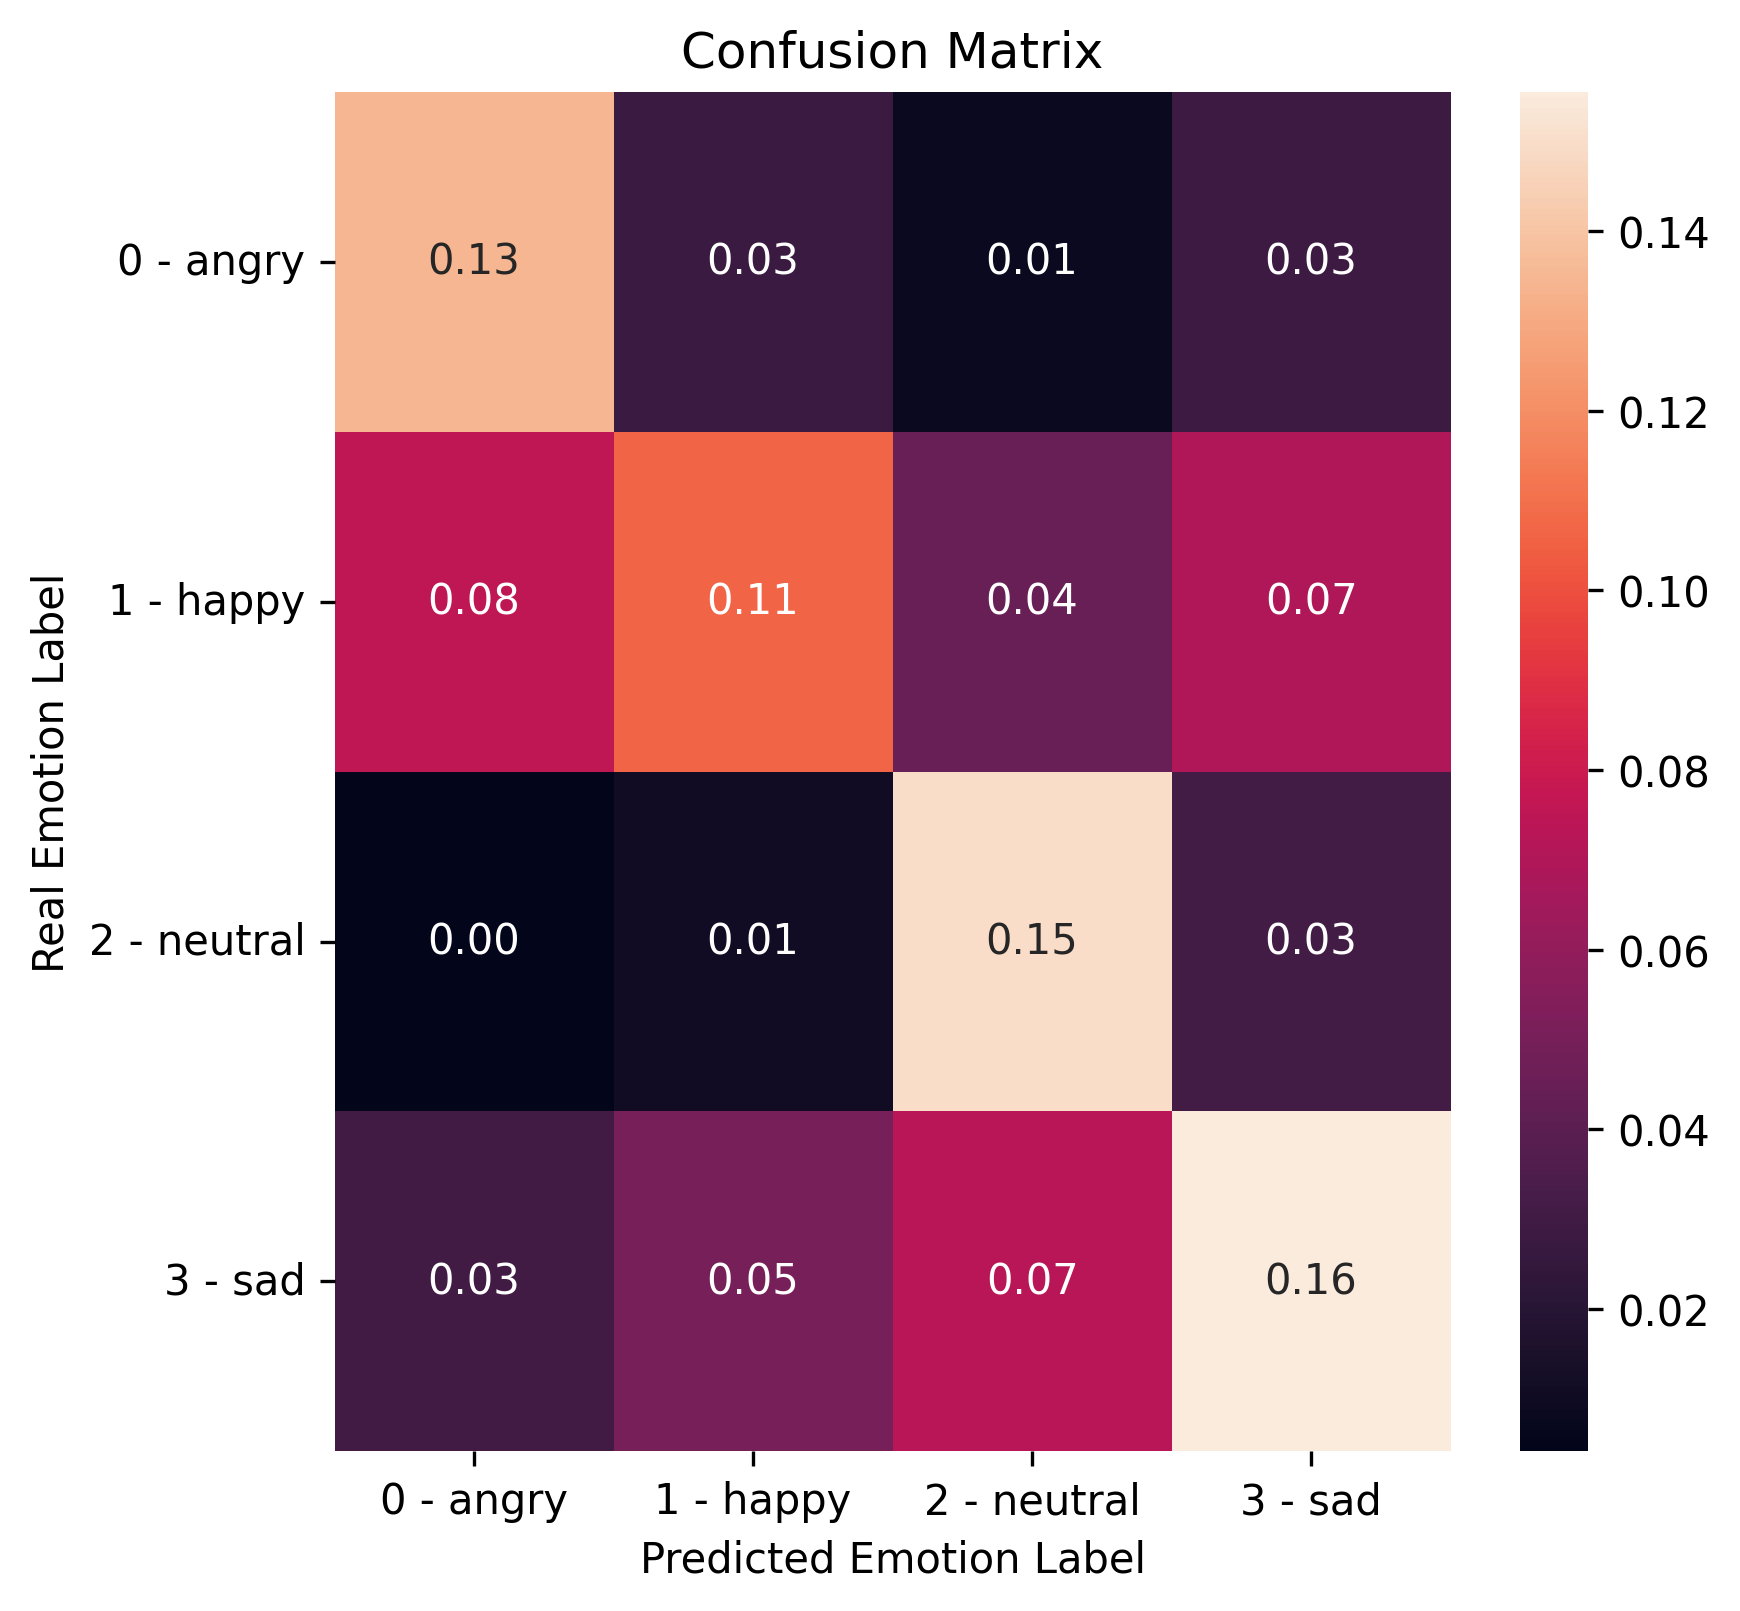
\includegraphics[width=.55\linewidth]{figs/appendix/feature_selection/BalancedForestCM.png}
	\caption{Confusion Matrix of a Balanced Random Forest Classifier.}
\end{figure}

\begin{figure}[H]
	\centering
	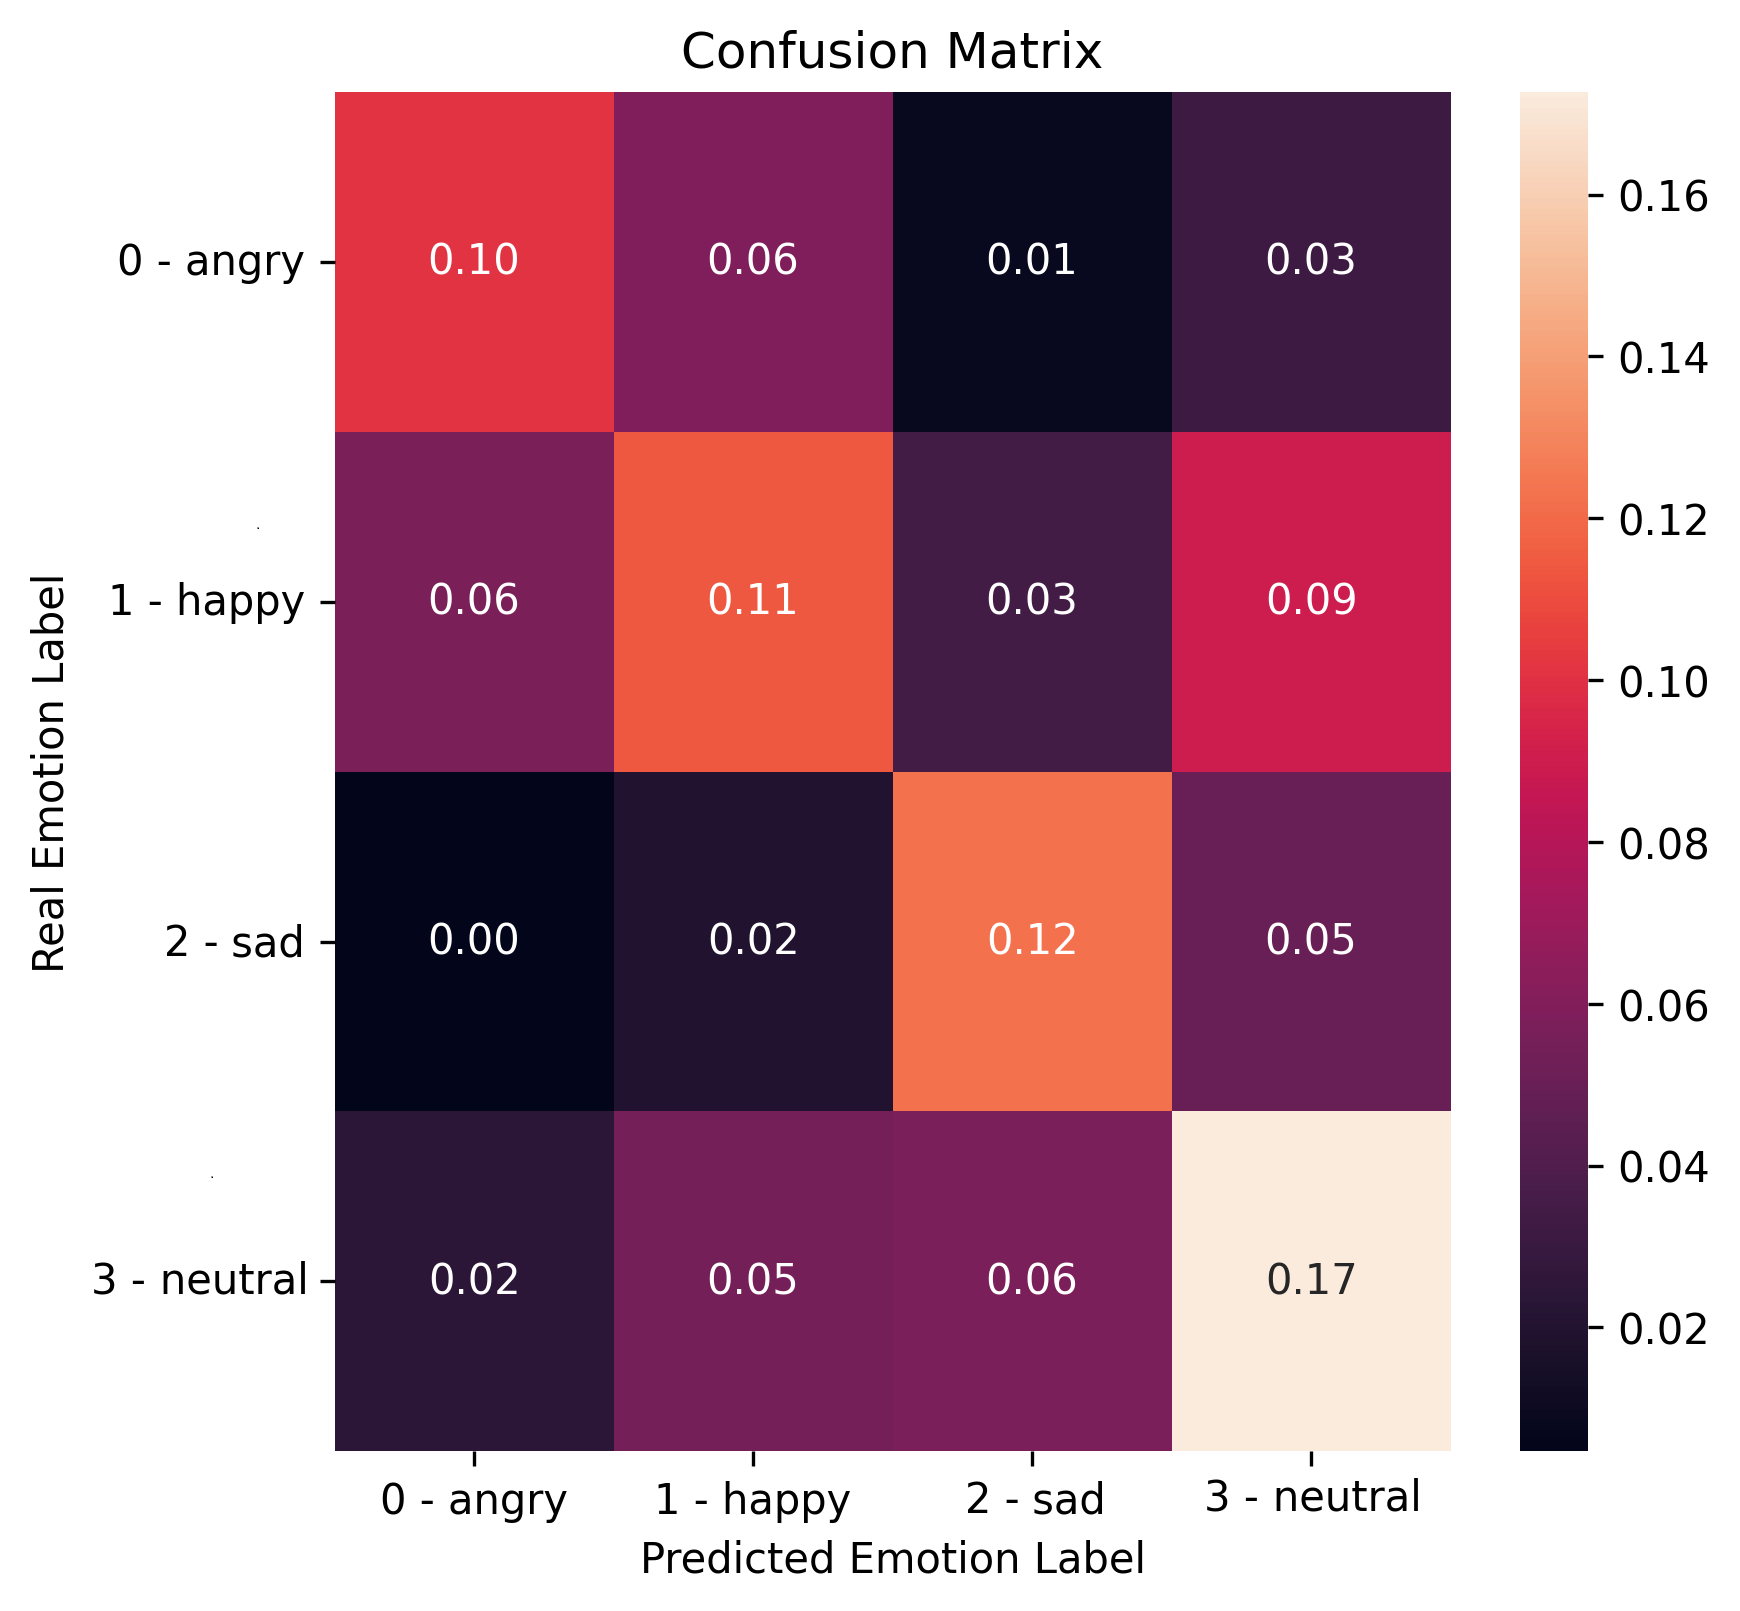
\includegraphics[width=.55\linewidth]{figs/appendix/feature_selection/LSTMCM.png}
	\caption{Confusion Matrix of a \ac{lstm} Classifier.}
\end{figure}

\begin{figure}[H]
	\centering
	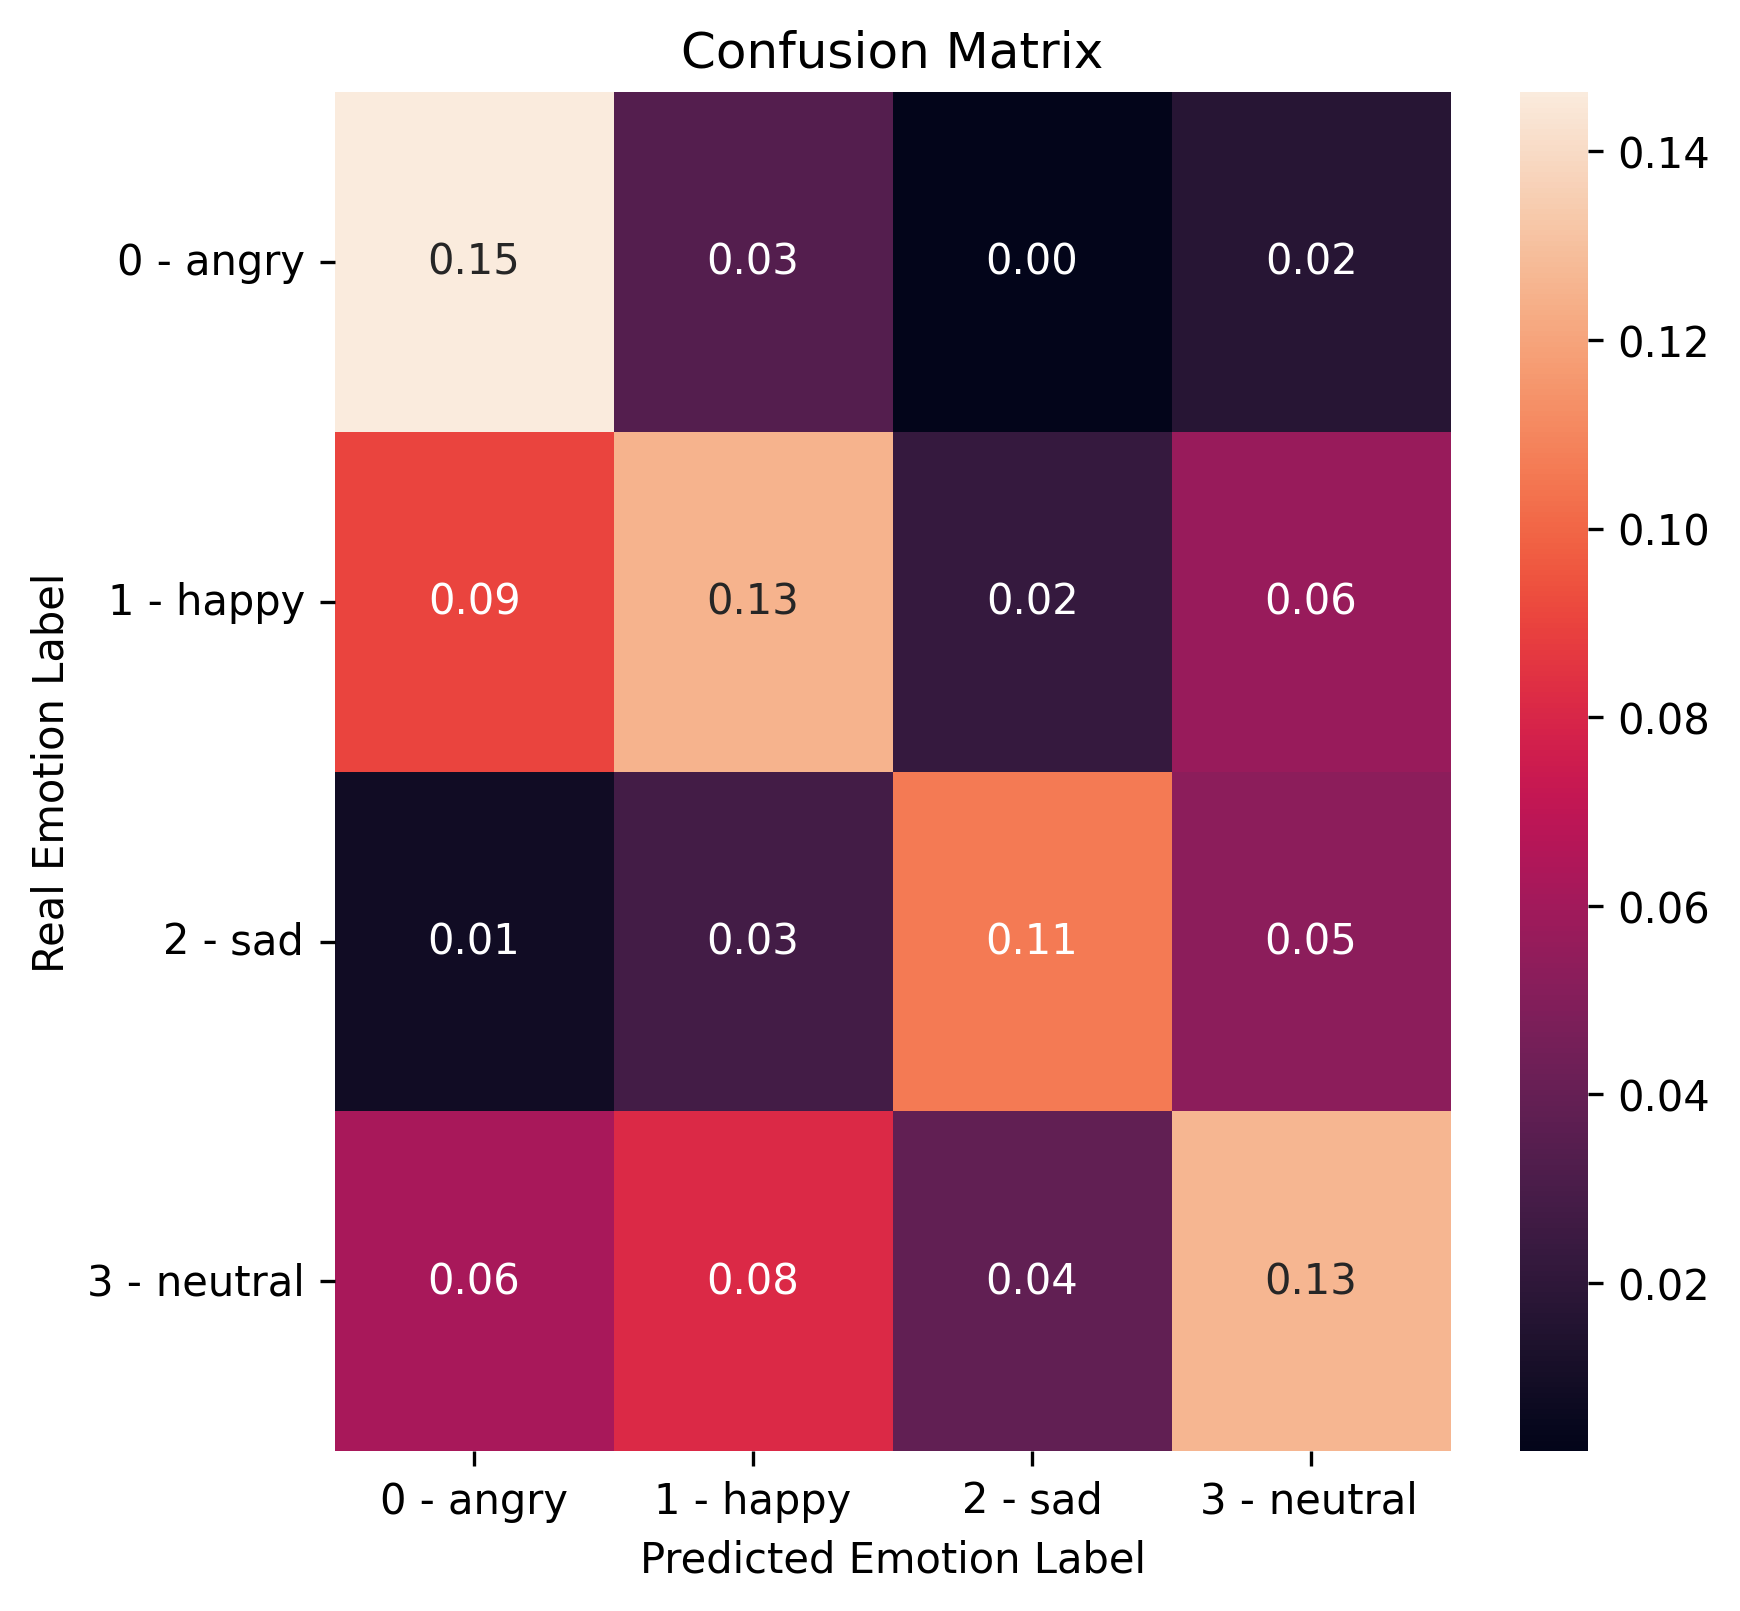
\includegraphics[width=.55\linewidth]{figs/appendix/feature_selection/CNNCM.png}
	\caption{Confusion Matrix of a \ac{cnn} Classifier.}
\end{figure}

\begin{figure}[H]
	\centering
	\includegraphics[width=.55\linewidth]{figs/appendix/feature_selection/LDACM.png}
	\caption{Confusion Matrix of a Linear Discriminant Analysis Classifier.}
\end{figure}

\begin{figure}[H]
	\centering
	\includegraphics[width=.55\linewidth]{figs/appendix/feature_selection/RidgeCM.png}
	\caption{Confusion Matrix of a Ridge Classifier.}
\end{figure}



\section{Something else}

\begin{figure}[H]
	\centering
	\includegraphics[width=1\linewidth]{figs/appendix/IEMOCAP_data_study/activationScatterAllEmotions.png}
	\caption{Scatter Plot of the Annotated Emotions in the Activation Dimension}
	\label{fig:activationScatter}
\end{figure}

\begin{figure}[H]
	\centering
	\includegraphics[width=1\linewidth]{figs/appendix/IEMOCAP_data_study/dominanceScatterAllEmotions.png}
	\caption{Scatter Plot of the Annotated Emotions in the Dominance Dimension}
	\label{fig:dominanceScatter}
\end{figure}


\begin{figure}[H]
	\centering
	\includegraphics[width=1\linewidth]{figs/appendix/IEMOCAP_data_study/neutralScatterViolins.png}
	\caption{Scatter and violin plots of the emotional content of the IEMOCAP corpus in terms of valence, activation, and dominance relative to the neutral emotion}
	\label{fig:neutralScatterViolins}
\end{figure}


\begin{figure}[H]
	\centering
	\includegraphics[width=1\linewidth]{figs/appendix/IEMOCAP_data_study/sadScatterViolins.png}
	\caption{Scatter and violin plots of the emotional content of the IEMOCAP corpus in terms of valence, activation, and dominance relative to the sad emotion}
	\label{fig:sadScatterViolins}
\end{figure}


\begin{figure}[H]
	\centering
	\includegraphics[width=1\linewidth]{figs/appendix/IEMOCAP_data_study/happyScatterViolins.png}
	\caption{Scatter and violin plots of the emotional content of the IEMOCAP corpus in terms of valence, activation, and dominance relative to the happiness emotion}
	\label{fig:happyScatterViolins}
\end{figure}




%%%%%%%%%%%%%%%%%%%%%%%%%%%%%%%%%%%%%%%%%%%%%%%%%%%%%%%
% End of Thesis text 
%%%%%%%%%%%%%%%%%%%%%%%%%%%%%%%%%%%%%%%%%%%%%%%%%%%%%%%

\backmatter

%%%%%%%%%%%%%%%%%%%%%%%%%%%%%%%%%%%%%%%%%%%%%%%%%%%%%%%
% Print all used references
%%%%%%%%%%%%%%%%%%%%%%%%%%%%%%%%%%%%%%%%%%%%%%%%%%%%%%%

\begingroup
\renewcommand{\bibfont}{\footnotesize}
% Redefine References name to Portuguese
% Change if you are using english
\defbibheading{bibliography}[Bibliography]{
	\chapter{#1}
}
\SingleSpacing
\setlength\bibitemsep{8pt}
\printbibliography[heading=bibliography]
\endgroup


%%%%%%%%%%%%%%%%%%%%%%%%%%%%%%%%%%%%%%%%%%%%%%%%%%%%%%%
% Load appendix
%%%%%%%%%%%%%%%%%%%%%%%%%%%%%%%%%%%%%%%%%%%%%%%%%%%%%%%

%\include{appendix-a}
%\include{appendix-b}
%\include{appendix-c}

\end{document}